%%%%%%%%%%%%%%%%%%%%%%%%%%%%%%%%%%%%%%%%%%%%%%%%%%

% Latex Kapitel erstellen. 
% 		Kopiere 'texPandoc/*.tex' nach 'content/tex' 
% 		'content/tex' **Handarbeit... für opt. Ergebnisse!** 
% 		Kopiere 'archiv/inhalt.tex' nach 'content/' 
% 		make -- Latex-PDF erstellen 
% ju 26-Dez-2022 inhalt.tex

%%%%%%%%%%%%%%%%%%%%%%%%%%%%%%%%%%%%%%%%%%%%%%%%%%

% content/

\chapter{01-Grundlagen-Verbrennungsmotor}
%%ju 26-Dez-22 01-Grundlagen-Verbrennungsmotor.tex
\section{Motorbauformen}\label{motorbauformen}

\begin{itemize}
\item
  Reihenmotor, V-Motor, VR-Motor, Boxermotor
\item
  Hubkolbenmotor, Kreiskolbenmotor
\end{itemize}

\section{Hubraum - Brennraum -
Verdichtungsraum}\label{hubraum-brennraum-verdichtungsraum}

$\text{Hubraum} \, V_h = \frac{\pi \cdot d^2}{4} \cdot s \,[cm^3]$

$\text{Gesamthubraum} \, V_H = V_h \cdot z$

$\text{Brennraum} = V_h + V_c$

$\text{Verdichtungsraum} \, V_c = \frac{V_h}{\epsilon - 1}$

$\text{Verdichtungsverhältnis} \, \epsilon = \frac{V_h + V_c}{V_c}$

\section{Arbeitsweise}\label{arbeitsweise}

\begin{enumerate}
\def\labelenumi{(\arabic{enumi})}
\item
  Vier-Takt-Arbeitsverfahren (1 Arbeitsspiel = 2 Kurbelwellenumdrehungen
  = 4 Kolbenhübe)
\item
  Zwei-Takt-Arbeitsverfahren (1 Arbeitsspiel = 1 Kurbelwellenumdrehung =
  2 Kolbenhübe)
\end{enumerate}

\section{Ansaugen}\label{ansaugen}

\begin{itemize}
\item
  Abwärtsgehen des Kolbens
\item
  Volumenvergrößerung, Druckdifferenz (Zylinderdruck versus höhere
  Außendruck)
\item
  Einströmen der Luft (Ansaugen der Luft)
\item
  zündfähiges Kraftstoff-Luft-Gemisch innen/außen bilden (Zylinder,
  Ansaugrohr)
\item
  Kraftstoff (Kohlenstoff -- Wasserstoff - Verbindung)
\end{itemize}

\subsection{Luftdruck}\label{luftdruck}

Luftdruck in Abhängigkeit der geodätischen Höhe

Luftdruck bezogen auf Meereshöhe $(1013~hPa = 1013~mbar, ca.\,1~bar)$

Erdanziehung ist von der Masse abhängig

Das Gewicht der Umgebungsluft drückt auf die Erdoberfläche und erzeugt
einen Druck, Atmosphärendruck.

\subsection{Absolutdruck}\label{absolutdruck}

Druck gegenüber Null (Vakuum, luftleeren Raum)

\subsection{Relativer Druck}\label{relativer-druck}

Druck messen gegenüber Absolutdruck

\subsection{Zusammensetzung der Luft
(Prüfung)}\label{zusammensetzung-der-luft-pruefung}

\begin{itemize}
\item
  $78~\%$ Stickstoff
\item
  $21~\%$ Sauerstoff
\item
  $0,9~\%$ Edelgase
\item
  $0,1~\%$ Partikel, Feinstaub (Zell Gängigkeit, Blutkreislauf,
  Erbgutveränderung > Mutation)
\item
  $0,040~\% ~ CO_2$
\end{itemize}

\section{Verdichten}\label{verdichten}

\begin{itemize}
\item
  Aufwärtsgehen des Kolbens
\item
  Kraftstoff-Luft-Gemisch wird verdichtet
\end{itemize}

\subsection{Hoch verdichtete Motoren}\label{hoch-verdichtete-motoren}

$10:1$

\subsection{Verdichtungsverhältnis}\label{verdichtungsverhaeltnis}

\begin{itemize}
\item
  \textbf{Mazda Motor:} $14:1$
\item
  \textbf{Turbo Motor:} $7 - 8:1$
\item
  \textbf{Direkt:} $17 - 18:1$
\item
  \textbf{Indirekt} (Wirbel, Vorkammer): $21 - 36:1$

  \begin{itemize}
  \item
    Vorkammer > Kugel > Wärmeabgabe
    > höher Verdichten
  \end{itemize}
\end{itemize}

\subsection{Wärme}\label{waerme}

entsteht durch Reibung, Form von Energie, Bewegungsenergie kleiner
Teilchen

\subsection{Wärmeabführung}\label{waermeabfuehrung}

an der Oberfläche, Luft (Isolator)

\subsection{Verdichten z.~B. 10:1}\label{verdichten-z.-b.-101}

$10~l$ großes Volumen wird auf den zehnten Teil verkleinert, also
$1~l$

maximales Volumen zu minimales Volumen

Vgl. >>\emph{Kapitel Rechenbeispiele / Motor - Hubraum - Verdichtung}<<

\subsection{Verdichtungsendtemperatur}\label{verdichtungsendtemperatur}

$600 - 900^\circ\text{C}$ (Diesel: Zündung wird eingeleitet)

\subsection{Entzündungstemperatur
Diesel}\label{entzuendungstemperatur-diesel}

$230 - 250^\circ\text{C}$

\subsection{Zündverzug}\label{zuendverzug}

$Entflammungsphase: \frac{1}{1000} s$

Ziel: Vollständige Verbrennung (feine Zerstäubung und hohe Temperaturen,
das muss schnell gehen)

\begin{enumerate}
\def\labelenumi{(\arabic{enumi})}
\item
  \textbf{Benzin} Beginn Zündfunken bis zur Verbrennung
\item
  \textbf{Diesel} Beginn des Einspritzens bis zur Verbrennung
\end{enumerate}

\subsection{Thermodynamischer Kreisprozess (keine
Prüfung)}\label{thermodynamischer-kreisprozess-keine-pruefung}

Wärmekraftmaschine: Verhältnis von Druck, Volumen und Temperatur beim
Verdichten

Verhindert man die Ausdehnung, z.~B. beim Verdichten, so verdoppelt sich
der Druck.

Pro Grad der Erwärmung steigt der Druck um 273sten Teil seines Volumens
im geschlossenen System

Erwärmt man das Gas um $273~K$, so dehnt es sich auf das doppelte
Volumen aus. Die Temperatur steigt und damit der Druck.

Grundlage: \textbf{1. Satz der Thermodynamik} >>Die Energie bleibt in
einem geschlossenen System konstant.<<

\textbf{Faktor 2} $\Rightarrow \frac{546}{273}$

Ziel: von $20^\circ\text{C} \Rightarrow 600^\circ\text{C}$
Verdichtungsendtemperatur

z.~B. Verdichtung: $(10:1)$ $1~bar \Rightarrow 20~bar$
Verdichtungsenddruck $(10~bar \cdot 2 = 20~bar)$

Vgl. >>\emph{Kapitel Rechenbeispiele / Druck - Volumen - Temperatur}<<

\textbf{Diesel} Gleichdruckverbrennung \textbf{Benzin}
Gleichraumverbrennung \textbf{Anwendung} Zylinderabschaltung, Studium

\subsection{Grad Celsius}\label{grad-celsius}

als Fixpunkte werden die Temperaturen vom Gefrier- $(0^\circ\text{C})$
und Siedepunkt $(100^\circ\text{C})$ des Wassers verwendet

\subsection{Aggregatzustand}\label{aggregatzustand}

physikalischer Zustand eines Stoffs. Beispiel: fest, flüssig, gasförmig,
plasma

\subsection{Kelvin}\label{kelvin}

absoluten Nullpunkt der Teilchen $(0K = -273^\circ\text{C})$

$0~K = -273,15^\circ\text{C}$

$273,15~K = 0^\circ\text{C}$

$373,15~K = 100^\circ\text{C}$

\textbf{Umrechnung}

$Kelvin = T_{Grad~Celsius} + 273,15$

$Grad~Celsius = T_{Kelvin} - 273,15$

\section{Arbeiten}\label{arbeiten}

\begin{itemize}
\item
  Verbrennung wird durch den Zündfunken eingeleitet
\item
  Die Expansion der Gase treibt den Kolben nach UT
\item
  Wärmeenergie wird in mechanische Energie umgewandelt
\end{itemize}

\subsection{Verbrennungstemperatur}\label{verbrennungstemperatur}

$2000 - 2500^\circ\text{C}$

\subsection{Kolbenmaterial}\label{kolbenmaterial}

Aluminium-Silizium-Legierung

\subsection{Thermische Belastung
Kolben}\label{thermische-belastung-kolben}

\textbf{Problem} Kolbenbodentemperaturen

\begin{enumerate}
\def\labelenumi{(\arabic{enumi})}
\item
  $390^\circ\text{C}$ Diesel
\item
  $290^\circ\text{C}$ Benziner
\item
  $421^\circ\text{C}$ Stahlkolben
\end{enumerate}

\textbf{Kerbe} = Sollbruchstelle

\subsection{Kolbenfläche berechnen}\label{kolbenflaeche-berechnen}

$A = \frac{\pi \cdot d^2}{4} = [mm^2]$

Vgl. >>\emph{Kapitel Rechenbeispiele / Druckberechnung am Pleuellager}<<

\subsection{Kolbenwärme abführen}\label{kolbenwaerme-abfuehren}

\begin{itemize}
\item
  Kolbenboden
\item
  $80~\%$ über 1. Kolbenring, Kompressionsring, Minutenring,
  (trapezförmig)
\item
  Zylinderwand
\end{itemize}

\subsection{Kolbenkippen Ursache}\label{kolbenkippen-ursache}

\begin{itemize}
\item
  Druckverlagerung
\item
  Desachsierung des Kolbens
\item
  Wann liegt der Kolbendruck an?
\item
  Wann Übergehen der Kolbengleitbahnen (deshalb die Desachsierung des
  Kolbens)
\item
  Welche Kolbenbauform?
\item
  ausreichend langes Kolbenhemd $\to$ Problem mehr Masse
\item
  Masse einmal beschleunigt, wenn Kolben nach unten (möchte durch die
  Ölwanne in den Boden) oder Kolben nach oben (durch die Motorhaube in
  den Himmel) davon hält das Pleuel ab
\end{itemize}

\section{Ausstoßen}\label{ausstossen}

\begin{itemize}
\item
  Abgase verlassen mit Überschallgeschwindigkeit den Zylinder
\end{itemize}

\subsection{Abgastemperatur}\label{abgastemperatur}

$600 - 900^\circ\text{C}$

\subsection{Wirkungsgrad (Effizienz)}\label{wirkungsgrad-effizienz}

\begin{enumerate}
\item
  Dieselmotoren ca. $46~\%$ und
\item
  Ottomotoren ca. $35~\% \to$ werden in \textbf{Bewegungsenergie} als
  Antriebsenergie für Motor verwendet
\end{enumerate}

Rest in \textbf{Reibung und Wärme}

\subsection{Wie bewegt sich die
Kurbelwelle?}\label{wie-bewegt-sich-die-kurbelwelle}

\textbf{Ungleichförmige Drehbewegung}

Hubkolbenbewegung Reihenmotor (abhängig Zylinderanzahl, Zündreihenfolge)

Kompensieren: Kurbelwellenrad exzentrisch ausgeführt (unterschiedliche
Hebellängen)

Beschleunigt (Zündungstakt)

\begin{itemize}
\item
  alle zwei NW Umdrehungen
\item
  alle vier KW Umdrehungen
\end{itemize}

\subsection{Hydrodynamischer
Schmierkeil}\label{hydrodynamischer-schmierkeil}

\begin{itemize}
\item
  durch ungleichförmige Drehbewegung
\item
  wird eine Volumenvergrößerung zwischen Kurbelwelle und Lagerung
  erreicht
\item
  dadurch ein Einströmen des Lageröls in die Lagerstelle begünstigt
\item
  Und wenn jetzt der Verbrennungsdruck durch die Verbrennung erzeugt auf
  die Kurbelwellenlagerstelle schneller erfolgt, als die Verdrängung des
  Öls aus der Lagerstelle heraus
\item
  Aufschwimmen auf unserem Lager
\item
  Wir bewegen uns auf dem hydrodynamischen Schmierkeil
\item
  Ist in der Lage hohe Drücke auszuhalten
\end{itemize}

Wie kann es sein, dass ich mit einem Versorgungsdruck von $5~bar$
einen Öldruck in den Lagern der Kurbelwelle einen Spitzendruck bis
$1000~bar$ kompensieren kann > Hydrodynamischer
Schmierkeil

Vgl. >>\emph{Kapitel Rechenbeispiele / Druckberechnung am Pleuellager}<<

\section{Kurbelgehäusearten}\label{kurbelgehaeusearten}

\begin{enumerate}
\item
  Closed-Deck-Ausführung

  \begin{itemize}
  \item
    Dichtfläche bis auf Kühl- oder Ölkanäle geschlossen gegenüber
    Zylinderkopf
  \item
    Niederdruckguss-Verfahren (AlSi-Legierung)
  \end{itemize}
\item
  Open-Deck-Ausführung

  \begin{itemize}
  \item
    Wassermantel um die Zylinderbohrungen offen gegenüber Zylinderkopf
    (geringe Steifigkeit, erfordert Metall-Zylinderkopfdichtung)
  \item
    Druckgussverfahren
  \end{itemize}
\end{enumerate}

\section{Zylinderkopfdichtung}\label{zylinderkopfdichtung}

Gasabdichtung bei allen Betriebszuständen

\begin{enumerate}
\item
  Metall-Weichstoff-Zylinderkopfdichtung
\item
  Metall-Zylinderkopfdichtung
\end{enumerate}

\chapter{01-Loesung-Grundlagen-Verbrennungsmotor}
%%ju 13-Aug-22 01-Loesung-Grundlagen-Verbrennungsmotor.tex
\textbf{Bemerkung}, die in Klammern stehende Kommentare gehören nicht
zur Beantwortung der Frage.

\textbf{1) Ein Verbrennungsmotor benötigt zum Arbeiten ein
Kraftstoff-Luft-Gemisch. Was ist Kraftstoff und was ist Luft?}

Fachbuch (\textcite{brand:2020:fachkundeKfz} S. 29)

\begin{enumerate}
\def\labelenumi{(\arabic{enumi})}
\item
  \textbf{Kraftstoffe} sind hauptsächlich Kohlen - Wasserstoff -
  Verbindungen (geringer Anteil Schwefel $\to$ Schmierung). Die Anzahl
  der Atome und deren Verbindungen bestimmen die Art des Kraftstoffes.
  Zur Verbesserung der Eigenschaften werden Ihnen Additive zugefügt.
\item
  \textbf{Luft} ist ein Gasgemisch aus
\end{enumerate}

\begin{itemize}
\item
  $78~\%$ Stickstoff
\item
  $21~\%$ Sauerstoff
\item
  $0,9~\%$ sonstige Gase (Edelgase)
\item
  $0,1~\%$ Schwebeteilchen (Partikel, Feinstaub, Sandstrahl verschleiß
  $\to$ Luftmassenmesser)
\item
  ($0,040~\% ~ CO_2$)
\end{itemize}

\textbf{2) Unterscheiden Sie Boxer-Motor und 180 Grad V-Motor}

\textbf{Boxer-Motor} arbeiten die Kolben der gegenüberliegenden Zylinder
aufeinander zu. Es befinden sich also beide zeitgleich im oberen oder
unteren Totpunkt. Um dies zu ermöglichen, benötigt der Boxer-Motor einen
Kurbelzapfen je Kolben.

(flache Bauweise, tiefer Schwerpunkt, Kurvenverhalten)

$180^\circ~$\textbf{V-Motor} arbeiten die Kolben der
gegenüberliegenden Zylinder in gleicher Richtung. Wenn also der eine im
oberen Totpunkt ist, ist der andere im unteren Totpunkt und umgekehrt.
Beim $180^\circ~$V-Motor können sich daher jeweils zwei Kolben ein
Kurbelzapfen teilen.

\textbf{3) Wie unterscheidet man Hubkolbenmotoren nach dem
Arbeitsverfahren?}

\textbf{Arbeitsverfahren}

\begin{enumerate}
\def\labelenumi{(\arabic{enumi})}
\item
  Vier-Takt-Motor
\item
  Zwei-Takt-Motor
\end{enumerate}

\textbf{4) Was bezeichnet man als Hubraum?}

Raum zwischen unteren und oberen Totpunkt eines Zylinders.

\textbf{5) Erläutern Sie, welche Faktoren den Druck im Brennraum am Ende
des Verdichtungstaktes beeinflussen}

\begin{enumerate}
\def\labelenumi{(\arabic{enumi})}
\item
  \textbf{Druck} zu Beginn des Verdichtungstaktes

  \begin{itemize}
  \item
    bei Saugmotoren um den atmosphärischen Luftdruck
  \item
    bei Ladermotoren (externe Aufladung) Überdruck von bis zu
    $2,2~bar$
  \end{itemize}
\item
  Als nächstes wäre die \textbf{Temperatur} der angesaugten Luft zu
  nennen.
\item
  \textbf{Verdichtungsverhältnis}

  \begin{itemize}
  \item
    Verkleinerung des Raumes und damit verdichten des Gases
  \item
    Ausdehnung des Gases durch Erwärmung

    \begin{itemize}
    \item
      pro Grad der Erwärmung $\frac{1}{273}$
    \end{itemize}
  \end{itemize}
\item
  \textbf{Verluste}

  \begin{itemize}
  \item
    durch Wärmeentzug an der Brennraumoberfläche (Brennraumgestaltung)
  \item
    durch Brennraumundichtigkeiten

    \begin{itemize}
    \item
      Kolbenringe, Ventile, Brennraumabdichtung, \ldots{}
    \end{itemize}
  \end{itemize}
\end{enumerate}

\textbf{6) Worin besteht der Unterschied zwischen Kurz-, Lang- und
Quadrathuber?}

\emph{Prüfung}

\textbf{Hub-Bohrung-Verhältnis}

\begin{enumerate}
\def\labelenumi{(\arabic{enumi})}
\item
  \textbf{Kurzhuber} Hub $<$ Zylinderbohrung

  \begin{itemize}
  \item
    (\emph{Formel 1} $\to$ sehr hohe Drehzahlen)
  \end{itemize}
\item
  \textbf{Langhuber} Hub $>$ Zylinderbohrung

  \begin{itemize}
  \item
    (\emph{Schiff, Traktor, Lanz Bulldog} $\to$ Drehmoment, Leistung,
    Länge des Kurbelzapfens, Hebelarm, höhere mittlere
    Kolbengeschwindigkeit, Massenträgheit, Drehzahlbegrenzung)
  \end{itemize}
\item
  \textbf{Quadrathuber} Hub $=$ Zylinderbohrung
\end{enumerate}

\textbf{7) Worin unterscheiden sich Kipp- und Schlepphebel?}

Fachbuch (\textcite{brand:2020:fachkundeKfz} S. 242)

\begin{enumerate}
\def\labelenumi{(\arabic{enumi})}
\item
  \textbf{Kipphebel} ist in der Mitte gelagert und besitzt dadurch zwei
  Arme. Der eine Arm wird direkt vom Nocken über einen Stößel oder von
  der unten liegenden Nockenwelle über Stößel und Stößelstange betätigt.
  Der andere Kipphebelarm betätigt das Ventil.
\item
  \textbf{Schlepphebel oder Schwinghebel} besitzt nur einen Arm. Dieser
  ist an einem Ende gelagert und stützt sich mit dem anderen Ende auf
  das Ventil. Der Nocken wirkt von oben auf diesen Arm.
\end{enumerate}

\textbf{8) Was wird in einem Steuerdiagramm dargestellt?}

Fachbuch (\textcite{brand:2020:fachkundeKfz} S. 195)

In einem \textbf{Steuerdiagramm} werden die Steuerzeiten eines
Verbrennungsmotors in >>Grad Kurbelwinkel<< dargestellt.

\textbf{9) Was wird als Ventilüberschneidung bezeichnet?}

\textbf{Ventilüberschneidung} bezeichnet man den Drehwinkel, den die
Kurbelwelle zwischen >>EV öffnet vor OT<< und >>AV schließt nach OT<<
durchläuft.

\textbf{10) Erläutern Sie die Begriffe Passlager, Minutenring und
Trockensumpfschmierung}

Fachbuch (\textcite{brand:2020:fachkundeKfz} S. 213)

\begin{enumerate}
\def\labelenumi{(\arabic{enumi})}
\item
  \textbf{Passlager} bezeichnet man das/die Hauptlager, das die
  Kurbelwelle gegen axiales verschieben z. B. beim Auskuppeln sichert.
\end{enumerate}

(Gleitlager, Wälzlager, radial, axial)

\begin{enumerate}
\def\labelenumi{(\arabic{enumi})}
\setcounter{enumi}{1}
\item
  \textbf{Minutenring} ist ein spezieller Kolbenring, der durch seine
  trapezförmige Form im Neuzustand eine sehr schmale Dichtkante zum
  Zylinder hat. Wodurch er sich in kürzester Zeit auf den Zylinder
  einschleift und Einfahrvorschriften entfallen können.
\end{enumerate}

(Kompressionsring, Ölabstreifring)

\begin{enumerate}
\def\labelenumi{(\arabic{enumi})}
\setcounter{enumi}{2}
\item
  \textbf{Trockensumpfschmierung} bezieht das Schmieröl nicht direkt aus
  der Ölwanne, sondern aus einem separaten Tank. Die Ölwanne enthält nur
  eine geringe Ölmenge, die durch eine Ölpumpe kontinuierlich in den
  Öltank abgeführt wird. Hierdurch wird ein Trockenlaufen durch große
  Fliehkräfte oder Schräglage entgegengewirkt.
\end{enumerate}

(Zwei oder zweistufige Ölpumpen: Saugpumpe, Druckpumpe;
Druckumlaufschmierung/Nasssumpf)

\chapter{01-Mathe-Druckberechnung-am-Pleuellager-Vorlage}
%%ju 31-Dez-22 01-Mathe-Druckberechnung-am-Pleuellager-Vorlage.tex
\textbf{Aufgabe 1}

\textbf{Kolbenflächenberechnung:} Kolbendurchmesser $d = 80~mm$

$A_{\text{Kolben}} =$

\textbf{Kolbenkraftberechnung} Verbrennungsdrücke:
$\text{Benzin} \to 65~bar \quad \text{Diesel} \to 180~bar$

$F_{\text{Kolben}_{B}} =$

$F_{\text{Kolben}_{D}} =$

\textbf{Kreisbogenberechnung:}
$d_{KW} = 60~mm \quad d_{Lager} = 25~mm$

$A_{KW} =$

\textbf{Druckberechnung am Pleuellager:}

$p_{\text{Pleuel}_{B}} =$

$p_{\text{Pleuel}_{D}} =$

\chapter{01-Mathe-Druckberechnung-am-Pleuellager}
%%ju 17-Sep-22 01-Mathe-Druckberechnung-am-Pleuellager.tex
\textbf{Lösungshinweise zur Aufgabe 1}

\textbf{Kolbenflächenberechnung:}
$\boxed{A = \frac{d^2}{4} \cdot \pi}$

Kolbendurchmesser $d = 80~mm = 8~cm$

$A_{Kolben} = \frac{(80~mm)^2}{4} \cdot \pi = 5026,55~mm^2 = 50,27~cm^2$

\textbf{Kolbenkraftberechnung:}
$\boxed{\text{Druck} = \frac{\text{Kraft}}{\text{Fläche}}}$

$\boxed{p = \frac{F}{A}} \quad \boxed{p\,[N/cm^2] \quad F\,[N] \quad A\,[cm^2]} \quad \boxed{10~N/cm^2 = 1~bar}$

\textbf{Verbrennungsdrücke:}

$\text{Benzin} \to 65~bar = 650~N/cm^2 \quad \text{Diesel} \to 180~bar = 1800~N/cm^2$

$F = p \cdot A \\ F_{Kolben_B} = 50,27~cm^2 \cdot 650~N/cm^2  = 32675,5~N \\ F_{Kolben_D} = 50,27~cm^2 \cdot 1800~N/cm^2  = 90486~N$

\textbf{Kreisbogenberechnung:}
$\boxed{A = \frac{d \cdot \pi}{2} \cdot b}$

$d_{Kurbelwelle} = 60~mm = 6~cm \\ d_{Lager} = 25~mm = 2,5~cm$

$A_{Krb} = \frac{6~cm \cdot \pi}{2} \cdot 2,5~cm  = 23,56~cm^2$

\textbf{Druckberechnung Pleuelfuß:}

$p_{Pleuel_{Benzin}} = \frac{F}{A}  = \frac{32675,5~N}{23,56~cm^2}  = 1386,91~N/cm^2  = 138,69~bar \\ p_{Pleuel_{Diesel}} = \frac{F}{A}  = \frac{90486~N}{23,56~cm^2}  = 3840,66~N/cm^2  = 384,07~bar$

\textbf{Versorgungsdruck (Öldruck) max.} $5~bar$

$\to p_{Pleuel_{Benzin}}:\,138,69~bar$

$\to p_{Pleuel_{Diesel}}:\,384,07~bar$

Vgl. Kapitel >>\emph{Motormechanik / Hydrodynamischer Schmierkeil}<<

\chapter{02-Loesung-Motorsteuerung}
%%ju 17-Sep-22 02-Loesung-Motorsteuerung.tex
\textbf{1) Welche Aufgabe übernehmen die Ventile eines
Verbrennungsmotors?}

Ermöglicht den Gaswechsel und dichten den Verbrennungsraum gegenüber dem
Saugrohr und Abgasanlage ab.

\textbf{2) Warum haben Einlassventile meist einen größeren
Ventiltellerdurchmesser als Auslassventile?}

Einlassventile haben oftmals einen größeren Ventiltellerdurchmesser, da
das einströmende Frischgas nur durch Unterdruck im Zylinder angesaugt
wird, während das im Zylinder befindliche Altgas noch unter Restdruck
aus der Verbrennung steht und den Zylinder somit auch über einen kleinen
Querschnitt zuverlässig verlässt.

\textbf{3) Wie hoch ist die thermische Belastung von Ein- und
Auslassventilen?}

\textbf{Einlassventile} bis ca. $500^\circ\text{C}$
\textbf{Auslassventile} bis ca. $900^\circ\text{C}$ (fehlende
Frischgaskühlung)

\textbf{4) Welche Aufgabe hat die Ventildrehvorrichtung?}

Die Ventildrehvorrichtung hat die Aufgabe, die Ventile bei laufendem
Motor kontinuierlich zu drehen.

\textbf{Dies verhindert:}

\begin{enumerate}
\item
  ungleichmäßige Erwärmung der Ventilteller
\item
  Undichtigkeiten durch Verzug (nicht sauberes Anliegen)
\item
  Störungen bei Wärmeabgabe
\item
  Hochtemperaturkorrosion an den heißesten Stellen (das Ventil
  verbrennt)
\item
  Abblättern der Verbrennungsrückstände (stetiges Einschleifen der
  Ventile)
\end{enumerate}

\textbf{Bauformen}

\begin{enumerate}
\item
  Rotocap
\item
  Rotomat
\end{enumerate}

\textbf{5) Beschreiben Sie Aufbau und Wirkungsweise eines Hohlventils.
(inkl. Temperaturangaben!)}

Hohlventile sind im Schaft, teilweise auch im Teller hohl. Dieser
Hohlraum ist zu ca. $60 - 70~\%$ mit metallischem Natrium gefüllt, bei
ca. $98^\circ\text{C}$ schmilzt das Natrium und bewegt sich
hervorgerufen durch die Ventilbewegung im Ventil auf und ab. Bei jeder
Bewegung nimmt es am Ventilteller Wärme auf und gibt diese am
Ventilschaft ab. Der Abkühleffekt am Ventilteller liegt bei ca.
$80 - 150^\circ\text{C}$. Durch die hohlgeborte Form des Ventils
verringert sich seine Masse. Kann auch als Einlassventil verwendet
werden.

\textbf{6) Warum besteht zwischen dem Sitzwinkel des Ventilsitzringes im
Zylinderkopf und dem am Ventil oftmals eine Differenz von ca. 1°?}

Durch die Sitzwinkeldifferenz ist die Dichtfläche schmal. Bei
Inbetriebnahme des Motors arbeiten sich Ventilteller und Sitzring
schnell aufeinander ein. Dadurch entfällt das Ventileinschleifen.

(Flächenpressung, Minutenring)

\textbf{7) Welche Auswirkungen hat ein zu großes/zu kleines
Ventilspiel?}

\textbf{Zu kleines Ventilspiel} (Nachteile)

\begin{itemize}
\item
  Ventil öffnet früher und schließt später
\item
  Ventil ist länger auf
\item
  kann dadurch nicht genügend Wärme abgeben über Ventilsitz
\item
  Ventilteller wird immer weiter einer höheren thermischen Belastung
  unterzogen und dadurch erhöhter Verschleiß
\item
  Am Ende ist das Ventil einer Hochtemperaturkorrosion unterworfen
  (Verbranntes Ventil)
\end{itemize}

\textbf{zu großes Ventilspiel} (Nachteile)

\begin{itemize}
\item
  Ventil öffnet zu spät, geht nicht ganz auf und schließt zu früh
\item
  Ventil ist kürzer auf
\item
  Klappergeräusche und erhöhter Verschleiß, \emph{Warum?} durch großes
  Ventilspiel, liegt nicht am Nockengrundkreis auf (Nocken schlägt auf
  Ventil)
\item
  Hieraus können folgen: schlechte Zylinderfüllung und die maximale
  erreichbare Leistung sinkt
\end{itemize}

\textbf{8) Wo im Ventiltrieb kann der Ventilspielausgleich eingesetzt
sein?}

Ventilspielausgleich kann sich zwischen Nocken und Ventil oder bei
Bauformen Schlepphebel am Aufnahmepunkt des Hebels befinden.

\textbf{9) Beschreiben Sie Aufbau und Wirkungsweise des hydraulischen
Stößel.}

\textbf{Ablaufender Nocken} (ohne Belastung)

\begin{itemize}
\item
  Entspannung des Systems
\item
  Spielausgleichsfeder drückt Druckbolzen nach oben bis Stößel am Nocken
  anliegt
\item
  Kugelventil öffnet sich, Raumvergrößerung im Arbeitsraum (Unterdruck)
\item
  Durch den Systemdruck strömt frisches Öl von außen ein und der
  Arbeitsraum wird befüllt
\end{itemize}

\textbf{Auflaufender Nocken} (mit Belastung)

\begin{itemize}
\item
  Kugelventil schließt sich, es baut sich Druck im System auf
\item
  durch die Inkompressibilität von Flüssigkeiten $\to$ starre
  Verbindung
\item
  Nocken wird auf den Stößel auflaufen können, ohne Spiel zu haben und
  das Ventil betätigen
\item
  \emph{Warum Ringspalt?} (Wärmeausdehnung des Öls ausgleichen)
\item
  Wärmeeintrag: je wärmer das Öl, umso dünnflüssiger
\item
  dadurch wird >>Öl<< durch den kleinen Ringspalt gepresst (definierte
  Menge an Öl)
\item
  erfordert die richtige Öl-Viskosität (Zähflüssigkeit,
  Temperaturabhängig, Fließverhalten), sind an diese Ringspalte
  angepasst
\end{itemize}

\textbf{10) Warum verwendet man bei herkömmlichen 4-Takt-Motoren und
Pkw-Dieselmotoren nur noch oben liegende Nockenwellen?}

Durch die obenliegende Nockenwelle können die bewegten Massen des
Ventiltriebs gering gehalten und somit höhere Drehzahlen erreicht
werden. (z. B. Stößelstange, mehr Bewegung $\to$ erhöht Reibung und
Masse)

\textbf{11) Welche Nockenausführungen findet man an den Nockenwellen von
Verbrennungsmotoren?}

\begin{enumerate}
\item
  \textbf{spitzer Nocken} (tagenden Nocken)
\item
  \textbf{steiler Nocken} (scharfer Nocken, Kreisbogen Nocken)
\item
  \textbf{unsymmetrischer Nocken}
\end{enumerate}

\textbf{12) Aus welchem Werkstoff können Nockenwellen bestehen? (keine
Prüfung)}

\begin{enumerate}
\item
  \textbf{Gegossene Nockenwelle}

  \begin{itemize}
  \item
    Gusseisen mit Lamellen- o. Kugelgrafit
  \end{itemize}
\item
  \textbf{Gebaute Nockenwelle}

  \begin{itemize}
  \item
    Einsatz-, Vergütungs- o. Nitrierstahl
  \end{itemize}
\end{enumerate}

(Eigenschaften: Welche Kräfte wirken? zäh fest versus beweglich)

\textbf{13) Was versteht man unter desmodromischer Ventilsteuerung?}

Bei desmodromischer Ventilsteuerung werden die Einlassventile und
Auslassventile jeweils durch einen Öffnungs- und Schließkipphebel
betätigt.

(Zwangssteuerung, Einsatz: hohe Drehzahlen, AV zuverlässig schließen)

\chapter{02-Mathe-Motor-Audi-S6}
%%ju 26-Dez-22 02-Mathe-Motor-Audi-S6.tex
Tabellenbuch S. 32 - 33 (\textcite{bell:2021:tabellenbuchKfz}) und FS S. 32
- 37 (\textcite{bell:2020:formelsammlung}).

\textbf{Aufgabe 1a Zylinderhubraum}

geg: $V_H = 4172~cm^3, z = 8$

ges: $V_h$

Formel: $V_H = V_h \cdot z \to V_h = \frac{V_H}{z}$

Lösung: $V_h = 521,5~cm^3$

\textbf{Aufgabe 1b Bohrung}

geg: $s = 9,3~cm, V_h = 521,5~cm^3$

ges: $d$

Formel:
$V_h = \frac{\pi \cdot d^2}{4} \cdot s \to d = \sqrt\frac{V_h \cdot 4}{\pi \cdot s}$

Lösung: $d = 8,4497~cm = 84,4969~mm$

\textbf{Aufgabe 1c Verdichtungsraum}

geg: $\epsilon = 11 : 1, V_h = 521,5~cm^3$

ges: $V_c$

Formel: $V_c = \frac{V_h}{\epsilon - 1}$

Lösung: $V_c = 52,15~cm^3$

\textbf{Aufgabe 1d Hubraumleistung in KW}

geg: $P_{eff} = 250~KW, V_H = 4172~cm^3 = 4,172~l$

ges: $P_H$

Formel: $P_H = \frac{P_{eff}}{V_H}$

Lösung: $P_H = 59,9233 KW/l$

\emph{spezifische Leistung} ($\to$ Literleistung, bessere
Vergleichbarkeit)

Umrechnungsfaktor $\boxed{1~PS = 0,735~KW \quad 1~KW = 1,36~PS}$

$\frac{81,4~PS/l}{1,36} = 59,85~KW$

\textbf{Aufgabe 1e}

geg: $M = 420~Nm, n = 3400~U/min$

ges: $P_{eff}$

Formel: $P_{eff} = \frac{M \cdot n}{9550}$

Lösung: $P_{eff} = 149,5288~KW$

\textbf{Aufgabe 1f Effektiven Kolbendruck bei maximaler Leistung}

geg: $P_{eff} = 250~KW, V_H = 4,172~l, n = 7000~U/min$

ges: $p_{eff}$

Formel: $p_{eff} = \frac{1200 \cdot P_{eff}}{V_H} \cdot n$

Lösung: $p_{eff} = 10,2726~bar$

\textbf{Aufgabe 1g mittlere Kolbengeschwindigkeit bei maximaler
Leistung}

geg: $s = 0,093~m, n = 7000~U/min$

ges: $v_m$

Formel: $v_m = \frac{s \cdot n}{30}$

Lösung: $v_m = 21,7~m/s$

(\emph{Standard} $v_m: \quad$ Otto = $9 - 16~m/s$, Diesel =
$8 - 14~m/s$, zwei Nullpunkte: OT, UT)

\textbf{Aufgabe 2 Motortyp nach Art der Motorsteuerung}

\begin{itemize}
\item
  >>double overhead camshaft<< (dohc)
\item
  zwei Nockenwellen über Zylinderkopf
\end{itemize}

\textbf{Aufgabe 3 Hub-Bohrung-Verhältnis}

Hub > Bohrung, $s > d$, $93~mm > 84,5~mm$ Langhuber

\emph{oder}

$\alpha = \frac{s}{d} = \frac{93}{84,5} = 1,1$

$\boxed{\alpha > 1 \quad \text{Langhuber}, \alpha = 1 \quad \text{Quadrathuber}, \alpha < 1 \quad \text{Kurzhuber}}$

\textbf{Aufgabe 4 elastischer Bereich}

Drehzahlbereich vom Maximalen Drehmoment zur Maximalen Leistung:
$3400 - 7000~U/min$

\chapter{02-Motorsteuerung}
%%ju 26-Dez-22 02-Motorsteuerung.tex
\section{Was ist ein Untengesteuerter
Motor?}\label{was-ist-ein-untengesteuerter-motor}

Anordnung der Ventile

Fachbuch (\textcite{brand:2020:fachkundeKfz} S. 242)

\subsection{Untengesteuerter Motor}\label{untengesteuerter-motor}

>>stehende Ventile<< (Ventilteller ist oben)

\begin{itemize}
\item
  Ungünstige Brennraumform, schlechter Wirkungsgrad
\item
  \emph{z. B. Harley-Davidson, Rasenmähermotoren}
\item
  Flatheadmotor, sv-Motor
\end{itemize}

\subsection{Obengesteuerter Motor}\label{obengesteuerter-motor}

>>hängende Ventile<< (Ventilteller ist unten)

\section{Anordnung der Nockenwelle
(Steuerungsbauarten)}\label{anordnung-der-nockenwelle-steuerungsbauarten}

Fachbuch (\textcite{brand:2020:fachkundeKfz} S. 242)

\begin{figure}[!ht]% hier: !ht
\centering
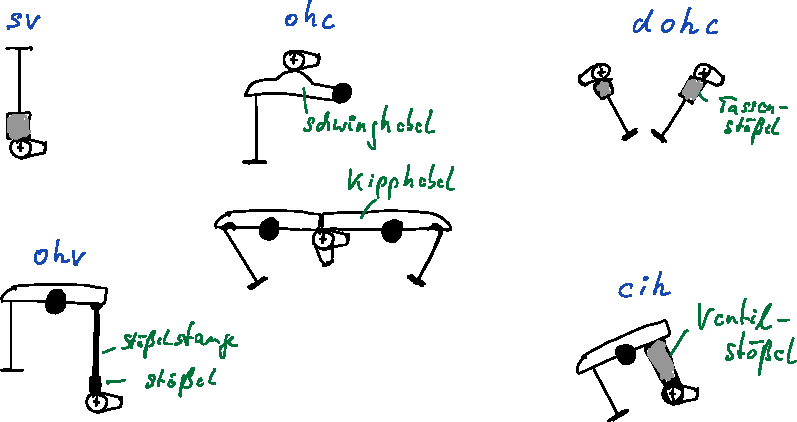
\includegraphics[width=0.6\textwidth]{images/Skizze/01_Anordnung-der-Nockenwelle_Skizze.pdf}
\caption{Anordnung der Nockenwelle}
%\label{fig:}%% anpassen
\end{figure}

\subsection{sv-Motor}\label{sv-motor}

\begin{itemize}
\item
  >>side valves<< seitlich stehende Ventile
\item
  untengesteuerter Motor
\item
  unten liegende Nockenwelle
\end{itemize}

\subsection{ohv-Motor}\label{ohv-motor}

\begin{itemize}
\item
  >>overhead valves<< hängende Ventile
\item
  obengesteuerter Motor
\item
  unten liegende Nockenwelle
\end{itemize}

\subsection{ohc-Motor}\label{ohc-motor}

\begin{itemize}
\item
  >>overhead camshaft<<
\item
  Nockenwelle über Zylinderkopf
\end{itemize}

\subsection{dohc-Motor}\label{dohc-motor}

\begin{itemize}
\item
  >>double overhead camshaft<<
\item
  zwei Nockenwellen über Zylinderkopf
\end{itemize}

\subsection{cih-Motor}\label{cih-motor}

\begin{itemize}
\item
  >>camshaft in head<<
\item
  Nockenwelle im Zylinderkopf
\end{itemize}

\section{Arten von
Nockenwellenantriebe}\label{arten-von-nockenwellenantriebe}

Fachbuch (\textcite{brand:2020:fachkundeKfz} S. 247)

\begin{enumerate}
\item
  Steuerkette
\item
  Zahnriemen
\item
  Königswelle
\item
  Stirnräder
\item
  Schubstangenmotoren
\end{enumerate}

\section{Nenne Zahnriemen Merkmale (trocken
laufend)}\label{nenne-zahnriemen-merkmale-trocken-laufend}

Fachbuch (\textcite{brand:2020:fachkundeKfz} S. 247)

\begin{itemize}
\item
  geringe Masse
\item
  geräuscharmer Lauf
\item
  begrenzte Standzeit, begrenzte Belastbarkeit
\item
  Unterliegen einem Wartungsintervall
\item
  braucht keine Schmierung
\item
  kostengünstig in der Produktion
\item
  Chemisch sensibel
\end{itemize}

\section{Ölbadzahnriemen Eigenschaften (nass
laufend)}\label{oelbadzahnriemen-eigenschaften-nass-laufend}

\begin{itemize}
\item
  mit Öl geschmierter Lauf
\item
  geringere Geräuschentwicklung
\item
  geringere Reibung ($20~\%$ weniger als Steuerkette)
\end{itemize}

\textbf{Ziel:}

\begin{itemize}
\item
  Kontaktflächen der beweglichen Teile reduzieren $\to$ Emissionen
\item
  Thermomanagement: Betriebstemperatur lange halten (BMW)
\end{itemize}

\section{Steuerkette Merkmale}\label{steuerkette-merkmale}

\begin{enumerate}
\item
  Große Kräfte übertragen
\item
  eigentlich wartungsarm, aus praktischer Sicht leider problembehaftet
\item
  teuer in Konstruktion
\item
  Steuerkette gilt als lauter
\item
  größere Masse als ein Riemen
\end{enumerate}

\section{Stirnradantrieb}\label{stirnradantrieb}

\begin{itemize}
\item
  Große Kräfte übertragen
\item
  wartungsfrei
\item
  schmale Bauform
\item
  teuer in Konstruktion
\item
  Dauerläufer (nicht problembehaftet)
\end{itemize}

\section{Königswelle}\label{koenigswelle}

\begin{itemize}
\item
  wartungsfrei
\item
  leicht, weil hohl gebohrt, Hohlröhre
\item
  kleine Kräfte übertragen
\item
  teuer in Konstruktion und Herstellung
\end{itemize}

\section{Unterschied - Steuern und
Regeln}\label{unterschied-steuern-und-regeln}

\textbf{Steuern} Soll-Ist-Vergleich

\begin{enumerate}
\def\labelenumi{\alph{enumi}.}
\setcounter{enumi}{25}
\item
  B. \emph{Steuerkette}: Markierung soll auf OT stehen, alles in
  Ordnung, wenn nicht, dann defekt.
\end{enumerate}

\textbf{Regeln} Soll-Ist-Vergleich mit der Option des Eingriffs

\begin{enumerate}
\def\labelenumi{\alph{enumi}.}
\setcounter{enumi}{25}
\item
  B. Steuerrad Kapitän, \emph{ABS Regelkreis}: SG erfasst
  Drehzahlsignal, Drehen alle Räder gleich schnell, alles okay. Dreht
  ein Rad schneller $\to$ aktiver Eingriff ins System.
\end{enumerate}

\section{Nockenwellen -
Herstellungsmöglichkeiten}\label{nockenwellen-herstellungsmoeglichkeiten}

\subsection{Gegossene Nockenwelle}\label{gegossene-nockenwelle}

\begin{itemize}
\item
  muss nachgearbeitet werden, Lagerstellen, partiell gehärtet
\item
  biegsam, flexibles Bauteil (Gusseisen mit Lamellen- o. Kugelgrafit)
\item
  \emph{Vorteil} kostengünstig in der Herstellung, weniger
  problembehaftet
\end{itemize}

(\emph{Kaltverformen} je härter ein Material, um zu spröder.)

\subsection{Gebaute Nockenwelle}\label{gebaute-nockenwelle}

\begin{itemize}
\item
  zwei unterschiedliche Materialien,
\item
  Nocken (aus Einsatz-, Vergütungs- o. Nitrierstahl) auf ein Stahlrohr
  geschrumpft
\item
  \emph{Problem} Nocken können sich verdrehen
\item
  \emph{Vorteil} Gewichtsreduzierung, Nocken ist belastbarer
\item
  \emph{Nachteil} Aufwand
\item
  Material V4A (hohl gebohrt)
\end{itemize}

\section{Nockenformen}\label{nockenformen}

Fachbuch (\textcite{brand:2020:fachkundeKfz} S. 246)

\begin{figure}[!ht]% hier: !ht
\centering
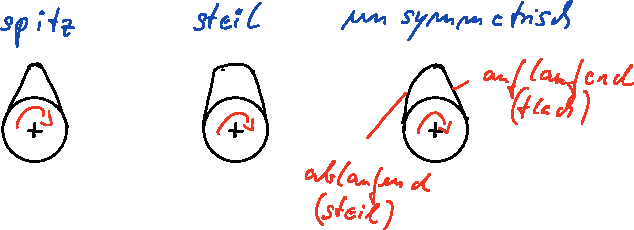
\includegraphics[width=0.6\textwidth]{images/Skizze/02_Nockenformen_Skizze.pdf}
\caption{Nockenformen}
%\label{fig:}%% anpassen
\end{figure}

\subsection{spitzer Nocken (tagenden
Nocken)}\label{spitzer-nocken-tagenden-nocken}

\begin{itemize}
\item
  langsames Öffnen / Schließen der Ventile
\item
  kurze Zeit voll geöffnet\\
\item
  geringe Füllung
\item
  stabiler Leerlauf
\item
  weicher und komfortorientierte Drehzahlbereich
\item
  nicht als hochdrehender, hochbelasteter Motor geeignet
\end{itemize}

\subsection{steiler Nocken (scharfer Nocken, Kreisbogen
Nocken)}\label{steiler-nocken-scharfer-nocken-kreisbogen-nocken}

\begin{itemize}
\item
  schnelles Öffnen / Schließen der Ventile
\item
  bleibt längere Zeit voll geöffnet
\item
  hoher Füllungsgrad, bei hohen Drehzahlen
\item
  im Leerlauf teilweise unrunder Lauf, da >>inneres AGR<< entstehen kann
  (große Ventilüberschneidung $\to$ Abgase in Ansaugtrakt) Abhilfe:
  Leerlaufdrehzahl erhöhen (750 $\to$ 950 U/min.)
\item
  Leistungsmotoren, hohe Drehzahlen
\end{itemize}

\subsection{unsymmetrischer Nocken}\label{unsymmetrischer-nocken}

\begin{itemize}
\item
  \emph{flach} langsameres öffnen der Ventile
\item
  \emph{steil} schnelles schließen der Ventile
\item
  längeres offen halten der Ventile
\item
  vereinigt beide Varianten
\end{itemize}

(\emph{Ziel bei hohen Drehzahlen}: Ventile schnell öffnen (Nocken) /
schließen (Ventilfeder) $\to$ gute Füllung, hohen Wirkungsgrad
erreichen.)

\section{Arten von
Ventilbetätigung}\label{arten-von-ventilbetaetigung}

Fachbuch (\textcite{brand:2020:fachkundeKfz} S. 247, 242)

\begin{figure}[!ht]% hier: !ht
\centering
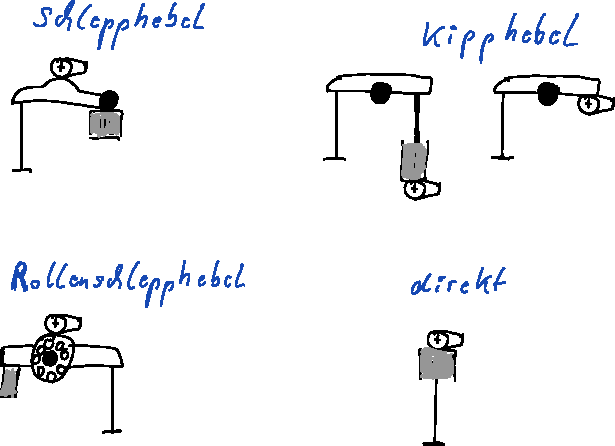
\includegraphics[width=0.6\textwidth]{images/Skizze/03_Arten-von-Ventilbetaetigung_Skizze.pdf}
\caption{Arten von Ventilbetätigung}
%\label{fig:}%% anpassen
\end{figure}

\subsection{Rollenschlepphebel, Schlepphebel,
Schwinghebel}\label{rollenschlepphebel-schlepphebel-schwinghebel}

\begin{itemize}
\item
  einarmige Hebel
\item
  geringe Reibung zwischen Nocken und Schlepphebel durch Nockenrolle
  (nadelgelagert)
\end{itemize}

\subsection{Kipphebel}\label{kipphebel}

zweiarmige Hebel

\subsection{direkt}\label{direkt}

Nockenwelle - Hydrostößel - Ventil

\section{Welche Beanspruchung ist das Ventil
ausgesetzt?}\label{welche-beanspruchung-ist-das-ventil-ausgesetzt}

\subsection{Mechanische Beanspruchung des
Ventils}\label{mechanische-beanspruchung-des-ventils}

\begin{itemize}
\item
  Ziehen (Ventilfeder, schließen, Ventilsitz)
\item
  Druck (Nocken, öffnen)
\item
  Torsion (verdrehen)
\item
  Biegen
\end{itemize}

\subsection{Chemische Beanspruchung}\label{chemische-beanspruchung}

Schwefel im Kraftstoff $\to$ Korrosion

\subsection{Thermische Belastung}\label{thermische-belastung}

Auslassventil bis $900^\circ\text{C}$

\section{Ventilspielausgleich}\label{ventilspielausgleich}

\textbf{Wofür?} Temperaturänderung (Motor Kaltstart, temperaturbedingte
Längenänderung des Ventils ausgleichen)

\textbf{Zu kleines Ventilspiel} (Nachteile)

\begin{itemize}
\item
  Ventil öffnet früher und schließt später
\item
  Ventil ist länger auf
\item
  kann dadurch nicht genügend Wärme abgeben über Ventilsitz
\item
  Ventilteller wird immer weiter einer höheren thermischen Belastung
  unterzogen und dadurch erhöhter Verschleiß
\item
  Am Ende ist das Ventil einer Hochtemperaturkorrosion unterworfen
  (Verbranntes Ventil)
\end{itemize}

\textbf{zu großes Ventilspiel} (Nachteile)

\begin{itemize}
\item
  Ventil öffnet zu spät, geht nicht ganz auf und schließt zu früh
\item
  Ventil ist kürzer auf
\item
  Klappergeräusche und erhöhter Verschleiß, \emph{Warum?} durch großes
  Ventilspiel, liegt nicht am Nockengrundkreis auf (Nocken schlägt auf
  Ventil)
\item
  Hieraus können folgen: schlechte Zylinderfüllung und die maximale
  erreichbare Leistung sinkt
\end{itemize}

\subsection{definiertes Ventilspiel}\label{definiertes-ventilspiel}

Wartung notwendig

\subsection{Hydraulischer
Ventilspielausgleich}\label{hydraulischer-ventilspielausgleich}

\textbf{ablaufender Nocken} (ohne Belastung)

\begin{itemize}
\item
  Entspannung des Systems
\item
  Spielausgleichsfeder drückt Druckbolzen nach oben bis Stößel am Nocken
  anliegt
\item
  Kugelventil öffnet sich, Raumvergrößerung im Arbeitsraum (Unterdruck)
\item
  Durch den Systemdruck strömt frisches Öl von außen ein und der
  Arbeitsraum wird befüllt
\end{itemize}

\textbf{auflaufender Nocken} (mit Belastung)

\begin{itemize}
\item
  Kugelventil schließt sich, es baut sich Druck im System auf
\item
  durch die Inkompressibilität von Flüssigkeiten $\to$ starre
  Verbindung
\item
  Nocken wird auf den Stößel auflaufen können, ohne Spiel zu haben und
  das Ventil betätigen
\item
  \emph{Warum Ringspalt?} (Wärmeausdehnung des Öls ausgleichen)
\item
  dadurch wird >>Öl<< durch den kleinen Ringspalt gepresst (definierte
  Ölmenge)
\end{itemize}

\textbf{Bemerkung} Wärmeeintrag: >>Je wärmer das Öl, umso
dünnflüssiger.<< Erfordert die \emph{richtige Öl-Viskosität}
(Zähflüssigkeit, Temperaturabhängig, Fließverhalten), sind an diese
Ringspalte angepasst.

\emph{falsche Öl-Viskosität} ein Klappern oder Aufpumpen der Hydrostößel
$\to$ darf nicht sein sonst Thermische Überlast,
Hochtemperaturkorrosion $\to$ verbrannte Ventile

Fachbuch (\textcite{brand:2020:fachkundeKfz} S. 245)

\begin{figure}[!ht]% hier: !ht
\centering
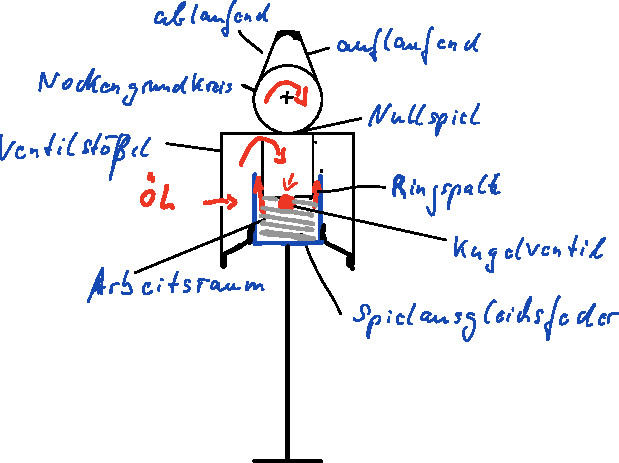
\includegraphics[width=0.6\textwidth]{images/Skizze/04_Ventilspielausgleich_Skizze.pdf}
\caption{Ventilspielausgleich}
%\label{fig:}%% anpassen
\end{figure}

\section{Drehzahlverhältnis zwischen Kurbelwelle zu
Nockenwelle?}\label{drehzahlverhaeltnis-zwischen-kurbelwelle-zu-nockenwelle}

2:1

\section{Was steuert die
Motorsteuerung?}\label{was-steuert-die-motorsteuerung}

Den Zeitpunkt und die Dauer des Ansaugens der Frischgase und den
Zeitpunkt und die Dauer des Ausstoßes der Abgase.

Öffnen und Schließen der Ventile.

\textbf{Voraussetzung}

\begin{enumerate}
\item
  Einspritzung des Kraftstoffs (Energieträger)
\item
  Eine Zündung, die diese Energie, gebunden im Kraftstoff, in chemische
  Energie, in Wärmeenergie umwandelt (Wärmekraftmaschine)
\end{enumerate}

Druck wird über eine Fläche in Kraft und Drehmoment übertragen, an die
Kurbelwelle übergeben, läuft durch das Getriebe - Achswellen - Reifen
auf die Straße und wir haben Vortrieb.

\section{Dreiventiltechnik mit zwei
Zündkerzen}\label{dreiventiltechnik-mit-zwei-zuendkerzen}

Fachbuch (\textcite{brand:2020:fachkundeKfz} S. 243)

Fachbuch (\textcite{respondeck:2019:servicetechniker} S. 142)

\subsection{Zusammenfassung}\label{zusammenfassung}

\begin{figure}[!ht]% hier: !ht
\centering
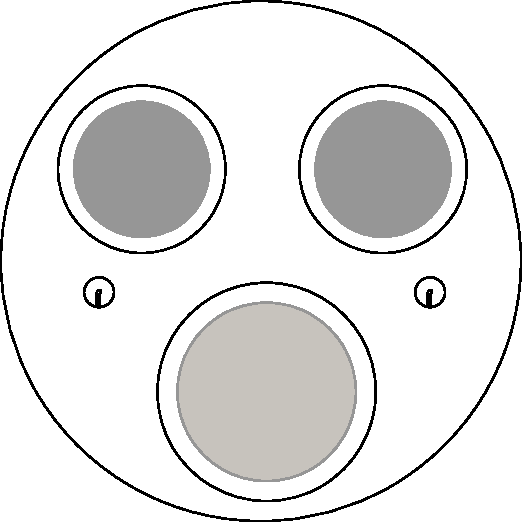
\includegraphics[width=0.2\textwidth]{images/Skizze/05_Dreiventiltechnik_Skizze.pdf}
\caption{Dreiventiltechnik}
%\label{fig:}%% anpassen
\end{figure}

Wir haben bei \textbf{drei Ventilen} einen großen Ein- und
Auslassquerschnitt.

Durch die Anordnung ist eine Unterbringung von \textbf{zwei Zündkerzen}
möglich, sodass zwei Zündkerzen in der Nähe der Zylinderwand entstehen
in deren Umgebung zwei Flammfronten. Somit kann bereits
niedergeschlagener Kraftstoff noch verdampfen und verbrannt werden.

Durch zwei Zündkerzen findet die Verbrennung schneller statt. Dadurch
wird der maximale Kolbendruck früher erreicht und ein hohes Drehmoment
erreicht. Wir nähern uns einer Gleichdruckverbrennung (Isobar).

\textbf{Klopfneigung} wird durch zwei Zündkerzen verringert. Da
geringere Wärmeeintrag in die noch nicht verbrannten Gase stattfindet.

\textbf{Abgastemperatur} ist niedriger, dadurch geringerer NOx-Ausstoß
trotz geringer HC und CO-Werte.

Dank nur \textbf{einem Abgasrohr} geringere Wärmeverluste. >>light off
point<< des Katalysators wird schneller erreicht.

\subsection{Warum sind das zwei Einlassventile und ein
Auslassventil?}\label{warum-sind-das-zwei-einlassventile-und-ein-auslassventil}

\textbf{Vorteil}

\begin{itemize}
\item
  kleine Massen
\item
  zwei kleine Ventile $\to$ große Einlassquerschnitte
\item
  höhere Drehzahlen
\item
  gute Füllung und Zylinderspülung
\end{itemize}

\textbf{Nachteil}

\begin{itemize}
\item
  mehr Teile $\to$ größere Reibungsverluste
\item
  Verschleiß und Ausfallwahrscheinlichkeiten
\end{itemize}

\textbf{Ein großes Ventil} hat eine Massenträgheit.

\begin{itemize}
\item
  Masse in Ruhelage (Ventil offen), Losbrechmoment~ $\to$ höchste
  Kraft, Masse in Bewegung (Federkraft: Ventil schließen)
\item
  Ansaugventil möglichst lange offen lassen (Kolben und Ventil kommen
  sich sehr nahe)
\item
  \emph{Ziel:} bestimmte Drehzahl erreichen (Wie schnell kann dieser
  Wechsel vollzogen werden?)
\end{itemize}

\subsection{Zylinderspülung bei
Ventilüberschneidung}\label{zylinderspuelung-bei-ventilueberschneidung}

Mit dem Ausstoß der Abgase ziehen wir einen kleinen definierten
Frischgasanteil mit, um den Zylinder zu spülen und möglichst wenig
inertes Gas (AGR) zu gewährleisten.

\subsection{Nachladeeffekt beim
Ansaugen}\label{nachladeeffekt-beim-ansaugen}

Einlassventile werden erst nach Durchschreiten des unteren Totpunktes
geschlossen. Frischgase strömen trotz aufwärtsgehendem Kolben in den
Zylinder nach. Die Kinetische Energie der einströmenden Frischgase ist
größer, als die Druckzunahme durch aufwärts gehenden Kolben.

\subsection{Warum zwei Zündkerzen?}\label{warum-zwei-zuendkerzen}

Zündkerze ist in der Nähe der Zylinderwand, zwei Flammenfronten
entstehen.

\begin{enumerate}
\item
  \textbf{Vollständige Verbrennung}

  \begin{itemize}
  \item
    niedergeschlagener Kraftstoff verdampft (an Zylinderwandung und
    Feuersteg) und der Verbrennung zugeführt
  \end{itemize}
\item
  \textbf{schnellerer Verbrennungsablauf}

  \begin{itemize}
  \item
    Schnelleres erreichen des maximalen Verbrennungsdruckes. Die
    Temperatur kann schneller konstant gehalten bzw. in Druck
    umgewandelt und über die Fläche des Kolbens in Kraft und Drehmoment
    auf die Kurbelwelle übertragen werden.
  \item
    Drehmoment = Kraft (max. Kolbendruck) x Hebelarm (90° stehende
    Kurbelwellenzapfen = Hebelarm am größten)
  \end{itemize}
\end{enumerate}

\subsection{Innermotorisch entstehen geringere
Schadstoffe}\label{innermotorisch-entstehen-geringere-schadstoffe}

\begin{enumerate}
\item
  \textbf{HC} geringer Ausstoß unverbrannter Kohlenwasserstoffe, durch
  weniger niedergeschlagener Kraftstoff
\item
  \textbf{CO} geringer, durch vollständige Verbrennung
\item
  \textbf{NOx} ist reduziert, durch schnelleren Verbrennungsablauf
  $\to$ zwei Zündkerzen, Abgastemperatur ist niedriger
\end{enumerate}

\subsection{Wann entsteht NOx?}\label{wann-entsteht-nox}

Durch hoher Druck und hohe Temperatur.

\subsection{Zusammenhang zwischen HC und CO
vs.~NOx}\label{zusammenhang-zwischen-hc-und-co-vs.-nox}

Es gibt zwei Zündgrenzen >>fett<< und >>mager<<.

\begin{enumerate}
\item
  \textbf{HC und CO} entsteht durch unvollständige fette Verbrennung

  \begin{itemize}
  \item
    Senken: durch Abmagern
  \item
    Verbrennungsspitzentemperatur: geringer
  \end{itemize}
\item
  \textbf{NOx} entsteht durch magere Verbrennung

  \begin{itemize}
  \item
    Senken: durch anfetten
  \item
    Verbrennungsspitzentemperatur: ansteigen
  \end{itemize}
\end{enumerate}

\subsection{Schadstoffe}\label{schadstoffe}

\begin{enumerate}
\item
  \textbf{HC} unverbrannte Kohlenwasserstoffe

  \begin{itemize}
  \item
    Verdampft am Ende der Verbrennung und wird dem Abgas zugeführt
  \end{itemize}
\item
  \textbf{CO} Kohlenmonoxid

  \begin{itemize}
  \item
    schwerer als Luft (Grube), bindet Hämoglobin im Blut
  \item
    keine vollständige Verbrennung
  \end{itemize}
\item
  \textbf{NOx} Stickoxide
\end{enumerate}

\subsection{Was ist AGR?}\label{was-ist-agr}

Platzhalter Gas (inertes Gas) nimmt nicht an der Verbrennung teil, soll
den Umgebungssauerstoff fernhalten

AGR-Rate ist am größten in Teillast (80 Km/h auf der Landstraße)

Ziel: Aus großen Motor $\to$ kleinen Motor machen, viel Abgas und
geringe Menge Kraftstoff einspritzen

\emph{Problem} >>Luftmenge ist da und kein Kraftstoff Einspritzen<<
$\to$ magere Verbrennung $\to$ thermische Belastung und Anstieg NOx

\emph{Luftmassenmesser} misst angesaugte Luftmasse und Sauerstoffgehalt
$\to$ AGR-Rate $\to$ Kraftstoffmenge berechnen

Ziel: homogen - Magerbetrieb (über den kompletten Zylinder)

\subsection{Wie entsteht Ruß?}\label{wie-entsteht-russ}

Kraftstoff wird an heißen Luft eingespritzt, zündfähiges
Kraftstoff-Luft-Gemisch bildet sich

\emph{einzelne Kraftstofftröpfchen}

\begin{itemize}
\item
  fangen von außen an zu verdunsten, entzünden, Verbrennung ist zu kurz
  (nicht vollständig)
\item
  innen: Verbrennung von Kohlenwasserstoff ohne Sauerstoff
\end{itemize}

\subsection{Was fördert die
Klopfneigung?}\label{was-foerdert-die-klopfneigung}

Unkontrollierte, unerwünschte Verbrennung (Glühzündung, klingende,
klopfende Verbrennung)

entzündet sich selbst an etwas glühenden, z. B. Ölkohle, Masseelektrode
(Zündkerze)

Wärme braucht Zeit zum Wirken.

\begin{enumerate}
\item
  \textbf{Wärmeeintrag gering:} geringe Klopfneigung, geringe thermische
  Belastung, schneller Verbrennungsablauf
\item
  \textbf{Wärmeeintrag hoch:} klopfende Verbrennung
\end{enumerate}

\subsection{Ein Auslassventil - ein
Abgasrohr}\label{ein-auslassventil-ein-abgasrohr}

Abgas verliert weniger Wärmeenergie.

\begin{enumerate}
\item
  ab ca. 450~°C >>light off point<< des Katalysators: min. $50~\%$ der
  Abgase konvertiert in nicht Schadstoffen
\item
  ab ca. 650 °C altert der Katalysator exponentiell und thermische
  Belastung
\end{enumerate}

\textbf{Thermodynamik - warme Luft strömt} schneller, weniger Rückstau.

Das unter Druck stehende Abgas verlässt den Zylinder mit Überschall
(Auspuffgeräusch). \textbf{Schallgeschwindigkeit} ca. 343 m/s (z. B.
Blitz $\to$ Donner, drei Sekunden zählen $\to$ ca. 1 km Entfernung)

\chapter{03-Fuellungsoptimierung-I}
%%ju 31-Dez-22 03-Fuellungsoptimierung-I.tex
\section{Downsizing (Prüfung)}\label{downsizing-pruefung}

Verkleinerung der Motoren (Hubraum und Zylinderzahl) bei gleicher
Leistung.

\section{LSPI - Low
Speed-Pre-Ignition}\label{lspi-low-speed-pre-ignition}

LSPI = vorzeitige Zündung, betrifft hoch aufgeladene Downsizing Motoren
\footnote{\url{https://www.autobild.de/artikel/lspi-vorzeitige-zuendung-16385077.html}}

\begin{itemize}
\item
  \textbf{Turbo aufgeladene Motoren}

  \begin{itemize}
  \item
    geringes Verdichtungsverhältnis (7-8:1)
  \item
    vor verdichtete Luft wird in den Zylinder eingeblasen und verdichtet
  \item
    Ladedruckregelung (Lastwunsch)
  \item
    vorgewärmte Luft (Ladeluftkühlung)
  \end{itemize}
\item
  vs.~\textbf{hoch verdichtete Saugmotoren}

  \begin{itemize}
  \item
    hohes Verdichtungsverhältnis (10-11:1), endet bei Klopfgrenze
  \end{itemize}
\end{itemize}

\textbf{Zwei Zündquellen, Ursache für die Selbstentzündung}

\begin{enumerate}
\item
  Niedergeschlagen Kraftstoff in Verbindung mit sehr niedrig Viskoses Öl

  \begin{itemize}
  \item
    $\to$ ein brennbares Gemisch entsteht, mit einer nicht ganz
    bekannten Selbstentzündungstemperatur
  \end{itemize}
\item
  Ölkohlerückstände (Kraftstoffreste) im Bereich der Einspritzdüsen
\end{enumerate}

Durch eine überhohe Verdichtung $\to$ steigt Verdichtungsenddruck und
damit Verdichtungstemperatur $\to$ dadurch hohe thermische Belastung.
Die Folge ist ein kapitaler Motorschaden.

\textbf{Körnerschlag} \footnote{\url{https://cdn.germanscooterforum.de/monthly_05_2009/post-24449-1241606436.jpg}}
Kolbenschäden $\to$ es entsteht eine Druckspritze bevor der Kolben OT
erreicht, eine zweite Flammenfront entsteht, wenn jetzt zwei
Flammfronten aufeinandertreffen, entstehen sehr hohe Druckspitzen, auch
wenn der Kolben nach UT geht.

\textbf{Kavitation} \footnote{\url{https://prozesstechnik.industrie.de/wp-content/uploads/4/0/40278086.jpg}}
Dampfblasenbildung \footnote{\url{https://www.youtube.com/watch?v=SEGTFbZ5RJ8}}
z. B. Bootsschraube saugt Flüssigkeiten an, Druck fällt ab durch
Unterdruck, wenn jetzt die Gasblasen implodieren, entstehen sog.
Mikrojets $\to$ Druckspitzen.

\section{Vorteile von Downsizing
Motoren}\label{vorteile-von-downsizing-motoren}

\begin{enumerate}
\item
  Geringere Pumpverluste (2 l vs.~1,2 l bei gleicher Leistung 150 PS)
\item
  geringere Reibungsverluste aufgrund der geringeren Größe
\item
  weniger Wärmeübertrag von Gasen zur Zylinderwandung
\end{enumerate}

\section{Mehrventiltechnik}\label{mehrventiltechnik}

Fachbuch (\textcite{respondeck:2019:servicetechniker} S. 141)

Um die Zylinderfüllung zu verbessern, werden drei oder mehr Ventile pro
Zylinder in Verbrennungsmotoren eingesetzt.

\textbf{Ziele von Mehrventiltechnik}

\begin{itemize}
\item
  Öffnungsquerschnitt der Ventile vergrößern, ohne die
  Drehzahlfestigkeit durch größere und damit trägere Ventile (mehr
  Masse) zu mindern.
\end{itemize}

\textbf{Vor- und Nachteile von Mehrventiltechnik}

\begin{itemize}
\item
  bessere Zylinderfüllung
\item
  Drehzahlfest
\item
  innere Reibung steigt
\item
  Abgaswärmeentzug

  \begin{itemize}
  \item
    Der Katalysator kommt schlechter auf Betriebstemperatur, da sich die
    Abgase an den Abgasrohren abkühlen können.
  \item
    Je mehr Auslassventile vorhanden sind, desto größer ist die
    Oberfläche der Abgasrohre und desto mehr kühlen die Abgase aus.
  \end{itemize}
\end{itemize}

Honda NR 750 - Ovalkolben \footnote{\url{https://de.wikipedia.org/wiki/Honda_NR_750}}

\textbf{Dreiventiltechnik} (Vorteile)

\begin{itemize}
\item
  Verbrennungsdruck steigt (kürzere Flammwege)
\item
  geringere Klopfneigung (weniger Zeit zur Gemischerwärmung vor
  Verbrennungsbeginn)
\item
  Ausstoß unverbrannter Kohlenwasserstoffe verringert sich (Zündkerze
  ist in der Nähe der Zylinderwand, wo das Kondensat lagert)
\item
  geringere NOx
\end{itemize}

Vgl. Kapitel >>\emph{Motorsteuerung / Dreiventiltechnik mit zwei
Zündkerzen}<<

\section{Nockenwellenverstellung - variable
Steuerzeiten}\label{nockenwellenverstellung-variable-steuerzeiten}

Fachbuch (\textcite{brand:2020:fachkundeKfz} S. 249)

Verdrehen der Einlassnockenwelle bzw. der Ein- und Auslassnockenwelle,
abhängig von der Motordrehzahl, Motorlast und Temperatur. Hierdurch
lässt sich die \emph{Länge der Ventilüberschneidung} anpassen.

\textbf{Warum machen wir eine Nockenwellenverstellung?} (Vorteile)

\begin{enumerate}
\item
  Optimale Zylinderfüllung in den unterschiedlichen Last- und
  Drehzahlbereichen zu ermöglichen
\item
  inneres AGR
\end{enumerate}

\textbf{Ziele der Nockenwellenverstellung}

\begin{itemize}
\item
  Wann das Ventil öffnet und schließt zu beeinflussen (variabel)
\item
  bei gleichbleibenden Nocken, Dauer und Öffnungswinkel (Hub) ändern
  sich nicht
\item
  Verdrehrichtung der Nockenwelle: Früh, Spät
\end{itemize}

\textbf{Verstellung der Einlassnockenwelle in Abhängigkeit vom
Betriebszustand}

\begin{table}[!ht]% hier: !ht 
\centering 
	\caption{}% \label{tab:}%% anpassen 
\begin{tabular}{@{}llll@{}}
\hline
\textbf{Betriebszustand} & \textbf{Leerlauf} & \textbf{Teillast} &
\textbf{Volllast} \\
\hline
Verstellrichtung NW & Spät & Früh & Spät \\
Ventilüberschneidung & klein & groß & klein \\
Abgas & CO sinkt & NOx sinkt & \\
EV schließt & weit nach UT & kurz nach UT & weit nach UT \\
\hline
\end{tabular} 
\end{table}

Merkmale (Vgl. Tabelle Verstellung der Einlassnockenwelle in
Abhängigkeit vom Betriebszustand)

\begin{itemize}
\item
  \textbf{Leerlauf} Kein Überströmen von Frischgasen und Abgasen,
  besserer Verbrennungsverlauf
\item
  \textbf{Teillast} Abgase strömen in den Einlasskanal und werden mit
  den Frischgasen angesaugt. Temperatur sinkt, NOx-Anteil sinkt
\item
  \textbf{Volllast} \emph{Nachladeeffekt} Frischgase strömen trotz
  aufwärts gehenden Kolben in den Zylinder nach
\end{itemize}

\textbf{Ausgangspunkt} $\to$ 90er-Jahre, erste Form des AGR (inneres
AGR), Drei-Wege-Katalysator, Ottomotor, Euro 2, Teillast (höchste
AGR-Rate, 80 km/h auf der Landstraße, keine Lastabfrage,
Spritspareffekt, NOx-Anteil senken)

\subsection{VarioCam - Verstellbarer Kettenspanner (Audi,
VW)}\label{variocam-verstellbarer-kettenspanner-audi-vw}

$\to$ Verändern der Ventilöffnungszeit der Einlassnockenwelle

\textbf{Wie?} Vgl. Tabelle Verstellung der Einlassnockenwelle in
Abhängigkeit vom Betriebszustand

\begin{itemize}
\item
  KW treibt Auslass-NW an und diese über einer Kette die Einlass-NW
\item
  \textbf{Kettenspanner} spannt \textbf{Kette nach oben} (federbelastet)
\item
  \textbf{NW} dreht sich \textbf{gegen UZS} (Uhrzeigersinn) in
  \textbf{Verstellposition} >>spät<< (Ausgangslage, Ventilüberschneidung
  klein)
\item
  SG bestromt Magnetventil, Motoröl fließt in Kettenspanner.
\item
  \textbf{Kettenspanner} spannt \textbf{Kette nach unten}
  (Hydraulikzylinder)
\item
  \textbf{NW} dreht sich \textbf{im UZS} in \textbf{Verstellposition}
  >>früh<<, (Ventilüberschneidung groß)
\end{itemize}

\subsection{Vanos - Variable Nockenwellensteuerung
(BMW)}\label{vanos-variable-nockenwellensteuerung-bmw}

\textbf{Wie?}

\begin{itemize}
\item
  \textbf{Nockenwellenrad und Nockenwelle} sind über ein \textbf{steiles
  Gewinde} miteinander verbunden.
\item
  \emph{Grundposition} NW steht in \textbf{Verstellposition} >>spät<<
\item
  SG bestromt ein Magnetventil (4/2-Wegeventil) $\to$ gibt den
  \textbf{Ölzufluss} zum Frühkanal frei
\item
  NW verdreht sich gegen Uhrzeigersinn in \textbf{Verstellposition}
  >>früh<<
\item
  Durch wechselseitigen Druckaufbau lässt sich die Position der
  Verstelleinheit halten.
\end{itemize}

\subsection{Flügelzellenversteller
(Mercedes)}\label{fluegelzellenversteller-mercedes}

$\to$ Verändern der Steuerzeiten

\textbf{Wie?}

\begin{itemize}
\item
  \textbf{Innenrotor} (fest mit NW) \textbf{und Außenrotor} (fest mit
  Kettenrad)
\item
  SG bestromt \textbf{Magnetventil} $\to$ die \textbf{Ölräume}
  zwischen den Rotorblättern können wechselseitig mit Öl befüllt werden
\item
  Die Kraftübertragung vom Nockenwellenrad auf die NW erfolgt immer über
  das Öl.
\item
  wird Ölraum rechts vom Innenrotorblatt mit Öl befüllt, kommt es zu
  einer \textbf{Verdrehung der NW gegen UZS} (Uhrzeigersinn) in Richtung
  >>spät<<
\item
  wird Ölraum links vom Innenrotorblatt mit Öl befüllt, kommt es zu
  einer \textbf{Verdrehung der NW im UZS} in Richtung >>früh<<
\item
  Durch wechselseitigen Druckaufbau lässt sich die Position der
  Verstelleinheit halten.
\end{itemize}

\section{Variabler Ventiltrieb}\label{variabler-ventiltrieb}

\subsection{Stufenweise variabler
Ventiltrieb}\label{stufenweise-variabler-ventiltrieb}

\textbf{Vorteile}

Bessere Zylinderfüllung durch zwei unterschiedliche Nockenprofile

\begin{itemize}
\item
  \emph{obere Drehzahlbereich} $\to$ steiler Nocken

  \begin{itemize}
  \item
    schnelles Öffnen, lange Öffnungsdauer, schnelles Schließen
  \end{itemize}
\item
  \emph{untere Drehzahlbereich} $\to$ spitzer Nocken

  \begin{itemize}
  \item
    Verhinderung von ungewollter Abgasrückführung durch zu lange
    Ventilüberschneidung
  \end{itemize}
\end{itemize}

\subsubsection{VTEC - Variable Valve Timing and Lift Electronic Control
(Honda)}\label{vtec-variable-valve-timing-and-lift-electronic-control-honda}

$\to$ Verändern von Ventilhub und Ventilöffnungszeit

\textbf{Wie?}

\begin{itemize}
\item
  Verstelleinheit liegt in den Schlepphebeln
\item
  \textbf{Umschaltung} zwischen dem Nockenprofilen erfolgt durch
  \textbf{Verblocken der Schlepphebel}
\item
  \textbf{Schlepphebel entriegelt}

  \begin{itemize}
  \item
    Die beiden äußeren Nocken öffnen mithilfe der äußeren Schlepphebel
    die Ventile.
  \item
    \textbf{Spitzer Nocken}

    \begin{itemize}
    \item
      kleiner Ventilhub
    \item
      kurze Ventilöffnungszeit
    \item
      \emph{niedrige Drehzahlen}
    \end{itemize}
  \end{itemize}
\item
  SG bestromt Elektromagnet, \textbf{Öldruck} verschiebt die
  \textbf{Sperrschieber} und verblockt die Schlepphebel untereinander.
\item
  \textbf{Schlepphebel verriegelt}

  \begin{itemize}
  \item
    wenn der steile Nocken auf den mittleren Schlepphebel aufläuft,
    nimmt dieser die beiden äußeren Schlepphebel mit und diese öffnen
    die Ventile.
  \item
    \textbf{Steiler Nocken}

    \begin{itemize}
    \item
      großer Ventilhub
    \item
      lange Ventilöffnungszeit
    \item
      \emph{hohe Drehzahlen}
    \end{itemize}
  \end{itemize}
\end{itemize}

\subsubsection{VarioCam Plus (Porsche)}\label{variocam-plus-porsche}

$\to$ Verändern von Ventilhub und Ventilöffnungswinkel

\textbf{Wie?}

\begin{itemize}
\item
  Verstelleinheit liegt im Tassenstößel
\item
  SG bestromt \textbf{Elektromagnet}, damit wird der
  \textbf{Tassenstößel mit Öldruck} gesteuert
\item
  Diese bestehen aus \textbf{zwei Stößeln}, die mithilfe eines
  \textbf{Bolzens} gegeneinander verriegelt werden können.
\item
  innere Stößel $\to$ kleinen Nocken
\item
  äußere Stößel $\to$ großen Nocken
\item
  \textbf{Stößel verriegelt} $\to$ große Ventilhub

  \begin{itemize}
  \item
    Innere und äußere Stößel wird durch einen Bolzen verriegelt
  \end{itemize}
\item
  \textbf{Stößel entriegelt} $\to$ kleiner Ventilhub

  \begin{itemize}
  \item
    sinkt der Öldruck, wird durch die Federkraft der Bolzen
    zurückgeschoben
  \end{itemize}
\end{itemize}

\subsubsection{Valvelift (Audi, +
Zylinderabschaltung)}\label{valvelift-audi-zylinderabschaltung}

\textbf{Wie?}

\begin{itemize}
\item
  Änderung des Nockenprofils durch Verschieben der Verstelleinheit
  (Nockenstück) auf der NW
\item
  SG bestromt \textbf{Elektromagnet} $\to$ \textbf{Metallstift} fährt
  aus \textbf{in eine Spiralnut} und verschiebt das \textbf{Nockenstück}
\item
  damit schalte ich zwischen \textbf{zwei Nockenprofilen} um
\item
  Arretierung des Nockenstücks erfolgt durch eine federbelastete Kugel.
\item
  \textbf{Zylinderabschaltung} (Teillast)

  \begin{itemize}
  \item
    Nockenprofil $\to$ Nockengrundkreis
  \item
    Die Ventile bleiben bei abgeschaltetem Zylinder geschlossen.
  \end{itemize}
\end{itemize}

\subsection{Stufenlos variabler
Ventiltrieb}\label{stufenlos-variabler-ventiltrieb}

\textbf{Vorteile}

$\to$ Verändern von Ventilhub in allen Drehzahlbereichen

\textbf{Ziel im unteren Drehzahlbereich}: Ein zündbares Gemisch zu
realisieren.

\textbf{Wie?}

\begin{itemize}
\item
  Durch geringe Ventilöffnung und damit Erhöhung der
  Strömungsgeschwindigkeit der Frischgase

  \begin{itemize}
  \item
    >>Venturi-Prinzip<< eine Verengung in einem Strömungskanal

    \begin{itemize}
    \item
      $\to$ höhere Strömungsgeschwindigkeit
    \item
      $\to$ bessere Verwirbelung
    \item
      $\to$ bessere Verteilung des Kraftstoff-Luftgemisches
    \end{itemize}
  \end{itemize}
\item
  Drosselklappe könnte wegfallen, wird aber weiterhin verbaut
\item
  \textbf{Wozu ist die Drosselklappe dann noch notwendig?}

  \begin{itemize}
  \item
    Schaltung des AGR (Abgasrückführung)

    \begin{itemize}
    \item
      Aufbau eines Druckgefälles/Druckdifferenz, durch Schließen der
      Drosselklappe wird ein Unterdruck erzeugt, was dazu führt, dass
      die Abgase in den Ansaugtrakt einströmen können
    \end{itemize}
  \end{itemize}
\item
  Notlauf
\end{itemize}

\subsubsection{Valvetronic}\label{valvetronic}

$\to$ Verändern von Ventilöffnungswinkel (Hub) und Ventilöffnungsdauer
(Nockenwellenverstellung)

\textbf{Wie?}

\begin{itemize}
\item
  SG verdreht mithilfe eines \textbf{Stellmotors} eine
  \textbf{Exzenterwelle} (Halbmondförmig)
\item
  Druck des Nockens wird zunächst auf einen \textbf{Zwischenhebel}
  übertragen
\item
  Der \textbf{Leerweg}, den der Zwischenhebel von der Betätigung durch
  den Nocken bis zur Übertragung auf das Ventil durchläuft, ist mittels
  einer Exzenterwelle einstellbar.
\item
  Je größer der Leerweg, desto kleiner der Ventilhub.
\item
  \textbf{Ventilhub} 0,3 mm und 9,85 mm
\end{itemize}

\subsubsection{Elektrohydraulischer Ventiltrieb
(MultiAir)}\label{elektrohydraulischer-ventiltrieb-multiair}

\textbf{Vorteil} Vollvariable Steuerzeiten

$\to$ stufenlose Veränderung von Ventilhub, Ventilöffnungsdauer und
die Anzahl der Ventilhübe der EV

\textbf{Wie?}

\begin{itemize}
\item
  auf der \textbf{Auslassnockenwelle} gibt es einen
  \textbf{Extranocken}, über Schlepphebel wird ein
  \textbf{Pumpenelement} betätigt

  \begin{itemize}
  \item
    $\to$ der erzeugt einen \textbf{Öldruck}, um die
    \textbf{Einlassseite} zu steuern,
  \end{itemize}
\item
  \textbf{Magnetventil geschlossen} Druck wird auf den Kolben
  übertragen, Ventil öffnen
\item
  \textbf{Magnetventil offen} Ventil schließen. Der Öldruck fließt in
  den Druckspeicher ab.
\item
  \emph{Vorteil \textbf{Druckspeicher}:} von der Nockenwelle
  unabhängiger Zeitpunkt, mit Öffnung eines Magnetventils (SG) ein
  Öldruck aus dem Druckspeicher nutzen, der das \textbf{Ventil
  öffnet/schließt}
\item
  \textbf{elektrohydraulisch-pneumatisch} (Ventile unabhängig von NW
  betätigen, noch nicht in der Großserie)
\item
  chinesische Hersteller Qoros und der schwedische
  Luxussportwagenhersteller Königsegg
\end{itemize}

\subsubsection{Elektromagnetischer Ventiltrieb (noch nicht zur
Serienreife
geschafft)}\label{elektromagnetischer-ventiltrieb-noch-nicht-zur-serienreife-geschafft}

\textbf{Vorteile}

\begin{itemize}
\item
  Vollvariable Steuerzeiten
\item
  Anzahl der geöffneten Ventile pro Zylinder frei wählbar
\item
  Zylinderabschaltung (ohne Gaswechselverluste möglich)
\item
  Wegfall von Nockenwellen (Gewichtseinsparung)
\end{itemize}

\textbf{Wie?}

\begin{itemize}
\item
  Unterstützung des Elektromagneten beim schnellen Öffnen und Schließen
  des Ventils.
\item
  Abbremsen des Ventils kurz vor den Endstellungen geöffnet und
  geschlossen
\item
  Ventile beim abgeschalteten oder defekten Systems in halbgeöffnete
  Stellung bringen, um Motorschäden durch Aufsetzen der Ventile zu
  verhindern.
\end{itemize}

\chapter{03-Loesung-Fuellungsoptimierung-I}
%%ju 17-Sep-22 03-Loesung-Fuellungsoptimierung-I.tex
\textbf{1) Warum werden die herkömmlichen Serienmotoren statt mit 2
häufig mit 3 oder 4 Ventilen ausgerüstet?}

Mehrventiltechnik ermöglicht eine \textbf{bessere Zylinderfüllung} durch
\textbf{Vergrößerung des Ein- und Auslassquerschnittes} und
\textbf{Verbesserung der Strömungsverhältnisse} im Zylinder. Dies wäre
bedingt auch durch größere Ein- und Auslassventile möglich. Würde aber
aufgrund der \textbf{größeren bewegten Massen} im Ventiltrieb die
\textbf{Drehzahlfestigkeit} herabsetzen.

\textbf{2) Warum rüstet man einen Dreiventilmotor mit 2 Zündkerzen und
Doppelzündung aus?}

\begin{enumerate}
\item
  Kontrollierte schneller Druckanstieg
\item
  Kondensierte Kraftstoffbestandteile an der Zylinderwand können durch
  den Verbrennungsbeginn in Zylinderwandnähe wieder vergasen und wieder
  an der Verbrennung teilnehmen.

  \begin{itemize}
  \item
    Geringere $\text{HC}$-Ausstoß
  \end{itemize}
\item
  Geringe Aufheizung des Gemisches vor der Verbrennung

  \begin{itemize}
  \item
    Geringe Klopfneigung und geringe $\text{NO}_\text{x}$-Ausstoß
  \end{itemize}
\end{enumerate}

\textbf{3) Was versteht man unter variabler Ventilsteuerung?}

Bei der variablen Ventilsteuerung werden die \textbf{Steuerzeiten} der
Einlass- und in manchen Fällen auch die der AV bedarfsgerecht \textbf{in
Abhängigkeit von Drehzahl und Last} verändert. Dies geschieht
\textbf{durch Verdrehen der Einlass- bzw. Auslass-NW}.

\textbf{4) Beschreiben Sie Aufbau und Funktion der >>Vario-Cam<< -
Nockenwellenverstellung.}

Das Vario-Cam System besteht aus einer direkt von der KW des Motors
angetriebenen Auslass-NW und einer von der Auslass-NW angetrieben
Einlass-NW.

Der \textbf{Kettenspanner} der zwischen den NW liegenden Steuerkette ist
in der Lage diese sowohl nach oben als auch nach unten zu spannen.

Spannt er die \textbf{Kette nach oben,} wird die \textbf{Einlass-NW
gegen den UZS} (Uhrzeigersinn) in die \textbf{Verstellposition spät}
gebracht.

Spannt der Kettenspanner die \textbf{Kette nach unten,} so verdreht die
\textbf{Einlass-NW im UZS} (Uhrzeigersinn) in \textbf{Verstellposition
früh}.

\textbf{5) Welchen Vorteil bietet das VTEC-System gegenüber einem
herkömmlichen Ventiltrieb?}

Beim VTEC-System kommen im unteren Drehzahlbereich \textbf{spitze} und
im oberen Drehzahlbereich \textbf{steilen Nocken} zum Einsatz.

Hierdurch wird gewährleistet, dass der Gaswechsel im Zylinder im
\textbf{unteren Drehzahlbereich} (viel Zeit) stattfinden kann,
\textbf{ohne die Beimischung von Altgas} durch zu frühes Öffnen der
Einlassventile zu riskieren.

Jedoch auch im \textbf{oberen Drehzahlbereich} (wenig Zeit) mithilfe
einer geänderten Nockenprofils mit längeren Ventilöffnungszeiten ein
\textbf{zuverlässiger Gaswechsel} gewährleistet werden kann.

\textbf{6) Wodurch erfolgt die Umschaltung zwischen den Nockenprofilen
beim Valvelift-System?}

Beim Valvelift-System wird, sobald das SG dies veranlasst, ein
\textbf{Elektromagnet bestromt,} wodurch ein \textbf{Metallstift}
ausfährt, der bei ablaufenden Nocken in eine dafür vorgesehene
\textbf{Verstellnut} einfährt und die gesamte Verstelleinheit auf der
Nockenwelle um ca. $7~mm$ verschiebt bis der \textbf{zweite Nocken}
gerade über den Rollenschlepphebel steht.

\textbf{7) Welche Aufgabe haben die Kompressions- und
Dekompressionsfedern eines elektromagnetischen Ventiltriebs?}

\begin{itemize}
\item
  \textbf{Unterstützung} des Elektromagneten \textbf{beim schnellen
  Öffnen und Schließen} des Ventils.
\item
  \textbf{Abbremsen des Ventils} kurz vor den Endstellungen geöffnet und
  geschlossen
\item
  Ventile beim abgeschalteten oder defekten Systems \textbf{in
  halbgeöffnete Stellung} bringen, um Motorschäden durch Aufsetzen der
  Ventile zu verhindern.
\end{itemize}

\chapter{04-Fuellungsoptimierung-II}
%%ju 13-Aug-22 04-Fuellungsoptimierung-II.tex
\section{Wie beschreiben Sie die Dynamische
Aufladung?}\label{wie-beschreiben-sie-die-dynamische-aufladung}

\textbf{Ausgangslage} Ansaugen, Volumenvergrößerung, Druckdifferenz

Die \textbf{einströmenden Frischgase} werden am geschlossenen Ventil
\textbf{reflektiert} und an der bereits im Ansaugrohr stehenden
Luftmasse (Außenluft) erneut reflektiert und bewegt sich wieder auf das
EV zu und wenn jetzt das Ventil öffnet können die Frischgase schneller
in den Zylinder einströmen, weil die \textbf{Massenträgheit} einer
ruhenden Luftmasse nicht überwunden werden muss.

Wir machen uns hier die \textbf{kinetische Energie} der sich bereits
\textbf{in Bewegung gesetzten Luftmasse} zunutze, sodass der Beginn des
Einströmens kein Losbrechmoment der Luftmasse darstellt, sondern eine
schon in sich bewegten Luftmasse/Luftsäule zu nutzen und lässt damit das
\textbf{Einströmen schneller beginnen} und dadurch wird ein besserer
Füllungsgrad erreicht (Frischgasanteil steigt, mehr Kraftstoff $\to$
mehr Leistung und Drehmoment).

\subsection{Schwingsaugrohr}\label{schwingsaugrohr}

Variante

\begin{enumerate}
\item
  \textbf{Schaltsaugrohr} einfaches umschalten zwischen

  \begin{itemize}
  \item
    \textbf{lange Saugrohrlänge} und großes Sammlervolumen, große Massen
    (sind träge)

    \begin{itemize}
    \item
      \textbf{unteren Drehzahlbereich}
    \item
      Klappe geschlossen
    \end{itemize}
  \item
    \textbf{kurze Saugrohrlänge}, kleine Massen (sind agiler)

    \begin{itemize}
    \item
      \textbf{oberen Drehzahlbereich}
    \item
      Klappe offen
    \item
      Gassäule kann direkt aus dem Luftsammler in Richtung EV strömen
    \end{itemize}
  \end{itemize}
\item
  \textbf{Stufenlos regelbare Sauganlage}
\end{enumerate}

\subsection{Resonanzsaugrohr}\label{resonanzsaugrohr}

Beim Resonanzsaugrohr wird nicht der Weg (Saugrohrlänge) den die
Luftsäule durchlaufen muss, sondern deren Geschwindigkeit verändert.
Dies erreicht man durch Drehzahlabhängigen zu- und wegschalten einer
zusätzlichen Luftmasse im Ansaugrohr.

\begin{enumerate}
\item
  Im \textbf{oberen Drehzahlbereich} ist die Luftmasse $M_2$ durch die
  \textbf{Resonanzklappe} vom Saugrohr getrennt.

  \begin{itemize}
  \item
    Die \textbf{bewegte Luftmasse} entspricht einer relativ
    \textbf{kleinen Masse} $M_1$.
  \item
    Wodurch sie sehr \textbf{agil} ist und mit einer hohen Frequenz vom
    EV zur stehenden Außenluft zurück \textbf{reflektiert} werden kann.
  \end{itemize}
\item
  Im \textbf{unteren Drehzahlbereich} wird die \textbf{Resonanzklappe}
  geöffnet und damit die \textbf{zusätzliche Luftmasse} $M_2$
  aktiviert.

  \begin{itemize}
  \item
    Dadurch wird die Gesamtmasse $M_1 + M_2$ im Saugrohr erhöht,
    wodurch die \textbf{Geschwindigkeit der Luftsäule} abnimmt.
  \item
    Sodass sie die längere Zeit zwischen zwei Ventilöffnungen bei
    geringerer Drehzahl zur Verfügung steht, um das EV nach ihrer
    \textbf{Reflexion} mit der Außenluft wieder zu erreichen.
  \end{itemize}
\end{enumerate}

\subsection{Resonanz- und Schwingsaugrohr (keine
Prüfung)}\label{resonanz--und-schwingsaugrohr-keine-pruefung}

Bei einem 6-Zylinder-Reihenmotor werden die \emph{Zylindergruppen 1, 2,
3} und \emph{4, 5, 6} getrennt und damit hat man immer ein Ventil, was
sich öffnet und in der anderen Gruppe eins, was sich schließt.

\begin{enumerate}
\item
  Im \textbf{unteren Drehzahlbereich} ist die Umschaltklappe
  geschlossen:

  \begin{itemize}
  \item
    Bei der Befüllung der Zylinder 1, 2 und 3 wirkt der Raum vor den
    Zylindern 4, 5 und 6 als Resonanzraum und umgekehrt.
  \item
    Resonanzaufladung, hier schwingen die Luftmassen von rechts nach
    links.
  \end{itemize}
\item
  Im \textbf{oberen Drehzahlbereich} ist die Umschaltklappe geöffnet:

  \begin{itemize}
  \item
    Die Luft wird direkt angesaugt (kurzer Ansaugweg und hohe Frequenz
    der Gassäule).\\
  \item
    Für jeden einzelnen Zylinder lässt man diese Reflexionsphase
    durchlaufen.
  \end{itemize}
\end{enumerate}

\section{Fremdaufladung}\label{fremdaufladung}

Die Frischluft wird von einem Gebläse angesaugt und vor verdichtet und
mit einem Überdruck an den Motor geliefert.

\subsection{Abgasturbolader}\label{abgasturbolader}

Das \textbf{Turbinenrad} wird durch den Abgasstrom (bis zu
$320.000~min^{-1} = 5.333~s^{-1}$) beschleunigt. Dieses Turbinenrad
ist über eine \textbf{Welle} mit dem \textbf{Verdichterrad} verbunden,
das die Frischluft ansaugt und auf bis zu $2,2~bar$ verdichtet und an
den Motor liefert.

\textbf{Was versteht man unter Laufzeug?} Kombi von Turbinenrad, Welle
und Verdichterrad.

\subsubsection{Turbolader mit Bypass für
Ladedruckbegrenzung}\label{turbolader-mit-bypass-fuer-ladedruckbegrenzung}

\textbf{Warum Ladedruck begrenzen?}

\begin{itemize}
\item
  Klopfgrenze
\item
  Mechanische Überbelastung von Bauteilen
\end{itemize}

Ladedruckbegrenzung $\to$ Ladedruckregelventil (\textbf{Wastegate})
oder Bypassklappe

\subsubsection{VTG-Lader (Variable Turbinengeometrie, meist bei
Dieselmotoren)}\label{vtg-lader-variable-turbinengeometrie-meist-bei-dieselmotoren}

Konstanten Ladedruck und eine konstante Drehmomentkurve über einen
nahezu gesamten Drehzahlbereich.

Beim VTG-Lader sind vor dem Turbinenrad Leitschaufeln angeordnet, die
den Einlassquerschnitt abhängig von der Drehzahl anpassen.

\begin{enumerate}
\item
  Im \textbf{unteren Drehzahlbereich}

  \begin{itemize}
  \item
    d.h. bei einem kleinen Abgasstrom
  \item
    verstellen wir die \textbf{Leitschaufeln} so, dass der
    \textbf{Querschnitt} klein ist
  \item
    bei einer verhältnismäßig großen \textbf{Strömungsgeschwindigkeit}
  \item
    hier trifft der gesamte \textbf{Abgasstrom}
  \item
    auf das äußere Ende meines \textbf{Turbinenrades}, die wirksame
    Fläche wird größer
  \item
    großen \textbf{Hebelarm} und damit mehr Drehmoment
  \end{itemize}
\item
  Im \textbf{oberen Drehzahlbereich}

  \begin{itemize}
  \item
    verstellen wir die \textbf{Leitschaufeln} so, dass der
    \textbf{Querschnitt} groß ist
  \item
    hier trifft der gesamte \textbf{Abgasstrom}
  \item
    auf die Mitte meines \textbf{Turbinenrades}, die wirksame Fläche
    wird kleiner
  \item
    und damit haben wir den \textbf{gleichen Ladedruck} wie im unteren
    Drehzahlbereich
  \end{itemize}
\end{enumerate}

Damit der VTG-Lader auch in \textbf{Ottomotoren} eingebaut werden kann,
muss darauf geachtet werden, das die verbauten Materialien eine
dementsprechende thermische Belastbarkeit aushalten kann, um eben einen
reibungslosen Ablauf zu gewährleisten. Dieselmotoren haben eine
geringere Abgastemperatur.

\subsubsection{Registeraufladung
(Stufenaufladung)}\label{registeraufladung-stufenaufladung}

\begin{itemize}
\item
  Mitte 90er-Jahre, Audi RS2 und Porsche
\item
  kleiner und großer Turbolader sind in Reihe
\item
  Regelklappen für Abgasstromseite und Frischluftseite
\item
  Ladedruckbegrenzung $\to$ \textbf{Wastegate} (Bypassventil)
  stufenlose Ansteuerung über SG
\end{itemize}

\begin{enumerate}
\item
  \textbf{unteren Drehzahlbereich}:

  \begin{itemize}
  \item
    Regelklappen geschlossen
  \item
    \textbf{kleiner Turbo}

    \begin{itemize}
    \item
      bei einem kleinen Abgasstrom
    \item
      kommt schneller auf Drehzahl, agiler
    \item
      Warum? Durch geringere Massenträgheit
    \item
      bestimmt Ladedruck
    \end{itemize}
  \item
    \textbf{großer Turbo}

    \begin{itemize}
    \item
      dreht schon mal mit und arbeitet als Vorverdichter für den kleinen
      Lader
    \end{itemize}
  \end{itemize}
\item
  \textbf{mittleren Drehzahlbereich}:

  \begin{itemize}
  \item
    Regelklappen öffnen synchron
  \item
    verhindert Drossel Wirkung
  \end{itemize}
\item
  \textbf{oberen Drehzahlbereich}:

  \begin{itemize}
  \item
    Regelklappen voll offen
  \item
    \textbf{kleiner Turbo} läuft ohne Wirkung
  \item
    \textbf{großer Turbo} bei einem großen Abgasstrom, max. Fördern
  \end{itemize}
\end{enumerate}

Herstellername \emph{Twin-Turbo} - Bezeichnung nicht geschützt!

\subsubsection{Doppelaufladung}\label{doppelaufladung}

\begin{itemize}
\item
  zwei gleich große/kleine Turbolader sind parallel im Verbund
\item
  Ladedruckbegrenzung $\to$ \textbf{Wastegate} geöffnet
\end{itemize}

\begin{enumerate}
\item
  \textbf{unteren Drehzahlbereich}: Turbo 1 aktiv
\item
  \textbf{mittleren Drehzahlbereich}: Turbo 2 läuft an durch Öffnen
  eines Ventils, die vor verdichtete Luft wird zum Turbo 1 gefördert
\item
  \textbf{oberen Drehzahlbereich}: beide Turbo's aktiv
\end{enumerate}

Herstellername \emph{Bi-Turbo} - Bezeichnung nicht geschützt!

\subsubsection{Twin-Scroll-Lader}\label{twin-scroll-lader}

Bei einem 4 Zylinder Motor werden die \textbf{Abgasströme} der
\emph{Zylinder 1 und 4} sowie der \emph{Zylinder 2 und 3} in getrennten
Kanälen zur Turbine geleitet.

Durch Strömung-Impulse (Tick, Tick, \ldots{} immer abwechselnd kleiner
und großer Kanal) entsteht eine Impulsaufladung auf die
Turbinenschaufeln.

Vorteil: keine gegenläufigen Strömungen

\begin{enumerate}
\item
  \textbf{kleiner Kanal} leitet den Abgasstrom auf die Innenflächen der
  Turbinenschaufeln.

  \begin{itemize}
  \item
    schnelleres und sensibleres Ansprechverhalten des Laders
  \end{itemize}
\item
  \textbf{großer Kanal} leitet den Abgasstrom auf den Rand der
  Turbinenschaufeln.

  \begin{itemize}
  \item
    sorgt für höhere Drehzahl und Leistung des Turboladers
  \end{itemize}
\end{enumerate}

\subsection{Mechanische Lader}\label{mechanische-lader}

Der Antrieb erfolgt durch KW über Keilriemen.

\subsubsection{Schraubenkompressor (Roots-Lader,
Kompressor)}\label{schraubenkompressor-roots-lader-kompressor}

Beim Schraubenkompressor verdichten zwei ineinander verdrillte
Laderschaufeln/Rotoren die Luft Richtung Einlasskanal.

\textbf{Ladedruckregelung} erfolgt durch Bypassklappe oder
Magnetkupplung (Kompressor kann entkoppelt werden, um unnötigen
Kraftstoffverbrauch zu reduzieren)

\textbf{Lastwunsch} wird gesteuert durch den Fahrer über $\to$
Hauptdrosselklappe

\begin{enumerate}
\item
  \textbf{Saugbetrieb / Teillast}

  \begin{itemize}
  \item
    Bypassklappe offen, Drossel frei
  \item
    Leer fördern lassen ($\to$ d.h. Überschüssige Luft wird auf die
    Saugseite des Laders gefördert)
  \item
    hier herrscht Unterdruck
  \end{itemize}
\item
  \textbf{Ladebetrieb / Volllast}

  \begin{itemize}
  \item
    Bypassklappe geschlossen
  \item
    voller Ladedruck
  \end{itemize}
\end{enumerate}

\subsubsection{Comprex-Lader (keine Serienreife, keine
Prüfung)}\label{comprex-lader-keine-serienreife-keine-pruefung}

Besteht aus einem rotierenden Röhrenkörper, der von der Kurbelwelle
angetrieben wird. Beim Comprex-Lader schiebt Abgas die Frischluft in den
Ansaugtrakt. Das erfordert eine präzise Abstimmung auf die
Motorsteuerung.

\textbf{Hyprex-Lader}

Der Hyprex-Lader ist eine Weiterentwicklung des Comprex-Laders. Der
Röhrenkörper wird durch einen elektronisch geregelten Elektromotor
angetrieben.

\subsubsection{Kombi von Turbolader und Kompressor (VW bei den
Twincharger-TSI-Motoren)}\label{kombi-von-turbolader-und-kompressor-vw-bei-den-twincharger-tsi-motoren}

Hauptvorteile verknüpfen

\begin{itemize}
\item
  \textbf{Kompressor} (im unteren Drehzahlbereich $\to$ direktes
  Ansprechverhalten)
\item
  \textbf{Turbolader} (im oberen Drehzahlbereich $\to$ nahezu keine
  Leistungsentnahme vom Verbrennungsmotor)
\end{itemize}

\subsection{Elektrische Lader (eLader)}\label{elektrische-lader-elader}

\begin{itemize}
\item
  Antrieb des Verdichterrads: 48 V Elektromotor
\item
  unabhängig vom Abgasstrom und damit kein Turboloch

  \begin{itemize}
  \item
    \textbf{unteren Drehzahlbereich} $\to$ elektrische Lader
  \item
    \textbf{oberen Drehzahlbereich} $\to$ Abgasturbolader
  \end{itemize}
\end{itemize}

\subsection{Warum muss ich die Ladeluft
kühlen?}\label{warum-muss-ich-die-ladeluft-kuehlen}

\textbf{Was begrenzt den maximalen Ladedruck?}

Klopfgrenze, \textbf{wodurch tritt eine klopfende Verbrennung ein?}
Ungewollte Glühzündung, \textbf{wodurch entsteht eine Glühzündung?}
Durch zu viel Druck und Hitze.

Wenn ich dem System Hitze entziehe, kann ich mit dem Ladedruck höher
gehen. Meine angesaugte Luftmasse hat eine höhere Dichte, ich kann
gleichzeitig mehr davon reinpacken. Dadurch ist meine Leistungsfähigkeit
noch mal gestiegen.

\chapter{04-Loesung-Fuellungsoptimierung-II}
%%ju 26-Dez-22 04-Loesung-Fuellungsoptimierung-II.tex
\textbf{1) Nennen Sie Möglichkeiten zur Leistungssteigerung eines
Verbrennungsmotors.}

In der mir verfügbaren Zeit möglichst viel Kraftstoff und Luft in den
Zylinder zu bekommen. Dieses Kraftstoff-Luft-Gemisch wird zur
Verbrennung gebracht und soll meinen Kolben effektiv nach unten treiben.

Mögliche Systeme

\begin{enumerate}
\item
  Einventiltechnik $\to$ Mehrventiltechnik
\item
  Saugmotor $\to$ Fremdaufladung
\item
  Steuerzeiten $\to$ variable Steuerzeiten (Nachladeeffekt nutzen)
\item
  Ventiltrieb $\to$ variable Ventiltrieb (unterschiedliche
  Nockenprofile und Ventilöffnungszeiten)
\item
  Dynamische Aufladung (Strömungsenergie der bereits bewegten Luftmasse
  nutzen innerhalb meines Ansaugsystems)
\item
  Motordrehzahl anheben $\to$ z. B. Honda (kleinen Hubraum und hohe
  Drehzahl)
\item
  Hubraum vergrößern
\item
  Zündung optimieren
\end{enumerate}

\textbf{2) Definieren Sie Dynamische Aufladung und Fremdaufladung}

\textbf{a) Dynamische Aufladung}

Die dynamische Aufladung erfolgt ausschließlich durch Nutzung der
kinetischen Energie der Gassäule im Ansaugtrakt. Wird das EV
geschlossen, kommt es zur Reflexion und an der bereits im Ansaugrohr
stehenden Luftmasse (Außenluft) erneut reflektiert und bewegt sich
wieder auf das EV zu. Im Idealfall soll die Gassäule wieder vor dem EV
stehen, wenn diese gerade öffnet.

Erreichbar ist diese durch

\begin{enumerate}
\item
  dynamische Ansaugwege

  \begin{itemize}
  \item
    lange Wege für niedrige Drehzahlen
  \item
    kurze Wege für hohe Drehzahlen
  \end{itemize}
\item
  Resonanzsaugrohr - durch Änderung der Luftgeschwindigkeit durch
  zuschaltbare Luftmassen

  \begin{itemize}
  \item
    Resonanzklappe offen, zusätzliche Luftmasse aktiviert, das erhöht
    die Gesamtmasse im Saugrohr, wodurch die Geschwindigkeit der
    Luftsäule abnimmt (Massenträgheit) $\to$ für niedrige Drehzahlen
  \item
    Resonanzklappe geschlossen, die bewegte Luftmasse ist gering, sehr
    agil und mit hoher Frequenz vom EV zu stehenden Außenluft und zurück
    reflektiert $\to$ für hohe Drehzahlen
  \end{itemize}
\end{enumerate}

\textbf{b) Fremdaufladung}

Die Frischluft wird von einem Gebläse angesaugt und vor verdichtet und
mit einem Überdruck an den Motor geliefert. Füllungsgrad auf bis zu
160\% erreicht werden können.

Systeme: Abgasturbolader, eLader, Kompressor

\textbf{3) Welche Möglichkeiten bieten Schaltsaugrohre?}

Sie ermöglichen eine bedarfsgerechte Änderung der Ansaugwege. Diese
Maßnahme bewirkt eine Erhöhung der Zylinderfüllung und somit eine
Steigerung des Drehmoments bzw. Motorleistung. Die Laufdauer der
Luftsäule ändert sich mit der Frequenz.

\textbf{Schaltsaugrohr} einfaches umschalten zwischen

\begin{itemize}
\item
  \textbf{lange Saugrohrlänge} und großes Sammlervolumen, große Massen
  (sind träge)

  \begin{itemize}
  \item
    \textbf{unteren Drehzahlbereich}
  \item
    Klappe geschlossen
  \end{itemize}
\item
  \textbf{kurze Saugrohrlänge}, kleine Massen (sind agiler)

  \begin{itemize}
  \item
    \textbf{oberen Drehzahlbereich}
  \item
    Klappe offen
  \item
    Gassäule kann direkt aus dem Luftsammler in Richtung EV strömen
  \end{itemize}
\end{itemize}

\textbf{4) Wie ist grundsätzlich die Wirkungsweise eines
Abgas-Turboladers?}

Das \textbf{Turbinenrad} wird durch den Abgasstrom beschleunigt. Dieses
Turbinenrad ist über eine \textbf{Welle} mit dem \textbf{Verdichterrad}
verbunden, das die Frischluft ansaugt und auf bis zu $2,2~bar$
verdichtet und an den Motor liefert.

\textbf{5) Was bedeutet das Kürzel VTG in Verbindung mit
Fremdaufladung?}

Variable Turbinengeometrie

\textbf{Beschreiben Sie das Verhalten dieses Laders in Abhängigkeit zur
Drehzahl.}

$\boxed{\uparrow M = \sim F \cdot \uparrow r}$

\begin{enumerate}
\item
  Bei \textbf{niedriger Drehzahl} mit geringer Abgasmenge wird durch die
  Leitschaufelstellung ein kleiner Eintrittsquerschnitt bemessen und der
  Abgasstrom auf den äußeren Rand des Turbinenrades geleitet. Hierdurch
  wird das Abgas beschleunigt und trifft zudem auf einen langen
  Hebelarm. Am Turbinenrad entsteht ein großes Moment, die
  Turbinendrehzahl und der Ladedruck steigen.
\item
  Bei \textbf{hohen Drehzahlen} mit entsprechend größere Abgasmenge wird
  durch die Leitschaufel ein großer Einlassquerschnitt eingestellt und
  der Abgasstrom relativ nah an das Zentrum des Turbinenrades geleitet.
  Die höhere Abgasgeschwindigkeit in Verbindung mit dem größeren
  Abgasvolumen kompensiert den kleinen Hebelarm am Turbinenrad. Wodurch
  der Ladedruck konstant bleibt.
\end{enumerate}

\textbf{6) Warum werden VTG-Lader nur bei Dieselmotoren verwendet?}

Die Abgastemperatur bei Ottomotoren ist im Volllastbereich bis zu
1000~°C (im Vergleich Dieselmotor bis ca. 800 °C) zu hoch. Die
Temperatur am Verstellmechanismus darf 850 °C nicht übersteigen, da
dieser sonst ausfallen könnte.

\emph{Ergänzung,} dies gilt nicht für moderne VTG-Lader mit Molybdän
beschichteten Verstellmechanismus. Diese sind für den Einsatz im
Ottomotor geeignet.

\textbf{7) Beschreiben Sie Aufbau und Wirkungsweise der Doppel- und
Registeraufladung}

\textbf{a) Doppelaufladung}

\begin{itemize}
\item
  zwei gleich große/kleine Turbolader sind parallel im Verbund
\item
  Ladedruckbegrenzung $\to$ \textbf{Wastegate} geöffnet
\end{itemize}

\begin{enumerate}
\item
  \textbf{unteren Drehzahlbereich}: Turbo 1 aktiv
\item
  \textbf{mittleren Drehzahlbereich}: Turbo 2 läuft an durch Öffnen
  eines Ventils, die vor verdichtete Luft wird zum Turbo 1 gefördert
\item
  \textbf{oberen Drehzahlbereich}: beide Turbo's aktiv
\end{enumerate}

\textbf{b) Registeraufladung}

\begin{itemize}
\item
  kleiner und großer Turbolader sind in Reihe
\item
  Regelklappen für Abgasstromseite und Frischluftseite
\item
  Ladedruckbegrenzung $\to$ \textbf{Wastegate} (Bypassventil)
  stufenlose Ansteuerung über SG
\end{itemize}

\begin{enumerate}
\item
  \textbf{unteren Drehzahlbereich}:

  \begin{itemize}
  \item
    Regelklappen geschlossen
  \item
    \textbf{kleiner Turbo,} geringe Massenträgheit

    \begin{itemize}
    \item
      bei einem kleinen Abgasstrom
    \item
      kommt schneller auf Drehzahl, agiler
    \item
      Warum? Durch geringere Massenträgheit
    \item
      bestimmt Ladedruck
    \end{itemize}
  \item
    \textbf{großer Turbo}

    \begin{itemize}
    \item
      dreht schon mal mit und arbeitet als Vorverdichter für den kleinen
      Lader
    \end{itemize}
  \end{itemize}
\item
  \textbf{mittleren Drehzahlbereich}:

  \begin{itemize}
  \item
    Regelklappen öffnen synchron
  \item
    verhindert Drossel Wirkung
  \end{itemize}
\item
  \textbf{oberen Drehzahlbereich}:

  \begin{itemize}
  \item
    Regelklappen voll offen
  \item
    \textbf{kleiner Turbo} läuft ohne Wirkung
  \item
    \textbf{großer Turbo} bei einem großen Abgasstrom, max. Fördern
  \end{itemize}
\end{enumerate}

\textbf{8) Welchen Vorteil erreicht man durch die Ladeluftkühlung?}

Eine bessere Zylinderfüllung durch höhere Luftdichte. Durch Senkung der
Ladelufttemperatur z. B. 120 °C auf 70 °C (ca. 50 °C abkühlen) niedrige
Verbrennungstemperatur, Selbstentzündungstemperatur wird später
erreicht, geringere Klopfneigung und dadurch höhere Ladedrücke.

\textbf{Innere Kühlung}

\begin{enumerate}
\item
  durch die Temperatur der angesaugten Luftmasse wird das innere des
  Zylinders gekühlt
\item
  Kraftstoff wird flüssig in den Zylinder eingespritzt und fängt an, an
  der umgebenen Wärme gasförmig zu werden. Durch den Aggregatzustands
  wechsel von flüssig in gasförmig entsteht ein Druckverlust und dadurch
  entziehen wir der Umgebungsluft Wärme.
\end{enumerate}

\textbf{9) Was versteht man unter >>Downsizing<<?}

Verkleinerung der Verbrennungsmotoren (Hubraum und Zylinderzahl) bei
gleicher Leistung.

\textbf{Warum macht man das?} Durch Verringern des Hubraums oder
wegfallen einzelne Zylinder verringern wir die Reibungsverluste und
damit einen geringeren Verlust der erzeugten Leistung. Um Kraftstoff zu
sparen.

\textbf{10) Wodurch ist die Leistungssteigerung durch Aufladung eines
Otto-Motors begrenzt?}

Ladedruck kann nicht unbegrenzt erhöht werden. \textbf{Warum?} Durch die
Klopfgrenze des Kraftstoff-Luft-Gemisches. Lädt man einen Ottomotor zu
stark auf, kommt es zu einer ungewollten Kompressionszündung, der
sogenannten klopfenden Verbrennung.

Klopfgrenze, \textbf{wodurch tritt eine klopfende Verbrennung ein?}
Ungewollte Glühzündung, \textbf{wodurch entsteht eine Glühzündung?}
Durch zu viel Druck und Hitze.

\textbf{11) Wassereinspritzung}

\textbf{Aufbau:} Wassertank, Einspritzdüsen

\textbf{Sinn?}

\begin{itemize}
\item
  dem Brennraum die Temperatur entziehen
\item
  dadurch Klopfneigung reduzieren
\item
  Ladedruck erhöhen
\item
  Leistung ausschöpfen
\end{itemize}

\textbf{Kompensieren der Außentemperatur} z. B. 40 °C

\begin{itemize}
\item
  durch mehr Wasser Einspritzen
\item
  wird vom Motorsteuergerät überwacht
\item
  Last/Drehzahl abhängig
\item
  Ansaugluft 25 °C zusätzlich runterkühlen
\item
  8 \% höhere Leistung und gleichzeitig 8 \% Kraftstoffeinsparung
\end{itemize}

\textbf{Vorteil}

Die Temperaturen von $\to$ Kolbenboden, Ventile, Katalysator, Lader
entlasten.

\textbf{Einspritzung - Zerstäubung} unter einem hohen Druck möglichst
fein zerstäuben (Mehrlochdüse) Tröpfchenbildung (Kugeloberfläche). Je
feiner ich zerstäube, umso höher ist die Wahrscheinlichkeit, dass ich
einen vollständigen Verdunstungsprozess habe, der dazu führt, dass ich
im Idealfall keinerlei Rußbildung erzeuge. Bei bestimmten Lastzuständen,
hohen Einspritzdruck und kurzer Einspritzzeit habe ich das Problem, dass
die Tröpfchengröße ansteigt und so zu einer Entstehung von Ruß kommt.

\chapter{05-Betriebs-u-Hilfsstoffe}
%%ju 31-Dez-22 05-Betriebs-u-Hilfsstoffe.tex
\section{Was sind Betriebsstoffe?}\label{was-sind-betriebsstoffe}

Sind Stoffe, die zum Betrieb des Kraftfahrzeuges nötig sind.

\textbf{Beispiele:} Kraftstoffe, Motoröl, Bremsflüssigkeit

\section{Was sind Hilfsstoffe?}\label{was-sind-hilfsstoffe}

Sind alle Stoffe, die zum Warten, Reinigen und Pflegen von Fahrzeugen
notwendig sind.

\textbf{Beispiele:} Politur, Bremsenreiniger, Scheibenreiniger

\textbf{Scheibenwaschwasserzusatz}

\begin{itemize}
\item
  \emph{Sommer} mit Enzymen (Insektenreste besser entfernen)
\item
  \emph{Winter} mit Gefrierschutz
\end{itemize}

\section{Woraus bestehen
Kraftstoffe?}\label{woraus-bestehen-kraftstoffe}

\textbf{Kraftstoffe} sind hauptsächlich Kohlen - Wasserstoff -
Verbindungen (geringer Anteil Schwefel). Die Anzahl der Atome und deren
Verbindungen bestimmen die Art des Kraftstoffes. Zur Verbesserung der
Eigenschaften werden Ihnen Additive zugefügt.

\subsection{Was unterscheidet Otto- vom
Dieselkraftstoff?}\label{was-unterscheidet-otto--vom-dieselkraftstoff}

\begin{itemize}
\item
  die Struktur der Verbindungen
\item
  Größe der Moleküle
\item
  zahlenmäßige Verhältnisse der Atome
\end{itemize}

Benzin: ringförmiger Molekülaufbau, Oktanzahl $\to$ Zündunwillig

Diesel: kettenförmiger Molekülaufbau, Cetanzahl $\to$ Zündwilligkeit

\subsection{Aufbau der
Kohlenwasserstoffmoleküle}\label{aufbau-der-kohlenwasserstoffmolekuele}

\begin{itemize}
\item
  \textbf{Paraffine} kettenförmiger Aufbau, wenig klopffest,

  \begin{itemize}
  \item
    flüssig -- bestandteile des Benzins und Dieselkraftstoffes,
    (Beispiel: Oktan, Cetan)
  \end{itemize}
\item
  \textbf{Isoparaffine} verzweigter kettenförmiger Aufbau, sehr
  klopffest

  \begin{itemize}
  \item
    Bestandteil des Eichkraftstoffes für Ottokraftstoffe, (Beispiel:
    Isooktan)
  \end{itemize}
\item
  \textbf{Aromaten} ringförmiger Aufbau, sehr klopffest, häufig mit
  Doppelbindung, (Beispiel: Benzol)
\end{itemize}

\section{Wirkungsgrad eines
Verbrennungsmotors}\label{wirkungsgrad-eines-verbrennungsmotors}

\begin{enumerate}
\item
  Dieselmotoren ca. $46~\%$ und
\item
  Ottomotoren ca. $35~\% \to$ werden in \textbf{Bewegungsenergie} als
  Antriebsenergie für Motor verwendet
\end{enumerate}

Rest in \textbf{Reibung und Wärme}

\textbf{Warum ist ein Dieselmotor effizienter als ein Ottomotor?}

\begin{itemize}
\item
  Energiedichte des Kraftstoff ist höher
\item
  Wirkungsgrad höher gegenüber Ottomotor
\item
  Wärmeabführung geringer
\item
  höherer Verdichtungsdruck, höherer Expansionsgrad, höhere Effizienz
\item
  keine Drosselverluste, weil keine Drosselklappe
\end{itemize}

\section{Herstellung von
Kraftstoffen}\label{herstellung-von-kraftstoffen}

\textbf{Wo kommen die Kraftstoffe her?}

\begin{enumerate}
\item
  \textbf{Erdöl} aus ca. 80 \% Kohlenstoff und 12 \% Wasserstoff, ca.
  1--3 \% Schwefel
\item
  \textbf{E-Fuels} Kraftstoffe aus dem $CO_2$ der Luft, klimaneutral
  \footnote{\url{https://www.youtube.com/watch?v=qq0fjl0LQXo}}

  \begin{itemize}
  \item
    Stromerzeuger: Windrad oder Solarenergie
  \item
    Offshore-Windparks sind Windparks, die im Küstenvorfeld der Meere
    errichtet werden.

    \begin{itemize}
    \item
      haben keine Speicher, Wechselspannung kann nicht gespeichert
      werden
    \end{itemize}
  \end{itemize}
\end{enumerate}

\subsection{Trennverfahren}\label{trennverfahren}

\begin{enumerate}
\item
  \textbf{Filtern} Verunreinigungen werden aus dem Rohöl entfernt
\item
  \textbf{Destillieren} Trennen, \emph{atmosphärische Destillation}
  (Druck bei $1013~mbar$) und \emph{Vakuum Destillation} (bei
  Unterdruck, um Siedepunkt herabzusetzen)
\item
  \textbf{Raffinieren} Nachbehandeln, Reinigen
\end{enumerate}

\subsection{Fraktionierende
Destillation}\label{fraktionierende-destillation}

darunter versteht man das Aufteilen von Rohöl nach Siedebereichen.
Hierzu wird das Rohöl erhitzt und in eine Kolonne geleitet, wo die
einzelnen Bestandteile kondensieren und über Glockenböden abgeführt
werden.

\emph{Gase die dabei entstehen sind:}

\begin{enumerate}
\item
  Propan
\item
  Butan
\item
  Methan
\end{enumerate}

\emph{Die anfallenden Produkte sind}

\begin{enumerate}
\item
  Leicht- und Schwerbenzin
\item
  Petroleum
\item
  Diesel
\item
  Gas- und Spindelöle
\item
  Mineralische Motoröle
\item
  Zylinderöl
\item
  Bitumen
\end{enumerate}

\subsection{Umwandlungsverfahren}\label{umwandlungsverfahren}

\begin{enumerate}
\item
  \textbf{Cracken} nennt man das Spalten von schwer siedende
  (langkettige) Kohlenwasserstoffmolekülen in leicht siedende
  (kurzkettige) Kohlenwasserstoffmoleküle, wodurch die Klopffestigkeit
  eines Kraftstoffs erhöht wird. Langkettige Kohlenwasserstoffmoleküle
  sind >>schwer siedend und reaktionsfreudig<<. Kurzkettige
  Kohlenwasserstoffmoleküle sind >>leicht siedend und reaktionsträge<<.

  \begin{itemize}
  \item
    \emph{Crackarten:} thermisches Cracken, katalytisches Cracken und
    Hydrocracken
  \end{itemize}
\item
  \textbf{Reformieren} Kettenförmige Paraffine aus der Destillation
  werden mit Katalysatoren (Platin) in klopffeste Isoparaffine und
  Aromate umgewandelt
\item
  \textbf{Polymerisieren}, die beim Cracken und Reformieren entstandenen
  gasförmigen Kohlenwasserstoffe werden über Katalysatoren zu größeren
  Molekülen zusammengeballt, hauptsächlich zu Isoparaffinen
\end{enumerate}

\textbf{Katalysator} ist ein Stoff, der die Reaktionsgeschwindigkeit
einer chemischen Reaktion beeinflusst, ohne dabei selbst verbraucht zu
werden.

\emph{Bemerkung:} Katalysator \textbf{altern} vs.~Beispiel Bremsbelag
\textbf{verschleißen} (Reibung)

\textbf{Schwefel} ist giftig und hat eine schmierende Wirkung $\to$
\emph{Ziel} Kraftstoff entschwefeln (Ersatzstoff gesucht) und
\textbf{Harz} betrifft Oldtimer, wo die Einspritzung verharzen kann.

\section{Ottokraftstoffe -- leicht siedende
Kraftstoffe}\label{ottokraftstoffe-leicht-siedende-kraftstoffe}

\emph{Bemerkung:}

\begin{itemize}
\item
  \textbf{Flammpunkt} beschreibt den Punkt oberhalb einer Flüssigkeit um
  eine Flamme entstehen lassen zu können durch eine fremde Zündquelle,
  d.h. Beginn des Ausgasens eines Kraftstoffes um über ihn ein
  zündfähiges Gemisch bilden zu können, was sich durch eine externe
  Zündquelle entzünden kann vs.~
\item
  \textbf{Selbstentzündungstemperatur} entzündet sich selbst
  (Dieselkraftstoff)
\item
  \textbf{Siedepunkt} Übergang vom flüssigen in den gasförmigen Zustand
\item
  \textbf{Klopffestigkeit} geringe Neigung eines Kraftstoffes, sich
  unter hohen Temperaturen und Drücken selbst zu entzünden
\item
  \textbf{Oktanzahl} Klopffestigkeit des Kraftstoffes

  \begin{itemize}
  \item
    >>Je klopffester der Kraftstoff ist, umso höher kann er eine
    thermische Belastung aushalten, ohne sich selbst zu entzünden.<<
  \end{itemize}
\item
  \textbf{Cetanzahl} Zündwilligkeit von Dieselkraftstoff. (Wie stark ein
  Kraftstoff zur Selbstzündung neigt)
\item
  \textbf{Zündverzug} $\frac{1}{1000}~s$ (eines intakten Motors ohne
  Verbrennungsstörung)
\end{itemize}

\subsection{Anforderungen an Ottokraftstoff
(Prüfung)}\label{anforderungen-an-ottokraftstoff-pruefung}

\begin{itemize}
\item
  leicht und vollständig vergasen, leicht siedend
\item
  hohe Klopffestigkeit
\item
  geringe Neigung zur Dampfblasenbildung
\item
  Korrosionsschutz Eigenschaft
\item
  hohe Alterungsbeständigkeit
\item
  geringe Belastung mit Emission fördernden Stoffen
\end{itemize}

\textbf{Flammpunkt} unter $<-35~^\circ\text{C}$

\textbf{Siedebereich} zwischen
$30^\circ\text{C} \text{ und } 215^\circ\text{C}$

\textbf{Kaltstartverhalten} damit ein kalter Motor bei niedrigen
Temperaturen sicher anspringt, benötigt er einen Kraftstoff mit
niedriger Siedekurve.

\begin{itemize}
\item
  \textbf{E70-Punkt} verdampfter Anteil bei $70~^\circ\text{C}$
\item
  \textbf{T10-Punkt} Temperatur, bei dem $10~\%$ des Kraftstoffs
  verdampft sind
\end{itemize}

\textbf{Heißstartverhalten} bei einem heißen Motor (sowie im Sommer)
besteht die Gefahr der Dampfblasenbildung im Kraftstoffsystem. (zu viel
Luft) Beispiel: K-Jetronic

\begin{itemize}
\item
  \textbf{E180-Punkt} verdampfter Anteil bei $180~^\circ\text{C}$
\item
  \textbf{T90-Punkt} Temperatur, bei dem $90~\%$ des Kraftstoffs
  verdampft sind
\end{itemize}

\subsection{ROZ und MOZ}\label{roz-und-moz}

Maß für die Klopffestigkeit ($\to$ wie stark ein Kraftstoff zur
Selbstzündung neigt)

\begin{enumerate}
\item
  ROZ (Research-Oktanzahl)
\item
  MOZ (Motor-Oktanzahl) $\to$ wird unter anderen Prüfbedingungen
  ermittelt
\end{enumerate}

\textbf{Was gibt die Oktanzahl an?}

wie viel Vol.-\% Iso-Oktan sich in einem Bezugskraftstoff befinden

\textbf{Oktanzahl bestimmen}

Beispiel: \textbf{Super 95} (ROZ 95
$\to 95~\% \text{ Isooktan und Normalheptan } 5~\%$)

Wird in einem Prüfmotor mit variablem Verdichtungsverhältnis ermittelt,
in dem der Kraftstoff mit einem Referenzkraftstoff aus Normalheptan (ROZ
= 0, klopffreudig) und Isooktan (ROZ = 100, klopffest) verglichen wird.

\subsection{Arten von Klopfbremsen}\label{arten-von-klopfbremsen}

Maßnahmen, um die Klopffestigkeit zu erhöhen

\begin{enumerate}
\item
  metallhaltig, sind verboten (verbleites Benzin)
\item
  metallfreien Klopfbremsen wie Benzol, sind sehr effektiv, aber auch
  stark krebserregend, daher begrenzt auf 1 Vol.-\%
\item
  organischen Sauerstoff-Verbindungen wie Alkohole (Ethanol)
\end{enumerate}

\section{Dieselkraftstoff -- schwer siedende
Kraftstoffe}\label{dieselkraftstoff-schwer-siedende-kraftstoffe}

\subsection{Anforderung an
Dieselkraftstoff}\label{anforderung-an-dieselkraftstoff}

\begin{itemize}
\item
  hohe Zündwilligkeit
\item
  gute Korrosionsschutz Eigenschaft
\item
  hohe Alterungsbeständigkeit
\item
  geringe Belastung mit Emission fördernden Stoffen
\item
  gute Schmiereigenschaft
\end{itemize}

\textbf{Flammpunkt} über $>55~^\circ\text{C}$

\textbf{Siedebereich} zwischen
$170^\circ\text{C} \text{ und } 380^\circ\text{C}$

\textbf{Selbstzündungstemperatur} (untere Grenze) $220^\circ\text{C}$
(im Mittel) bei ca. $350^\circ\text{C}$ Quelle: Bosch S. 562
(\textcite{reif:2022:boschkraftfahrtechnisches}).

\subsection{Additivierung / Additive und
Auswirkung}\label{additivierung-additive-und-auswirkung}

\begin{enumerate}
\item
  \textbf{Fließverbesserer} (kältefest, filtergängig)
\item
  \textbf{Schmierfähigkeit} (Schwefelersatz)
\item
  \textbf{Biozide} sollen das Bakterienwachstum im Dieselkraftstoff
  verhindern. Diese würden zu folgenden Problemen im Einspritzsystem
  führen:

  \begin{itemize}
  \item
    Verstopfen der Filtersysteme durch die lebenden oder abgestorbenen
    Bakterien
  \item
    Erosionsschäden durch die mit hoher Geschwindigkeit und hohem Druck
    durch das Einspritzsystem geförderten Bakterien (ähnlich
    Sandstrahleneffekt)
  \item
    Korrosionsschäden durch die Bakterien Exkremente ($H_2SO_3$ und
    $H_2SO_4$)
  \end{itemize}
\item
  \textbf{Zündbeschleuniger} (Cetanzahl erhöhen, Verringerung des
  Zündverzugs, schnelleres Eintreten des Verbrennungsprozesses)
\end{enumerate}

\textbf{Cetanzahl} ist ein Maß für die Zündwilligkeit von
Dieselkraftstoff.

\textbf{CFPP} (Cold Filter Plugging Point,
Kalter-Filter-Verstopfungs-Punkt) gibt die Temperatur an, dass den
Filter für Kraftstoff nicht mehr durchfließen kann.

\textbf{Winterdiesel} ist Dieselkraftstoff, der einen geringeren CFPP
aufweist. Dieselkraftstoff enthält Paraffin, das bei geringen
Temperaturen kristallisiert. Die entstandenen Kristalle setzen sich in
den Kraftstofffilter und verstopfen diesen.

\textbf{Schwefel} hat Schmierwirkung (Ausgleich durch Additive)

\begin{itemize}
\item
  beim Verbrennen: von Schwefel und Wasser $\to$ \textbf{Folge} Säure
  / Gefahr von Übersäuren (vgl. Eigenschaften von Biodiesel)
\item
  für NOx-Speicherkatalysator sollte Schwefelanteil gering sein
\end{itemize}

\section{Bioethanol (Ottomotoren)}\label{bioethanol-ottomotoren}

\textbf{Benzin}

\begin{enumerate}
\item
  \textbf{Super E5} ist ein Gemisch aus $95~\%$ Benzin und bis zu
  $5~\%$ Bioethanol
\item
  \textbf{E10} ist ein Gemisch aus $90~\%$ Benzin und bis zu $10~\%$
  Bioethanol
\item
  \textbf{E85} ist ein Gemisch aus $15~\%$ Benzin und bis zu $85~\%$
  Bioethanol $\to$ in Diskussion (vgl. Ethanol)
\end{enumerate}

Es wurde eingeführt, um den Anteil regenerativer Energiequellen am
Kraftstoff zu erhöhen.

\textbf{Ethanol}

\begin{itemize}
\item
  \emph{Nachteile:} geringer Heizwert (hoher Verbrauch, geringe
  Reichweite)
\item
  und wirkt als Lösungsmittel und kann Dichtungen angreifen
\item
  \emph{Vorteil:} Klopffest, steigert die Oktanzahl (ROZ104)
\item
  \emph{Eigenschaften:} ungiftig, regenerativ, korrosiv, hygroskopisch,
  bei Raumtemperatur flüssiger Alkohol
\end{itemize}

\section{Biodiesel -- Fatty Acid Methyl Esther (kurz:
FAME)}\label{biodiesel-fatty-acid-methyl-esther-kurz-fame}

entsteht, indem ölhaltige Erzeugnisse, wie Raps mithilfe von Ethanol
oder Methanol nachbehandelt werden. Dieser Vorgang wird als >>umestern<<
bezeichnet. Biodiesel kommt entweder als Reinkraftstoff oder als bis zu
7\%ige Beimischung zum Dieselkraftstoff (sog. Petroldiesel) zum Einsatz.

\subsection{Eigenschaften von Biodiesel und Folgen für den Einsatz im
Verbrennungsmotor}\label{eigenschaften-von-biodiesel-und-folgen-fuer-den-einsatz-im-verbrennungsmotor}

\begin{enumerate}
\item
  \textbf{Umweltfreundlich} (hängt stark von der Umsetzung ab, Einsatz
  fossiler Energieträger reduziert und den Ausstoß von Treibhausgasen
  mindert.)
\item
  \textbf{Korrosiv} (kann zur Zersetzung führen, Beispiel: Dichtungen
  und Schläuchen)
\item
  \textbf{Reinigend} (kann Filtersysteme oder Kraftstoff führende
  Bauteile verstopfen)
\item
  \textbf{Hygroskopisch} (zieht aufgrund seines Alkoholanteils Wasser
  an) \textbf{erhöhter Wasseranteil kann zu folgenden Erscheinungen
  führen}

  \begin{itemize}
  \item
    Heraufsetzung des Kalter-Filter-Verstopfungs-Punkt (\textbf{CFPP})

    \begin{itemize}
    \item
      Die Wasserbestandteile stocken wesentlich früher aus, was bei
      Temperaturen unter $0~^\circ\text{C}$ zum Verstopfen des
      Kraftstofffilters führen kann.
    \end{itemize}
  \item
    Übersäuerung des Kraftstoffs

    \begin{itemize}
    \item
      pH-Wert kann sinken, dass Korrosionsschutzschichten angegriffen
      werden.
    \end{itemize}
  \item
    Förderung des Wachstums von Bakterien (Vgl. \textbf{Dieselpest})

    \begin{itemize}
    \item
      Verstopfung von Filter durch Bakterienkulturen
    \item
      Erosive Schädigung des Einspritzsystems: Die Mikroorganismen
      werden mit hoher Geschwindigkeit durch das Einspritzsystem
      gefördert und tragen dabei oberflächlich Material ab. Das kann zu
      Undichtigkeiten führen (Beispiel: Dichtsitz des Injektors).
    \end{itemize}
  \item
    Kavitation

    \begin{itemize}
    \item
      Durch den Abfall des Siedepunkts (Diesel vs.~Wasser) kann es zu
      Folgeerscheinungen (Beispiel: Druckabfall, Undichtigkeit) kommen.
    \end{itemize}
  \end{itemize}
\item
  \textbf{Hoher Flammpunkt} (Biodiesel vs.~Diesel)

  \begin{itemize}
  \item
    Während Dieselkraftstoff bei betriebswarmen Motor zumindest
    teilweise verdampft und über die Kurbelgehäuseentlüftung abgeführt
    wird, bleibt der Biodiesel nahezu vollständig im Motoröl enthalten.
    Dies führt zu Ölverdünnung und Überfüllung.
  \end{itemize}
\item
  \textbf{Geringer Energiegehalt} (Leistungsrückgang bzw. ein
  Mehrverbrauch)
\item
  \textbf{Biologisch abbaubar}
\item
  \textbf{Nahezu schwefelfrei}

  \begin{itemize}
  \item
    Vorteil, wenn Fahrzeug über NOx-Speicherkatalysator verfügt.
  \end{itemize}
\end{enumerate}

\textbf{Erosion} feine Partikel in der Luft oder in Flüssigkeiten tragen
Material von der Oberfläche ab (durch Reibung oder Schleifen).

\section{Gasförmige Kraftstoffe (Motoren mit
Fremdzündung)}\label{gasfoermige-kraftstoffe-motoren-mit-fremdzuendung}

\subsection{Autogas (LPG)}\label{autogas-lpg}

Flüssiggas \textbf{LPG} (Liquefied Petroleum Gas)

\begin{itemize}
\item
  Gemisch aus Propan und Butan
\item
  Speicherung: \emph{flüssig} bei niedrigem Druck ca. 2 -- 10 bar
\item
  \textbf{Sommermischung} $60~\%$ Butan und $40~\%$ Propan
\item
  \textbf{Wintermischung} $40~\%$ Butan und $60~\%$ Propan
\end{itemize}

\subsection{Erdgas (CNG, LNG)}\label{erdgas-cng-lng}

\begin{itemize}
\item
  Gasgemisch, Hauptbestandteil ist \textbf{Methan}
\item
  Speicherung: \textbf{CNG} (Compressed Natural Gas, komprimiertes Gas)
  \emph{gasförmig} bei Umgebungstemperatur und 200 bar
\item
  Speicherung: \textbf{LNG} (Liquefied Natural Gas) \emph{flüssig} bei
  $- 160~^\circ\text{C}$ und 2 bar
\end{itemize}

\subsection{Wasserstoff}\label{wasserstoff}

ideale Kraftstoff (unbegrenzte Verfügbarkeit, Energiegehalt,
Verbindungseigenschaften)

\textbf{Wie wird Wasserstoff gewonnen?} Wasserstoff wird durch
Elektrolyse gewonnen. Dabei wird mithilfe der elektrischen Energie
Wasser in Wasserstoff ($H_2$) und Sauerstoff ($O_2$) zerlegt.

\textbf{Brennstoffzellen} (kalte Verbrennung) sind elektrochemische
Zellen, mit denen die chemische Energie eines geeigneten Brennstoffs
(Methanol) mit Sauerstoff ($O_2$) aus der Luft ununterbrochen in
elektrische Energie umgewandelt werden kann.

\section{Bremsflüssigkeit}\label{bremsfluessigkeit}

\textbf{Eigenschaften von DOT4}

\begin{itemize}
\item
  hat einen hohen Trockensiedepunkt $\geq 230~^\circ\text{C}$
  (Mindestsiedepunkt)
\item
  hat einen hohen Nasssiedepunkt $\geq 170~^\circ\text{C}$
\item
  hygroskopisch, entzieht der atmosphärischen Luft die Feuchtigkeit und
  speichert diese.
\item
  ist hochgiftig, $100~cm^3$ sind bereits tödlich
\item
  Aggressiv, greift Lacke und die menschliche Haut an
\end{itemize}

\textbf{DOT5}

\begin{itemize}
\item
  nicht mischbar mit DOT3/4
\item
  hydrophob (fehlende Wasseraufnahme, Wasser kann sich in Tropfenform
  bilden, vgl. hygroskopisch)
\item
  Einsatz: Militär, Harley
\item
  Farbe: blau
\end{itemize}

\textbf{hygroskopisch} entzieht aus der Umgebungsluft Feuchtigkeit, wird
eingezogen in die Bremsflüssigkeit und verteilt sich gleichmäßig im
System. (Vorteil)

\textbf{Trockensiedepunkte / Mindestsiedepunkte:} DOT3 =
$205~^\circ\text{C}$, DOT4 = $230~^\circ\text{C}$, DOT5.1 =
$260~^\circ\text{C}$

\textbf{Nass-Siedepunkt} ist der Siedepunkt bei $3,5~\%$ Wasseranteil.
(nach ca. 2 Jahren erreicht)

>>Je höher der Anteil an Wasser, desto niedriger wird der Siedepunkt.<<
Gefahr der Dampfblasenbildung durch die beim Bremsen entstehenden Wärme.
Vgl. Tabelle

\begin{table}[!ht]% hier: !ht 
\centering 
	\caption{}% \label{tab:}%% anpassen 
\begin{tabular}{@{}llll@{}}
\hline
\textbf{Wassergehalt} & \textbf{DOT3} & \textbf{DOT4} &
\textbf{DOT5.1} \\
\hline
$0,8~\%$ & $200~^\circ\text{C}$ & $220~^\circ\text{C}$ &
$245~^\circ\text{C}$ \\
$2~\%$ & $160~^\circ\text{C}$ & $190~^\circ\text{C}$ &
$210~^\circ\text{C}$ \\
$3,5~\%$ & $140~^\circ\text{C}$ & $170~^\circ\text{C}$ &
$180~^\circ\text{C}$ \\
\hline
\end{tabular} 
\end{table}

\section{Kühlflüssigkeit}\label{kuehlfluessigkeit}

\begin{itemize}
\item
  Gemisch aus Wasser und Gefrierschutzmittel
\item
  Gefrierschutzmittel besteht aus \textbf{Glykol}, senkt die
  Gefriertemperatur, Anteil zwischen 40 \% und 50 \%
\item
  \textbf{Standards:} von VW \textbf{G11} (grün/blaugrün), \textbf{G12}
  (Pink), \textbf{G13} (rotviolett), sowie von BASF \textbf{Glysantin}
\item
  G11 mit (G12 oder G13) \textbf{nicht mischbar} (Motor -
  >>Aluverträglichkeit<<)
\item
  \textbf{Messen:} Refraktometer oder Messspindel (Aräometer)
\end{itemize}

\textbf{G13}

\begin{enumerate}
\item
  wird aus \textbf{Glyzerin} hergestellt, ist weniger umweltschädlich
  als Glykol
\item
  hervorragende Kühleigenschaften
\item
  bietet Schutz vor Korrosion und Kalkablagerungen
\end{enumerate}

\section{AdBlue}\label{adblue}

\begin{itemize}
\item
  ist eine Mischung aus $32,5~\% (\text{ca. } \frac{1}{3})$ Harnstoff
  und Demineralisierten Wasser
\item
  Harnstoff dient als Trägerflüssigkeit für das giftige Ammoniak, der
  zur Reduktion von Stickoxiden durch das SCR-System benötigt wird.
  Thermische- und Hydrolysestrecke notwendig.
\item
  gefriert bei $- 11,5~^\circ\text{C}$
\end{itemize}

\emph{Bemerkung:} \textbf{Abgasnachbehandlung}

\begin{enumerate}
\item
  \textbf{Oxidationskatalysator} (Sauerstoff), Arbeitsbereich
  $400 - 800~^\circ\text{C}$, ca. $350~^\circ\text{C}$
  >>light-off-Point<< ($50~\%$ Umwandlungsrate)

  \begin{itemize}
  \item
    Benzin: Oxidation $CO + O_2 \to CO_2$,
    $HC + O_2 \to CO_2 + H_{2}O$, Reduktion
    $NO_\text{x} \to N_2 + O_2$
  \item
    Diesel: $CO \to CO_2$, $HC \to CO_2 + H_{2}O$
  \item
    (Kohlenmonoxid in Kohlenstoffdioxid, unverbrannte Kohlenwasserstoffe
    (Kraftstoff) in Kohlenstoffdioxid und Wasser, Stickoxide in
    Stickstoff und Sauerstoff)
  \end{itemize}
\item
  \textbf{Dieselpartikelfilter} (DPF-Regeneration) ab ca.
  $600~^\circ\text{C}$

  \begin{itemize}
  \item
    $\text{PM} + O_2 \to CO_{2}$ (Partikel und Sauerstoff in
    Kohlenstoffdioxid)
  \item
    Regeneration (angesammelten Partikel im Partikelfilter verbrennen,
    Staudruck, Differenzdrucksensor)

    \begin{itemize}
    \item
      Nacheinspritzung in Verbrennungsraum: Dabei wird der Kraftstoff
      erst spät in den Brennraum eingespritzt, wodurch die Flamme bis in
      den Ausstoßtakt brennt und die Abgastemperatur im Partikelfilter
      steigt.
    \item
      Auspufföffnungs-Einspritzung über ein EPI-Ventils (Exhaust Port
      Injection) direkt in den Abgaskrümmer
    \end{itemize}
  \end{itemize}
\item
  \textbf{SCR-Katalysator} (selektive katalytische Reduktion) ab ca.
  $170 - 250~^\circ\text{C}$

  \begin{itemize}
  \item
    \textbf{chemische Prozess} Dosierventil $\to$
    \textbf{Hydrolysestrecke} Harnstoff $\to$ Ammoniak
    (Reduktionsmittel, Gefahrstoff, giftig) $\to$ SCR-Katalysator
    $\to$ Stickoxidreduktion:
  \item
    $NO + NO + 2NH_3 \to 2N_2 + 3H_{2}O$ (Stickoxide und Ammoniak in
    Stickstoff und Wasser)
  \end{itemize}
\item
  \textbf{NOx-Speicherkatalysator} wird von Schwefelbestandteilen
  zugesetzt und muss regeneriert werden.
\end{enumerate}

Wenn der Schadstoffausstoß steigt, führt das zum Erlöschen der
Betriebserlaubnis (Abgasemissionsklasse nicht mehr gültig, bedeutet
\textbf{Steuerhinterziehung})

\section{Kältemittel}\label{kaeltemittel}

\textbf{R134a} (Tetrafluorethan) hat seinen Siedepunkt bei ca.
$-26~^\circ\text{C}$ bei atmosphärischem Druck. Bei 15 bar Überdruck
liegt der Siedepunkt bei ca. $55~^\circ\text{C}$.

\begin{itemize}
\item
  GWP-Faktor 1430
\end{itemize}

\textbf{R1234yf} (Tetrafluorpropen) verhält sich ähnlich
(Siedetemperatur bei Atmosphärendruck $-29~^\circ\text{C}$).

\begin{itemize}
\item
  GWP-Faktor 4
\end{itemize}

\textbf{R744} ($CO_2$) sind höhere Drücke in der Klimaanlage
erforderlich.

\begin{itemize}
\item
  GWP-Faktor 1
\end{itemize}

\textbf{R12} enthält Fluorchlorkohlenwasserstoffe (\textbf{FCKW}), die
in der Atmosphäre die Ozonschicht zerstören. Seit 1991 wurde daher R134a
verwendet und 2017 meist durch R1234yf abgelöst.

\textbf{Treibhauseffekt} bezeichnet die Erwärmung der Erde durch
Reflexion von Wärmestrahlung in der Atmosphäre.

\textbf{GWP} (Global Warming Potential, Treibhauspotenzial) gibt den
Treibhauseffekt eines Stoffes im Vergleich zu Kohlendioxid an. Welche
Auswirkungen ein Stoff auf die Umwelt hat?

\textbf{Diffusion} beschreibt einen physikalischen Prozess, bei dem sich
zwei Stoffe nach und nach durchmischen, bzw. ein Stoff einen anderen
durchdringt. (Beispiel: Bremsflüssigkeit, Kältemittel)

\section{Schmieröle}\label{schmieroele}

\subsection{Aufgaben von Motoröle}\label{aufgaben-von-motoroele}

\begin{enumerate}
\item
  Schmieren (Lager, Gleitstellen von Kolben und Zylinder)
\item
  Kühlen (ableiten der Wärme vom Kolben)
\item
  Abdichten (zwischen Kolbenringen und Zylinderlaufbuchsen,
  Feinabdichtung an Radialwellendichtringe)
\item
  Reinigen (Aufnehmen von Verbrennungsrückständen, Abrieb, Wasser,
  Säuren)
\item
  Geräusche dämpfen
\end{enumerate}

\subsection{Anforderung an
Motorenöle}\label{anforderung-an-motorenoele}

\begin{enumerate}
\item
  hoher Viskositätsindex (d.h. Änderung der Viskosität über der
  Temperatur)
\item
  hohe Temperaturbeständigkeit
\item
  geringe Verdampfungsneigung (geringer Ölverbrauch)
\item
  Öl soll einen niedrigen Stockpunkt haben
\item
  soll weiterhin eine hohe Schmutz- und Säureaufnahmefähigkeit besitzen
\item
  niedrigen Schwefel-, Asche- und Phosphorgehalt
\end{enumerate}

\subsection{Merkmale von Vollsynthetisches
Öl}\label{merkmale-von-vollsynthetisches-oel}

\begin{enumerate}
\item
  \textbf{Sehr hoher Viskositätsindex} (stabile Schmierung über einen
  großen Temperaturbereich)
\item
  \textbf{Gute Fließfähigkeit} (Kraftstoffeinsparung und schnelle
  Förderung des Öls an die Schmierstellen bei sehr niedrigen
  Temperaturen)
\item
  \textbf{Hohe Druckfestigkeit} (Schmierfilm wird auch bei starker
  Druckbelastung nicht unterbrochen)
\item
  \textbf{Gutes Schmutztrageverhalten} (Abrieb oder
  Verbrennungsrückstände werden im Öl in Schwebe gehalten)
\item
  \textbf{Sehr alterungsbeständig} (deshalb sind
  Langzeitölwechselintervalle bei Verbrennungsmotoren möglich)
\item
  \textbf{Geringe Verdampfungsverluste} (niedriger Ölverbrauch auch bei
  hohen thermischen Belastungen)
\end{enumerate}

Nachteil: Höhere Herstellungskosten

\emph{Bemerkung:} Beim Wechsel von Mineralöl zu Vollsynthetiköl muss das
erste Wechselintervall aufgrund der starken reinigenden Wirkung verkürzt
werden.

\subsection{Einteilung der Motoröle - SAE-Viskositätsklassen und
Klassifizierung}\label{einteilung-der-motoroele-sae-viskositaetsklassen-und-klassifizierung}

\begin{enumerate}
\item
  \textbf{SAE-Viskositätsklassen:} (Auswahl nach Temperaturbereich, seid
  1911, beginnt bei SAE 0 bis 60)

  \begin{itemize}
  \item
    Einbereichsölen (Beispiel: SAE 50)
  \item
    Mehrbereichsölen (Beispiel: SAE 0W-40)
  \end{itemize}
\item
  \textbf{Motoröl Klassifizierung}

  \begin{itemize}
  \item
    \textbf{API} höhere Anforderungen

    \begin{itemize}
    \item
      S-Klassen für Ottomotoren
    \item
      C-Klassen für Dieselmotoren
    \end{itemize}
  \item
    \textbf{ACEA} (europäische Klasse) Mindestanforderungen an die
    Qualität

    \begin{itemize}
    \item
      A-Klassen-Öle für Ottomotoren
    \item
      B-Klassen-Öle für Pkw-Dieselmotoren
    \item
      E-Klassen-Öle für Nfz-Dieselmotoren
    \end{itemize}
  \item
    \textbf{ILSAC} International
  \end{itemize}
\end{enumerate}

\subsection{Mehrbereichsöle}\label{mehrbereichsoele}

sind Schmieröle, die mehr als eine Viskositätsklasse abdecken.

\begin{itemize}
\item
  \textbf{Kaltstart} (Kaltstarterleichterung $\to$ geringe Reibung und
  schnelle Durchölung bei niedrigen Außentemperaturen) und
\item
  \textbf{Wärmebelastbarkeit} (Temperaturfestigkeit bei hohen
  Temperaturen und gute Schmierfähigkeit)
\end{itemize}

\emph{Beispiel:} \textbf{SAE 15W-40} verhält sich bei tiefen
Temperaturen wie ein Öl der Klasse 15W und bei hohen Temperaturen wie
ein SAE 40 Öl. >>Je kleiner die Zahl vor dem \emph{W}, desto
fließfähiger ist das Öl in der Kälte und je höher die SAE-Kennzahl,
desto zähflüssiger ist das Öl.<<

\textbf{Was bedeutet bei der SAE-Klasse der Buchstabe W?}

Der Buchstabe \emph{W} bedeutet Winter.

\textbf{Was sind Leichtlauföle?}

Als Leichtlauföle (z.B. 0W-30) bezeichnet man Mehrbereichsöle, die ein
sehr gutes Niedrigtemperaturverhalten (geringe Reibung bei Kaltstart)
und bei hohen Temperaturen eine Viskosität wie ein Einbereichsöl SAE 30
bieten.

\textbf{Warum sind bei Dieselmotoren mit Dieselpartikelfiltern spezielle
Öle erforderlich?}

Um einen niedrigen Schwefel-, Asche- und Phosphorgehalt zu erreichen.
Ascherückstände aus dem Öl lagern sich in den Dieselpartikelfiltern ab
und verringern dessen Speicherkapazität. Da Ascherückstände selbst bei
hohen Temperaturen nicht frei gebrannt werden können, kommt es zum
Ausfall des Filters.

\subsection{Viskosität}\label{viskositaet}

Es ist ein Maß für die Zähflüssigkeit von Flüssigkeiten.

Unter Viskosität versteht man die Eigenschaft einer Flüssigkeit ihrer
Verformung einen Widerstand entgegenzusetzen.

Öl hat eine \emph{niedrige Viskosität} und damit einen niedrigen
Verformungswiderstand, wenn es dünnflüssig ist und eine \emph{hohe
Viskosität}, wenn es zähflüssig ist.

Die Tragfähigkeit des Schmierfilms ist allerdings bei höheren Viskosität
besser als bei einer niedrigen.

\textbf{Ermittlung der Viskosität eines Öls}

\begin{enumerate}
\item
  Kapillarviskosimeter (Kinematische Viskosität)
\item
  Rotationsviskosimeter (Dynamische Viskosität)
\end{enumerate}

\subsection{Nenne 5 -- 7x Additive und
Eigenschaften}\label{nenne-5-7x-additive-und-eigenschaften}

\begin{enumerate}
\item
  \textbf{Detergants} Schmutz lösen
\item
  \textbf{Dispersants} Schmutz in der Schwebe halten
\item
  \textbf{Verschleißschutzzusätze} (EP - Extreme Pressure) (unter hohen
  Druck stehenden Gleitflächen, Beispiel: Zahnradflanken oder zwischen
  Nocken und Tassenstößel)
\item
  \textbf{Korrosionsschutzzusätze} (bauen wasserabweisende Schutzfilme
  auf, schützen vor aggressiven Verbrennungsrückständen und
  neutralisieren Säuren)
\item
  \textbf{Reibwertveränderer} (beeinflussen den Reibwert zwischen
  Materialpaarungen. Beispiel: bei Synchrongetrieben, Nasskupplungen,
  Lamellenkupplung in Automatikgetrieben)
\item
  \textbf{Alterungsschutzadditive} (verhindern die Oxidation des Öls
  unter Einfluss von Wärme und Sauerstoff)
\item
  \textbf{Stockpunkterniedriger} (verbessert die Fließeigenschaften des
  Öls bei tiefen Temperaturen. Beispiel: verringert Motorverschleiß bei
  Kaltstart)
\item
  \textbf{Antischaum} verhindern die Schaumbildung im Öl. (durch bewegte
  Teile)
\item
  \textbf{VI-Verbesserer} (Viskositätsverbesserer) sind im kalten
  Zustand zusammengeknäuelt im Öl enthalten. Erwärmt sich das Öl
  entknäueln sie sich und nehmen ein größeres Volumen ein. Dadurch
  wirken sie der zunehmenden Dünnflüssigkeit des Öls bei Erwärmung
  entgegen und können einen belastungsfähigen Schmierfilm aufbauen.
\end{enumerate}

\textbf{Pourpoint} (Grenzpumptemperatur) ist die Temperatur, bei der das
Öl gerade noch fließt. Dadurch ist gewährleistet, dass beim Motorstart
genügend Öl zur Ölpumpe und in den Schmierölkreislauf fließt.
\textbf{Stockpunkt} gibt die Temperatur an, bei der das Öl >>stockt<<.

\textbf{Schlammablagerungen} wird durch Alterungsprodukte, Ruß,
unverbrannte Kraftstoffreste, Stickoxide und Wasser verursacht. $\to$
\textbf{Folgen} sind Verstopfen von Ölleitungen und Ölfiltern, erzeugen
von Fressschäden an Kolben und Zylinderlaufbahnen sowie Lagerschäden.

\textbf{Schaumbildung} dadurch wird der Ölfilm unterbrochen, Ölalterung
beschleunigt und die Kompressibilität des Öls erhöht. $\to$
\textbf{Folgen} (1) Schmiereigenschaften verringert sich, dadurch sind
Fressschäden möglich. (2) Ölwechselintervalle verkürzen sich (3) Störung
bei der Kraftübertragung durch verringerten Druckaufbau in hydraulischen
Schaltelementen

\textbf{Wodurch altert Öl?} Ölanalyse \footnote{\url{https://de.oelcheck.com/}}

\begin{enumerate}
\item
  Druck und Temperatur
\item
  Sauerstoff ($O_2$)
\item
  Laufkilometer und Zeit
\end{enumerate}

Neues Öl ist basisch (Vgl. >>Motor sauer fahren<<).

\subsection{Ölverdünnung oder
Ölvermehrung}\label{oelverduennung-oder-oelvermehrung}

\emph{Bemerkung:} Ein zu hoher Ölstand kann ein Indiz für eine
Ölverdünnung sein durch häufige Kaltstarts.

\begin{itemize}
\item
  schädlich für Motoröl und Katalysator
\item
  beim Diesel: lange Stillstandszeiten (vgl. Biodiesel -- Wasser
  anziehend)
\item
  wenn Dieselkraftstoff in das Motoröl gelangt

  \begin{itemize}
  \item
    Beispiel: DPF-Regeneration $\to$ Nacheinspritzung und den an den
    Kolbenringen abfließenden Kraftstoff kommt es zu Motorproblemen
    durch Ölverdünnung (zu hoher Ölstand, schlechte Ölqualität)
  \end{itemize}
\end{itemize}

\section{Getriebeöle}\label{getriebeoele}

\textbf{Anforderungen}

\begin{enumerate}
\item
  Verschleißschutz
\item
  Unterschiedliches Reibverhalten
\item
  Alterungsschutz
\item
  Dichtungsverträglichkeit
\end{enumerate}

\textbf{Welche Viskositätsklassen gelten für Mehrbereichsgetriebeöle?}

\begin{enumerate}
\item
  SAE 80W-90
\item
  SAE 75W-90 (Leichtlauf-Getriebeöl)
\end{enumerate}

\textbf{Nennen Sie die Besonderheit der Getriebeöle für Hypoidachsen.}

Getriebeöle für Hypoidachsen sind mit EP-Zusätzen (Extrem Pressure,
Lasttrageverhalten) versehen, die an den Metalloberflächen
Schutzschichten bilden, damit der Schmierfilm zwischen den
Zahnradflanken nicht weggedrückt wird.

\textbf{Welche Aufgaben/Anforderungen haben Automatikgetriebeöle?}

\begin{enumerate}
\item
  Drehmomentübertragung von Pumpen- zum Turbinenrad
\item
  Schmieren von Lager, Planetenrädern und Freiläufe,
\item
  Betätigen von Lamellenkupplungen
\end{enumerate}

\section{Schmierfette}\label{schmierfette}

\textbf{Schmierfette} sind eingedickte Schmieröle.

\textbf{Gruppen und Eigenschaften von Schmierfetten} (vgl. Tabelle)

\begin{table}[!ht]% hier: !ht 
\centering 
	\caption{}% \label{tab:}%% anpassen 
\begin{tabular}{@{}llll@{}}
\hline
\textbf{Seifenbasis} & \textbf{wasserfest} & \textbf{Verwendung} &
\textbf{Temperaturbereich} $[^\circ\text{C}]$ \\
\hline
Kalziumseifenfett & ja & Abschmierfett & $-40 \ldots 60$ \\
Natriumseifenfett & nein & Wälzlagerfett & max. $100$ \\
Lithiumseifenfett & ja & Mehrzweckfett & $-20 \ldots 130$ \\
\hline
\end{tabular} 
\end{table}

NLGI-Klassen (vgl. Tabelle)

\begin{table}[!ht]% hier: !ht 
\centering 
	\caption{}% \label{tab:}%% anpassen 
\begin{tabular}{@{}lll@{}}
\hline
\textbf{Konsistenz} & \textbf{Eigenschaft} & \textbf{Verwendung} \\
\hline
Klasse 000 -- 1 & \textbf{sehr weich} & Fließfette \\
Klasse 2 -- 3 & \textbf{weich} & Abschmierfette \\
Klasse 4 -- 5 & \textbf{fest} & Wasserpumpenfette \\
\hline
\end{tabular} 
\end{table}

\textbf{Konsistenz} ist der Widerstand eines Fettes gegen Verformung.

\textbf{EP-Schmierfette} (Extreme-Pressure, können hohen Drücken
standhalten)

\textbf{Hochtemperaturfette} ($> 130^\circ\text{C}$)

\textbf{Tropfpunkt} ist die Temperatur, bei der unter Prüfbedingungen,
der erste Tropfen des schmelzenden Schmierfettes abtropft.

\chapter{05-Loesung-Betriebs-u-Hilfsstoffe}
%%ju 31-Dez-22 05-Loesung-Betriebs-u-Hilfsstoffe.tex
\textbf{1) Was versteht man unter einer fraktionierenden Destillation
und welche Produkte fallen dabei an?}

Unter fraktionierender Destillation versteht man das Aufteilen von Rohöl
nach Siedebereichen. Hierzu wird das Rohöl erhitzt und in eine Kolonne
geleitet, wo die einzelnen Bestandteile kondensieren und über
Glockenböden abgeführt werden.

\emph{Gase die dabei entstehen sind:}

\begin{enumerate}
\item
  Propan
\item
  Butan
\item
  Methan
\end{enumerate}

\emph{Die anfallenden Produkte sind}

\begin{enumerate}
\item
  Leicht- und Schwerbenzin
\item
  Petroleum
\item
  Diesel
\item
  Gas- und Spindelöle
\item
  Mineralische Motoröle
\item
  Zylinderöl
\item
  Bitumen
\end{enumerate}

\textbf{2) Was versteht man unter Viskosität?} (Prüfung)

Unter Viskosität versteht man die Eigenschaft einer Flüssigkeit ihrer
Verformung einen Widerstand entgegenzusetzen.

\textbf{3) Was versteht man unter Cracken und was wird dadurch erreicht?
Welche Arten von Cracken gibt es?}

Cracken nennt man das Spalten von schwer siedende (langkettige)
Kohlenwasserstoffmolekülen in leicht siedende (kurzkettige)
Kohlenwasserstoffmoleküle, wodurch die Klopffestigkeit eines Kraftstoffs
erhöht wird. Langkettige Kohlenwasserstoffmoleküle sind >>schwer siedend
und reaktionsfreudig<<. Kurzkettige Kohlenwasserstoffmoleküle sind
>>leicht siedend und reaktionsträge<<.

\emph{Crackarten:} thermisches Cracken, katalytisches Cracken und
Hydrocracken.

\textbf{Katalysator} ist ein Stoff, der die Reaktionsgeschwindigkeit
einer chemischen Reaktion beeinflusst, ohne dabei selbst verbraucht zu
werden.

\textbf{4) Was gibt die Cetanzahl an?}

Das ist ein Maß für die Zündwilligkeit von Dieselkraftstoff.

\textbf{5) Welche Aufgabe haben Biozide als Additiv im
Dieselkraftstoff?}

Biozide sollen das Bakterienwachstum im Dieselkraftstoff verhindern.
Diese würden zu folgenden Problemen im Einspritzsystem führen:

\begin{itemize}
\item
  Verstopfen der Filtersysteme durch die lebenden oder abgestorbenen
  Bakterien
\item
  Erosionsschäden durch die mit hoher Geschwindigkeit und hohem Druck
  durch das Einspritzsystem geförderten Bakterien (ähnlich
  Sandstrahleneffekt)
\item
  Korrosionsschäden durch die Bakterien Exkremente $H_2SO_3$ und
  $H_2SO_4$
\end{itemize}

\textbf{6) Warum dürfen moderne Dieselmotoren keinesfalls mit
Ottokraftstoff betrieben werden?}

Dieselkraftstoffe erfüllen neben ihrer Hauptaufgabe, als
Energielieferant noch die Aufgabe, die Bauteile des Einspritzsystems zu
schmieren.

Diese Aufgabe kann Ottokraftstoff nicht übernehmen. Der Schmierfilm in
den Bauteilen der Einspritzanlage, vorwiegend in der Hochdruckpumpe,
reißt ab. Es kommt zur Trockenreibung und damit zur Zerstörung der
Bauteile.

Alte Dieseleinspritzsysteme waren demgegenüber weniger anfällig, weshalb
je nach Hersteller eine Beimischung von bis zu $50~\%$ Ottokraftstoff
möglich war.

\textbf{7) Was versteht man unter E10-Kraftstoff?}

Unter E10 Kraftstoff versteht man ein Gemisch aus $90~\%$ Benzin und
bis zu $10~\%$ Bioethanol. Es wurde eingeführt, um den Anteil
regenerativer Energiequellen am Kraftstoff zu erhöhen.

\textbf{8) Welche Anforderungen werden an Motoröl gestellt?}

\begin{enumerate}
\item
  hoher Viskositätsindex (Änderung der Viskosität über der Temperatur)
\item
  hohe Temperaturbeständigkeit
\item
  geringe Verdampfungsneigung (geringer Ölverbrauch)
\item
  Öl soll einen niedrigen Stockpunkt haben
\item
  soll weiterhin eine hohe Schmutz- und Säureaufnahmefähigkeit besitzen
\end{enumerate}

\textbf{9) Welche Gruppen von Fetten unterscheidet man?}

\begin{enumerate}
\item
  Lithiumseifenfett
\item
  Natriumseifenfett
\item
  Kalziumseifenfett
\end{enumerate}

\textbf{10) Welche Eigenschaften hat Bremsflüssigkeit (DOT4)?}

\begin{itemize}
\item
  hat einen hohen Trockensiedepunkt $\geq 230~^\circ\text{C}$
  (Mindestsiedepunkt)
\item
  hat einen hohen Nasssiedepunkt $\geq 170~^\circ\text{C}$
\item
  hygroskopisch, entzieht der atmosphärischen Luft die Feuchtigkeit und
  speichert diese.
\item
  ist hochgiftig, $100~cm^3$ sind bereits tödlich
\item
  Aggressiv, greift Lacke und die menschliche Haut an
\end{itemize}

\chapter{06-Klimaanlage}
%%ju 26-Dez-22 06-Klimaanlage.tex
\section{Aktive und Passive
Sicherheit}\label{aktive-und-passive-sicherheit}

\textbf{Aktive Sicherheit} Maßnahmen zur Vermeidung von Unfällen

\begin{itemize}
\item
  \emph{Beispiele:} ABS, ESP, Klima, Scheibenwischer, ACC (adaptive
  Geschwindigkeitsregelung)
\end{itemize}

\emph{Klima}: die Raumtemperatur wird runtergekühlt, Aufmerksamkeit
steigt und der Pollenfilter bewirkt eine geringere Allergie last für
Allergiker.

\textbf{Passive Sicherheit} Maßnahmen zur Minderung von Unfallfolgen

\begin{itemize}
\item
  \emph{Beispiele:} Airbag (Fahrer-, Beifahrer-, Kopf- und
  Seitenairbags), Gurtstraffer, Batterietrennschalter (Kurzschluss,
  Brandgefahr), Motorhaubenaufsteller
\end{itemize}

\textbf{Airbag löst nach} ca. $15 - 50~ms$ aus (Zündung --
Entfaltung), Crashsensoren: max. $30^\circ$ Aufprallwinkel zur
Längsachse

\textbf{Gurtstraffer zieht Gurt nach} ca. $20 - 25~ms$ bis zu
$15~cm$ ein.

\newpage

\section{Aufbau und Funktionsweise einer
Klimaanlage}\label{aufbau-und-funktionsweise-einer-klimaanlage}

\textbf{Luftgütesensor:} misst Schadstoffe in der Außenluft (Frischluft
vs.~Innenraumluft)

\textbf{Wärme} vs.~\textbf{geringe, hohe Wärme, Wärmeentzug} (Kälte gibt
es in der Physik nicht)

\textbf{Enthalpie} Element, das eine bestimmte Wärmeenergie hat

\subsection{Komponenten}\label{komponenten}

\begin{enumerate}
\item
  \textbf{Magnetkupplung} Verbindung zwischen Riemenscheibe und
  Antriebswelle

  \begin{itemize}
  \item
    Spaltmaß: $0,4 - 0,6~mm$
  \end{itemize}
\item
  \textbf{Kompressor} Kältemittel verdichten

  \begin{itemize}
  \item
    Taumelscheibenverdichter (Förderleistung variieren)
  \item
    Flügelzellenverdichter
  \item
    Spiralverdichter (Hybrid- und Elektrofahrzeuge)
  \item
    Kompressor mit variablem Hub und externer Regelung (PWM-Signal)
  \end{itemize}
\item
  \textbf{Trockner} flüssiges Kältemittel wird entfeuchtet und
  gefiltert, beruhigen, Sammler
\item
  \textbf{Expansionsventil} regelt Kältemittelzufluss zum Verdampfer, um
  zu verhindern, dass der Kompressor flüssiges Kältemittel ansaugt
  (Flüssigkeitsschlag)
\item
  \textbf{Druckschalter und Überdruckventil} Schutz der Klimaanlage

  \begin{itemize}
  \item
    Kühlerlüfter / Kondensatorgebläse

    \begin{itemize}
    \item
      EIN: $\sim 16~\text{bar}$, AUS: $\sim 10~\text{bar}$
    \end{itemize}
  \item
    Magnetkupplung

    \begin{itemize}
    \item
      Druckschalter: Druck zu niedrig $\sim 2~\text{bar}$, Druck zu
      hoch $\sim 28~\text{bar}$
    \end{itemize}
  \item
    Verdampfersonde / Vereisungssensor

    \begin{itemize}
    \item
      Vereisungsschutz EIN $> +4^\circ \text{C}$, AUS
      $< 0^\circ \text{C}$
    \end{itemize}
  \end{itemize}
\end{enumerate}

\subsection{Funktion des
Kältemittels}\label{funktion-des-kaeltemittels}

Kältemittel nimmt Energie auf und gib sie wieder ab bei Änderung seines
Aggregatzustandes.

Bei geringem Druck und niedriger Temperatur verdampft Kältemittel. Der
Siedepunkt kann durch Druckänderung verschoben werden. Erhöht man den
Druck, dann steigt die Verdampfungstemperatur.

Beispiel: R134a

\begin{itemize}
\item
  Atmosphärische Druck: ca. $1~\text{bar} \to$ Siedepunkt: ca.
  $-26^\circ \text{C}$
\item
  Überdruck: ca. $15~\text{bar} \to$ Siedepunkt: ca.
  $55^\circ \text{C}$
\end{itemize}

\textbf{Verdampfer} verdampfen, Energie aufnehmen (\emph{Wärme\_zu}) aus
der Umgebung wird Wärme entzogen. Notwendig, wenn man eine Flüssigkeit
verdampfen möchte. (flüssig $\to$ gasförmig)

vs.

\textbf{Kondensator} kondensieren, Energie abgeben (\emph{Wärme\_ab}) an
die Umgebung (gasförmig $\to$ flüssig)

\textbf{Wärmepumpe} Heizen (PTC) und Kühlen

\newpage

\subsection{Erkläre den
Kältemittelkreislauf}\label{erklaere-den-kaeltemittelkreislauf}

\begin{figure}[!ht]% hier: !ht
\centering
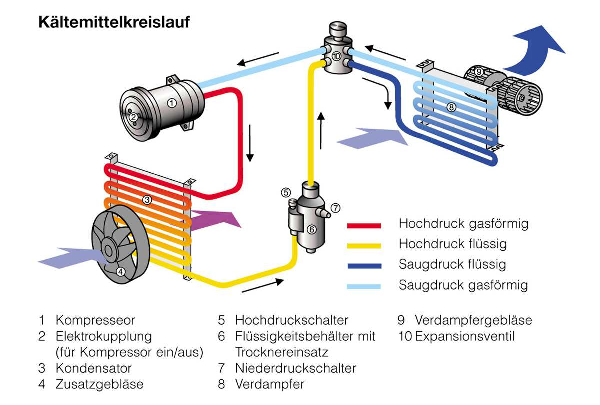
\includegraphics[width=0.7\textwidth]{images/Klima/Klimakreislauf-1.pdf}
\caption{Klimakreislauf}
%\label{fig:}%% anpassen
\end{figure}

\begin{enumerate}
\item
  \textbf{Kompressor} (Gasverdichter, gasförmig, Verdichten, Druck
  steigt) saugt das abgekühlte gasförmige Kältemittel an und verdichtet
  es. Druck und Temperatur steigt (Druckanstieg). Das Kältemittel
  erwärmt sich, wird aber nicht komplett flüssig. Deshalb schieben wir
  es durch den Kondensator.
\item
  \textbf{Kondensator} (Verflüssiger, Kondensieren) hier wird das
  Kältemittel von der Umgebungsluft durchströmt und abgekühlt.
  Aggregatzustand wechsel von gasförmig $\to$ flüssig (Druck ist
  konstant). Kältemittel wird flüssig, wenn es den Kondensator verlässt.
\item
  \textbf{Expansionsventil} (Dosiereinheit, Druckminderer, Drossel,
  Expandieren, flüssig) Kältemittel expandiert durch die Drossel (Druck
  abfall) und lässt bedarfsgerecht eine bestimmte definierte Menge
  Kältemittel durch Strömen.
\item
  \textbf{Verdampfer} (Verdampfen) dadurch wird ein Aggregatzustand
  wechsel von flüssig $\to$ gasförmig (Druck ist konstant)
  gewährleistet. Die durch den Verdampfer strömende Umgebungsluft
  runterkühlen und in den Innenraum einströmen lassen. Dabei entzieht
  das Kältemittel der Umgebungsluft Wärme und kühlt sie ab.
\end{enumerate}

\newpage

\subsection{Kunde bemängelt, Klimaanlage kühlt nicht
richtig}\label{kunde-bemaengelt-klimaanlage-kuehlt-nicht-richtig}

\textbf{Es wurde beispielsweise nur 100 g Kältemittel abgesaugt. Kann
die Klimaanlage wieder befüllt werden?}

Nicht befüllen $\to$ wir machen uns strafbar.

Kältemittel absaugen und mit Stickstoff auf Undichtigkeit prüfen.

\textbf{Verlust an Kältemittel}
$[\%] \, \boxed{= \frac{\text{abgesaugte Menge}}{\text{Füllmenge}} \cdot 100} \quad \text{Beispiel: } \frac{180~g}{640~g} \cdot 100 = 28~\%$

Jährlich ca. $10~\%$ Verlust normal.

\subsection{Was ist der Unterschied zwischen intern und extern geregelte
Klimakompressoren?}\label{was-ist-der-unterschied-zwischen-intern-und-extern-geregelte-klimakompressoren}

\textbf{Intern}, die Stellung der Taumelscheibe und damit die
Fördermenge wird durch ein Regelventil bestimmt. Kann bei Bedarf über
eine Magnetkupplung entkoppelt und damit komplett ausgeschaltet werden.

\emph{Nachteil:} >>kaputt stehen<< eine Klimaanlage nimmt Schaden, wenn
sie nicht regelmäßig eingeschaltet wird (Dichtungen, Schmierung)

\textbf{Extern} keine Magnetkupplung, mit Überlastschutz, Anlage läuft
immer, aber Fördermenge wird runtergeregelt auf ca. $2~\%$

\emph{Nachteil:} Reibung

\subsection{Kältemittel R744 - Problem bei hohen
Außentemperaturen}\label{kaeltemittel-r744-problem-bei-hohen-aussentemperaturen}

Klima funktioniert schlecht bei zu hohen Außentemperaturen
$> 35^\circ\text{C}$. Kältemittel wird nicht genug runtergekühlt.

\subsection{Warum sollte man eine Klimaanlage spülen und welche
Möglichkeiten gibt
es?}\label{warum-sollte-man-eine-klimaanlage-spuelen-und-welche-moeglichkeiten-gibt-es}

Bei Verunreinigungen, Beispiel Kompressor schaden.

\begin{itemize}
\item
  Sieb Einsätze
\item
  Formiergas, Stickstoff, mit Kältemittel (Quelle: Andreas Lamm)
\end{itemize}

\textbf{Offene Anlage} Trockner erneuern oder Anlage verschließen.

\subsection{Desinfizieren einer
Klimaanlage}\label{desinfizieren-einer-klimaanlage}

\begin{itemize}
\item
  Ozongeräte (24h)
\item
  Spray (geringe Wirkung)
\end{itemize}

\subsection{Warum läuft aus der Klimaanlage Wasser bei heißem
Wetter?}\label{warum-laeuft-aus-der-klimaanlage-wasser-bei-heissem-wetter}

\begin{itemize}
\item
  \textbf{Sommer} schwüles Wetter hat eine hohe Luftfeuchtigkeit
\item
  \textbf{Winter} kalte Luft hat eine geringe Luftfeuchtigkeit
\end{itemize}

\subsection{Welche Kältemittelöle gibt es und wo ist der
Unterschied?}\label{welche-kaeltemitteloele-gibt-es-und-wo-ist-der-unterschied}

Herstellerangaben befolgen - Typenschild auf dem Klimakompressor

\begin{itemize}
\item
  \textbf{PAG-Öle} hygroskopisch
\item
  \textbf{POE-Öle} Polyester-Öl, elektrisch isolierendes
  Klimakompressoröl
\end{itemize}

\newpage

\section{Klimaservice}\label{klimaservice}

\textbf{Ruhedruck} (Motor aus)

\begin{itemize}
\item
  Kältemitteldruck abhängig von Umgebungstemperatur (Vgl. Dampftafel /
  Richtwerte \textcite{schmidt:2015:klima} S. 120)
\end{itemize}

\textbf{Betriebsdruck} (Motor an im LL, Klima ON, max. Gebläse, keine
Umluft, Heizung OFF, Temp. LOW, $5 - 10~\text{Min.}$ laufen lassen)

\begin{itemize}
\item
  \textbf{Sollwerte} Quelle: Andreas Lamm \footnote{\url{https://klimacheck.com/}}
\item
  ND $1 - 3~\text{bar}$
\item
  HD $7 - 20~\text{bar}$
\item
  Kühlung

  \begin{itemize}
  \item
    Außentemperatur $20^\circ \text{C} \to 2 - 8^\circ \text{C}$
    \textbf{Ausströmtemperatur}
  \item
    Außentemperatur $30^\circ \text{C} \to \, <15^\circ \text{C}$
    Ausströmtemperatur
  \end{itemize}
\end{itemize}

\subsection{Klimadiagnose}\label{klimadiagnose}

\begin{enumerate}
\item
  Betriebsdruck (Vgl. Sollwerte)

  \begin{itemize}
  \item
    \textbf{Läuft Kondensatorlüfter?}

    \begin{itemize}
    \item
      Wenn Defroster EIN, dann muss Lüfter laufen!
    \end{itemize}
  \end{itemize}
\item
  Ausströmtemperatur (Vgl. Sollwerte)
\item
  Zustand Kältemittel (Schauglas)
\end{enumerate}

\emph{Vgl. Diagnosetabelle}

\begin{table}[!ht]% hier: !ht 
\centering 
	\caption{}% \label{tab:}%% anpassen 
\begin{tabular}{@{}lll@{}}
\hline
\textbf{Hochdruck} & \textbf{Niederdruck} & \textbf{Ursache} \\
\hline
normal, zu hoch & zu niedrig & Expansionsventil, Filter, Kondensator \\
normal, zu niedrig & zu hoch & zu viel Kältemittel, Kompressor \\
normal, zu niedrig & zu niedrig & zu wenig Kältemittel,
Magnetkupplung \\
zu niedrig & zu hoch & zu viel Kältemittel, Kondensator,
Kondensatorlüfter \\
\hline
\end{tabular} 
\end{table}

Anhand der Leitungstemperaturen auf mögliche Defekte im
Kältemittelkreislauf schließen (\textcite{schmidt:2015:klima} S. 115).

Übersicht über fehlerhafte Füllmengen und Komponenten, die sich an den
Druckmanometern widerspiegeln können (\textcite{schmidt:2015:klima} S. 116
-- 117).

\subsection{Magnetkupplung und Kondensatorlüfter
prüfen}\label{magnetkupplung-und-kondensatorluefter-pruefen}

\textbf{Magnetkupplung am Kompressor prüfen}

\begin{enumerate}
\item
  Spannungsversorgung prüfen (Verkabelung, Sicherung, Relais)

  \begin{enumerate}
  \def\labelenumii{\arabic{enumii}.}
  \item
    Magnetkupplung (Spannung am Verbraucher) Soll: $12~V$
  \item
    Masseanschluss (gegen Masse) Soll: $0~V$
  \item
    Relais (gegen Masse) Soll: $12~V$
  \item
    Druckschalter (gegen Masse) Soll: $12~V$
  \end{enumerate}
\item
  Temperatur- und Druckschalter, Steuergerät, Luftspalt
\end{enumerate}

\textbf{Kondensatorlüfter prüfen}

\begin{itemize}
\item
  Sicherung, Relais, Verkabelung, Motor, schwergängig
\end{itemize}

\subsection{Klima-Service-Gerät}\label{klima-service-geraet}

\begin{itemize}
\item
  Vakuumzeit
  $\boxed{60~Min/kg \cdot \text{Kältemittelmenge [kg]}} \quad (1~h~\hat =~ 1~kg)$
\item
  Füllung
\item
  Kompressor-Öl
\end{itemize}

Phasen

\begin{enumerate}
\item
  \textbf{Absaugen} (von Kältemittel und Kompressoröl)
\item
  \textbf{Evakuieren} (Vakuum, Wasser entfernen, Dichtigkeit prüfen)
\item
  \textbf{Aufbereiten} (Kältemittel von Wasser und Öl trennen und
  wiegen)
\item
  \textbf{Auffüllen} (von Kältemittel und Kompressoröl)
\end{enumerate}

\chapter{06-Loesung-Klimaanlage}
%%ju 31-Dez-22 06-Loesung-Klimaanlage.tex
ANTWORT: Vgl. Fotos 06-L-Klimaanlage-1 bis 3 -Limburg.jpg

\textbf{1. Welche Aufgaben hat eine Klimaanlage im Kfz?}

\textbf{2. Wer ist nach der UVV Sachkundiger im Umgang mit
Klimaanlagen?}

\textbf{3. Beschreiben Sie den Kältemittelkreislauf in einer
Kfz-Klimaanlage.}

\textbf{4. Wie werden in Kfz-Klimaanlagen die Druckbereiche unterteilt
und welche Drücke herrschen in den einzelnen Bereichen vor?}

\textbf{5. Auf welche Weise wird der Klima-Kompressor geschmiert?}

\textbf{6. Welche Aufgaben muss der Flüssigkeitsbehälter mit
Trocknereinsatz in einer Kfz- Klimaanlage übernehmen?}

\textbf{7. Welche Schutzausrüstung muss bei Arbeiten an der
Kfz-Klimaanlage getragen werden?}

\textbf{8. An welchen Orten dürfen Kältemittel gelagert werden?}

\textbf{9. Welche Angaben müssen an jeder Klimaanlage deutlich erkennbar
und dauerhaft angebracht sein?}

\textbf{10. Warum muss eine Kfz-Klimaanlage in gewissen Zeitabständen
gewartet werden?}

\chapter{07-Gemischbildung-Diesel-I}
%%ju 26-Dez-22 07-Gemischbildung-Diesel-I.tex
\textbf{1892} erfand >>Rudolf Diesel<< den Motor, der heute PKW, LKW,
Busse, Schiffe, Panzer, Baumaschinen, Landmaschinen und Gabelstapler
antreibt und der auch stationär zur Stromerzeugung eingesetzt wird.

\section{Eigenschaften Dieselmotor}\label{eigenschaften-dieselmotor}

\begin{enumerate}
\item
  Selbstzündung (Kompressionszündung)
\item
  Innere Gemischbildung (Brennraum)
\item
  Qualitative Gemischregulierung (Die eingespritzte Kraftstoffmenge
  reguliert die Leistung des Motors.)
\item
  Heterogenes Gemisch (Das Gemisch aus Luft und Kraftstoff ist im
  Brennraum nicht gleichmäßig verteilt.)
\item
  Hohes Luftverhältnis (Luftüberschuss, d.h. das Verhältnis von Luft zu
  Kraftstoff ist sehr groß.)
\item
  Zündwilliger Kraftstoff (hoch siedend, hohe Cetanzahl)
\end{enumerate}

\section{Warum gibt es einen Klopfsensor beim
Diesel?}\label{warum-gibt-es-einen-klopfsensor-beim-diesel}

Einspritzüberwachung (früher Nadelbewegungssensor): Einspritzbeginn,
Zündbeginn, wie sauber ist die Verbrennung?

\textbf{Was ist ein Klopfsensor?} (am Motorblock verbaut) Piezo-Element:
wenn die seismische Masse in Schwingung gerät, wird durch die Bewegung
eine Spannung erzeugt und im SG verarbeitet. Eine klopfende Verbrennung
wird durch eine ungewöhnlich große Schwingung im Motor erkannt.

\section{Welche Arten von Dieselmotoren gibt
es?}\label{welche-arten-von-dieselmotoren-gibt-es}

\begin{itemize}
\item
  Direkteinspritzung (erste 1988 Audi)
\item
  Indirekte Einspritzung (Vorkammer und Wirbelkammer)

  \begin{itemize}
  \item
    kugelförmig - Vergrößerung der Oberfläche - Wärmeverluste $\to$
    kompensieren durch hohe Drücke und Temperaturen
  \item
    Vorverbrennung $\to$ weiche Verbrennung
  \end{itemize}
\item
  Saugrohreinspritzung
\item
  Turbo aufgeladen
\end{itemize}

\section{Warum haben wir eine höhere Verdichtungsendtemperatur als die
Selbstentzündungstemperatur?}\label{warum-haben-wir-eine-hoehere-verdichtungsendtemperatur-als-die-selbstentzuendungstemperatur}

Das Gemisch muss sich schlagartig und schnell genug entzünden und sauber
genug durchbrennen.

Gay-Lussac - Faktor 2 S. 193 (\textcite{brand:2020:fachkundeKfz}) Erwärmt
man das Gas um $273~K$, so dehnt es sich auf das doppelte aus.
Verhindert man die Ausdehnung beim Verdichten, so verdoppelt sich der
Druck.

\begin{itemize}
\item
  Verdichtungsverhältnis: $14 - 27:1$
\item
  Verdichtungsendtemperatur (Lufttemperatur):
  $600 - 900^\circ\text{C}$
\item
  Verdichtungsenddruck: $30 - 55~\text{bar}$
\item
  Selbstzündungstemperatur (untere Grenze) $220^\circ\text{C}$ (im
  Mittel) bei ca. $350^\circ\text{C}$ Quelle: Bosch S. 562
  (\textcite{reif:2022:boschkraftfahrtechnisches}).
\item
  Verbrennungshöchstdruck: $200~\text{bar}$
\item
  Druck beim Öffnen des Auslassventils: $4 - 6~\text{bar}$
\item
  Abgastemperatur: $550 - 750^\circ\text{C}$
\end{itemize}

\textbf{vgl. Otto-Saugmotor}

\begin{itemize}
\item
  Verdichtungsverhältnis: $7-12:1$
\item
  Verdichtungsendtemperatur (Lufttemperatur) $400 - 500^\circ\text{C}$
\item
  Verdichtungsenddruck: $18~\text{bar}$
\item
  Selbstzündungstemperatur (im Mittel) $500^\circ\text{C}$ Quelle:
  Bosch S. 562 (\textcite{}reif:2022:boschkraftfahrtechnische)
\item
  Verbrennungshöchstdruck: $30 - 60~\text{bar}$
\item
  Druck beim Öffnen des Auslassventils: $3 - 5~\text{bar}$
\item
  Abgastemperatur: $900^\circ\text{C}$
\end{itemize}

Ein \textbf{Arbeitsspiel} läuft in zwei Kurbelwellenumdrehungen ab
$720^\circ\text{KW}$ (Kurbelwinkel). Die \textbf{vier Takte des
Arbeitsspieles} sind Ansaugen, Verdichten, Arbeiten und Ausstoßen.
\textbf{Ein Takt} ist zwischen UT und OT.

\textbf{Ottomotor / Saugrohreinspritzung}

\begin{enumerate}
\item
  Motor / Drosselklappe (fast geschlossen -- offen)
\item
  Ansaugen (geringe -- maximale Menge Kraftstoff-Luftgemisch)
\item
  Füllung (schlecht -- maximal)
\item
  Verdichtungshöchstdruck (gering -- maximal)
\item
  Zündung des Kraftstoff-Luftgemisches, nach der Verbrennung
\item
  Verbrennungshöchstdruck (gering -- maximal)
\item
  wirkt auf die Kolbenfläche und wird auf $\to$ Kolben $\to$ Pleuel
  $\to$ Kurbelwelle übertragen
\item
  Drehmoment an Kurbelwelle (gering -- maximal)
\item
  Drehzahl des Motors (gering -- maximal)
\end{enumerate}

\section{Nageln}\label{nageln}

\textbf{Nageln} ist ein harter Motorlauf und entsteht durch zu großer
Zündverzug, zum Beispiel beim Kaltstart des Motors (schlagartige
Verbrennung), kann gemindert werden durch Voreinspritzung.

\textbf{Zu großer Zündverzug tritt ein \ldots{}}

\begin{enumerate}
\item
  kaltem Motor oder kalter Ansaugluft
\item
  schlechter Kompression
\item
  Kraftstoff mit zu niedriger Cetanzahl
\item
  tropfenden Injektoren
\end{enumerate}

\section{Quantitätsregelung und
Qualitätsregelung}\label{quantitaetsregelung-und-qualitaetsregelung}

\textbf{Quantitätsregelung} Ottomotor - Regulierung über die
Gemischmasse, Drosselklappe (Lastzustand) Menge von Luftmasse
(Luftmassenmesser) und Kraftstoffmasse, um das Ziel Lambda = 1 zu
erreichen, wird die Kraftstoffmasse angepasst.

\textbf{Qualitätsregelung} Dieselmotoren - Regulierung über die
Kraftstoffmasse, keine Drosselklappe (systembedingt) nahezu konstante
gleiche Menge Luftmasse, aber die Größe der Kraftstoffmasse kann
geändert werden in Abhängigkeit des Lastwunsches.

\section{Verbrennungsablauf beim
Dieselmotor}\label{verbrennungsablauf-beim-dieselmotor}

\textbf{Verbrennung am Kraftstofftröpfchen} Ausgangslage: Dieseltropfen
wird eingespritzt, Umgebungsluft $600 - 900^\circ\text{C}$,
Kraftstofftröpfchen so gut wie möglich zu verdampfen.

Das Ziel ist ein zündfähiges Gemisch an der Außenlufttemperatur von
selbst zu entzünden, da nur eine sehr geringe Zeit zwischen
Einspritzzeit und kurz vor Ende des Verbrennungsprozesses besteht. Um
die Kraftstofftröpfchen so klein wie möglich zu halten, werden sehr hohe
Drücke und Temperaturen angestrebt.

\textbf{Unvollständige Verbrennung} (durch Sauerstoffmangel)

Wie kann das sein, wir haben doch Sauerstoffüberschuss?

Je größer der Kraftstofftropfen, desto größer ist der Bereich, wo
Luftmangel herrscht.

\textbf{Ursachen für Partikel und Rußbildung} durch unvollständige
Verbrennung

\begin{enumerate}
\item
  Kaltstart- und Warmlaufphase (kalter Motor hat geringere Kompression,
  Kondensationsverluste an Zylinderwand, Wärmeabgabe an Brennraumwände)
\item
  Volllastbetrieb (Kraftstoffüberschuss)
\item
  Sauerstoffmangel (verstopfter Luftfilter, defekter Turbolader,
  undichter Ladeluftkühler)
\item
  Defekte Injektoren (schlechtes Strahlbild, tropfen nach $\to$ mehr
  Kraftstoff)
\item
  Kompressionsverluste (Blow-by, Verdichtungstemperatur wird später
  erreicht)
\end{enumerate}

\section{Was ist EDC? Nenne Aufgaben, Vorteile, Ziele und
Merkmale}\label{was-ist-edc-nenne-aufgaben-vorteile-ziele-und-merkmale}

\textbf{EDC} (Electronic Diesel Control, elektronische Dieselsteuerung,
Motorsteuerung), Kennfeld (Sollwerte) geregeltes elektronisches
Einspritzsystem (Einspritzsteuerung)

\textbf{Motorsteuerung Aufgaben} (Auswahl)

\begin{enumerate}
\item
  Einspritzung des Kraftstoffes

  \begin{itemize}
  \item
    zu jedem Zeitpunkt die gerade erforderliche Menge an Kraftstoff in
    die Zylinder des Motors einzuspritzen.
  \end{itemize}
\item
  Regelung und Begrenzung von Drehzahl und Geschwindigkeit,
\item
  Regelung des Luftsystems (Abgasrückführung und Ladedruckregelung),
\item
  Abgasnachbehandlung,
\item
  Glühkerzensteuerung und Thermomanagement,
\item
  Zylinderabschaltung,
\item
  Diagnose,
\item
  Wegfahrsperre.
\end{enumerate}

\textbf{Vorteile} bedarfsgerechte Regelung

\textbf{Ziele} Einspritzbeginn und Kraftstoffmenge exakt zu regeln

\textbf{Merkmale} Optimieren von Schadstoffen, Verbrauch, Drehmoment und
Leistung, Laufruhe

\section{Was sind die Hauptsteuergrößen eines jeden
Motors?}\label{was-sind-die-hauptsteuergroessen-eines-jeden-motors}

Last und Drehzahl (Fahrpedalwertsensor, Drehzahlsensor der Kurbelwelle)

\textbf{Korrektursteuergrößen} anpassen der Grundeinspritzzeiten
(abhängig vom Motor)

Einspritzbeginn, $NO_\text{x}-\text{Wert}$, Motortemperatur,
Fahrgeschwindigkeit, AGR-Rate, Ladedruck, Ansauglufttemperatur,
Kraftstofftemperatur, usw.

\section{Einspritzsysteme}\label{einspritzsysteme}

\begin{enumerate}
\item
  \textbf{Reiheneinspritzpumpe}

  \begin{itemize}
  \item
    Einspritzdruck bis etwa 1300 bar
  \item
    Mengenregelung und Förderbeginn (Fliehkraftregler)
  \end{itemize}
\item
  \textbf{Axialkolben-Verteilereinspritzpumpe} (VE)

  \begin{itemize}
  \item
    Einspritzdruck bis etwa 1400 bar
  \item
    Mengenregelung (Verschieben des Regelschiebers) und Förderbeginn
    (hydraulische Spritzversteller), Drehzahl (Fliehkraftregler)
  \end{itemize}
\item
  \textbf{Radialkolben-Verteilereinspritzpumpe} (VP44)

  \begin{itemize}
  \item
    Einspritzdruck bis etwa 1900 bar
  \end{itemize}
\item
  \textbf{Pumpe-Düse System mit Magnetventil}

  \begin{itemize}
  \item
    Einspritzdruck bis etwa 2200 bar
  \end{itemize}
\item
  \textbf{Pumpe-Düse System mit Piezoventil}
\item
  \textbf{Pumpe-Leitung-Düse System} (PLD, Nfz)
\item
  \textbf{Common-Rail System}
\end{enumerate}

\subsection{Pumpe-Leitung-Düse
System}\label{pumpe-leitung-duese-system}

Pro Zylinder ein Pumpenelement und eine Einspritzdüse. Einspritzdruck
bis etwa 1800 bar. Eine elektrisch geregelte Voreinspritzung ist
aufgrund der Trägheit des Systems nicht möglich (Länge der
Kraftstoffwege). Um eine Voreinspritzung realisieren zu können, kommen
spezielle Einspritzdüsen zum Einsatz. Die sogenannten
Zweifeder-Düsenhalter (kleine Feder - Voreinspritzung, große Feder -
Haupteinspritzung).

\newpage

\subsection{Pumpe-Düse System mit
Magnetventil}\label{pumpe-duese-system-mit-magnetventil}

\textbf{Erkläre die Vorgänge - Befüllen, Voreinspritzung,
Haupteinspritzung eines PDE}

\textbf{Befüllen} bei ablaufenden Einspritznocken wird der Pumpenkolben
nach oben gezogen und der Hochdruckraum wird mit Kraftstoff befüllt.
Solange Magnetventil offen ist, fließt der Kraftstoff durch den
Hochdruckraum in den Rücklauf ab. (kühlende Wirkung)

Bei auflaufenden Nocken wird der Pumpenkolben nach unten gedrückt. Das
\emph{Magnetventil} ist geschlossen und verschließt Kraftstoff Vor- und
Rücklaufleitung. Es baut sich ein Hochdruck auf.

\textbf{Voreinspritzung} (Beginn) bei etwa 180 bar ist der Druck größer
als die Düsen-Federkraft. Durch das Einspritzen des Kraftstoffs haben
wir einen kurzen Druckabfall und die Düsennadel schließt (Ende).

Der Ausweichkolben hat seine schräge Druckschulter freigegeben (große
Fläche, große Kraft), wodurch er nach unten gedrückt wird und spannt die
Düsenfeder vor.

\emph{Magnetventil} öffnet und der überschüssige Kraftstoff entweicht in
die Vor- und Rücklaufleitung.

\textbf{Haupteinspritzung} der Druck steigt weiter und drückt bei etwa
300 bar die Düsennadel nach oben (Ende). Durch den Druckabfall schließt
die Düsennadel.

\textbf{Nachteile des Pumpe-Düse Systems mit Magnetventil}

\begin{enumerate}
\item
  Druckerzeugung ist abhängig von Einspritznocken zum Pumpenkolben
\item
  Druck ist nicht konstant, sondern 300 bis 2200 bar
  (Kraftstofftröpfchengröße)
\item
  Hohe Kräfte können auf den Zahnriemen wirken
\item
  Keine Nacheinspritzung (zu Regeneration von DPF)
\item
  Kein mehrmaliges Vorspritzen möglich
\end{enumerate}

\newpage

\begin{figure}[!ht]% hier: !ht
\centering
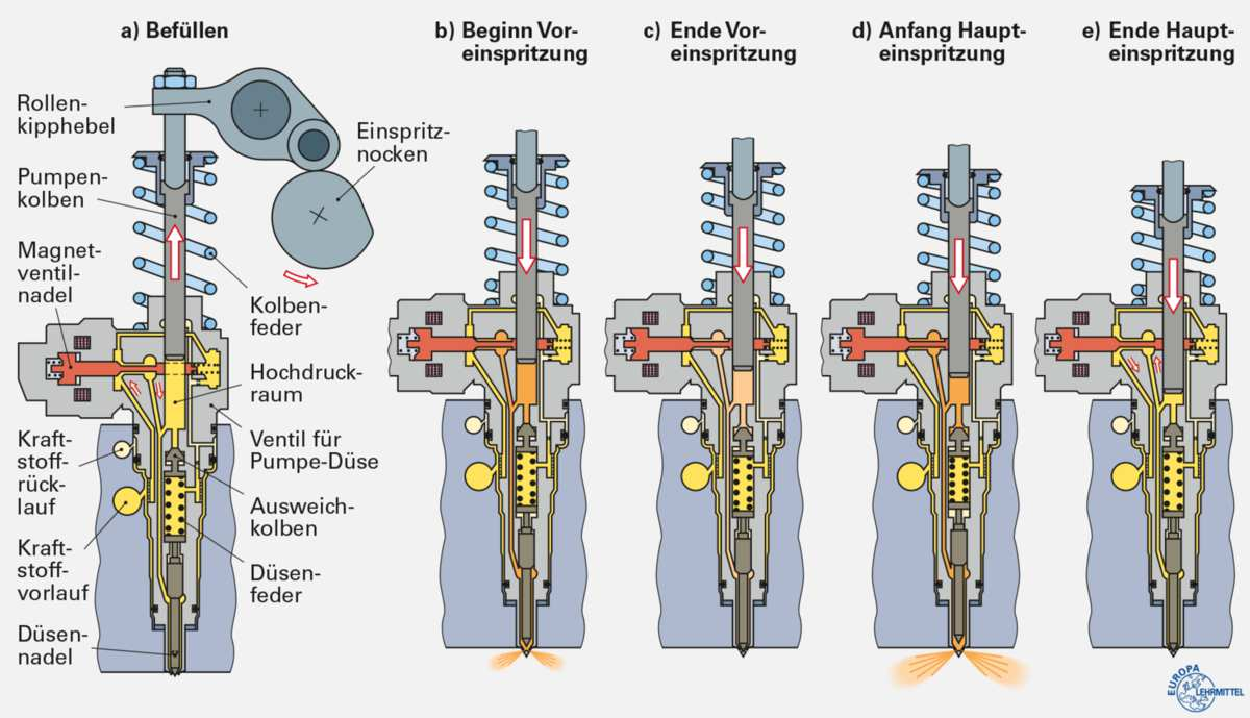
\includegraphics[width=0.7\textwidth]{images/Diesel/Diesel-11.pdf}
\caption{Pumpe-Düse System, Quelle: Europa-Verlag}
%\label{fig:}%% anpassen
\end{figure}

\begin{enumerate}
\item
  Drallkanal
\item
  Füllkanal
\item
  Auslasskanal
\item
  Einlassnockenwelle
\item
  Kraftstoffrücklauf
\item
  Auslassnockenwelle mit Einspritznocken
\item
  Kolbenfeder
\item
  Einspritznocke
\item
  Rollenkipphebel
\item
  Ausweichkolben
\item
  Pumpenkolben
\item
  Magnetventil PDE
\item
  Einstellschraube Spielausgleich PDE
\item
  Kraftstoffzulauf
\item
  Hochdruckraum
\end{enumerate}

\textbf{Einspritzvorgang}

\begin{enumerate}
\item
  Nockenhub wird über den Rollenkippebel auf den Pumpenkolben übertragen
\item
  \textbf{Magnetventil angesteuert} und verschließt Kraftstoffzulauf und
  -rücklauf
\item
  Druckaufbau im Hochdruckraum beginnt
\item
  Bei ca. 180 bar ist der Druck größer als die Federkraft.
  \textbf{Voreinspritzung beginn}
\item
  Ausweichkolben öffnet Ausgleichsraum, kurzer Druckabfall.
  \textbf{Voreinspritzung ende}
\item
  Bei ca. 300 bar überwindet der Kraftstoffdruck die Kraft der
  vorgespannten Feder. \textbf{Haupteinspritzung beginn}
\item
  \textbf{Magnetventil nicht angesteuert} und öffnet den
  Kraftstoffzulauf und -rücklauf.
\end{enumerate}

\textbf{steile Flanke des Einspritznockens} bewirkt einen schnellen
Druckanstieg.

\subsection{Pumpe-Düse System mit
Piezoventil}\label{pumpe-duese-system-mit-piezoventil}

\textbf{Piezoelektrische-Effekt} (direkt), übt man auf einen
Piezokristall Druck aus, so erzeugt dieser eine Spannung.

\emph{Verformung} durch Druck / Krafteinfluss

\emph{Anwendung:} Klopfsensor, Drucksensor (Click-Feuerzeug)

\textbf{Reziproker Piezoelektrischer-Effekt} (invers) legt man an einen
Piezokristall eine Spannung an, so verformt er sich. Die Längenänderung
ist proportional zur angelegten Spannung.

\emph{Verformung} durch Spannungseinfluss

\emph{Anwendung:} Injektor

Kfz: Steuerspannung 110-150 V, max. Ausdehnung 0,15 \%

Piezoventil ersetzt Magnetventil (Trägheit - Magnetventil bewegt sich
zeitversetzt, weil der Magnetfeldaufbau gehemmt wird, durch
Gegeninduktion)

\textbf{Piezoventil (Piezoaktor)} besteht aus Piezoaktormodul und
Übersetzermodul (kl. Hebelwerk)

Die Längenausdehnung eines Piezokristalls liegt bei maximal 0,15 \%
(sehr gering). Werden, bis zu 500 Piezokristalle in Reihe geschaltet ist
die Gesamtausdehnung des Piezoaktormodul etwa 0,04 mm. Zum Erreichen der
erforderlichen Ventilöffnung von 0,1 mm wird ein kleines Hebelwerk,
sogenannte Übersetzermodul zwischen Piezoaktormodul und hydraulischen
Ventil geschaltet.

\textbf{Piezoventil geschlossen}, die Verbindung zwischen Hochdruckraum
zur Vor- und Rücklaufleitung ist unterbrochen. Hochdruck kann sich
aufbauen und es wird eingespritzt.

\textbf{Piezoventil offen}, die Verbindung zwischen Hochdruckraum zur
Vor- und Rücklaufleitung ist wieder hergestellt. Hochdruck entweicht und
der Einspritzvorgang ist beendet.

\section{Einspritzventile}\label{einspritzventile}

\begin{itemize}
\item
  Ein- und Zweifeder-Düsenhalter
\item
  Loch- und Zapfendüsen
\end{itemize}

\textbf{Prüfen:} Öffnungsdruck, Strahlbild

\section{Glühsysteme}\label{gluehsysteme}

\textbf{Aufgabe von Starthilfsanlagen}

\begin{enumerate}
\item
  Anspringen des kalten Dieselmotors erleichtern
\item
  runden und stabilen Leerlauf zu sorgen
\item
  Schadstoffemissionen zu senken
\end{enumerate}

\textbf{Arten von Glühstiftkerzen}

\begin{enumerate}
\item
  \textbf{Selbstregelnde Glühstiftkerzen}

  \begin{itemize}
  \item
    \emph{Aufbau:} Heizwendel, Regelwendel, Keramikstift, Ringspalt
  \item
    \emph{Nennspannung:} 11,5 V
  \item
    \emph{Vorglühzeit:} 2 -- 7 s
  \item
    \emph{Glühtemperatur:} $850^\circ\text{C}$
  \item
    \emph{Leistungsaufnahme:} 100 W
  \item
    \emph{Regelung der Glühkerzenstromaufnahme:} Durch das PTC-Verhalten
    der Regelwendel wird die Stromaufnahme nach erreichen der
    Glühtemperatur begrenzt.
  \end{itemize}
\item
  \textbf{Elektronisch geregelte Glühstiftkerzen}

  \begin{itemize}
  \item
    \emph{Aufbau:} Heizwendel, Regelwendel, Keramikstift, Ringspalt
  \item
    \emph{Nennspannung:} 5 -- 8 V
  \item
    \emph{Vorglühzeit:} 1 -- 2 s
  \item
    \emph{Glühtemperatur:} $1000^\circ\text{C}$
  \item
    \emph{Regelung der Glühkerzenstromaufnahme:} Die Glühkerzen werden
    pulsweitenmoduliert kurzfristig mit Überspannung von bis zu 11 V
    betrieben.
  \end{itemize}
\item
  \textbf{Drucksensorglühstiftkerzen} (PSG, Pressure Sensor Glow Plug,
  Brennraumdruckgeber)

  \begin{itemize}
  \item
    Einspritzzeitpunkt und Druckverlauf ermitteln
  \end{itemize}
\end{enumerate}

\chapter{07-Loesung-Gemischbildung-Diesel-I}
%%ju 31-Dez-22 07-Loesung-Gemischbildung-Diesel-I.tex
\textbf{1) Was versteht man unter innerer Gemischbildung beim
Dieselmotor?}

Darunter versteht man, dass das Gemisch im Zylinderraum des Motors
entsteht. Der Dieselkraftstoff also erst dort mit der Ansaugluft in
Berührung kommt.

\textbf{2) Definieren Sie Quantitätsregelung und Qualitätsregelung.}

\begin{enumerate}
\item
  Unter einer \textbf{Quantitätsregelung} versteht man, dass der Motor
  durch eine Anpassung der Gemischmasse zum Beispiel durch eine
  Drosselklappe geregelt wird.
\item
  Bei einer \textbf{Qualitätsregelung} erfolgt die Luftzufuhr nahezu
  Last unabhängig. Lediglich die Kraftstoffmasse wird mit zunehmender
  Last erhöht.
\end{enumerate}

\textbf{3) Bei welcher Temperatur wird Dieselkraftstoff zündfähig und
wann entzündet er sich von selbst?}

\begin{enumerate}
\item
  zündfähig bei etwa $60^\circ\text{C}$
\item
  Selbstzündungstemperatur (untere Grenze) $220^\circ\text{C}$ (im
  Mittel) bei ca. $350^\circ\text{C}$ Quelle: Bosch S. 562
  (\textcite{reif:2022:boschkraftfahrtechnisches}).
\end{enumerate}

\textbf{4) Erklären Sie ausführlich den Verbrennungsablauf im Brennraum
eines direkt einspritzenden Dieselmotors.}

Gegen Ende des Verdichtungstaktes wird Dieselkraftstoff fein zerstäubt,
in die $600 - 900^\circ\text{C}$ heiße Luft eingespritzt. Diese
verdampft über die Oberfläche der entstandenen Kraftstofftropfen. Je
feiner die Zerstäubung des Kraftstoffes, desto größer ist die Oberfläche
im Verhältnis zum Volumen, was den Vergasungsprozess begünstigt. Die
gasförmigen Kohlenwasserstoffe vermischen sich mit der Ansaugluft und
erhitzen sich, bis sich bei ca. $220^\circ\text{C}$ zur
Selbstentzündung des Kraftstoffes kommt. Je nach System wird dieser
Vorgang Last- und Drehzahlabhängig in mehreren Vorgängen unterteilt, um
den Druckanstieg im Zylinder und damit die Laufkultur des Motors zu
begünstigen.

\textbf{5) Unter welchen motorischen Bedingungen entstehen beim
Dieselmotor unverbrannte Kohlenwasserstoffe?}

\begin{enumerate}
\item
  Kaltstart- und Warmlaufphase (kalter Motor hat geringere Kompression,
  Kondensationsverluste an Zylinderwand, Wärmeabgabe an Brennraumwände)
\item
  Volllastbetrieb (Kraftstoffüberschuss)
\item
  Luftmangel (verstopfter Luftfilter, defekter Turbolader, undichter
  Ladeluftkühler)
\item
  Defekte Injektoren (schlechtes Strahlbild, tropfen nach $\to$ mehr
  Kraftstoff)
\item
  Kompressionsverluste (Verdichtungstemperatur wird später erreicht)
\end{enumerate}

\textbf{6) Warum wird beim Dieselmotor bei Volllast über einen größeren
Zeitraum eingespritzt?}

Da bei Volllast der maximale Einspritzdruck eingestellt wird, geht die
Mengenregelung nur über die Zeit.

\textbf{7) Wie groß ist beim Dieselmotor der Luftüberschuss bei Leerlauf
/ Volllast?}

\begin{itemize}
\item
  Leerlauf $\lambda = 10 \dots 18$
\item
  Volllast $\lambda = 1,15 \dots 2$
\end{itemize}

(Luftzahl / Lambda)

\textbf{8) Definieren Sie Zündverzug. Wie groß ist der Zündverzug?}

Die Zeitspanne von Einspritzbeginn an der Einspritzdüse und dem
Zündbeginn des Kraftstoff-Luft-Gemisches im Brennraum.

Zündverzug bei betriebswarmer Motor: 1 ms

\textbf{9) Wodurch kann es bei betriebswarmem Motor zum Nageln kommen?}

Durch einen zu großen Zündverzug.

\textbf{Mögliche Ursachen:}

\begin{enumerate}
\item
  zu früher Einspritzbeginn
\item
  Mangelhafte Kompression
\item
  Luftmangel (verstopfter Luftfilter, defekter Turbolader, undichter
  Ladeluftkühler)
\item
  schlechte Kraftstoffqualität (Cetanzahl zu niedrig)
\item
  Nach tropfende Einspritzdüse
\end{enumerate}

\textbf{10) Warum muss beim indirekt einspritzenden Dieselmotor das
Verdichtungsverhältnis 18 - 24:1 betragen, während beim direkt
einspritzenden Dieselmotor ein Verdichtungsverhältnis von 14 bis 18:1
ausreicht?}

Die Oberfläche des Zylinderraumes ist bedingt durch die Vor- oder
Wirbelkammeroberfläche bei indirekt einspritzenden Dieselmotor größer,
wodurch es zu stärkeren Wärmeverlusten kommt. Diese müssen durch eine
stärkere Erwärmung der Luft, also durch ein höheres
Verdichtungsverhältnis, kompensiert werden.

(Eine höhere Kompression kostet aber auch mehr Kompressionsarbeit.)

\chapter{08-Hybrid}
%%ju 31-Dez-22 08-Hybrid.tex
\textbf{Was ist ein Hybridfahrzeug? Hybrid-Vehicle (HV)} ist mit
mindestens zwei unterschiedlichen Energiewandlern und -speichern für den
Antrieb des Fahrzeuges ausgestattet.

Beispiel: Verbrennungsmotor und Kraftstofftank \& E-Motor und
HV-Batterie

\section{Arten von Hybriden}\label{arten-von-hybriden}

\begin{enumerate}
\item
  \textbf{Micro-Hybrid:} Regeneratives Bremsen, Start-Stopp
\item
  \textbf{Mild-Hybrid:} Regeneratives Bremsen, Start-Stopp,
  Drehmomentunterstützung
\item
  \textbf{Full-Hybrid:} Regeneratives Bremsen, Start-Stopp,
  Drehmomentunterstützung, Elektrisches Fahren
\item
  \textbf{Plug-in-Hybrid:} Regeneratives Bremsen, Start-Stopp,
  Drehmomentunterstützung, Elektrisches Fahren, Steckdosenaufladung
\end{enumerate}

\textbf{Boosten} Drehmomentunterstützung (Verbrennungsmotor
unterstützen)

\textbf{Rekuperation} Regeneratives Bremsen (Bremsenergierückgewinnung
$\to$ Batterie Laden)

\section{Antriebskonzepte}\label{antriebskonzepte}

Leistungsverzweigter Hybrid S. 52 (\textcite{schmidt:2021:hybrid}) und
Antriebskonzepte S. 1000 (\textcite{reif:2022:boschkraftfahrtechnisches}).

E-Maschine = \textbf{MG1 / MG2} (E-Motor / Generator), \textbf{V-Motor}
(Verbrennungsmotor), \textbf{Planetengetriebe} (Planetenradsätze und
Lamellenkupplung), Getriebe, Achsantrieb, Inverter (Pulswechselrichter)

\begin{enumerate}
\item
  \textbf{Serieller Hybrid}

  \begin{itemize}
  \item
    Antrieb: durch E-Motor
  \item
    Verbrennungsmotor wird im Drehzahlfenster betrieben (mechanisch
    nicht mit Antriebstrang verbunden)
  \item
    Serieller Energiefluss

    \begin{enumerate}
    \def\labelenumii{\arabic{enumii}.}
    \item
      V-Motor $\to$ Generator $\to$ Inverter $\leftrightarrow$
      HV-Batterie
    \item
      Inverter $\leftrightarrow$ E-Motor $\leftrightarrow$
      Achsantrieb
    \end{enumerate}
  \item
    Nachteil: schlechter Wirkungsgrad ($3\text{x}$ mehr Leistung
    reinstecken!)
  \item
    Beispiel: Range-Extender (Reichweitenverlängerung)
  \end{itemize}
\item
  \textbf{Paralleler Hybrid}

  \begin{itemize}
  \item
    Antrieb: durch E-Motor oder V-Motor (mechanisch mit Antriebstrang
    verbunden) oder beide parallel
  \item
    \emph{eine Kupplung zwischen E-Maschine $\parallel$ Getriebe -
    Achsantrieb}
  \item
    Energiefluss:

    \begin{enumerate}
    \def\labelenumii{\arabic{enumii}.}
    \item
      V-Motor $\to$ Achsantrieb
    \item
      Batterie $\leftrightarrow$ Inverter $\leftrightarrow$ MG
      $\leftrightarrow$ Achsantrieb
    \end{enumerate}
  \item
    \emph{zwei Kupplungen zwischen V-Motor $\parallel$ E-Maschine
    $\parallel$ Getriebe - Achsantrieb}
  \item
    Energiefluss:

    \begin{enumerate}
    \def\labelenumii{\arabic{enumii}.}
    \item
      V-Motor $\to$ Achsantrieb
    \item
      Batterie $\leftrightarrow$ Inverter $\leftrightarrow$ MG
      $\leftrightarrow$ Achsantrieb
    \end{enumerate}
  \end{itemize}
\item
  \textbf{Leistungsverzweigter Hybrid}

  \begin{itemize}
  \item
    Antrieb: durch zwei E-Motoren und V-Motor (mechanisch mit
    Antriebstrang verbunden)
  \item
    Nachteil: aufwändiges Getriebe
  \item
    Leistungsverzweigung (Planetengetriebe)
  \item
    V-Motor (Drehmoment aufteilen)

    \begin{enumerate}
    \def\labelenumii{\arabic{enumii}.}
    \item
      Teil $\to$ MG1 als Generator
    \item
      Teil $\to$ Fahrzeugantrieb
    \end{enumerate}
  \item
    V-Motor + E-Motor $\to$ Fahrzeugantrieb
  \item
    Schub- u. Bremsphase: Generator $\to$ Rekuperation
  \end{itemize}
\end{enumerate}

\chapter{09-Common-Rail-Diesel-II}
%%ju 26-Dez-22 09-Common-Rail-Diesel-II.tex
\section{Bauteile und Aufgaben eines Common-Rail
Systems}\label{bauteile-und-aufgaben-eines-common-rail-systems}

\begin{figure}[!ht]% hier: !ht
\centering
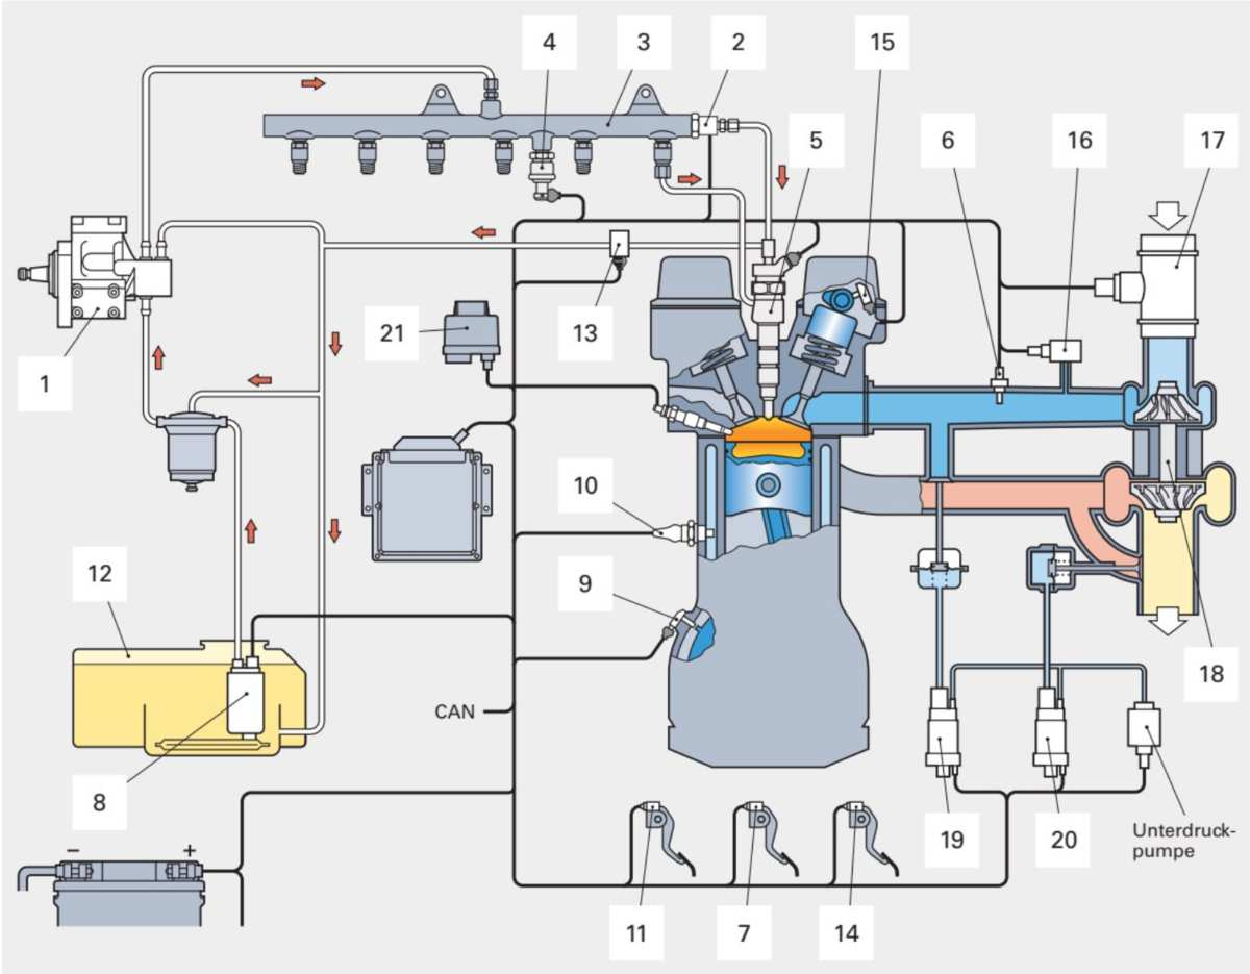
\includegraphics[width=0.7\textwidth]{images/Diesel/Diesel-6.pdf}
\caption{Common-Rail System, Quelle: Europa-Verlag}
%\label{fig:}%% anpassen
\end{figure}

\begin{enumerate}
\item
  \textbf{Hochdruckpumpe} Kraftstoff unter Hochdruck in das Rail
  fördern.
\item
  \textbf{Raildruckregelventil} den erforderlichen Hochdruck an jeden
  Betriebszustand anpassen.
\item
  \textbf{Rail} Hochdruck speichern und Verteilung des Kraftstoffs auf
  die Injektoren.
\item
  \textbf{Raildrucksensor} Hochdruck erfassen und als elektrisches
  Signal an das Steuergerät weiterleiten.
\item
  \textbf{Injektor} Kraftstoff dosiert in den Brennraum spritzen
\item
  Saugrohrtemperaturfühler
\item
  Bremspedalschalter
\item
  \textbf{Vorförderpumpe,} Kraftstoff zu Hochdruckpumpe fördern.
\end{enumerate}

\textbf{Laufruheregelung}, die einzelnen Zylinder bekommen mehr oder
weniger Kraftstoff vom Steuergerät zugeteilt.

\section{Welche Ursachen kommen für den Leistungsverlust
infrage?}\label{welche-ursachen-kommen-fuer-den-leistungsverlust-infrage}

\begin{enumerate}
\item
  \textbf{Mechanische Fehler}

  \begin{itemize}
  \item
    Kompressionsverlust durch Verschleiß der Ventile oder Kolben
  \item
    Verschleiß der Hochdruckpumpe
  \end{itemize}
\item
  \textbf{Fehler im hydraulischen System}

  \begin{itemize}
  \item
    Undichtigkeit an Injektoren (schließt nicht korrekt, tropft nach,
    Düse ausgewaschen)
  \item
    Undichte Leitungen am Rail
  \end{itemize}
\item
  \textbf{Elektrische Fehler}

  \begin{itemize}
  \item
    Sensoren defekt
  \item
    Aktoren defekt
  \item
    Leitungsunterbrechung
  \item
    Masseschluss
  \end{itemize}
\end{enumerate}

\section{Was muss beachtet werden beim Einbau eines neuen
Injektors?}\label{was-muss-beachtet-werden-beim-einbau-eines-neuen-injektors}

\begin{itemize}
\item
  Fertigungstoleranz: muss im Steuergerät einprogrammiert werden
\item
  Zahlen- und Buchstabencodes auf dem Injektor
\item
  Steuergerät korrigiert entsprechend die Grundeinspritzmenge des
  jeweiligen Injektors.
\end{itemize}

\newpage

\section{Welche Druckregelungsarten gibt es?
(Prüfung)}\label{welche-druckregelungsarten-gibt-es-pruefung}

\begin{figure}[!ht]% hier: !ht
\centering
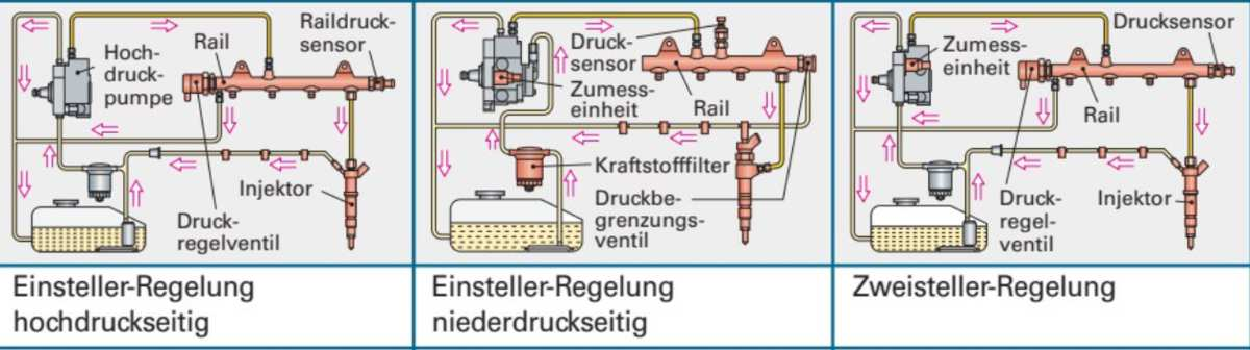
\includegraphics[width=0.8\textwidth]{images/Diesel/Diesel-2.pdf}
\caption{CR-Einsteller- und Zweistellerregelung, Quelle: Europa-Verlag}
%\label{fig:}%% anpassen
\end{figure}

\begin{enumerate}
\item
  \textbf{Einsteller-Regelung}

  \begin{itemize}
  \item
    \textbf{Druckregelung hochdruckseitig} über ein
    \textbf{Druckregelventil} (DRV)

    \begin{itemize}
    \item
      Hochdruckpumpe fördert die maximale Fördermenge unabhängig von
      Bedarf an Kraftstoff
    \item
      Raildruck wird über ein \textbf{Druckregelventil} geregelt, nicht
      benötigter Kraftstoff fließt zurück in den Tank
    \item
      \textbf{Vorteil}

      \begin{itemize}
      \item
        schneller Druckaufbau möglich
      \item
        bei Lastwechsel agil
      \end{itemize}
    \item
      \textbf{Nachteil:} Hochdruckpumpe ist konstant maximal belastet,
      dadurch

      \begin{itemize}
      \item
        geringere Nutzleistung
      \item
        erhöhter Kraftstoffverbrauch, Schadstoffausstoß, Verschleiß
      \item
        unnötige Erwärmung des Kraftstoffs
      \end{itemize}
    \end{itemize}
  \item
    \textbf{Druckregelung niederdruckseitig} (Mengenregelung) über eine
    \textbf{Zumesseinheit} (ZME)

    \begin{itemize}
    \item
      \textbf{Zumesseinheit} regelt die Zuflussmenge zur Hochdruckpumpe
    \item
      \textbf{Bedarfsregelung}, d.h. es gelangt nur so viel Kraftstoff
      zu Hochdruckpumpe wie für die Einspritzung benötigt wird
    \item
      \textbf{Druckbegrenzungsventil} verhindert zu hohen Raildruck bei
      Ausfall der Zumesseinheit
    \item
      \textbf{Vorteil}

      \begin{itemize}
      \item
        bedarfsgerechte Förderung
      \item
        geringe Leistungsaufnahme der Pumpe
      \end{itemize}
    \item
      \textbf{Nachteil:}

      \begin{itemize}
      \item
        hohe Trägheit
      \item
        Drucksteigerung erfordert zunächst eine Erhöhung des
        Niederdrucks, dadurch erhöhte Förderleistung der Hochdruckpumpe
      \end{itemize}
    \end{itemize}
  \end{itemize}
\item
  \textbf{Zweisteller - Regelung} (\textbf{Druckregelung nieder- und
  hochdruckseitig})

  \begin{itemize}
  \item
    Zusammenspiel von Zumesseinheit (ZME) und Druckregelventil (DRV)
  \item
    \textbf{Vorteile}

    \begin{itemize}
    \item
      geringe Leistungsaufnahme der Hochdruckpumpe bei konstant hohen
      Drücken
    \item
      hohe Agilität bei geringen Drücken
    \end{itemize}
  \item
    \textbf{Kaltstart / Motorstart und Warmlaufphase} (angesteuert:
    \textbf{DRV}) >>Druckregelung hochdruckseitig geregelt<<

    \begin{itemize}
    \item
      Schneller Druckaufbau möglich. Bessere Kraftstoffvorwärmung.
      Verzicht auf Kraftstoffheizung möglich.
    \item
      Kraftstoff soll sich erwärmen, um ihn damit fließ- und zündfähiger
      zu machen
    \end{itemize}
  \item
    \textbf{betriebswarmer Motor: Leerlauf / Teilllast / Schub}
    (angesteuert: \textbf{DRV und ZME}) >>Zweisteller-Betrieb<<

    \begin{itemize}
    \item
      große Sprünge des Raildrucks sind wahrscheinlich (zwischen Motor
      im Leerlauf / Teillast und $\to$ Lastwunsch des Fahrers bei
      Volllast)
    \item
      Raildruckregelung bei reduzierter Leistungsaufnahme der Pumpe
    \end{itemize}
  \item
    \textbf{hohen Motorlast} (angesteuert: \textbf{ZME}) >>Druckregelung
    niederdruckseitig geregelt<<

    \begin{itemize}
    \item
      große Steigerungen des Raildrucks nicht möglich und deshalb ist
      die Trägheit vernachlässigbar
    \item
      Reduzierter Leistungsaufnahme der Pumpe. Gesamte Kraftstoffmenge
      der Pumpe wird eingespritzt.
    \end{itemize}
  \end{itemize}
\end{enumerate}

\newpage

\textbf{Schaltstellung der Zumesseinheit an der Hochdruckpumpe in Bezug
auf die Fördermenge.}

\begin{figure}[!ht]% hier: !ht
\centering
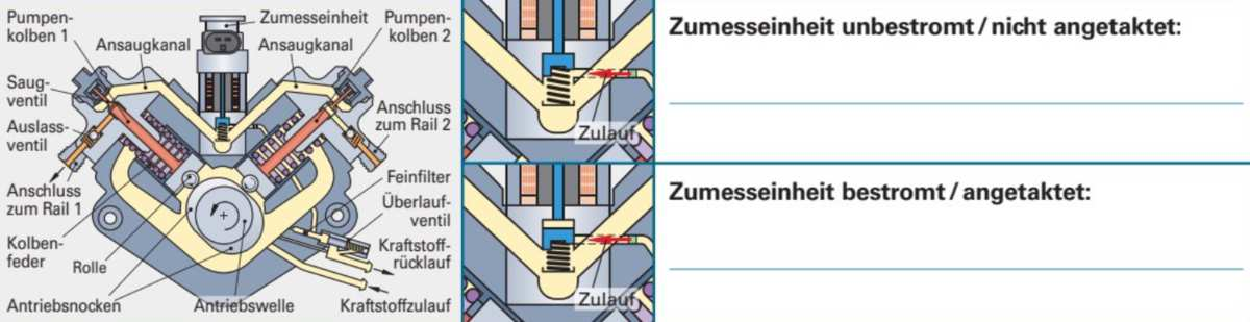
\includegraphics[width=0.8\textwidth]{images/Diesel/Diesel-3.pdf}
\caption{CR-Zumesseinheit, Quelle: Europa-Verlag}
%\label{fig:}%% anpassen
\end{figure}

\begin{enumerate}
\item
  \textbf{Zumesseinheit unbestromt}: Maximale Fördermenge
\item
  \textbf{Zumesseinheit bestromt}: verringert den Öffnungsquerschnitt
  für minimale Fördermenge
\end{enumerate}

\textbf{Druckregelventil} Druckerfassung durch Membransensor am Rail
(Raildrucksensor)

\begin{figure}[!ht]% hier: !ht
\centering
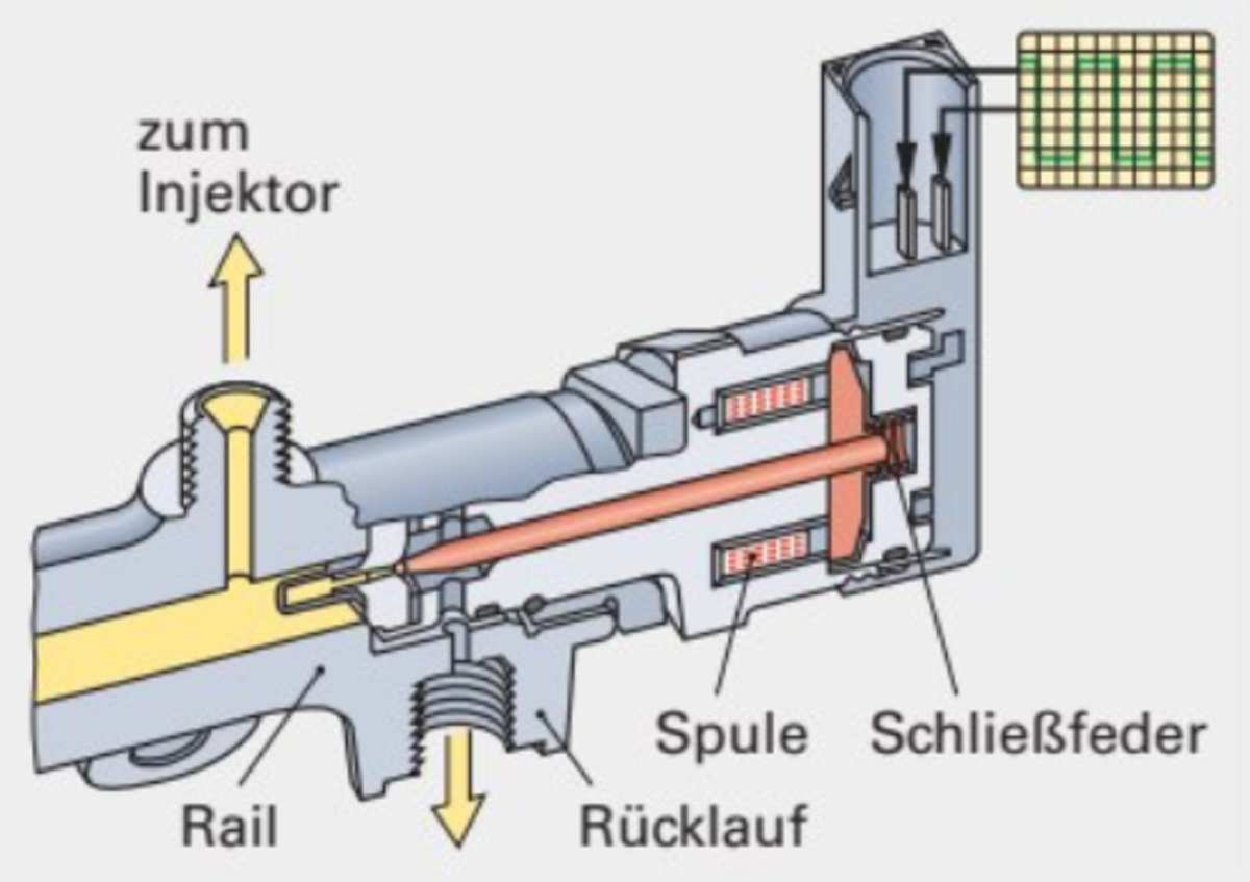
\includegraphics[width=0.3\textwidth]{images/Diesel/Diesel-8.pdf}
\caption{CR-Druckregelventil (DRV), Quelle: Europa-Verlag}
%\label{fig:}%% anpassen
\end{figure}

\emph{Ansteuerung:} Das Steuergerät taktet das Druckregelventil mit
einem PWM-Signal an. Dadurch wird die Schließkraft der Ventilnadel
erhöht oder gesenkt. Dementsprechend wird der Raildruck erhöht oder
gesenkt.

\begin{enumerate}
\item
  \textbf{Magnetventil unbestromt / stromlos} Raildruck etwa
  $100~\text{bar}$

  \begin{itemize}
  \item
    Motor abstellen, Ventilfeder hält Druckregelventil geschlossen,
    verhindert ein Leerlaufen des Rails
  \end{itemize}
\item
  \textbf{Magnetventil bestromt} Raildruck bei verschiedene
  Lastzuständen:

  \begin{itemize}
  \item
    \textbf{Motorstart} Raildruck $> 250~\text{bar}$ (Wie hoch ist der
    Druck im Rail bei Motorstart?)
  \item
    \textbf{Leerlauf} Raildruck etwa $400~\text{bar}$
  \item
    \textbf{Volllast} Raildruck etwa $2000~\text{bar}$
  \end{itemize}
\end{enumerate}

\newpage

\textbf{Warum lässt sich ein Fahrzeug mit defektem Druckregelventil
nicht mehr starten?}

\begin{figure}[!ht]% hier: !ht
\centering
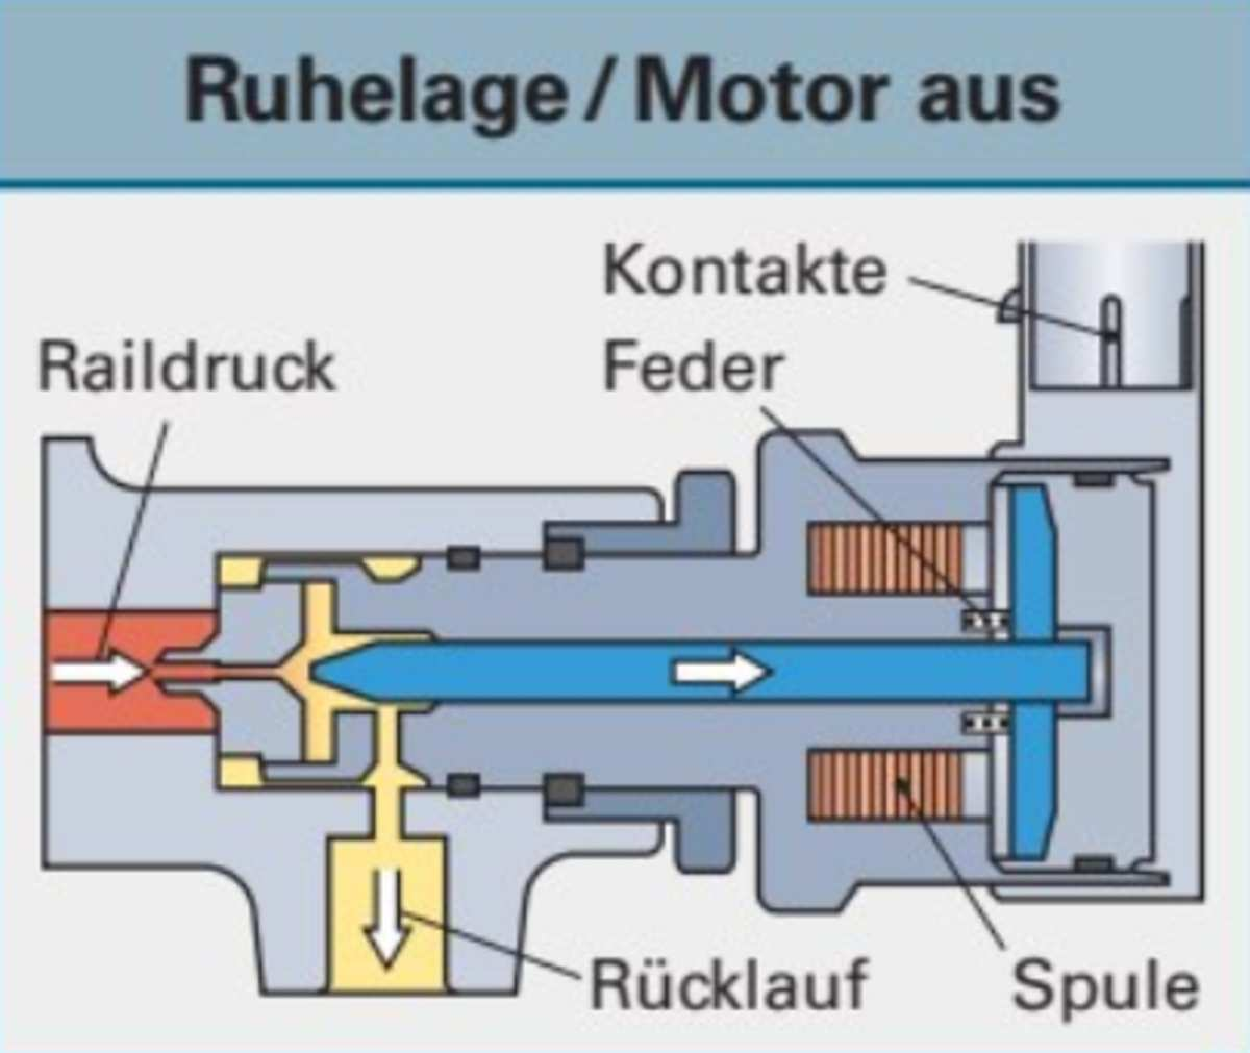
\includegraphics[width=0.3\textwidth]{images/Diesel/Diesel-4.pdf}
\caption{CR-DRV Motor aus, Quelle: Europa-Verlag}
%\label{fig:}%% anpassen
\end{figure}

Durch die im Druckregelventil verbaute Feder verbleibt im Rail ein
\textbf{Restdruck} von ca. 100 bar. Da für einen \textbf{sicheren
Motorstart} der Druck im Rail mind. 250 bar betragen muss, ist ein
Motorstart nicht möglich.

Ist die \textbf{ZME} defekt, übernimmt das \textbf{DRV} die
Druckregelung.

\newpage

\section{Injektoren}\label{injektoren}

\textbf{Unterschied zwischen Injektoren und Einspritzdüsen} haben keinen
festen Öffnungsdruck, sondern öffnen und schließen unter dem jeweiligen
variablen Einspritzdruck.

Kraft = Druck x Fläche

\subsection{Erklären Sie die Funktionsweise eines Magnetventil-Injektor
im geschlossenen und geöffneten
Zustand.}\label{erklaeren-sie-die-funktionsweise-eines-magnetventil-injektor-im-geschlossenen-und-geoeffneten-zustand.}

\begin{figure}[!ht]% hier: !ht
\centering
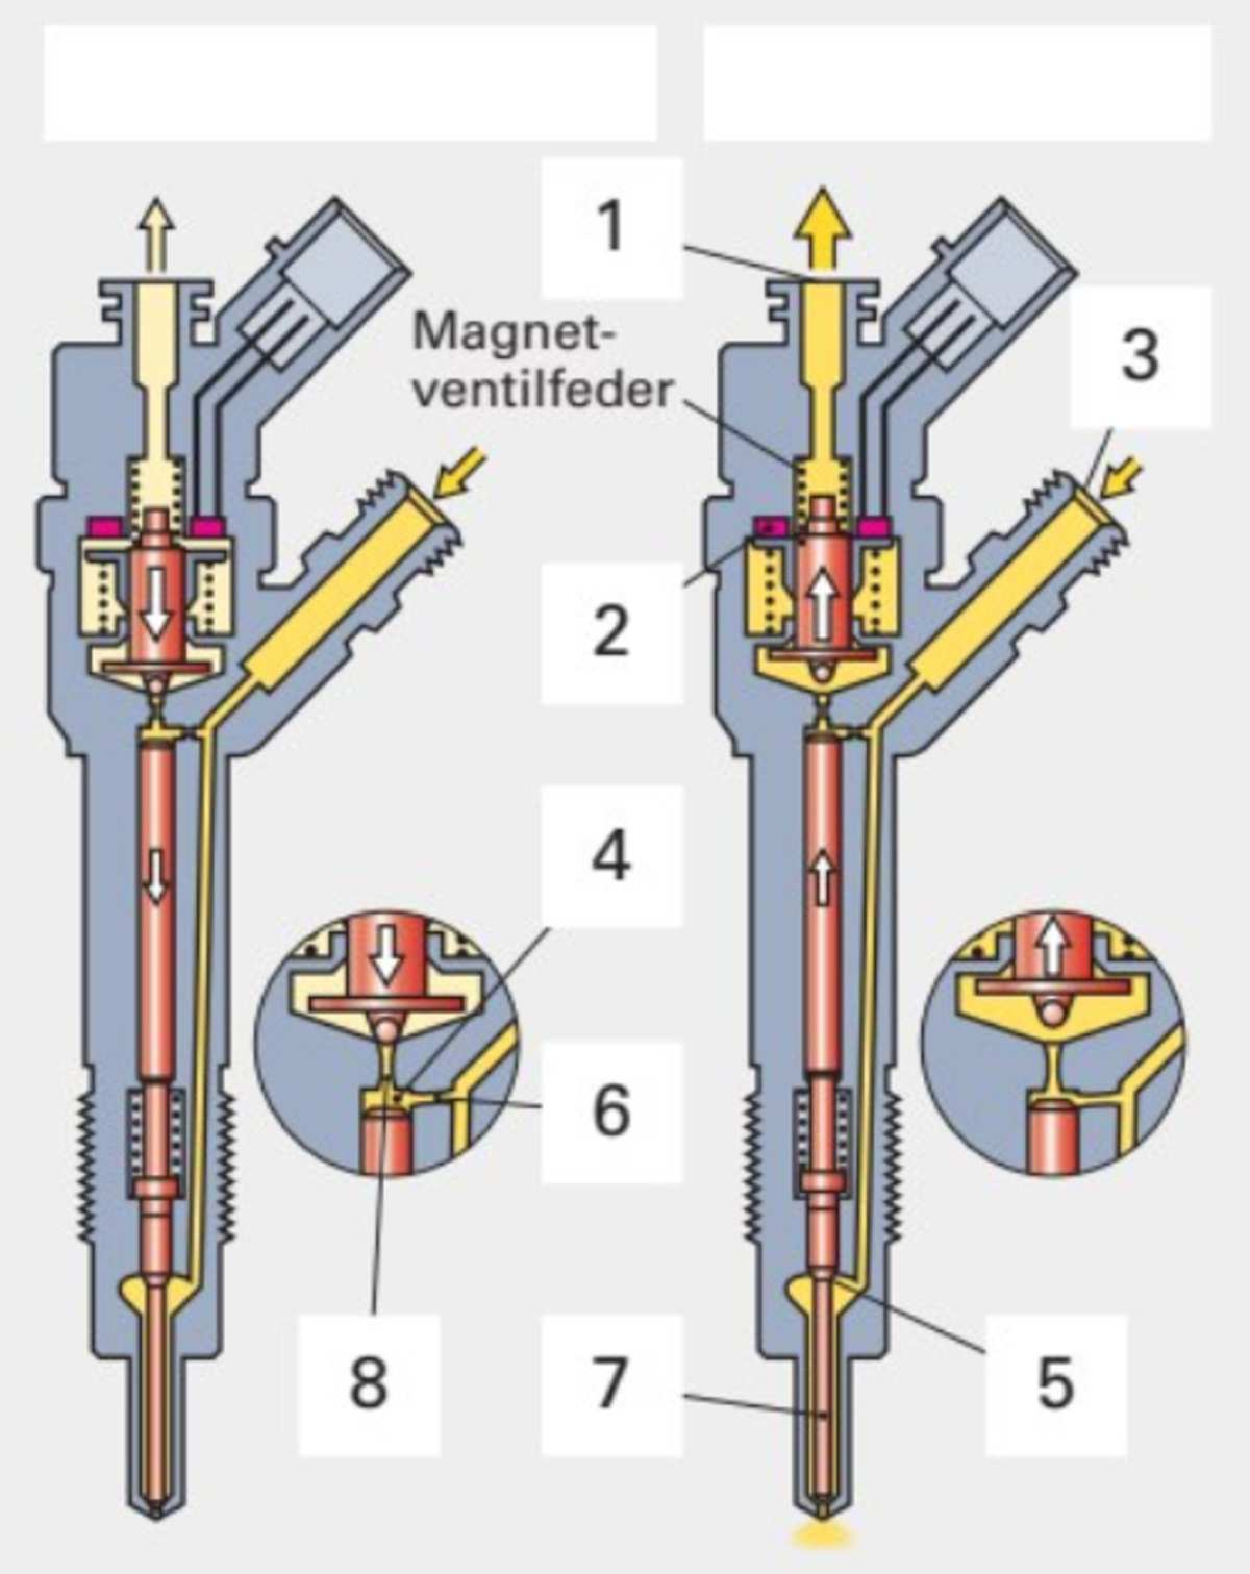
\includegraphics[width=0.3\textwidth]{images/Diesel/Diesel-7.pdf}
\caption{CR-Magnetventil-Injektor, Quelle: Europa-Verlag}
%\label{fig:}%% anpassen
\end{figure}

\begin{enumerate}
\item
  Rücklauf
\item
  Magnetventil
\item
  Zulauf von dem Rail
\item
  Ventilsteuerraum
\item
  Druckschulter
\item
  Zulaufdrossel
\item
  Düsennadel
\item
  Abflussdrossel
\end{enumerate}

\begin{itemize}
\item
  \textbf{Magnetventil unbestromt - geschlossenen Zustand} dann wirkt im
  Ventilsteuerraum auf der Stirnfläche des Ventilsteuerkolbens und auf
  der Druckschulter der Düsennadel gleicher Kraftstoffdruck.
  Einspritzventil ist geschlossen.
\item
  \textbf{Magnetventil bestromt - geöffneten Zustand,} dann wird der
  Rücklauf geöffnet. Über die Ablaufdrossel entweicht mehr Kraftstoff,
  als über die Zulaufdrossel abfließen kann. Es kommt zum Druckabfall im
  Ventilsteuerraum. Der Druck auf die Druckschulter der Düsennadel
  öffnet die Düse.
\end{itemize}

\textbf{Ansteuerung eines Magnetventil-Injektors (Spannungs- und
Stromverlauf)}

Die Injektorspannung / Boosterspannung beträgt in der Anzugsphase ca.
100 V. Der Anzugsstrom liegt dadurch bei ca. 20 A. Danach wird der Strom
auf ca. 13 A begrenzt (Haltestrom), bei einer Spannung von 12 -- 14 V
(Batteriespannung).

\textbf{Wie entsteht die Injektorspannung / Boosterspannung bis ca. 100
V?}

Beim Ausschalten der Magnetventile wird die entstehende
Selbstinduktionsspannung genutzt, um im Steuergerät einen Kondensator
aufzuladen.

\newpage

\subsection{Erklären Sie die Funktionsweise eines
Piezoinjektor}\label{erklaeren-sie-die-funktionsweise-eines-piezoinjektor}

Piezoinjektoren erlauben hohe Schaltgeschwindigkeiten und damit viele
Teileinspritzungen.

\begin{figure}[!ht]% hier: !ht
\centering
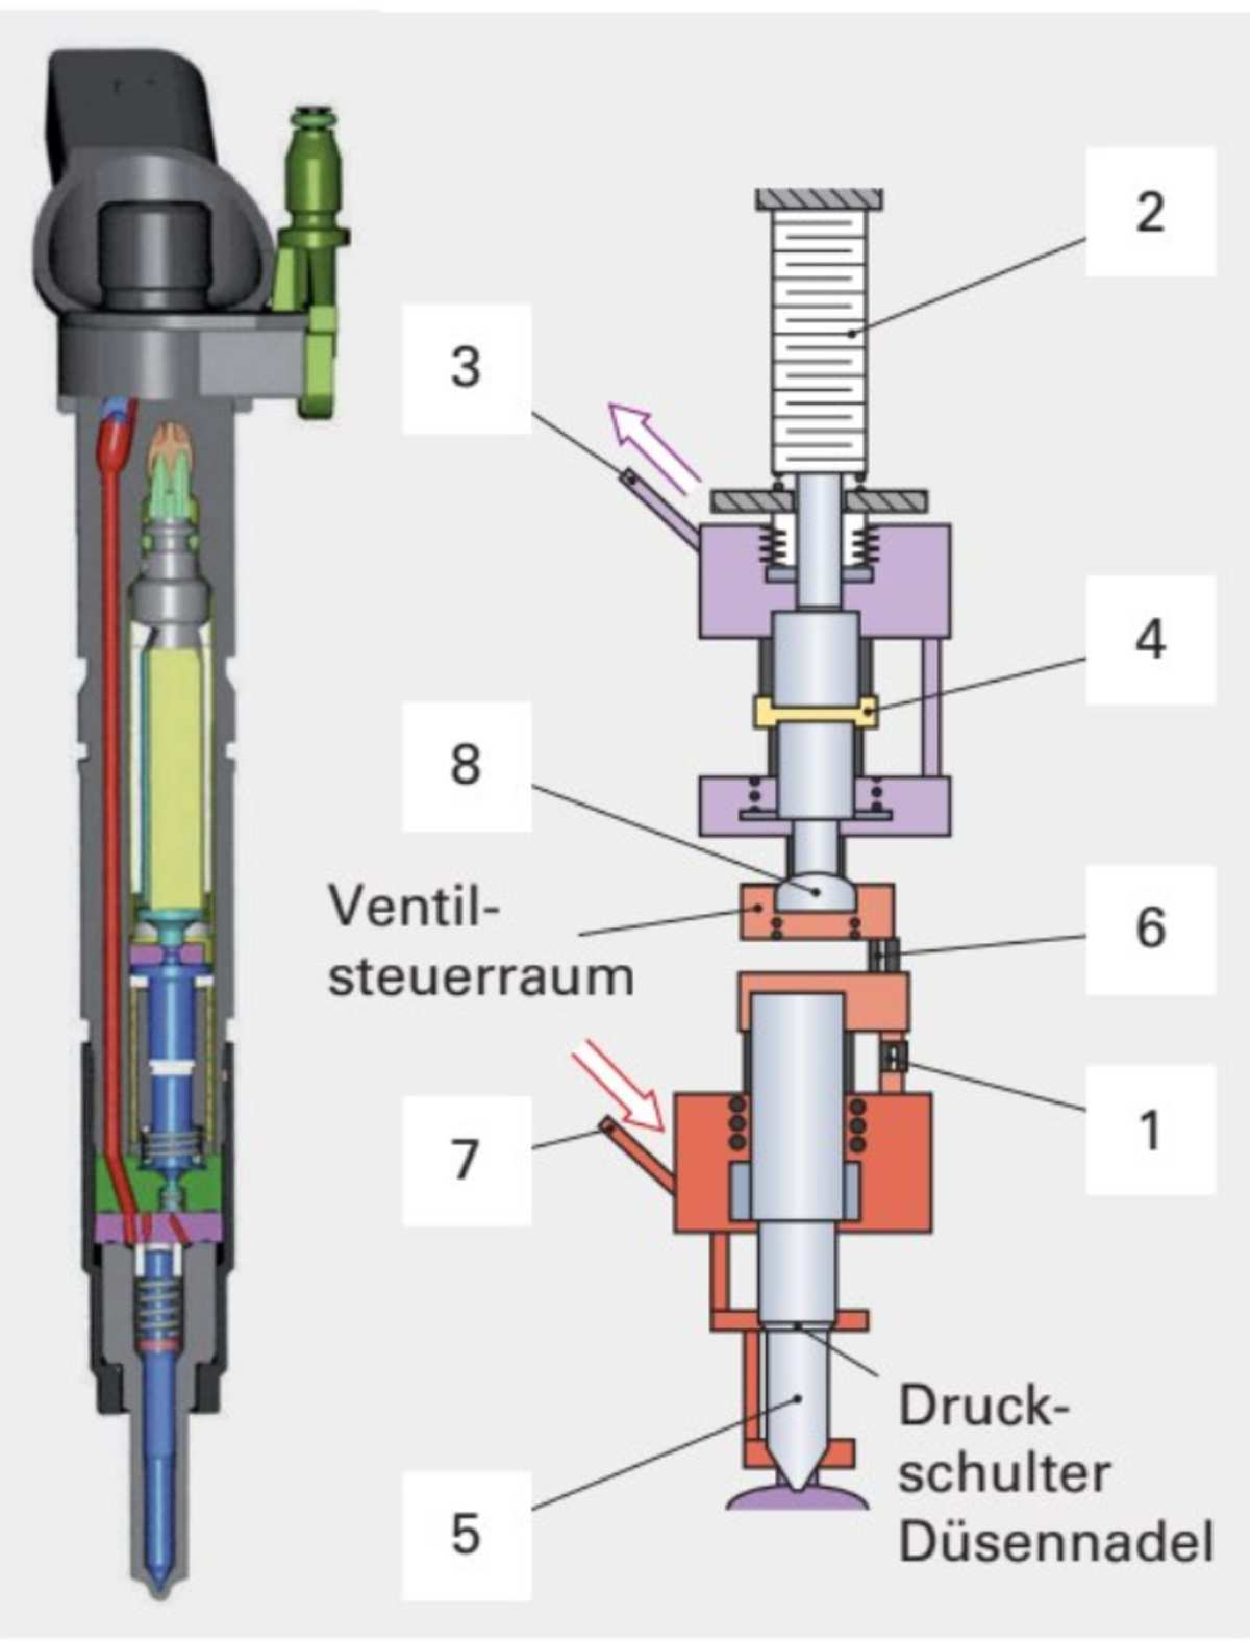
\includegraphics[width=0.3\textwidth]{images/Diesel/Diesel-1.pdf}
\caption{CR-Piezoinjektor, Quelle: Europa-Verlag}
%\label{fig:}%% anpassen
\end{figure}

\begin{enumerate}
\item
  Zulaufdrossel
\item
  Piezo-Aktormodul
\item
  Rücklauf
\item
  Hydraulischer Koppler
\item
  Düsennadel
\item
  Ablaufdrossel
\item
  Zulauf mit Raildruck
\item
  Servoventil
\end{enumerate}

\textbf{Einspritzvorgang}

\begin{enumerate}
\item
  Piezo-Aktormodul wird bestromt und dehnt sich aus
\item
  Über den hydraulischen Koppler findet eine Hubvergrößerung statt.
\item
  Der hydraulischen Koppler öffnet das Servoventil und damit den
  Rücklauf.
\item
  Über die Ablaufdrossel fließt Kraftstoff aus dem Ventilsteuerraum ab.
\item
  Über die Zulaufdrossel kann weniger Kraftstoff in den Ventilsteuerraum
  zufließen. Es kommt zum Druckabfall.
\item
  Der Druck auf die Druckschulter der Düsennadel öffnet die Düsennadel
  des Injektors. Einspritzbeginn.
\end{enumerate}

\textbf{Hydraulische Koppler vergrößert den Weg des Piezo-Aktormoduls
auf das Servoventil}

\begin{figure}[!ht]% hier: !ht
\centering
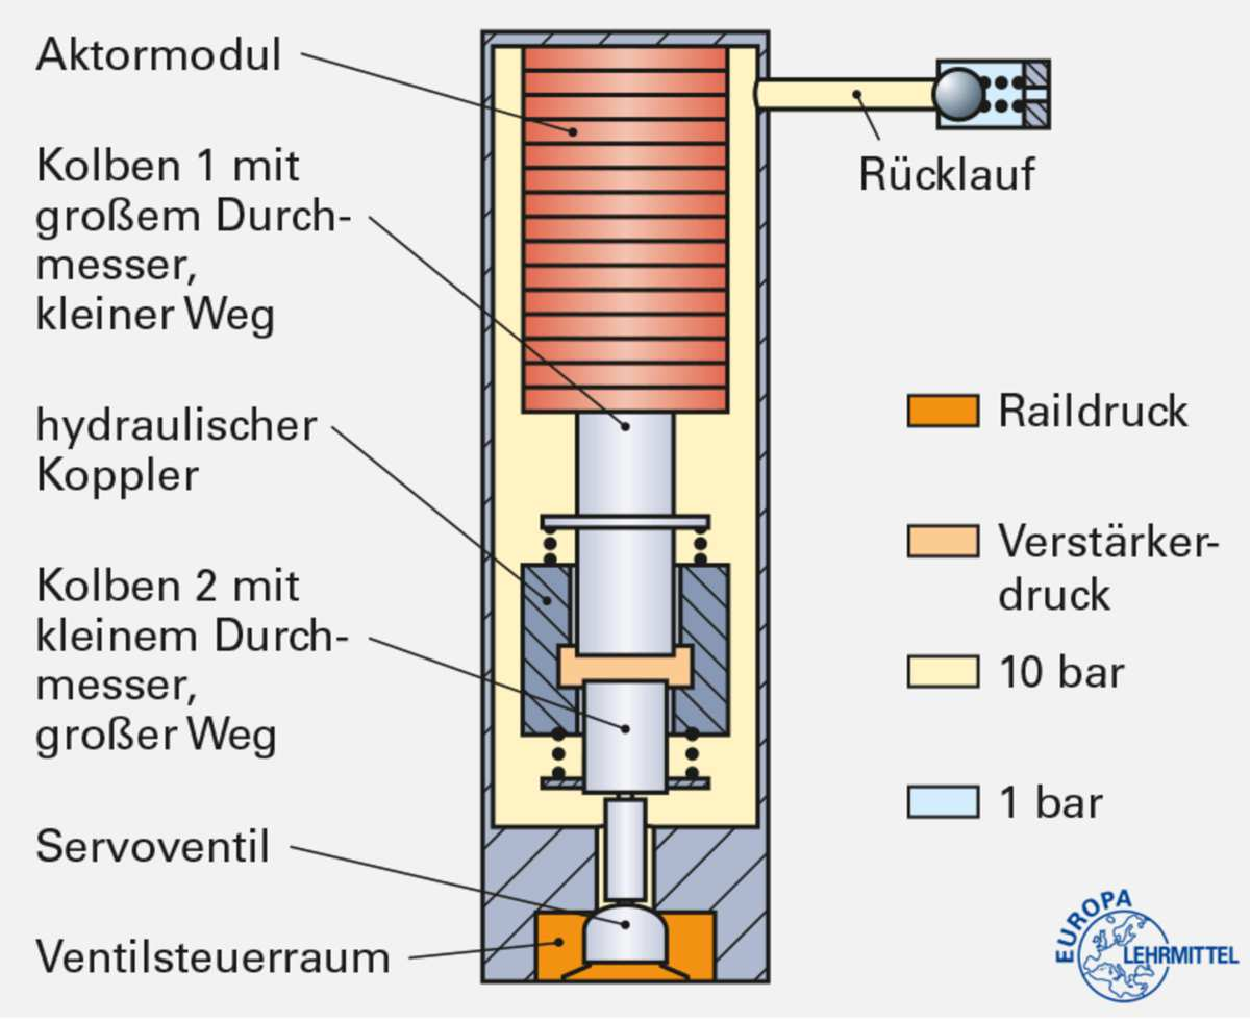
\includegraphics[width=0.3\textwidth]{images/Diesel/Diesel-21.pdf}
\caption{CR-Piezoinjektor - hydraulicher Koppler, Quelle: Europa-Verlag}
%\label{fig:}%% anpassen
\end{figure}

Er besteht aus zwei Kolben mit unterschiedlichen Durchmessern. Das
Piezo-Aktormodul drückt mit kleinem Hub auf den großen Kolben, dadurch
wird der kleine Kolben mit einem großen Hub bewegt.

\textbf{Reziproker Piezoelektrischer-Effekt} (invers) legt man an einen
Piezokristall eine Spannung an, so verformt er sich. Die Längenänderung
ist proportional zur angelegten Spannung. Bleibt in Position bis
Kurzschluss.

\emph{Verformung} durch Spannungseinfluss

\emph{Anwendung:} Injektor

\textbf{Ansteuerung eines Piezoinjektors} 110 -- 150 V bei ca. 13 A,
Piezoaktormodul dehnt sich aus (am Ende vergleichbar mit geladenen
Kondensator) \emph{Injektor offen:} Stromaufnahme null \emph{Injektor
geschlossen:} SG schaltet Spannung ab und schließt Stromkreis über
Widerstand kurz. Piezoaktormodul entlädt sich und zieht sich zusammen.

Piezoventil ersetzt Magnetventil (Grund: durch Trägheit $\to$
Magnetventil bewegt sich zeitversetzt, weil der Magnetfeldaufbau gehemmt
wird, durch Gegeninduktion)

\textbf{Piezoventil (Piezoaktor)} besteht aus Piezoaktormodul und
Übersetzermodul (kl. Hebelwerk)

Die Längenausdehnung eines Piezokristalls liegt bei maximal 0,15 \%
(sehr gering). Werden, bis zu 500 Piezokristalle in Reihe geschaltet ist
die Gesamtausdehnung des Piezoaktormodul etwa 0,04 mm. Zum Erreichen der
erforderlichen Ventilöffnung von 0,1 mm wird ein kleines Hebelwerk,
sogenannte Übersetzermodul zwischen Piezoaktormodul und hydraulischen
Ventil geschaltet.

\chapter{09-Loesung-Common-Rail-Diesel-II}
%%ju 31-Dez-22 09-Loesung-Common-Rail-Diesel-II.tex
\textbf{1) Beschreiben Sie ausführlich den Einspritzvorgang beim
Pumpe--Düse--System mit Magnetventil.}

\textbf{Befüllen} bei ablaufenden Einspritznocken wird der Pumpenkolben
nach oben gezogen und der Hochdruckraum wird mit Kraftstoff befüllt.
Solange Magnetventil offen ist, fließt der Kraftstoff durch den
Hochdruckraum in den Rücklauf ab. (kühlende Wirkung) Bei auflaufenden
Nocken wird der Pumpenkolben nach unten gedrückt. Magnetventil ist
geschlossen und verschließt Kraftstoff, Vor- und Rücklaufleitung. Es
baut sich ein Hochdruck auf.

\textbf{Voreinspritzung} (Beginn) bei etwa 180 bar ist der Druck größer
als die Düsen-Federkraft. Durch das Einspritzen des Kraftstoffs haben
wir einen kurzen Druckabfall und die Düsennadel schließt (Ende). Der
Ausweichkolben hat seine schräge Druckschulter freigegeben (große
Fläche, große Kraft), wodurch er nach unten gedrückt wird und spannt die
Düsenfeder vor. Magnetventil öffnet und der überschüssige Kraftstoff
entweicht in die Vor- und Rücklaufleitung.

\textbf{Haupteinspritzung} der Druck steigt weiter und drückt bei etwa
300 bar die Düsennadel nach oben (Ende). Durch den Druckabfall schließt
die Düsennadel.

\textbf{2) Wie lässt sich beim Pumpe--Leitung--Düse--System eine
Voreinspritzung realisieren?} (NFZ)

Durch Zweifeder-Düsenhalter (kleine Feder - Voreinspritzung, große Feder
- Haupteinspritzung). Bei geringem Kraftstoffdruck öffnet die Düse nur
teilweise.

\textbf{3) Welche Hauptvorteile bietet das Common--Rail--System
gegenüber allen anderen gängigen Einspritzsystemen?}

\begin{itemize}
\item
  Einspritzmenge lässt sich über Zeit und Einspritzdruck variieren (je
  nach Betriebszustand)
\item
  Kein Druckanstieg im Einspritzvorgang: (der Öffnungsdruck entspricht
  dem jeweiligen Einspritzdruck)
\item
  beliebige Anzahl von Einspritzvorgängen (ruhigen Motorleerlauf viele
  Einspritzungen, für maximales Drehmoment bei Volllast nur eine)
\item
  Einspritzung unabhängig von Kurbelwellen- und Nockenwellenposition
  (Kraftstoffdruck steht immer an)
\item
  Anpassung an unterschiedliche Motoren
\end{itemize}

\textbf{4) Welche Regelungsarten des Common--Rail--Systems kennen Sie?}

\begin{enumerate}
\item
  \textbf{Einsteller-Regelung}

  \begin{itemize}
  \item
    \textbf{Druckregelung hochdruckseitig} über ein
    \textbf{Druckregelventil} (DRV)

    \begin{itemize}
    \item
      Hochdruckpumpe fördert die maximale Fördermenge unabhängig von
      Bedarf an Kraftstoff
    \item
      Raildruck wird über ein \textbf{Druckregelventil} geregelt, nicht
      benötigter Kraftstoff fließt zurück in den Tank
    \item
      \textbf{Vorteil}

      \begin{itemize}
      \item
        schneller Druckaufbau möglich
      \item
        bei Lastwechsel agil
      \end{itemize}
    \item
      \textbf{Nachteil:} Hochdruckpumpe ist, konstant maximal belastet,
      dadurch

      \begin{itemize}
      \item
        geringere Nutzleistung
      \item
        erhöhter Kraftstoffverbrauch, Schadstoffausstoß, Verschleiß
      \item
        unnötige Erwärmung des Kraftstoffs
      \end{itemize}
    \end{itemize}
  \item
    \textbf{Druckregelung niederdruckseitig} (Mengenregelung) über eine
    \textbf{Zumesseinheit} (ZME)

    \begin{itemize}
    \item
      \textbf{Zumesseinheit} regelt die Zuflussmenge zur Hochdruckpumpe
    \item
      \textbf{Bedarfsregelung}, d.h. es gelangt nur so viel Kraftstoff
      zu Hochdruckpumpe wie für die Einspritzung benötigt wird
    \item
      \textbf{Druckbegrenzungsventil} verhindert zu hohen Raildruck bei
      Ausfall der Zumesseinheit
    \item
      \textbf{Vorteil}

      \begin{itemize}
      \item
        bedarfsgerechte Förderung
      \item
        Reduzierte Leistungsaufnahme der Pumpe
      \end{itemize}
    \item
      \textbf{Nachteil:}

      \begin{itemize}
      \item
        hohe Trägheit
      \item
        Drucksteigerung erfordert zunächst eine Erhöhung des
        Niederdrucks, dadurch erhöhte Förderleistung der Hochdruckpumpe
      \end{itemize}
    \end{itemize}
  \end{itemize}
\item
  \textbf{Zweisteller-Regelung} (\textbf{Druckregelung nieder- und
  hochdruckseitig})

  \begin{itemize}
  \item
    Zusammenspiel von Zumesseinheit (ZME) und Druckregelventil (DRV)
  \item
    \textbf{Vorteile}

    \begin{itemize}
    \item
      geringe Leistungsaufnahme der Hochdruckpumpe bei konstant hohen
      Drücken
    \item
      hohe Agilität bei geringen Drücken
    \end{itemize}
  \item
    \textbf{Kaltstart / Motorstart und Warmlaufphase} (angesteuert:
    \textbf{DRV}) >>Druckregelung hochdruckseitig geregelt<<

    \begin{itemize}
    \item
      Schneller Druckaufbau möglich. Bessere Kraftstoffvorwärmung.
      Verzicht auf Kraftstoffheizung möglich.
    \item
      Kraftstoff soll sich erwärmen, um ihn damit fließ- und zündfähiger
      zu machen
    \end{itemize}
  \item
    \textbf{betriebswarmer Motor: Leerlauf / Teilllast / Schub}
    (angesteuert: \textbf{DRV und ZME}) >>Zweisteller-Betrieb<<

    \begin{itemize}
    \item
      große Sprünge des Raildrucks sind wahrscheinlich (zwischen Motor
      im Leerlauf / Teillast und $\to$ Lastwunsch des Fahrers bei
      Volllast)
    \item
      Raildruckregelung bei reduzierter Leistungsaufnahme der Pumpe
    \end{itemize}
  \item
    \textbf{hohen Motorlast} (angesteuert: \textbf{ZME}) >>Druckregelung
    niederdruckseitig geregelt<<

    \begin{itemize}
    \item
      große Steigerungen des Raildrucks nicht möglich und deshalb ist
      die Trägheit vernachlässigbar
    \item
      Reduzierter Leistungsaufnahme der Pumpe. Gesamte Kraftstoffmenge
      der Pumpe wird eingespritzt.
    \end{itemize}
  \end{itemize}
\end{enumerate}

\textbf{5) Was passiert, wenn das Druckregelventil eines
Common--Rail--Systems ausfällt?}

Da das Druckregelventil im spannungsfreien Zustand nur ca. 100 bar
halten kann, der CR-Motor aber, um anzuspringen, 250 bar benötigt, läuft
der Motor bei Ausfall des Druckregelventils nicht.

\textbf{6) Warum wird der Druck in der Rail bei kaltem Motor
ausschließlich über das Druckregelventil geregelt?}

Um den Kraftstoff schneller zu erwärmen, um ihn damit fließ- und
zündfähiger zu machen.

\textbf{7) Welche Spannung ist zum Öffnen eines Magnetspuleninjektors
notwendig? Wie wird diese erzeugt?}

Um den Magnetventilspuleninjektor zu öffnen, wird eine Spannung von ca.
100 V bei einer Stromstärke von 20 A benötigt. Diese entsteht als
Selbstinduktionsspannung im Abschaltmoment des Injektors und wird im
Steuergerät in sogenannten Boosterkondensatoren gespeichert. Sind die
Boosterkondensatoren entladen, kann das Steuergerät die Entstehung einer
Selbstinduktionsspannung provozieren, in dem es die Injektoren mehrfach
mit Bordnetzspannung an taktet, wodurch diese zwar nicht öffnen, jedoch
die erforderliche Selbstinduktionsspannung entstehen kann.

\textbf{8) Welche Vorteile bietet der Piezoinjektor gegenüber dem
Magnetspuleninjektor? Erläutern Sie den technischen Hintergrund.}

Während die Anzahl der Einspritzvorgänge pro Arbeitstakt beim
Magnetspuleninjektor auf maximal fünf begrenzt ist, da es bei jeden
Magnetfeldaufbau in ihm zu einer Gegeninduktion kommt, die den
Magnetfeldaufbau hemmt und den einzelnen Einspritzvorgang damit
verlangsamt, kann der Piezoinjektor problemlos sieben und mehr
Einspritzvorgänge pro Arbeitstakt realisieren.

\textbf{9) Beschreiben Sie den Aufbau einer elektronisch geregelten
Glühstiftkerze. Wie schafft man es, dass diese Glühkerze deutlich
schneller auf Glühtemperatur ist, als die herkömmliche Glühkerze?}

Die elektronisch geregelte Glühstiftkerze besteht wie auch die
herkömmlich Selbstregelnde Glühkerze aus einer Heiz- und einer
verkürzten Regelwendel. Sie besitzt allerdings nur eine Nennspannung von
5 -- 8 V, um die Glühkerze besonders schnell auf Glühtemperatur zu
bekommen, wird sie durch ein PWM-Signal kurzzeitig mit ca. 11 V
angesteuert, also eigentlich überlastet. Hierdurch erreicht sie binnen 1
-- 2 Sekunden eine Glühtemperatur von bis zu $1000^\circ\text{C}$
bevor das Tastverhältnis, das PWM-Signal so weit verändert, dass an der
Glühkerze nur ihre Nennspannung anliegt. Die ausreichend ist, um sie auf
Temperatur zu halten.

\textbf{10) Welche Möglichkeiten der Motor- und Innenraum-Zuheizung
kennen Sie. Nennen Sie Vor- und Nachteile der einzelnen Systeme.}

\begin{table}[!ht]% hier: !ht 
\centering 
	\caption{}% \label{tab:}%% anpassen 
\begin{tabular}{@{}lcccc@{}}
\hline
\textbf{System} & \textbf{Innenraum} & \textbf{Innenraum + Motor} &
\textbf{Energie} & \textbf{Kühlen} \\
\hline
Kraftstoff-Zuheizer & & \checkmark & \checkmark & \\
PTC-Heizung & \checkmark & & \checkmark & \\
Elektrisches Zuheizsystem & & \checkmark & \checkmark & \\
Abgas-Wärmetauscher & \checkmark & & & \\
Wassergekühlter Generator & & \checkmark & & \checkmark \\
Kraftstoff-Wärmetauscher & & \checkmark & & \checkmark \\
\hline
\end{tabular} 
\end{table}

\textbf{Motorzuheizung} nach Motorstart wird beheizt.

(\textbf{Standheizung} ca. 10 Minuten vorheizen, bei Motorstart schon
warm.)

\chapter{10-Kuehlsystem}
%%ju 26-Dez-22 10-Kuehlsystem.tex
\textbf{Welche Aufgabe hat das Kühlsystem eines Verbrennungsmotors?}

\begin{enumerate}
\item
  schnelle Erwärmung des Motors auf Betriebstemperatur
\item
  überschüssige Wärme muss schnell und zuverlässig abgeleitet werden
\end{enumerate}

\textbf{Betriebstemperatur}

Kühlmitteltemperaturen zwischen $80 - 120^\circ\text{C}$

Überdruck im Kühlsystem: Pkw: 1,3 -- 2 bar, Nfz: 0,5 -- 1,1 bar (bessere
Kühlung, erfordert Ausgleichsbehälter)

\textbf{Ziel: schnelles Erreichen der Betriebstemperatur des Motors}

$\to$ geringerer Kraftstoffverbrauch und Schadstoffemissionen

\section{Anforderungen an das
Kühlsystem}\label{anforderungen-an-das-kuehlsystem}

\begin{enumerate}
\item
  ausreichende Kühlwirkung
\item
  schnelles Erreichen der Betriebstemperatur
\item
  geringes Gewicht
\item
  gleichmäßige Kühlung der Bauteile, um Wärmespannung zu vermeiden
\item
  geringer Energiebedarf für den Betrieb des Kühlsystems
\end{enumerate}

\emph{Eine gute Kühlung ermöglicht somit} $\dots$

\begin{enumerate}
\item
  verbesserte Zylinderfüllung
\item
  verminderte Klopfneigung bei Ottomotoren
\item
  höhere Verdichtung
\item
  höhere Leistung
\item
  geringerer Kraftstoffverbrauch
\item
  gleichmäßige Betriebstemperaturen
\end{enumerate}

\section{Welche Kühlungsarten werden
unterschieden?}\label{welche-kuehlungsarten-werden-unterschieden}

\begin{enumerate}
\item
  \textbf{Luftkühlung} (Fahrtwindkühlung, Gebläseluftkühlung)

  \begin{itemize}
  \item
    $\to$ Wärme wird direkt an die umströmende Umgebungsluft abgegeben
  \item
    Nachteil: größere Schwankungen der Betriebstemperatur
  \end{itemize}
\item
  \textbf{Flüssigkeitskühlung} (Pumpenumlaufkühlung,
  Zwangsumlaufkühlung)

  \begin{itemize}
  \item
    $\to$ Kühlmittel nimmt die Wärme auf und gibt sie durch den Kühler
    an die Umgebungsluft ab
  \item
    Vorteil: gleichmäßige Kühlwirkung, Motortemperaturregelung
  \end{itemize}
\item
  \textbf{Innenkühlung des Brennraums} (Verdampfung des Kraftstoffs)

  \begin{itemize}
  \item
    $\to$ Energie aufnehmen - aus der Umgebung wird Wärme entzogen.
  \item
    Notwendig, wenn man eine Flüssigkeit verdampfen möchte. (flüssig
    $\to$ gasförmig, Druck ist konstant)
  \end{itemize}
\end{enumerate}

\section{Additive für Kühlmittel}\label{additive-fuer-kuehlmittel}

\begin{itemize}
\item
  Konditioniertes Kühlmittel (Gemisch aus Wasser und Frostschutzmittel -
  bekannt als Glysantin, Ethylenglykolbasis G11/12, Propylenglykolbasis
  G13)
\item
  Korrosionsinhibitoren (Hemmstoff, Schutz vor Korrosion)
\item
  Schutz gegen Kesselstein (Kalkablagerung)
\item
  Neutralisationsmittel gegen Ameisen- und Essigsäure
\item
  Kavitation Schutzmittel (Dampfblasen)
\item
  Antischaumbildner
\end{itemize}

\section{Kavitation (lat. cavitare, aushöhlen, Hohlsog, Abtragen von
Werkstoff)}\label{kavitation-lat.-cavitare-aushoehlen-hohlsog-abtragen-von-werkstoff}

\textbf{Kavitation} wird der Dampfdruck (Mischung aus einem Gas und
einer Flüssigkeit) einer Flüssigkeit unterschritten, kommt es zur
Bildung von Gasblasen, die beim Wiederanstieg des Drucks implodieren und
einen Flüssigkeitsstrahl (Micro-Jet) auslösen.

Micro-Jet haben einen Durchmesser von etwa $1~\mu m$ und treffen mit
bis zu 1000 m/s auf das Bauteil, wo er das Material mit einem Druck von
bis zu 100 000 bar verdichtet. Was zur Folge hat, dass das Material
spröde wird und beginnt sich auszulösen (Lochfraß).

\textbf{Kavitationsarten}

\begin{enumerate}
\item
  \textbf{Strömungskavitation}, die Dampfblasenbildung wird durch einen
  Druckabfall im Bereich der Umwälzpumpe oder Engstellen bzw. Kanten im
  Kreislauf ausgelöst.
\item
  \textbf{Schwingungskavitation}, die Dampfblasenbildung wird durch das
  Schwingen von Bauteilen und dem daraus resultierenden Druckabfall beim
  Entfernen des Flüssigkeitsmantels ausgelöst.

  \begin{itemize}
  \item
    Großdieselmotoren z. B. Schiffsmotor (an der Zylinderwand)
  \end{itemize}
\end{enumerate}

\textbf{Folgen der Kavitation:}

\begin{enumerate}
\item
  Material wird aushärten, porös und spröde
\item
  Materialausbrüche
\item
  Verformungen
\item
  Brüche
\item
  Löcher
\end{enumerate}

\textbf{Beispiele:}

\begin{enumerate}
\item
  \textbf{Kühlmittelpumpe}, durch einen Schaden am Überdruckventil oder
  die Dichtung des Verschlussdeckels vom Ausgleichsbehälter. Der
  Druckabfall im System ändert das Siedeverhalten des Kühlmittels und es
  kommt im Bereich größerer Druckgefälle (z. B. an der Kühlmittelpumpe -
  Saug- und Druckseite) zu einem Schaden.
\item
  \textbf{Schiffsschraube} Saug- und Druckseite, im Wechsel: Druck
  gering/hoch $\to$ Siedetemperatur fällt/steigt, Druckgefälle
  $\Delta p$

  \begin{itemize}
  \item
    vor der Schraube, Saugseite, niedriger Druck, Siedetemperatur fällt
  \item
    nach der Schraube, Druckseite, höherer Druck, Siedetemperatur steigt
  \end{itemize}
\end{enumerate}

\textbf{Ursachen für Kavitation:}

\begin{enumerate}
\item
  Druckabfall im System
\item
  Knicke in Schläuchen (Verengung)
\item
  Verstopfungen im System (Kesselstein, Kalkablagerung)
\end{enumerate}

\newpage

\section{Wärmemanagement -
Gesamtkühlkreislauf}\label{waermemanagement-gesamtkuehlkreislauf}

\begin{enumerate}
\item
  Motorkühlkreislauf
\item
  Motorölkühlkreislauf
\item
  Getriebeölkühlkreislauf (Automatikgetriebe)
\item
  Niedertemperaturkühlkreislauf (AGR-Rate)
\item
  Niedertemperaturkühlkreislauf (Ladeluft)
\end{enumerate}

\textbf{Thermostat} (Temperaturregler für Kühlmittel)

\begin{itemize}
\item
  Wasserumlauf über den Kühler wird in Abhängigkeit von der
  Kühlmitteltemperatur geregelt
\item
  Motor schnell seine Betriebstemperatur erreicht und konstant halten
  (geringe Schwankungen der Motortemperatur)
\item
  stufenloses Umschalten zwischen kleinem und großem Kühlkreislauf
\item
  Dehnstoffregler (Wachs) - über die Kühlmitteltemperatur wird das Wachs
  flüssig und dehnt sich aus. Diese Ausdehnung bewirkt einen Hub.
\item
  Dehnstoffelement (Wachselement) öffnet oder schließt die
  Steuerventile. (zum Kühler, Pumpe, vom Motor)
\item
  Sinkt die Temperatur des Kühlmittels, drückt eine Feder die Metalldose
  über den Kolben zurück und Ventil schließt den Durchfluss zum Kühler.
\end{itemize}

\begin{figure}[!ht]% hier: !ht
\centering
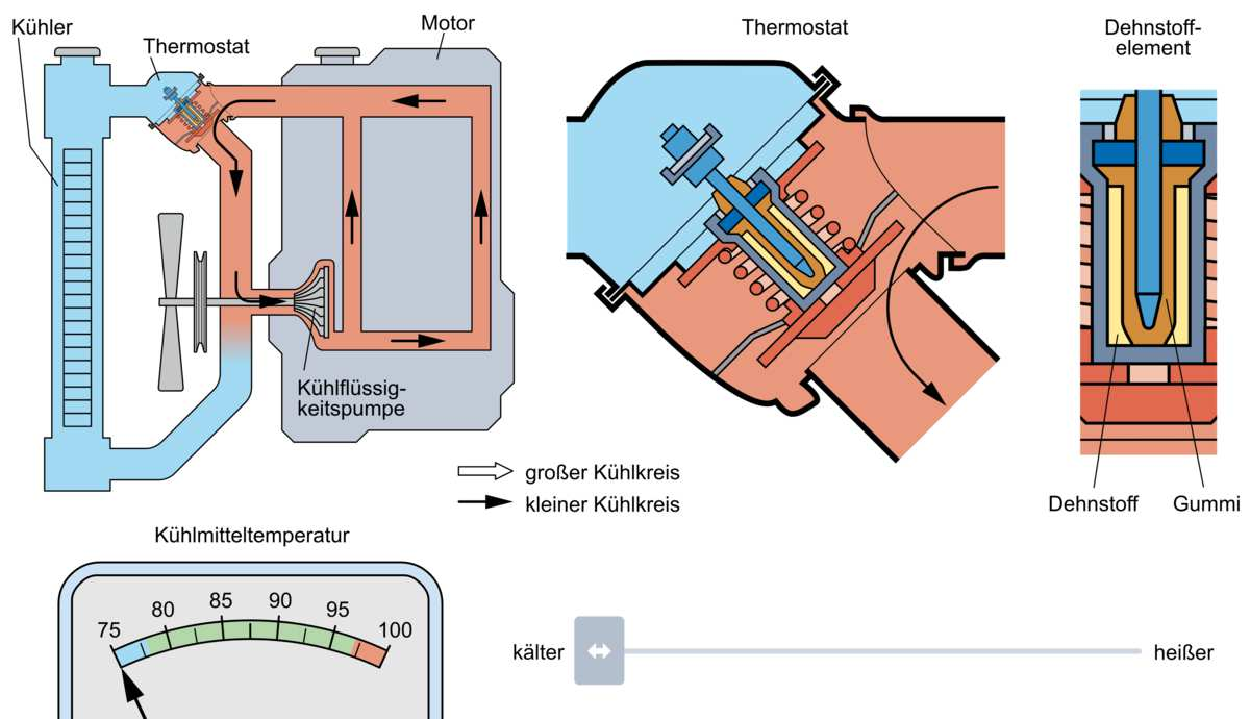
\includegraphics[width=0.5\textwidth]{images/Kuehlsystem/Kuehlsystem-5.pdf}
\caption{Thermostat - kalter Motor, Quelle: Europa-Verlag}
%\label{fig:}%% anpassen
\end{figure}

\begin{figure}[!ht]% hier: !ht
\centering
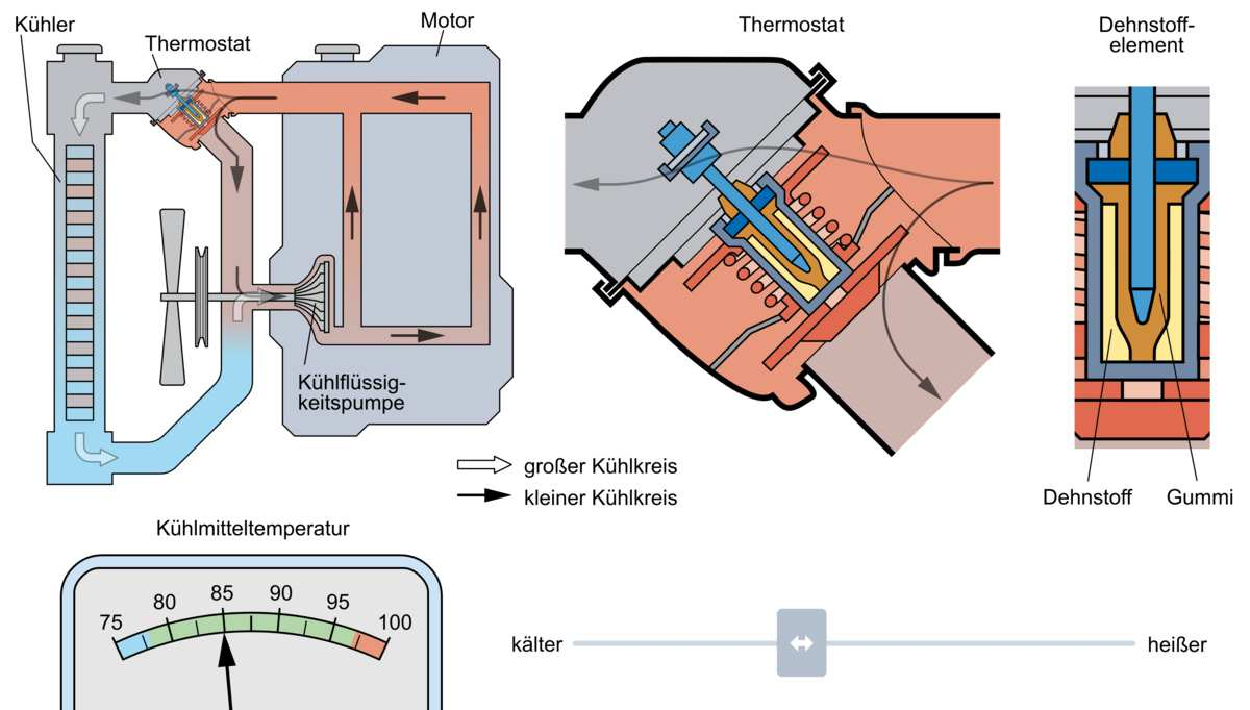
\includegraphics[width=0.5\textwidth]{images/Kuehlsystem/Kuehlsystem-6.pdf}
\caption{Thermostat - Kühlmitteltemperatur $85^\circ\text{C}$, Quelle:
Europa-Verlag}
%\label{fig:}%% anpassen
\end{figure}

\begin{figure}[!ht]% hier: !ht
\centering
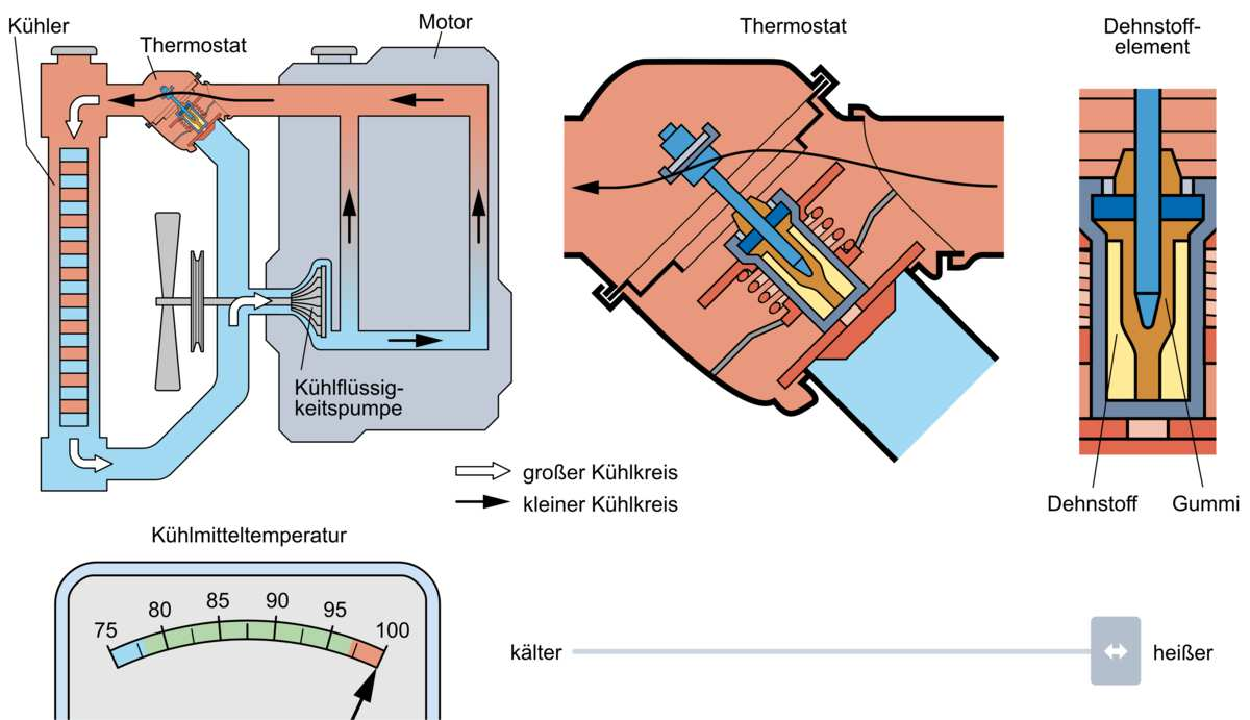
\includegraphics[width=0.5\textwidth]{images/Kuehlsystem/Kuehlsystem-7.pdf}
\caption{Thermostat - heißer Motor, Quelle: Europa-Verlag}
%\label{fig:}%% anpassen
\end{figure}

\begin{enumerate}
\item
  \textbf{Kleiner Kühlkreislauf} (kaltem Motor)

  \begin{itemize}
  \item
    Ventil geschlossen $\to$ kein Durchfluss zum Kühler
  \item
    \emph{Kreislauf:} Kühlmittelpumpe $\to$ Turbolader $\to$ Motor
    $\to$ Thermostat $\to$ Kühlmittelpumpe

    \begin{itemize}
    \item
      Bei Innenraumheizung: einen Teil des erwärmten Kühlmittels wird
      über Heizungswärmetauscher geführt
    \end{itemize}
  \end{itemize}
\item
  \textbf{großer Kühlkreislauf} (Betriebstemperatur)

  \begin{itemize}
  \item
    Ventil öffnet $\to$ Durchfluss zum Kühler (Kühlmitteltemperatur
    etwa $80^\circ\text{C}$)
  \item
    Ventil geöffnet $\to$ voller Durchfluss zum Kühler
    (Kühlmitteltemperatur etwa $95^\circ\text{C}$)
  \item
    \emph{Kreislauf:} Kühlmittelpumpe $\to$ Turbolader $\to$ Motor
    $\to$ Kühler $\to$ Thermostat $\to$ Kühlmittelpumpe
  \end{itemize}
\end{enumerate}

\newpage

\section{Elektronisches Wärmemanagement
(Kennfeldkühlung)}\label{elektronisches-waermemanagement-kennfeldkuehlung}

\begin{figure}[!ht]% hier: !ht
\centering
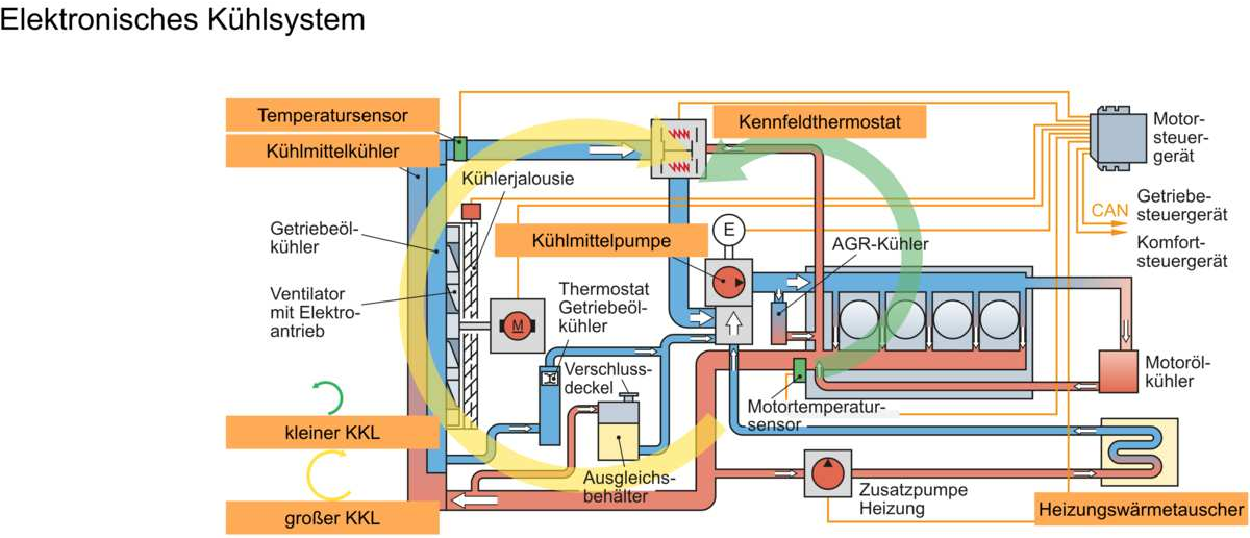
\includegraphics[width=0.7\textwidth]{images/Kuehlsystem/Kuehlsystem-1.pdf}
\caption{Kennfeldkühlung, Quelle: Europa-Verlag}
%\label{fig:}%% anpassen
\end{figure}

zwei Betriebszustände

\begin{enumerate}
\item
  \textbf{Eco-Betrieb - Teillast} (kleiner Kühlkreislauf)

  \begin{itemize}
  \item
    Thermostatheizung: aus
  \item
    Temperatur: bis $106^\circ\text{C}$
  \item
    Warum ist der Motorwirkungsgrad höher?

    \begin{itemize}
    \item
      $\to$ der thermische Wirkungsgrad steigt aufgrund der höheren
      Motortemperatur.
    \end{itemize}
  \end{itemize}
\item
  \textbf{Volllast-Betrieb} (großer Kühlkreislauf)

  \begin{itemize}
  \item
    Thermostatheizung: an
  \item
    Temperatur: $> 90^\circ\text{C}$
  \item
    Wodurch wird ein höherer Füllungsgrad erzielt?

    \begin{itemize}
    \item
      $\to$ kältere Luft hat eine größere Dichte. Die angesaugte
      Luftmasse steigt.
    \end{itemize}
  \item
    Schutz vor Überhitzung der Motorbauteile
  \end{itemize}
\end{enumerate}

\textbf{Ansteuerung Kennfeldthermostat}, die Heizung des Thermostats
wird vom Motorsteuergerät über ein PWM-Signal angesteuert. In
Abhängigkeit von der Pulsweite und Zeit ergibt sich eine
unterschiedliche Aufheizung.

Im Dehnstoffelement ist ein Heizwiderstand eingebettet. Wenn dieser
bestromt wird, erwärmt er das Dehnstoffelement zusätzlich und die
Verstellung erfolgt nun nicht mehr allein in Abhängigkeit von der
Kühlmitteltemperatur, sondern wird vom Motorsteuergerät (nach Kennfeld,
Sollwert) vorgegeben.

\textbf{Wodurch öffnet der Kennfeldthermostat den großen Kühlkreislauf?}

\begin{enumerate}
\item
  \textbf{Eco-Modus}, das Dehnstoffelement wird vom Kühlmittel erwärmt
  und dehnt sich aus. Öffnet erst bei höheren Temperaturen
  $> 106^\circ\text{C}$.
\item
  \textbf{Volllast - Modus}, der Kennfeldthermostat wird über die
  Heizwendel erwärmt. Öffnet schon bei niedrigerer Temperatur
  $> 90^\circ\text{C}$.
\end{enumerate}

\begin{figure}[!ht]% hier: !ht
\centering
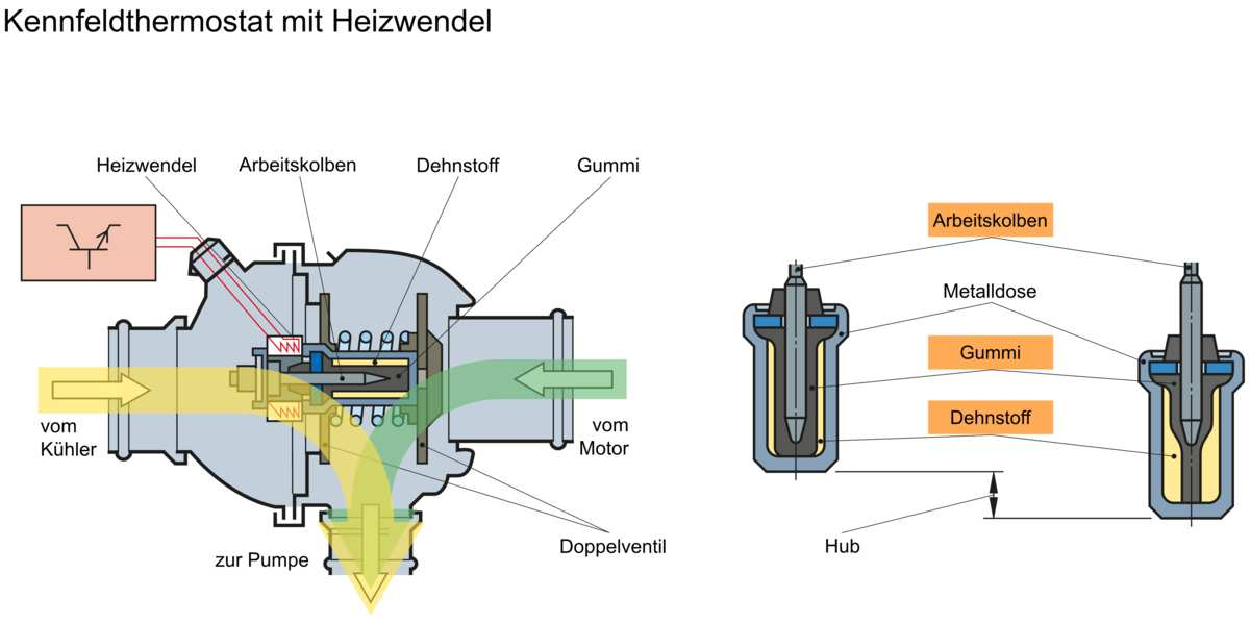
\includegraphics[width=0.6\textwidth]{images/Kuehlsystem/Kuehlsystem-2.pdf}
\caption{Kennfeldthermostat mit Heizwendel, Quelle: Europa-Verlag}
%\label{fig:}%% anpassen
\end{figure}

\newpage

\textbf{Nenne Vorteile der Kennfeldkühlung}

\begin{itemize}
\item
  schnelles Erreichen der Motorbetriebstemperatur und Katalysators
  (Begründung: vgl. Kühlmitteltemperatur bei Teillast)
\item
  Verbesserung der Innenraumheizung
\item
  Motortemperatur / Kühlmitteltemperatur bei Teillast auf bis zu
  $120^\circ\text{C}$ anheben $\to$ bis an die Grenzen der
  Zündfähigkeit

  \begin{itemize}
  \item
    verbesserte Viskosität des Motoröls $\to$ verminderte
    Motorinnenreibung
  \item
    verbesserte Gemischbildung $\to$ durch bessere Verdampfung des
    Kraftstoffs
  \item
    Verbrauchsreduzierung und die Reduzierung der Schadstoffemissionen
  \end{itemize}
\item
  Motortemperatur / Kühlmitteltemperatur bei Volllast senken $\to$
  Schutz vor Überhitzung der Motorbauteile
\end{itemize}

\textbf{Nenne Vorteile einer elektrischen Kühlmittelpumpe}

\begin{enumerate}
\item
  Förderleistung ist unabhängig von der Motordrehzahl
\item
  Pumpe kann zur schnelleren Aufheizung abgeschaltet werden
\item
  Nach Abschalten des Verbrennungsmotors kann die Pumpe weiterlaufen
\item
  Kraftstoff einsparen
\end{enumerate}

\newpage

\section{Antriebsarten von Ventilatoren /
Lüfter}\label{antriebsarten-von-ventilatoren-luefter}

\begin{enumerate}
\item
  \textbf{hydrostatischer Lüfter}
\item
  \textbf{elektrischer Lüfter}
\item
  \textbf{Lüfter mit Viscokupplung} (temperaturabhängige Kupplung,
  Riementrieb)

  \begin{enumerate}
  \def\labelenumii{\arabic{enumii}.}
  \item
    \emph{Kalter Motor}

    \begin{itemize}
    \item
      Bimetallelement verschließt Ventilöffnung
    \item
      Silikonöl wird vom Arbeitsraum in den Vorratsraum gefördert
    \item
      Antriebsscheibe hat keine Verbindung zur Lüfternabe
    \item
      Lüfter ist getrennt
    \end{itemize}
  \item
    \emph{Heißer Motor}

    \begin{itemize}
    \item
      Bimetallelement heizt sich auf und öffnet Ventilöffnung
    \item
      Silikonöl füllt sich in beiden Räumen gleich
    \item
      Kraftfluss wird stufenlos hergestellt zwischen Antriebsscheibe und
      Lüfternabe (zunehmende Reibung des Silikonöls)
    \end{itemize}
  \end{enumerate}

  \begin{itemize}
  \item
    Kühlerabluft trifft auf ein Bimetall, dessen thermische Verformung
    ein Öffnen und Schließen eines Ventils bewirkt. Abhängig von dieser
    Ventilstellung erfolgt die Einstellung der Lüfterdrehzahlen.
  \item
    \emph{Bemerkung:} System arbeitet immer mit Schlupf
    (Flüssigkeits-Haftungsbereich, Drehzahldifferenz), Antriebsscheibe
    dreht mit Riemendrehzahl, Lüfter mit Viscokupplung: nicht legen.
  \end{itemize}
\end{enumerate}

\begin{figure}[!ht]% hier: !ht
\centering
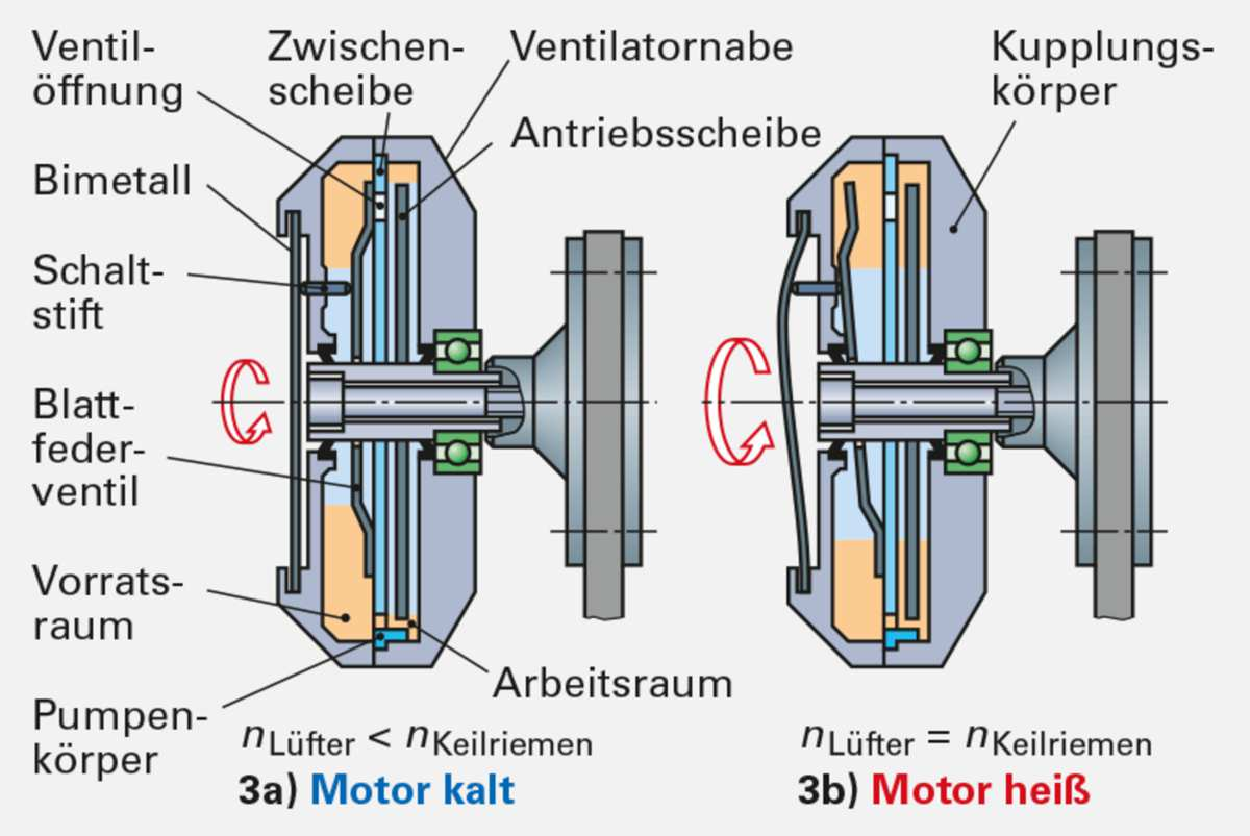
\includegraphics[width=0.5\textwidth]{images/Kuehlsystem/Kuehlsystem-3.pdf}
\caption{Viscokupplung, Quelle: Europa-Verlag}
%\label{fig:}%% anpassen
\end{figure}

\textbf{Aufgabe von Ventilatoren} bei einer bestimmten
Kühlmitteltemperatur eine ausreichende Kühlluftmenge zur Verfügung
stellen, wenn Fahrtwind nicht ausreicht bei Stillstand oder langsame
Fahrt oder Stop-and-Go-Betrieb im Stadtverkehr.

\section{Einfüllverschluss Kühlsystem
(Prüfung)}\label{einfuellverschluss-kuehlsystem-pruefung}

\begin{enumerate}
\item
  \textbf{Überdruckventil} durch den Überdruck kann die
  Kühlmitteltemperatur bis auf $120^\circ\text{C}$ ansteigen, ohne
  dass die Kühlflüssigkeit siedet.
\item
  \textbf{Unterdruckventil} beim Abkühlen der Kühlflüssigkeit tritt
  durch die Volumenverkleinerung ein Unterdruck auf. Durch das öffnende
  Ventil kann der Druck ausgeglichen werden. Dadurch wird verhindert,
  dass sich der Kühler einbeult oder Schläuche zusammenziehen.
\end{enumerate}

\begin{figure}[!ht]% hier: !ht
\centering
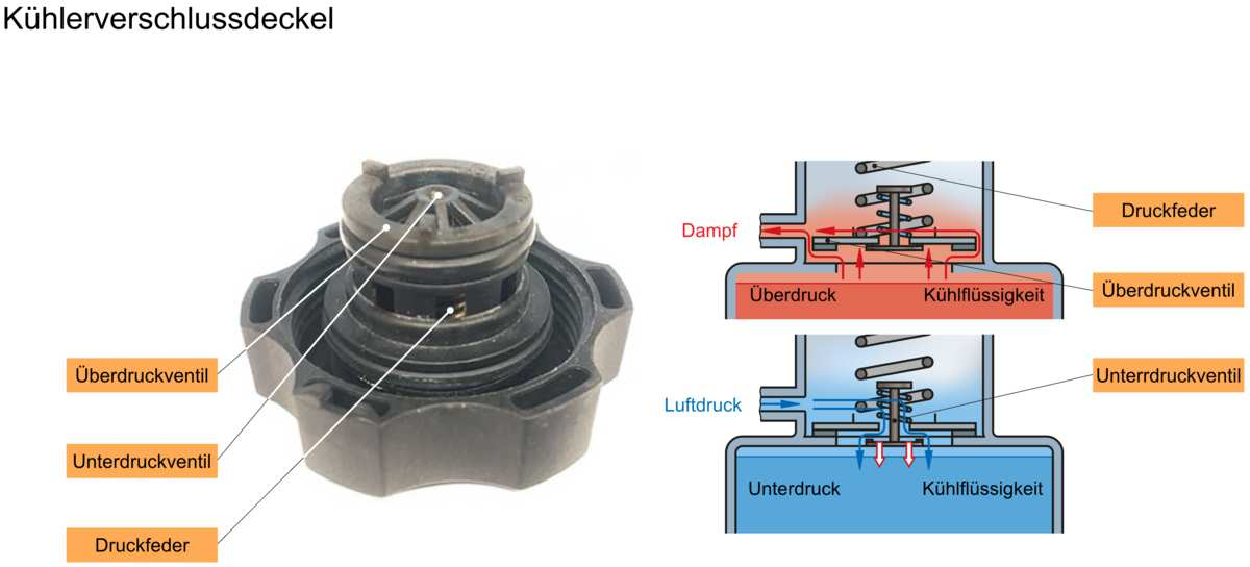
\includegraphics[width=0.7\textwidth]{images/Kuehlsystem/Kuehlsystem-4.pdf}
\caption{Kühlerverschlussdeckel, Quelle: Europa-Verlag}
%\label{fig:}%% anpassen
\end{figure}

\section{Welche Ursachen können zur Überhitzung des Motors führen?
(Motor / Kühlmittel zu
heiß)}\label{welche-ursachen-koennen-zur-ueberhitzung-des-motors-fuehren-motor-kuehlmittel-zu-heiss}

\begin{enumerate}
\item
  Lüftermotor oder Steuerung defekt
\item
  zu wenig Flüssigkeit im System (Kühlmittelverlust)
\item
  Kühllamellen verschmutzt
\item
  Kühler verstopft
\item
  Thermostat öffnet nicht
\item
  Luft im System
\item
  Überdruckventil undicht
\item
  Pumpe defekt
\item
  defekter Keilriemen
\item
  Kennfeldthermostat (Elektrische Anschluss)

  \begin{itemize}
  \item
    Leitungsbruch
  \item
    Übergangswiderstand (korrodierten Stecker) $\to$ Thermostat nicht
    richtig beheizt wird und schnell genug öffnet
  \end{itemize}
\end{enumerate}

\section{Prüfungshinweise zum
Kühlsystem}\label{pruefungshinweise-zum-kuehlsystem}

\begin{enumerate}
\item
  \textbf{Refraktometer}

  \begin{itemize}
  \item
    Dichte Batteriesäure
  \item
    Gefrierpunkt von Kühlmittel

    \begin{itemize}
    \item
      Ethylenglykolbasis G11/12
    \item
      Propylenglykolbasis G13
    \end{itemize}
  \item
    Gefrierpunkt von Scheibenwaschflüssigkeit
  \item
    Harnstoffkonzentration von AdBlue
  \end{itemize}
\item
  \textbf{Dichtheitsprüfung}

  \begin{itemize}
  \item
    Dauer: 2 Minuten
  \item
    Überdruck
  \end{itemize}
\item
  \textbf{$CO_2$-Testgerät}

  \begin{itemize}
  \item
    Undichtigkeiten zwischen Verbrennungsraum und Kühlsystem erkennen
  \end{itemize}
\end{enumerate}

Kühlmittel \emph{nicht} mischen!

\chapter{10-Loesung-Kuehlsystem}
%%ju 26-Dez-22 10-Loesung-Kuehlsystem.tex
\textbf{1. Beschreiben Sie das Funktionsprinzip der
Thermosiphonkühlung.}

\begin{itemize}
\item
  \emph{physikalische Prinzip} wärmeres, leichteres Wasser (geringe
  Dichte) steigt nach oben und kälteres, schwereres Wasser (höhere
  Dichte) sinkt nach unten.
\item
  Anwendung: Motor abstellen, dann kommt es zum Kühlmittelfluss ohne
  Pumpe
\end{itemize}

Die Umwälzung des Kühlmittels erfolgt bei der Thermosiphon bzw.
Wärmeumlaufkühlung durch die temperaturbedingte Dichteänderung des
Kühlmittels.

Erwärmt der Motor das Kühlmittel, sinkt dessen Dichte und steigt
leichter als das übrige Kühlmittel nach oben in den Kühler.

Hier nimmt die Dichte des Kühlmittels wieder zu. Fällt nach unten und
wird dem Motor von unten wieder zugeführt.

\textbf{2. Warum gibt es bei der Zwangsumlaufkühlung zwei verschiedene
Kühlkreisläufe?}

Um ein schnelles Erreichen der Betriebstemperatur zu gewährleisten.

In der Warmlaufphase soll die Temperatur mithilfe des kleinen
Kühlkreislaufs bestmöglich im Motor gehalten und verteilt werden.

Hat der Motor Betriebstemperatur erreicht, wird überschüssige Wärme über
den großen Kühlkreislauf an die Umgebung abgegeben. Das dynamische Zu-
und Abschalten des großen Kreislaufes erfolgt in der Regel mittels eines
Dehnstoffthermostates.

\textbf{3. Beschreiben Sie stichwortartig Aufbau und Funktion des
elektronischen Thermostats.}

Das elektronische Thermostat oder auch kennfeldgeregeltes Thermostat
besteht aus einem Ventil und einem Dehnstoffelement, welches mittels
einer PTC-Heizung zusätzlich erwärmt werden kann.

Es wird eingesetzt, um die Motortemperatur höher als sonst üblich
ansteigen lassen zu können. Hierdurch würde der Kraftstoffverbrauch und
der Ausstoß von HC, CO, $CO_2$, PM reduziert.

Sollte hierdurch der $NO_x$ - Ausstoß zu stark ansteigen, kann das
Steuergerät das Dehnstoffelement beheizen und hierdurch die
Motortemperatur absenken.

Um den Motor auch bei Ausfall der Elektronik vor schädlichen
Übertemperatur zu schützen, öffnet das Dehnstoffelement bei ca.
$110^\circ\text{C}$ selbsttätig.

(Bemerkung: Zündfähiges homogen-mager-Gemisch, kurz über Zündgrenze, PTC
ist selbstregelnd)

\textbf{4. Nennen Sie Ursachen und Wirkungen von Kavitation.}

Zur Kavitation kommt es bei starken Druckgefällen in einem
Hydrauliksystem. Diese können zum einen durch das strömende Medium
(Strömungskavitation) und zum anderen durch schwingende Bauteile
(Schwingungskavitation) entstehen.

Kavitation mindert zunächst den Wirkungsgrad. Infolge von Kavitation
kommt es zu einer Materialverdichtung, die bei anhaltender Kavitation zu
einem Ausbruch von Material führt.

Dieses wiederum kann im System zu Erosionsschäden führen.

\textbf{5. Wie funktioniert ein Lüfterantrieb mit Visco -- Kupplung?}

Im kalten Zustand dreht sich ein Kupplungskörper um eine
Antriebsscheibe. Ein Pumpenkörper fördert Silikonflüssigkeit aus dem
Arbeitsraum in einen Vorratsraum, aus dem sie nicht mehr entweichen
kann.

Hat die Kupplung ihre vordefinierte Einschalttemperatur erreicht, so
öffnet ein Bimetallstreifen mittels eines Schaltstiftes das
Blattfederventil, welches den Zulauf zum Arbeitsraum freigibt.

Die Silikonflüssigkeit tritt in den Arbeitsraum und verbindet die
Antriebsscheibe mit dem Pumpenkörper und der Zwischenscheibe.

Der Lüfter dreht sich. Die Silikonflüssigkeit fließt kontinuierlich von
Arbeitsraum in einen Vorratsraum und über das Ventil zurück.

Nach dem Abschalten des Lüfters durch den Bimetallstreifen wird die
Silikonflüssigkeit in den Vorratsraum zurück gefördert, kann aus diesen
aber nicht mehr entweichen. Die Lüfterkupplung trennt.

\textbf{6. Worin liegen die Vorteile eines elektrischen Lüfterantriebs?}
(Prüfung)

\begin{itemize}
\item
  Gestufte oder stufenlose Drehzahlanpassung möglich
\item
  Lüfter kann auch bei abgestelltem Motor betrieben werden

  \begin{itemize}
  \item
    Vermeidung von Hitzestau
  \end{itemize}
\item
  Kühler kann unabhängig von der Lage des Motors eingebaut werden
\item
  Antriebsmoment wird nicht von der Kurbelwelle abgezweigt

  \begin{itemize}
  \item
    hierdurch haben wir eine höhere nutzbare Antriebsleistung
  \item
    Geringeren Kraftstoffverbrauch
  \item
    Geringerer Schadstoffausstoß
  \end{itemize}
\end{itemize}

\textbf{7. Was ist ein hydrostatischer Lüfterantrieb? Wo wird ein
hydrostatischer Lüfterantrieb i.d.R. eingesetzt?}

\begin{itemize}
\item
  Anwendung: Kommt in modernen Omnibusbereichen zum Einsatz (bei
  Fahrzeugen, die keinen Fahrtwind ausgesetzt sind).
\end{itemize}

Bei einem hydrostatischen Lüfterantrieb wird mittels einer vom Motor
angetrieben Hydraulikpumpe Öldruck erzeugt, welche zum Antrieb eines
Hydrokonstantmotors eingesetzt wird und an dessen Welle sich wiederum
der eigentliche Lüfter befindet. Die Regelung erfolgt in der Regel
mittels Öldrucksteuerung.

\chapter{11-Abgasnachbehandlung}
%%ju 31-Dez-22 11-Abgasnachbehandlung.tex
\textbf{Zusammenhang von Ruß und Stickoxide}

\begin{enumerate}
\item
  \textbf{Ruß} Volllast, kalter Motor, >>Luftmangel<<, hohe
  Kraftstoffmenge (Gemisch: Fett $\lambda < 1$)
\item
  $\ce{\bold{NOx}}$ hohe Temperaturen, >>Luftüberschuss<<, geringe
  Kraftstoffmenge, (Gemisch: Mager $\lambda > 1$)
\end{enumerate}

\textbf{Katalysator} ist einen Stoff (Platin, Rhodium oder Palladium),
der eine chemische Reaktion auslöst bzw. beschleunigt, ohne dabei selbst
verbraucht zu werden.

\section{Partikel / Feinstaub}\label{partikel-feinstaub}

\textbf{Partikelmasse} (PM, Particulate Matter) entstehen bei der
unvollständigen Verbrennung.

\textbf{Zusammensetzung von Partikeln}

\begin{itemize}
\item
  Ruß ca. $65~\%$ (zusammengeballter Kohlenstoff)
\item
  mit angelagerten unverbrannte Kohlenwasserstoffverbindungen
  (krebserregend)
\item
  Sulfate
\item
  Schwermetalle
\end{itemize}

Rußpartikel tragen zur Feinstaubbelastung bei.

\textbf{Partikelemission} (Massenmessung g/km oder Trübungsmessung
$m^{-1}$)

\textbf{Partikelanzahl} (PN, Particle Number, Partikelanzahlmessung
1/km)

\textbf{Einfluss der Partikelgröße} (Zusammenhang zwischen Luftqualität
und Gesundheitsgefährdung)

\begin{itemize}
\item
  Durchmesser $< 10~\mu m$ (Feinstaub)

  \begin{itemize}
  \item
    Partikel-Gängigkeit Atmung
  \end{itemize}
\item
  Durchmesser $< 1~\mu m$ (Nanopartikel)

  \begin{itemize}
  \item
    Zellgängigkeit $\to$ Lungenbläschen (Alveolen) $\to$
    Blutkreislauf

    \begin{itemize}
    \item
      $\to$ Herz-Kreislaufsystem
    \item
      $\to$ Atemorgane
    \item
      $\to$ Krebserkrankungen
    \end{itemize}
  \end{itemize}
\end{itemize}

\section{Abgasemissionen von
Verbrennungsmotoren}\label{abgasemissionen-von-verbrennungsmotoren}

Quelle: TAK, 2022

\textbf{Rohemissionen beim Ottomotor} Abgaszusammensetzung bei einem Pkw
mit Ottomotor bei $\lambda \sim 1$ ohne Katalysator.

\begin{enumerate}
\item
  \textbf{Ansaugluft}

  \begin{enumerate}
  \def\labelenumii{\arabic{enumii}.}
  \item
    Sauerstoff ($\ce{O2}$) $\sim 21~\%$
  \item
    Stickstoff ($\ce{N2}$) $\sim 78~\%$
  \item
    Rest-/Edelgase $\sim 1~\%$
  \end{enumerate}
\item
  \textbf{Ottokraftstoff}

  \begin{enumerate}
  \def\labelenumii{\arabic{enumii}.}
  \item
    Kohlenstoff ($\ce{C}$) $\sim 84~\%$
  \item
    Wasserstoff ($\ce{H2}$) $\sim 16~\%$
  \end{enumerate}
\item
  \textbf{Nichtschadstoffe im Abgas}

  \begin{enumerate}
  \def\labelenumii{\arabic{enumii}.}
  \item
    Stickstoff ($\ce{N2}$) $\sim 71,0~\%$
  \item
    Kohlendioxid ($\ce{CO2}$) $\sim 18,0~\%$
  \item
    Wasserdampf ($\ce{H2O}$) $\sim 8,9~\%$
  \item
    Sauerstoff ($\ce{O2}$) $\sim 1,0~\%$
  \item
    Schadstoffe $\sim 1,1~\%$
  \end{enumerate}
\item
  \textbf{Schadstoffe} $\sim 1,1~\%$

  \begin{enumerate}
  \def\labelenumii{\arabic{enumii}.}
  \item
    Kohlenmonoxid ($\ce{CO}$) $\sim 0,9~\%$
  \item
    Kohlenwasserstoff ($\ce{HC}$) $\sim 0,08~\%$
  \item
    Stickoxid ($\ce{NOx}$) $\sim 0,12~\%$
  \end{enumerate}
\end{enumerate}

\textbf{Rohemissionen beim Dieselmotor} Abgaszusammensetzung bei einem
Pkw mit Dieselmotor bei $\lambda \sim 3$ ohne Katalysator.

\begin{enumerate}
\item
  \textbf{Ansaugluft}

  \begin{enumerate}
  \def\labelenumii{\arabic{enumii}.}
  \item
    Sauerstoff ($\ce{O2}$) $\sim 21~\%$
  \item
    Stickstoff ($\ce{N2}$) $\sim 78~\%$
  \item
    Rest-/Edelgase $\sim 1~\%$
  \end{enumerate}
\item
  \textbf{Dieselkraftstoff}

  \begin{enumerate}
  \def\labelenumii{\arabic{enumii}.}
  \item
    Kohlenstoff ($\ce{C}$) $\sim 86~\%$
  \item
    Wasserstoff ($\ce{H2}$) $\sim 14~\%$
  \end{enumerate}
\item
  \textbf{Nichtschadstoffe im Abgas}

  \begin{enumerate}
  \def\labelenumii{\arabic{enumii}.}
  \item
    Stickstoff ($\ce{N2}$) $\sim 76,0~\%$
  \item
    Kohlendioxid ($\ce{CO2}$) $\sim 7,0~\%$
  \item
    Wasserdampf ($\ce{H2O}$) $\sim 7,0~\%$
  \item
    Sauerstoff ($\ce{O2}$) $\sim 9,7~\%$
  \item
    Schadstoffe $\sim 0,3~\%$
  \end{enumerate}
\item
  \textbf{Schadstoffe} $\sim 0,3~\%$

  \begin{enumerate}
  \def\labelenumii{\arabic{enumii}.}
  \item
    Kohlenmonoxid ($\ce{CO}$) $\sim 0,05~\%$
  \item
    Kohlenwasserstoff ($\ce{HC}$) $\sim 0,03~\%$
  \item
    Partikel ($\ce{PM}$) $\sim 0,05~\%$
  \item
    Stickoxid ($\ce{NOx}$) $\sim 0,15~\%$
  \item
    Schwefeldioxid ($\ce{SO2}$) $\sim 0,02~\%$
  \end{enumerate}
\end{enumerate}

\textbf{Welche Auswirkungen haben Abgasemissionen auf den Menschen?}

\begin{enumerate}
\item
  $\ce{CO}$ schwerer als Luft (Vorsicht: Grube, ohnmächtig, führt zur
  Erstickung), giftig, geruchs- und farblos
\item
  $\ce{HC}$ krebserregend
\item
  $\ce{NOx}$ Reizen die Atemwege und tragen als Katalysator zu
  sommerlichen Ozonbildung bei.
\end{enumerate}

\textbf{Übersäuerung der Meere} Säure ist nicht gut für Kalk

\textbf{Wann entstehen die Schadstoffe?}

\begin{enumerate}
\item
  $\ce{CO} \text{ und } \ce{HC}$ unvollständige Verbrennung,
  Sauerstoffmangel oder Zündgrenze Fett
\item
  $\ce{PM}$ lokaler Sauerstoffmangel, Kraftstoff unter
  Sauerstoffmangel verbrannt wird
\item
  $\ce{NOx}$ hohe Verbrennungsdrücke und Verbrennungstemperaturen
\item
  $\ce{SO2}$ Bestandteil des Kraftstoffs
\end{enumerate}

\textbf{Unvollständige Verbrennung} $\ce{HC}, \ce{CO}$, Partikel und
Ruß (Sauerstoffmangel)

\textbf{Light-off-point} (Prüfung) beschreibt das Temperaturniveau (ca.
$350^\circ\text{C}$) bei dem eine Abgaskonvertierung von ca. 50 \%
stattfindet (Schadstoffumwandlung, Zusammenhang von
Katalysatortemperatur und Konvertierungsgrad).

\section{Schadstoffreduzierung oder
Minderung}\label{schadstoffreduzierung-oder-minderung}

\begin{enumerate}
\item
  \textbf{Außermotorisch} (Bauteile können getauscht werden)

  \begin{enumerate}
  \def\labelenumii{\arabic{enumii}.}
  \item
    Katalysator (Oxydationskatalysator bis 90 \% Konvertierungsrate in
    nicht Schadstoffe)
  \item
    Sekundärluftsystem (Luft in den Abgaskrümmer einblasen,
    Nachverbrennen der Abgase, Abgastemperatur erhöhen, schnell
    Light-off-Point erreichen)
  \item
    DPF
  \item
    SCR-Kat ($\ce{NOx}$ reduzieren)
  \item
    $\ce{NOx}$-Speicherkatalysator
  \item
    DPNR (Toyota, Diesel Particulate - NOx Reduction System, Rußpartikel
    und Stickoxid)
  \end{enumerate}
\item
  \textbf{Innermotorisch}

  \begin{enumerate}
  \def\labelenumii{\arabic{enumii}.}
  \item
    AGR (Hochdruck, Niederdruck)
  \item
    Brennraumoptimierung (Kolbenform: Muldenkolben oder Kompressionsraum
    $\to$ bessere Vermischung, bessere Verdunstung des Kraftstoffs,
    vollständigeren Verbrennung, weniger Ruß)
  \item
    Mehrventiltechnik (Liefergrad, Füllungsgrad bedarfsgerecht)
  \item
    Erhöhung der Einspritzdrücke
  \item
    Ladedruckregelung und Ladeluftkühlung
  \item
    Verfeinerung des Strahlbildes (Injektor)
  \item
    Optimierung von Einspritzbeginn und Menge (über Druck und Zeit,
    Mehrfacheinspritzung)
  \item
    Glühzeitsteuerung
  \item
    Einlasskanalsteuerung / Einlasskanalabschaltung (vollständigeren
    Verbrennung, Drallkanal, Füllungskanal mit Klappe, niedriger Last
    und Drehzahl vs.~steigender Motordrehzahl bzw. -last)
  \item
    Temperaturmanagement (höhere Betriebstemperatur der Motoren, weniger
    Kraftstoff notwendig)
  \end{enumerate}
\end{enumerate}

\section{Leitgrößen in der Abgasuntersuchung
(AU)}\label{leitgroessen-in-der-abgasuntersuchung-au}

\begin{enumerate}
\item
  $\ce{HC}$
\item
  $\ce{CO}$
\item
  $\ce{CO2}$
\item
  $\ce{O2}$
\item
  Leerlaufdrehzahl
\item
  Viergasmessung
\item
  Plakettenwert, Trübungswert (k-Wert)
\item
  Rauchgastrübungsmessung (Trübung des Abgases, Rauchbildung)
\item
  Partikelanzahlmessung (Diesel ab EURO 6, ersetzt
  Rauchgastrübungsmessung)
\item
  Motorkontrollleuchte (MIL) und Kontrollleuchte für den Partikelfilter
  muss nach Motorstart erloschen sein. Ist dies nicht der Fall, gilt die
  AU als nicht bestanden.
\item
  \textbf{RDE-Test} (Real Driving Emissions, dt.: reales Abgasverhalten,
  die Schadstoffemissionen $\ce{NOx, Partikel, CO, HC}$ werden auf der
  Straße ermittelt)
\end{enumerate}

\section{Herkunft der Kraftstoffe und ihre Nutzung in
Antrieben}\label{herkunft-der-kraftstoffe-und-ihre-nutzung-in-antrieben}

\begin{enumerate}
\item
  \textbf{Primärenergieträger}

  \begin{enumerate}
  \def\labelenumii{\arabic{enumii}.}
  \item
    Fossile Energieträger

    \begin{itemize}
    \item
      Erdöl, Kohle, Uran, Erdgas $\to$ Wasserstoff
    \end{itemize}
  \item
    Regenerative Energieträger

    \begin{itemize}
    \item
      Wind, Wasser, Solar, Biomasse $\to$ Bio-Diesel, Bio-Ethanol
    \end{itemize}
  \end{enumerate}
\item
  \textbf{Nutzenergieträger}

  \begin{enumerate}
  \def\labelenumii{\arabic{enumii}.}
  \item
    Kraftstoffe

    \begin{itemize}
    \item
      Benzin, Diesel, Erdgas (CNG), Autogas (LNG) $\to$
      Verbrennungsmotor
    \end{itemize}
  \item
    Elektrische Energie $\to$ Batterie
  \item
    Wasserstoff $\to$ Brennstoffzelle oder Verbrennungsmotor
  \end{enumerate}
\item
  \textbf{Antrieb}

  \begin{enumerate}
  \def\labelenumii{\arabic{enumii}.}
  \item
    Verbrennungsmotor
  \item
    E--Motor (Brennstoffzelle oder Batterie)
  \item
    Hybrid (Verbrennungsmotor und E--Motor)
  \end{enumerate}
\end{enumerate}

\section{Abgasrückführung (AGR)}\label{abgasrueckfuehrung-agr}

\textbf{Abgasrückführung,} Maßnahme zur Verminderung des
Stickoxidausstoßes.

Abgas wird aus dem Auspuff entnommen $\to$ über Abgaskühler abgekühlt
und über ein AGR-Ventil in das Saugrohr geleitet $\to$ vermischt mit
Frischluft und dem Brennraum wieder zugeführt. Alternative, eine
übergroße Ventilüberschneidung.

Die Abgase vermindern die angesaugte Frischluftmenge und senken die
Verbrennungstemperaturen. Zudem wirken die nicht brennbaren Gase kühlend
(Abgastemperatur $<1000^\circ\text{C} \iff$ Verbrennungstemperatur
$\le2500^\circ\text{C}$). NOx-Ausstoß sinkt.

\begin{itemize}
\item
  weniger Sauerstoff $\to$ geringere Kraftstoffmenge (homogen)
\item
  Verbrennungsdruck und Verbrennungstemperatur verringern sich
\item
  $\ce{NOx}$ sinkt
\end{itemize}

Bei hohen Drehzahlen und Volllast wird AGR abgeschaltet, sonst steigen
die Rußpartikel durch Frischluftmangel.

\textbf{Wodurch entstehen $\ce{\bold{NOx}}$?}

\begin{enumerate}
\item
  hohe Brennraumtemperaturen und Verbrennungsdrücke
\item
  hohe Flammgeschwindigkeiten bei Sauerstoffüberschuss
\end{enumerate}

\textbf{AGR-Rate} bis zu 60 \% bei Teillast und niedrige Last (80 Km/h
Landstraße, Pkw-Direkteinspritzern)

\textbf{Varianten der Abgasrückführung}

\begin{enumerate}
\item
  \textbf{interner AGR}

  \begin{itemize}
  \item
    über die Ventilsteuerzeiten wird die zurückgeführte Abgasmenge
    beeinflusst
  \item
    \emph{Nachteil:} hohe Temperaturen der Abgase begrenzt die mögliche
    AGR-Rate
  \end{itemize}
\item
  \textbf{externer AGR}

  \begin{enumerate}
  \def\labelenumii{\arabic{enumii}.}
  \item
    \textbf{Hochdruck-AGR}

    \begin{itemize}
    \item
      \emph{Entnahmestelle:} das Abgas wird vor dem >>Turbolader<<
      entnommen und über das AGR-Ventil dem Saugrohr zugeführt
    \item
      \emph{Nachteil:} heißes, unbereinigtes Abgas, voller Rußgehalt
    \item
      \emph{Vorteil:} Warmlaufphase verkürzen, Katalysator schnell auf
      Betriebstemperatur bringen
    \end{itemize}
  \item
    \textbf{Niederdruck-AGR}

    \begin{itemize}
    \item
      \emph{Entnahmestelle:} das Abgas wird hinter dem
      >>Oxydationskatalysator/DPF<< entnommen, über den AGR-Kühler und
      AGR-Ventil vor dem Verdichterrad des Turboladers die Frischluft
      wieder zugeführt.
    \item
      \emph{Vorteile:}

      \begin{enumerate}
      \def\labelenumiii{\arabic{enumiii}.}
      \item
        das zurückgeführte Abgas ist gereinigt und gekühlt
        (Verdichterrad)
      \item
        dem Turbolader steht die volle Abgasenergie zur Verfügung
        (Ansprechverhalten)
      \item
        gute Vermischung von Frischluft und Abgas (Gleichverteilung,
        höhere AGR-Raten)
      \end{enumerate}
    \item
      \emph{Nachteil:} größerer Bauaufwand
    \end{itemize}
  \end{enumerate}
\end{enumerate}

\section{Sekundärluftsysteme}\label{sekundaerluftsysteme}

Schnelles Aufheizen der Abgasnachbehandlungssysteme durch Erhöhen der
Abgastemperatur. Das Einbringen von Frischluft in den Abgaskrümmer
unmittelbar hinter die Auslassventile führt zu einer Nachverbrennung der
heißen Abgase.

\begin{itemize}
\item
  \textbf{Sekundärluft} wird über eine \textbf{elektrische
  Sekundärluftpumpe} und ein \textbf{Sekundärluftventil} in das
  Abgas-System eingeblasen.
\item
  \textbf{Rückschlagventil} verhindert ein Zurückströmen heißer Abgase.
\item
  \textbf{Motorsteuergerät} steuert Sekundärluftpumpe und
  Sekundärluftventil zeitgleich an.
\end{itemize}

\section{3-Wege-Katalysator (Ottomotor mit
Saugrohreinspritzung)}\label{wege-katalysator-ottomotor-mit-saugrohreinspritzung}

\textbf{Aufbau}

\begin{itemize}
\item
  Keramikträger oder Edelstahlträger (hohe Hitzebeständigkeit, erreicht
  schnelle Betriebstemperatur)
\item
  Durch das Aufbringen einer Zwischenschicht aus Aluminiumoxid
  vergrößert sich die Grundfläche des Trägers. Auf diese Fläche wird der
  eigentliche Katalysator aufgedampft.
\item
  \emph{Edelmetalle:} Platin, Palladium, Rhodium
\item
  Ottomotor: wird im Lambdafenster von $0,997 <\lambda< 1,004$
  betrieben
\item
  Magermix-Motoren: $\lambda>1,004$ nimmt die Reduktion von
  Stickoxiden aufgrund des Sauerstoffüberschusses ab
  (NOx-Speicherkatalysator notwendig)
\end{itemize}

\textbf{Funktion}

\begin{itemize}
\item
  \textbf{Chemische Prozesse}

  \begin{enumerate}
  \item
    Reduktion $\ce{NOx} \to \ce{N2 + O2}$
  \item
    Oxidation $\ce{CO} \to \ce{CO2}$
  \item
    Oxidation $\ce{HC} \to \ce{CO2 + H2O}$
  \end{enumerate}
\item
  \textbf{Betriebstemperatur} ca. $400 - 800^\circ\text{C}$

  \begin{itemize}
  \item
    fördert und beeinflusst die Oxidation- und Reduktionsvorgänge
  \end{itemize}
\item
  \textbf{Konvertierungsrate} bis zu $90~\%$
  (Schadstoffumwandlungsrate, Verbrennung des Kraftstoff-Luftgemisches
  bei $\lambda = 1$, stöchiometrisch $\hat{=}$ Lambda 1)
\item
  \textbf{Mindesttemperatur} ca. $350^\circ\text{C}$
\item
  thermischen Alterung ca. $> 900^\circ\text{C}$
\item
  Zerstörung des Katalysators ca. $>1000^\circ\text{C}$
\item
  \textbf{Einbauposition des Katalysators,} motornahe Einbauposition,
  dadurch bekommt er heißere Abgase und erreicht somit schneller seine
  Betriebstemperatur. Risiko einer Überhitzung des Katalysators bei
  hoher Motorlast bzw. Drehzahl.
\end{itemize}

\section{Oxydationskatalysator}\label{oxydationskatalysator}

\textbf{Aufbau}

Keramikträger oder Edelstahlträger, Zwischenschicht (Wash Coat)

Auf dem Keramikträger ist zur Vergrößerung der wirksamen Oberfläche eine
Beschichtung aus Aluminiumoxid aufgebracht. Auf der Trägerschicht
befindet sich der eigentliche Katalysator (Platin).

\textbf{Funktion}

\begin{itemize}
\item
  Oxidieren $\hat{=}$ Verbrennen
\item
  \textbf{Chemische Prozesse}

  \begin{enumerate}
  \item
    $\ce{CO} \to \ce{CO2}$
  \item
    $\ce{HC} \to \ce{CO2 + H2O}$
  \item
    $\ce{NO1} \to \ce{NO2}$ (Stickstoffmonoxid $\to$
    Stickstoffdioxid, Fahrzeuge mit Partikelfilter)

    \begin{itemize}
    \item
      $\ce{NO2}$ senkt die Zündtemperatur von Rußpartikeln auf ca.
      $300 - 450^\circ\text{C}$ und fördert die Regeneration von
      Rußpartikel (Beispiel: längerem Volllastbetrieb bei einer
      Autobahnfahrt)
    \item
      $\ce{NO/NO2}$-Verhältnis (vgl. SCR-Kat.)
    \end{itemize}
  \end{enumerate}
\item
  \textbf{Temperatur} wegen des hohen Sauerstoffgehalts im Abgas setzt
  die Wirkung bei ca. $> 170^\circ\text{C}$ ein
\end{itemize}

\textbf{Warum können bei einem Oxydationskatalysator keine
$\ce{\bold{NOx}}$ reduziert werden?}

Durch den Luftüberschuss im Abgas.

Volllast: $\lambda \approx 1,3$, Leerlauf: $\lambda \approx 18$

\section{Partikelfilter (DPF Dieselpartikelfilter / OPF
Ottopartikelfilter)}\label{partikelfilter-dpf-dieselpartikelfilter-opf-ottopartikelfilter}

\textbf{Wovon ist die Bildung von Rußpartikeln abhängig?}

\begin{enumerate}
\item
  Luftzufuhr
\item
  Zerstäubung des Kraftstoffs und
\item
  Flammenausbreitung
\end{enumerate}

\textbf{Wodurch können die Partikel begrenzt werden?}

\begin{enumerate}
\item
  Kraftstoff unter hohem Druck fein zerstäubt in der richtigen Menge und
  zum günstigsten Zeitpunkt eingespritzt wird.
\item
  Kraftstoffqualität
\item
  Erhöhung der Cetanzahl (Zündwilligkeit)
\item
  Verringerung des Schwefelgehaltes
\end{enumerate}

\textbf{Vollstrom-Partikelfilter (Hauptstromfilter, geschlossenes
System, über 98 \%) vs.~Teilstrom-Partikelfilter (Nebenstromfilter, 30
-- 70 \% Partikel zurückhalten)}

Filtermaterial: Keramik, Siliziumcarbid oder Sintermetall

Im Keramikkörper sind die Kanäle wechselseitig verschlossen.

Das gesamte Abgas muss durch das poröse Keramikmaterial strömen.
Porengröße: gasförmige Abgase strömen durch und Partikel bleiben zurück.

\textbf{Erfassung des Beladungszustands}

Nimmt die Beladung weiter zu, erhöht sich der Abgasgegendruck des
Filters. Der Differenzdrucksensor misst den Druckunterschied vor und
nach dem Partikelfilter. Im SG sind Kennlinien mit Sollwerten für einen
defekten, sauberen und einen beladenen Filter abgelegt.

\begin{itemize}
\item
  Partikelmasse (PM) $\to$ Ruß (Kohlenstoff)
\item
  \textbf{Chemische Prozesse}

  \begin{itemize}
  \item
    Rußpartikel $\to \ce{CO2}$ verbrannt
  \item
    Ruß kann bei Temperaturen von ca. $550^\circ \text{C}$ zu
    gasförmigen Kohlendioxid verbrannt werden. Rest ist Asche.
  \item
    Additiv: Absenkung der Partikelabbrenntemperatur
  \item
    Größe: 1/1000 -- 1/100 mm
  \end{itemize}
\item
  \textbf{3x Arten der Regenerierung des DPF} Zündtemperatur von
  Rußpartikel ca. $550 - 600^\circ\text{C}$

  \begin{enumerate}
  \item
    \textbf{natürliche Regenerierung}

    \begin{itemize}
    \item
      Regenerierung erfolgt nach spätestens 1000 km
    \item
      längere Autobahnfahrt mit höherer Motorleistung erforderlich,
      Prozess läuft langsam ab
    \item
      Oxy-Kat erforderlich:

      \begin{itemize}
      \item
        $\ce{NO} \to$ $\ce{NO2}$ für Oxidation von Ruß
      \item
        Nachoxydation von $\ce{CO und HC} \to$ um Abgastemperatur
        anheben
      \end{itemize}
    \end{itemize}
  \item
    \textbf{erzwungene, aktive Regenerierung} (bei häufigem
    Kurzstreckenbetrieb)

    \begin{enumerate}
    \def\labelenumii{\arabic{enumii}.}
    \item
      \textbf{Stufe} Abgastemperatur durch eine Nacheinspritzung
      erhöhen, um den Oxydationskatalysator auf Betriebstemperatur zu
      bringen. (Motorbrenner)
    \item
      \textbf{Stufe} Nacheinspritzung erfolgt spät, sodass der
      Kraftstoff im Zylinder nur verdampft. Der gasförmige Kraftstoff
      verbrennt erst im Katalysator vor dem Partikelfilter und heizt den
      Filter auf die Zündtemperatur der Partikel auf (Katbrenner).

      \begin{itemize}
      \item
        Dauer: 5 -- 15 Min.
      \item
        Motorlast anheben: zusätzliche Verbraucher, Glühkerzen,
        Heckscheibenheizung, AGR abschalten
      \item
        \textbf{Temperaturerhöhung}

        \begin{enumerate}
        \def\labelenumiii{\arabic{enumiii}.}
        \item
          \emph{Pkw} Nacheinspritzung in den Zylinder zum Ende des
          Arbeitstaktes
        \item
          \emph{Lkw} Nacheinspritzung über einen Auspuffinjektor
          (HC-Doser) in das Auspuffrohr (verhindert eine Verdünnung des
          Motoröls)

          \begin{itemize}
          \item
            Katalysator Nachverbrennung
          \item
            Anstieg der Abgastemperatur $\to$ Ruß abbrennen $\to$
            Rest-Asche
          \end{itemize}
        \end{enumerate}
      \end{itemize}
    \end{enumerate}
  \item
    \textbf{Zwangsregenerierung} (Kfz-Werksatt, wenn Regeneration durch
    Motorstopp unterbrochen wurde)

    \begin{itemize}
    \item
      Kontrollleuchte DPF an
    \item
      Motor auf Betriebstemperatur
    \item
      mit einem Diagnosetester kann die Regeneration im Stand ausgelöst
      werden. Dabei läuft der Motor unter Aktivierung der
      Nebenverbraucher mehrere Minuten mit hohen Drehzahlen. Durch die
      hohen Abgastemperaturen sollte man keine Abgasanlage anschließen.
    \item
      Ölwechsel (Empfehlung wegen Ölverdünnung)
    \item
      Dauer: 5 -- 45 Min.
    \end{itemize}
  \end{enumerate}
\item
  \textbf{bei längerem Kurzstreckenverkehr} Abgastemperatur nur selten
  $> 250^\circ\text{C}$, findet keine oder eine unzureichende
  Regeneration statt. Partikelfilter setzt sich zu und es kommt zu einem
  erhöhten Abgasgegendruck. Kontrollleuchte für den Partikelfilter wird
  angesteuert.
\end{itemize}

\section{NOx-Speicherkatalysator zur
NOx-Minderung}\label{nox-speicherkatalysator-zur-nox-minderung}

\begin{itemize}
\item
  \textbf{Anordnung der Katalysatoren im Abgasstrang}

  \begin{itemize}
  \item
    Motor $\to$ Oxydationskatalysator (DOC, Oxidation von
    $\ce{CO und HC}$) $\to$ DPF (Rußpartikel filtern) $\to$
    $\ce{NOx}$-Speicherkatalysator ($\ce{NOx}$ speichern 50 -- 70
    \%)
  \end{itemize}
\item
  \textbf{Chemische Prozesse}

  \begin{enumerate}
  \item
    Beladungsphase $\lambda > 1$ (mager Betrieb), Dauer: 30 -- 300 s

    \begin{itemize}
    \item
      Bedingung: im Oxykat: muss $\ce{NO+O2} \to$ $\ce{NO2}$
      umgewandelt werden (wir brauchen einen hohen Anteil
      Stickstoffdioxid)
    \item
      Speichermedium Bariumoxid reagiert zusammen mit $\ce{NOx}$ zu
      Bariumnitrat
    \end{itemize}
  \item
    NOX-Speicherkatalysator regenerieren (Speicherfähigkeit erschöpft)
    $\lambda < 1$ (fetten Betrieb), Dauer: 2 -- 10 s

    \begin{itemize}
    \item
      Reduktionsmittel: unverbrannte Kohlenwasserstoffe (durch Anfetten)
      reagieren mit dem Sauerstoff von Bariumnitrat und reduzieren ihn
      zu Bariumoxid
    \end{itemize}
  \end{enumerate}
\item
  \textbf{Was ist eine Schwefelvergiftung,} Schwefel reagiert mit
  Bariumoxid zu Bariumsulfat, wodurch die Speicherfähigkeit des
  Katalysators herabgesetzt wird. Das SG erkennt durch immer kürzer
  werdenden Beladungsphasen und leitet eine Schwefelregeneration ein.
\item
  \textbf{Schwefelregeneration} (Entschwefelung, Desulfatisierung):

  \begin{itemize}
  \item
    nach etwa 5000 km frei brennen
  \item
    Durch Nacheinspritzung wird die Abgastemperatur im
    NOx-Speicherkatalysator auf etwa $> 650^\circ\text{C}$ gebracht.
    Schwefel verbrennt auf der Oberfläche.
  \end{itemize}
\item
  \textbf{Temperaturen} zwischen ca. $250 - 550^\circ\text{C}$ wird
  für eine \textbf{höchste $\ce{NOx}$-Umwandlung} benötigt
\item
  \textbf{Temperaturen} $> 750^\circ\text{C}$ \textbf{schädigen} den
  Speicherkatalysator
\end{itemize}

\section{SCR-Katalysator}\label{scr-katalysator}

\begin{itemize}
\item
  \textbf{AdBlue} hochreine, 32,5 \% - ige wässrige Harnstofflösung

  \begin{itemize}
  \item
    Ammoniakträger AdBlue, Reduktionsmittel Amoniak ($\ce{NH3}$)
  \item
    Mischungsverhältnis (Harnstoff 32,5 \%, Wasser 67,5 \%)
  \item
    Gefrierpunkt $< -11^\circ\text{C}$
  \item
    Refraktometer: Harnstoffgehalt messen
  \end{itemize}
\item
  \textbf{SCR} selective, also bevorzugte katalytische Reduktion
  (vordergründig Stickoxide verringern)
\item
  \textbf{Anordnung der Katalysatoren im Abgasstrang}

  \begin{itemize}
  \item
    Motor $\to$ Oxydationskatalysator ( = Diesel Oxidation Catalytic
    Converter, Oxidation von $\ce{CO und HC}$) $\to$ DPF
    (Rußpartikel filtern) $\to$ AdBlue eindüsung $\to$
    SCR-Katalysator ($\ce{NOx}$-Reduktion)
  \end{itemize}
\end{itemize}

\textbf{Funktion}

\begin{itemize}
\item
  Nach Eindüsung des Reduktionsmittels (AdBlue) in den Abgasstrang muss
  zunächst Ammoniak ($\ce{NH3}$) gebildet werden.
\item
  Ammoniakbildung erfolgt in zwei Phasen

  \begin{enumerate}
  \item
    \textbf{Thermolyse} Harnstoff wird durch Einfluss der Abgaswärme
    $\to$ in Ammoniak $\ce{NH3}$ und Isocyansäure umgewandelt
  \item
    \textbf{Hydrolyse} durch Einfluss von Wasser wird die unerwünschte
    Isocyansäure in $\ce{CO2}$ und Ammoniak $\ce{NH3}$ umgewandelt
  \end{enumerate}
\item
  Das entstandene Ammoniak muss im Katalysator an einer
  Speicherkomponente zwischengespeichert werden.

  \begin{itemize}
  \item
    $\ce{NH3}$-Speicherkomponente: Zeolith, Titan, Vanadium,
    Wolfram-Oxid-Verbindungen (Beschichtung)
  \end{itemize}
\item
  \textbf{Chemische Prozesse}

  \begin{itemize}
  \item
    Stickoxide ($\ce{NO und NO2}$) treffen im Katalysator auf den
    zwischen gespeicherten Ammoniak ($\ce{NH3}$) und werden in
    Stickstoff ($\ce{N2}$) und Wasserdampf ($\ce{H2O}$) umgewandelt
    und in Kohlendioxid ($\ce{CO2}$).
  \item
    Reaktion läuft bei Temperaturen $> 200^\circ\text{C}$ ab
  \item
    schnelle SCR-Reaktion

    \begin{itemize}
    \item
      ausgewogenes $\ce{NO/NO2}$-Verhältnis wird im
      Oxidationkatalysator durch Oxidation von $\ce{NO} \to \ce{NO2}$
      hergestellt
    \end{itemize}
  \end{itemize}
\item
  \textbf{Temperatur} ca. $250 - 450^\circ\text{C}$
\end{itemize}

\section{Fragen zur
Abgasnachbehandlung}\label{fragen-zur-abgasnachbehandlung}

\textbf{Motorische Notlaufmaßnahmen dienen $\ldots$}

Der Erhaltung der Fahrsicherheit, der Vermeidung von Folgeschäden und
der Minimierung von Abgasemissionen.

\textbf{Welche Gemischbildung wird bei Dieselmotoren und direkt
einspritzenden Ottomotoren eingesetzt?}

Innere Gemischbildung

\textbf{Wofür steht die Abkürzung SCR?}

Selective Catalytic Reduction

\textbf{Welche Aufgabe hat der NOx-Sensor nach dem SCR-Katalysator?}

Er dient unter anderem zur Überwachung des Wirkungsgrades des
SCR-Systems.

\textbf{Was misst der $\ce{NOx}$-Sensor?}

Die Menge an $\ce{NOx}$ messen.

\textbf{Welche Aussage ist richtig bezüglich der Reduzierung der
Abgasemissionen?}

Die Emissionsreduzierung kann zumindest teilweise durch innermotorische
Maßnahmen umgesetzt werden.

\textbf{Was versteht man unter der >>passiven Regeneration<< eines
Dieselpartikelfilters?}

Die Rußpartikel werden ohne Eingriff der Motorsteuerung kontinuierlich
verbrannt.

\begin{enumerate}
\item
  \textbf{passive Regeneration DPF} durch den täglichen Betrieb wird die
  Abgas-Regeneration eingeleitet.
\item
  \textbf{aktive Regeneration DPF} SGe Eingriff in das System

  \begin{itemize}
  \item
    Gefahr der Öl-Verdünnung, wenn Regeneration unterbrochen wird.
  \end{itemize}
\end{enumerate}

\textbf{Welche Aussage ist richtig bezüglich der Entstehung von
Rußpartikeln?}

Rußpartikel entstehen in den lokal fetten Gemischzonen des Brennraums.

\textbf{Was ist AdBlue?}

AdBlue ist ein Betriebsstoff zur Abgasnachbehandlung, der aus Harnstoff
und aus destilliertem/demineralisiertem Wasser besteht.

\textbf{Welche Aufgabe hat das Reduktionsmittel AdBlue?}

AdBlue reduziert die Stickoxidemissionen fast vollständig und senkt den
Partikelausstoß.

\textbf{Das Umkehrventil beim AdBlue-System hat die Aufgabe, das
$\ldots$}

Kein AdBlue in der Förderleitung und im Einspritzventil bei kalten
Außentemperaturen gefrieren kann.

\textbf{Durch welche der aufgeführten Stoffe werden das Verbrennen der
Rußpartikel bei der Regeneration des Dieselpartikelfilters verbessert?}

Platin

\textbf{Bei Motor fernen Dieselpartikelfiltern kommt ein
Kraftstoff-Additiv zum Einsatz. Welche Aufgabe hat dieses Additiv?}

Durch das Additiv sinkt die Verbrennungstemperatur der Rußpartikel auf
ca. $500^\circ\text{C}$, damit die Regeneration des Partikelfilters
auch bei Teillastbetrieb möglich ist.

\textbf{Welches Sensorsignal wird vom Motorsteuergerät zur Mittlung der
Rußbeladung des Partikelfilters unter anderem benötigt?}

Das Signal des Abgastemperatursensors vor dem Partikelfilter.

\textbf{Wie groß ist in etwa ein Rußpartikel, das beim
Verbrennungsprozess eines Dieselmotors entsteht?}

$0,02 - 0,05~\mu m$

\textbf{Warum ist Feinstaub gefährlicher als Rußpartikel?}

Feinstaub ist Zell gängig $\to$ Krebs

\textbf{Welche Eigenschaft hat das Reduktionsmittel AdBlue?}

Es gefriert bei einer Temperatur $\leq -11^\circ\text{C}$

\textbf{Welche Aufgabe hat die Abgasrückführung?}

Durch die Abgasrückführung werden die $\ce{NOx}$-Emissionen gesenkt.

\textbf{Welche Auswirkung hat der Betrieb mit einem vollständig
entleerten Reduktionsmittel Tank bei Pkw?}

Der Verbrennungsmotor lässt sich beim nächsten Versuch nicht mehr
starten.

\textbf{Stickoxide aus der motorischen Verbrennung schädigen $\ldots$}

Die Umwelt durch Smog und >>Sauren Regen<<.

\textbf{Eine Schaltdiode wird eingesetzt $\ldots$}

Zum schnellen Umschalten von hoher auf niedrige Impedanz und umgekehrt.

\textbf{Durch die OBD-Gesetzgebung muss $\ldots$}

Fehlerspeicherinformationen und der Zugriff auf diese Informationen
standardisiert werden.

\textbf{Bei der Desulfatisierung (Entschwefelung) wird $\ldots$}

Der $\ce{NOx}$-Speicherkatalysator zur Schwefelregenerierung für eine
bestimmte Zeit (z. B. 5 Minuten) auf über $650^\circ\text{C}$
aufgeheizt und mit fettem Abgas $\lambda < 1$ beaufschlagt.

\textbf{Aufgrund gesetzlicher Vorgaben müssen Systeme für die Erkennung
von Verbrennungsaussetzern $\ldots$}

Bei Ottomotoren in jedem Betriebspunkt und bei Dieselmotoren nur im
Leerlauf aktiv sein.

\chapter{11-Loesung-Schadstoffminderung-Diesel}
%%ju 31-Dez-22 11-Loesung-Schadstoffminderung-Diesel.tex
\textbf{1. Welches Ziel wird mit der Abgasrückführung verfolgt?}

Durch die Rückführung von nicht brennbaren Abgasen in den Zylinder wird
die Verbrennungsspitzentemperatur gesenkt, um den Ausstoß von
Stickoxiden zu reduzieren.

\textbf{2. Beschreiben Sie Aufbau und Funktion der
Einlasskanalsteuerung.}

Motoren mit einer Einlasskanalsteuerung verfügen einlassseitig über
einen Drall- und Füllungskanal.

Der Drallkanal versetzt die durchströmende Luft in Drehbewegung. Im
unteren Drehzahl und Lastbereich ist nur Drallkanal geöffnet. Die
angesaugte Luft gerät Strudel förmig in den Zylinder, wodurch es zu
einer besseren Durchmischung des eingespritzten Kraftstoffes kommt.

Um bei hohen Drehzahlen und Lasten eine ausreichende Zylinderfüllung zu
gewährleisten, wird hier der Füllungskanal durch die Füllungsklappe
freigegeben. Der hohe Luftdurchsatz im Drallkanal sorgt dafür, dass die
Luft, die ihm durchströmt, angedreht wird.

Die Luft aus dem Füllungskanal wird im Zylinder von der Luft aus dem
Drallkanal mitgerissen und gerät so ebenfalls in Drehbewegung.

\textbf{3. Welcher Teil der Abgase eines Dieselmotors gehört zu den
Schadstoffen / Nichtschadstoffen?}

\begin{enumerate}
\item
  \textbf{Nichtschadstoffe im Abgas}

  \begin{enumerate}
  \def\labelenumii{\arabic{enumii}.}
  \item
    Stickstoff ($\ce{N2}$) $\sim 76,0~\%$
  \item
    Kohlendioxid ($\ce{CO2}$) $\sim 7,0~\%$
  \item
    Wasserdampf ($\ce{H2O}$) $\sim 7,0~\%$
  \item
    Sauerstoff ($\ce{O2}$) $\sim 9,7~\%$
  \end{enumerate}
\item
  \textbf{Schadstoffe} $\sim 0,3~\%$

  \begin{enumerate}
  \def\labelenumii{\arabic{enumii}.}
  \item
    Kohlenmonoxid ($\ce{CO}$) $\sim 0,05~\%$
  \item
    Kohlenwasserstoff ($\ce{HC}$) $\sim 0,03~\%$
  \item
    Partikel ($\ce{PM}$) $\sim 0,05~\%$
  \item
    Stickoxid ($\ce{NOx}$) $\sim 0,15~\%$
  \item
    Schwefeldioxid ($\ce{SO2}$) $\sim 0,02~\%$
  \end{enumerate}
\end{enumerate}

\textbf{4. Wie werden die Stickoxide im NOx-Speicherkatalysator
gehalten?}

$\ce{NO}$ Bestandteile des Abgases werden mithilfe des vorgeschalteten
Oxidationskatalysators und evt. unter zu Hilfename eines beschichteten
Dieselpartikelfilters zu $\ce{NO2}$ oxidiert. Dieses lagert sich als
Nitrat $\ce{NO3}$ an der Bariumoxidbeschichteten Oberfläche des
Katalysators an.

\textbf{5. Was ist eine >>Schwefelvergiftung<< in Bezug auf
Diesel--Abgasnachbehandlungssysteme? Wie entsteht diese und wie wird sie
behoben?}

Als Schwefelvergiftung bezeichnet man die Bildung von Sulfat
$\ce{SO2}$ an der Bariumoxidbeschichteten Oberfläche des NOx
Speicherkatalysators. Diese Sulfat behindert die Bindung der Stickoxide
mit dem Bariumoxid und somit deren Speicherung. Um die Funktion des
Katalysators wiederherzustellen muss er für einen Zeitraum für mind. 5
Minuten auf eine Temperatur von mehr als $650^\circ\text{C}$

\textbf{6. Beschreiben Sie ausführlich (inkl. Temperaturangaben) den
Regenerationsprozess des Diesel--Partikel -- Hauptstromfilters.}

Das Steuergerät erfasst mittels eines Differenz- oder Abgasdrucksensors
kontinuierlich den Beladungszustand des Partikelfilters. Steigt dieser
über den vom Hersteller definierten Grenzwert wird die Regeneration
eingeleitet. Ab einer Temperatur von ca. $600^\circ\text{C}$ im
Partikelfilter oxidieren die Partikel mit dem im Abgas enthaltenen
Sauerstoff.

Um diese Temperatur zu erreichen wird je nach System die Motorlast durch
zuschalten von Nebenverbrauchern erhöht.

Eine Nacheinspritzung zur Erhöhung der Abgastemperatur eingeleitet oder
direkt in die Abgasanlage eingespritzt. Die Temperatur darf
$700^\circ\text{C}$ nicht übersteigen, da dies zur einer Zerstörung
des Partikelfilters führen würde. Einige Hersteller geben den Kraftstoff
zusätzlich ein additiv bei, welches die Partikelabbrenntemperatur auf
ca. $450 - 500^\circ\text{C}$ absenkt. Bei längerer Fahrt unter hoher
Last regeneriert der Partikelfilter sich durch die hohen
Abgastemperaturen selbsttätig. Ein Steuergeräteeingriff ist nicht
notwendig.

\textbf{7. Warum lässt sich ein Hauptstrom -- Dieselpartikelfilter nur
in wenigen Fällen nachrüsten?}

Ein Hauptstrom-Dieselpartikelfilter lässt sich nur bei Fahrzeugen, die
vom Hersteller bereits dafür vorgesehen sind nachrüsten. Weil das
Motorsteuergerät nur in diesen fällen auf die Überwachung und
Regeneration des Filters vorbereitet ist. In allen anderen Fahrzeugen
ist eine gezielte Regeneration aufgrund der fehlenden Funktionen nicht
möglich. Der Anstieg des Abgasgegendrucks und damit der Ausfall des
Fahrzeugs wäre die Folge.

\textbf{8. Wozu dient das SCR--Abgasnachbehandlungssystem?}

Das SCR-Abgasnachbehandlungssystem dient zur Reduktion von Stickoxiden
$\ce{NOx}$. Ammoniak reagiert mithilfe des Katalysators Titanium ab
ca. $170^\circ\text{C}$ mit den Stickoxiden. Reduziert diese zu
Stickstoff $\ce{N2}$ und oxidiert die übrigen Bestandteile zu Wasser
$\ce{H2O}$.

\chapter{12-Loesung-Schwungrad-Kupplung}
%%ju 31-Dez-22 12-Loesung-Schwungrad-Kupplung.tex
\textbf{1. Warum wird ein Zweimassenschwungrad verbaut?}

Es wird verbaut, um die Übertragung der Zündungs bedingten
ungleichförmigen Drehbewegungen der Kurbelwelle auf das Getriebe zu
dämpfen.

Außerdem vermindert es ein Motorschütteln, Getriebe rasseln, sowie
Dröhn- und Brummgeräusche in der Karosserie.

\textbf{2. Nennen Sie die Vorteile einer Membranfederkupplung gegenüber
der Schraubenfederkupplung.}

\begin{itemize}
\item
  geeignet für hohe Drehzahlen $>6000~min^{-1}$
\item
  geringer Platz bedarf
\item
  Kann zum Ausdrücken gedrückt oder gezogen werden
\item
  durch höhere Anpresskraft können höhere Drehmomente übertragen werden
\item
  Geringere Betätigungskräfte, da die Membranfeder den
  Auskupplungsvorgang unterstützt und die Anpresskraft bleibt vom
  Neuzustand bis zur Verschleißgrenze nahezu gleich groß
\end{itemize}

\textbf{3. Wo werden Lamellenkupplungen verwendet?}

\begin{itemize}
\item
  bei nass laufenden Kupplungen in Automatikgetrieben
\item
  Automatisierte Schaltgetriebe (DSG, Drehsinn vorwärts, rückwärts)
\item
  Sperrdifferenzial
\item
  Krafträder
\end{itemize}

\textbf{4. Welche Aufgabe haben die Belagfedern einer Kupplungsscheibe?}

Belagfedern bewirken ein weiches Einkuppeln und gleichmäßiges Anlegen
der Beläge.

\textbf{5. Welche Aufgabe hat die Torsionsdämpfung in einer
Kupplungsscheibe?}

Sie glättet die ungleichförmlichkeit des Motors. Die Reibringe in der
Dämpfungseinrichtung verhindern ein Aufschwingen der Torsionsfedern.

\textbf{6. Welche Fehler können ein schlechtes Trennen der Kupplung
verursachen?}

Durch Sog- und Saugwirkung kann die Kupplungsscheibe kleben. Die
Kupplungsscheibe bewegt sich schwer in der Nut der Antriebswelle. Das
Axialspiel der Kurbelwelle ist zu groß oder das Pilotlager ist defekt.

\textbf{7. Wodurch kommt bei der Magnetpulverkupplung ein Kraftschluss
zwischen Motor und Getriebe zustande?}

Durch Aufbau eines elektromagnetischen Feldes im mit der
Getriebeeingangswelle verbundenen Innenrotor wird dieser vom Eisenpulver
gefüllten, mit der Motorkurbelwelle verbundenen Außenrotor mitgenommen.
Das übertragbare Drehmoment wird durch die Magnetfeldstärke bestimmt.

\textbf{8. Beschreiben Sie die >>Kriechfunktion<< einer elektronisch
gesteuerten Kupplung.}

Sobald ein Gang eingelegt und die Bremse gelöst wird, setzt sich das
Fahrzeug im ersten und zweiten oder Rückwärtsgang langsam in Bewegung.
Erhöhung des Bedienkomforts im Stadtverkehr und beim Rangieren.

(Bemerkung: Schlupf $\to$ Reibung $\to$ Wärme $\to$ thermisch
überlastet)

\textbf{Automatisches Kupplungssystem} (AKS) Handschaltgetriebe ohne
kuppeln mit einem Pedal.

\begin{itemize}
\item
  \textbf{Stillstand mit getretener Bremse,} Kupplung wird getrennt.
\item
  \textbf{Bremse gelöst bei eingelegtem Gang}, schließt die Kupplung mit
  Schlupf und das Fahrzeug setzt sich langsam in Bewegung
  >>Kriechfunktion<<.
\item
  \textbf{Fahrpedal betätigt}, schließt die Kupplung vollständig und das
  Fahrzeug beschleunigt.
\item
  \textbf{Gangwechsel} erkennt das Fahrzeug durch Sensoren den
  Schaltwunsch und trennt die Kupplung. Nach dem Schaltvorgang wird der
  Kraftfluss wiederhergestellt.
\end{itemize}

\chapter{12-Schwungrad-Kupplung}
%%ju 31-Dez-22 12-Schwungrad-Kupplung.tex
\section{Antriebsarten}\label{antriebsarten}

\textbf{Nenne Merkmale eines Hinterradantriebs}

Die Antriebsleistung wird von den Rädern der Hinterachse auf die Straße
übertragen.

\begin{enumerate}
\item
  Gelenkwellentunnel im Fahrgastraum
\item
  Günstige Gewichtsverteilung zwischen Vorder- und Hinterachse
\item
  Die Vorderräder übertragen hohe Seitenführungskräfte, da an Ihnen nur
  die Lenkkräfte angreifen
\item
  Erhöhung der Traktion beim Beschleunigen und Bergauffahrten, da die
  Radlast durch die dynamische Achslastverteilung zunimmt
\end{enumerate}

\textbf{Nenne Merkmale eines Vorderradantriebs}

Beim Vorderradantrieb wird die Antriebsleistung von den Vorderrädern
übertragen.

\begin{enumerate}
\item
  Die Übertragung der Seitenführungskräfte an der Vorderachse ist
  verringert, da auch die Antriebskräfte an den Rädern diese Achse
  angreifen
\item
  Beim Beschleunigen vermindern sich die Seitenführungskraft und die
  Traktion an den Antriebsrädern, da dabei die Räder der Vorderachse
  entlastet werden
\item
  Unterschiedlich auftretende Kräfte an den Rädern beeinflussen das
  Lenkverhalten
\end{enumerate}

\section{Kupplung}\label{kupplung}

\textbf{Nenne Aufgaben der Kupplung}

\begin{enumerate}
\item
  Motordrehmoment übertragen
\item
  weiches und ruckfreies Anfahren ermöglichen
\item
  Drehschwingungen zu dämpfen
\item
  Kraftfluss beim Schaltvorgang unterbrechen
\item
  Drehzahldifferenzen nach dem Schalten anpassen
\item
  Anhalten des Fahrzeugs bei laufendem Verbrennungsmotor ermöglichen
\end{enumerate}

\textbf{Welche Arten von Reibungskupplungen gibt es?}

\begin{enumerate}
\item
  Einscheibenkupplung
\item
  Zweischeibenkupplung

  \begin{itemize}
  \item
    Anwendung: Erhöhung des übertragbaren Drehmoments und zur Minderung
    des Verschleißes bei häufiger Kupplungsbetätigung
  \end{itemize}
\item
  Lamellenkupplung
\item
  Fliehkraftkupplung
\end{enumerate}

\textbf{Welche Arten von Strömungskupplungen gibt es?}

\begin{enumerate}
\item
  Hydrodynamische Kupplung
\item
  Hydrodynamischer Drehmomentwandler
\end{enumerate}

\textbf{Wovon ist das übertragbare Drehmoment einer Kupplung abhängig?}

\begin{enumerate}
\item
  Anpresskraft der Federn
\item
  Reibungszahl / Reibwert der Reibpaarungen (Schwungrad -- Reibbelag --
  Druckplatte),
\item
  mittlere Radius (dem wirksamen Hebelarm) $M_k = F_R \cdot r_m$
\item
  Anzahl der Reibbeläge / Reibflächen (Einscheibenkupplung: 2)
\end{enumerate}

\section{Mechanische Kupplungsbestätigung ohne
Selbstnachstellung}\label{mechanische-kupplungsbestaetigung-ohne-selbstnachstellung}

\begin{figure}[!ht]% hier: !ht
\centering
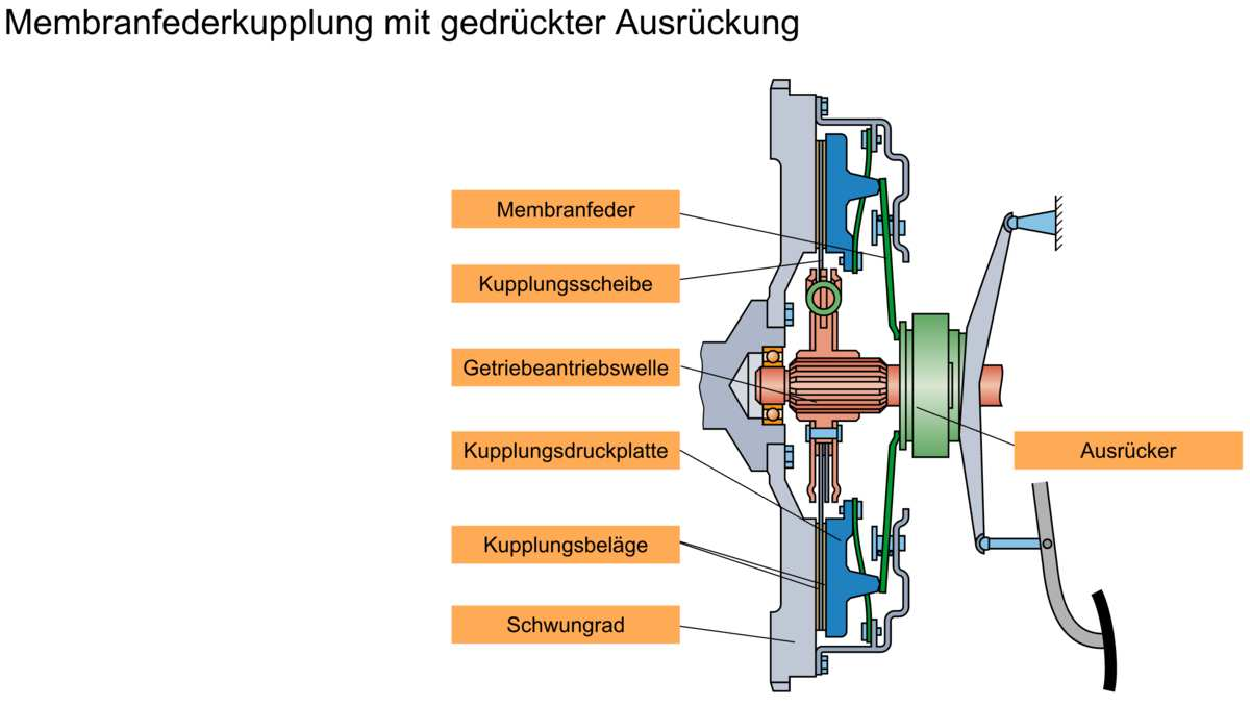
\includegraphics[width=0.7\textwidth]{images/Kupplung/Kupplung-8.pdf}
\caption{Kupplung, Quelle: Europa-Verlag}
%\label{fig:}%% anpassen
\end{figure}

Faktor 10, Ausrückhebel und Membranfederzungen 1 -- 3 mm, Leerweg am
Pedal 10 -- 30 mm

\textbf{manuellen Nachstellung}, das Seil wird mithilfe eines Gewindes
in eine neue Position gebracht. Am Pedal sollte ein Leerweg von etwa 10
bis 30 mm bleiben, um wärmebedingte Ausdehnungen zu kompensieren.

\textbf{Auswirkung von zu kleinem Kupplungsspiel}

\begin{enumerate}
\item
  Rutschen der Kupplung wegen geringer Anpresskraft der Membranfeder
\item
  Überhitzung der Kupplungsbeläge
\item
  Ausglühen der Membranfeder
\item
  Einlaufen der Membranfederspitzen
\item
  Punktuelle Überhitzung der Reibfläche am Schwungrad
\end{enumerate}

\textbf{Kraftfluss im eingekuppelten Zustand}

Kurbelwelle $\to$ Schwungrad $\to$ Druckplatte $\to$
Kupplungsscheibe $\to$ Getriebeantriebswelle

\textbf{Beschreibe den Vorgang des Auskuppelns}

\begin{enumerate}
\item
  Das Ausrücklager wird gegen den Innenrand der Membranfederzungen
  gedrückt.
\item
  Die Membranfeder wird in den Kippringen gekippt.
\item
  Die vorgespannten Tangentialplattfedern heben die Druckplatte ab.
\item
  Der Kraftfluss ist unterbrochen.
\end{enumerate}

\newpage

\section{Hydraulische
Kupplungsbetätigung}\label{hydraulische-kupplungsbetaetigung}

\begin{figure}[!ht]% hier: !ht
\centering
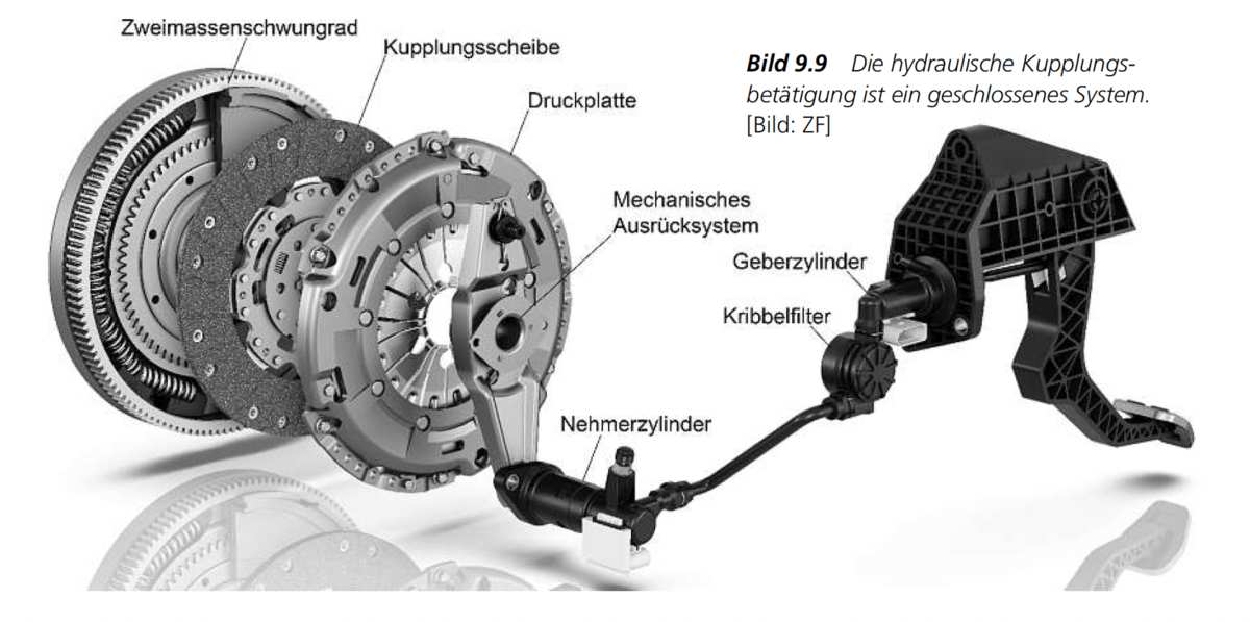
\includegraphics[width=0.7\textwidth]{images/Kupplung/Kupplung-1.pdf}
\caption{Hydraulische Kupplungsbetätigung, Quelle: Respondek}
%\label{fig:}%% anpassen
\end{figure}

\textbf{Vorteile}

\begin{enumerate}
\item
  Verstärkung durch hydraulische Übersetzung
\item
  Einfache Verlegung
\end{enumerate}

Der \textbf{Geberzylinder} erzeugt den Druck, der über den
\textbf{Nehmerzylinder} auf den Ausrückhebel, oder zentral geführt
direkt auf das Ausrücklager wirkt. In Ruhelage ist der Geberzylinder
über die Ausgleichsbohrung mit dem Ausgleichsbehälter, oftmals der von
der Bremse, verbunden. Somit kann die mit zunehmendem Belagverschleiß
überflüssige Bremsflüssigkeit dorthin entweichen und das System wird
selbstnachstellend. Bei einigen wenigen Fahrzeugen ist dennoch eine
Nachstellung des Endanschlags am Nehmerzylinder erforderlich.

Das System besitzt einen sog. Kribbelfilter (Schwingungsdämpfer), da der
Verbrennungsmotor die Kupplung durch seine Arbeitstakte zu Schwingungen
anregen kann, die sich durch das Ausrücksystem bis in das Pedal
fortsetzen. Diese Schwingungen würde der Fahrer als Kribbeln im Fuß
wahrnehmen.

\newpage

\section{Selbsteinstellende Kupplung (SAC -- Self Adjusting
Clutch)}\label{selbsteinstellende-kupplung-sac-self-adjusting-clutch}

\begin{figure}[!ht]% hier: !ht
\centering
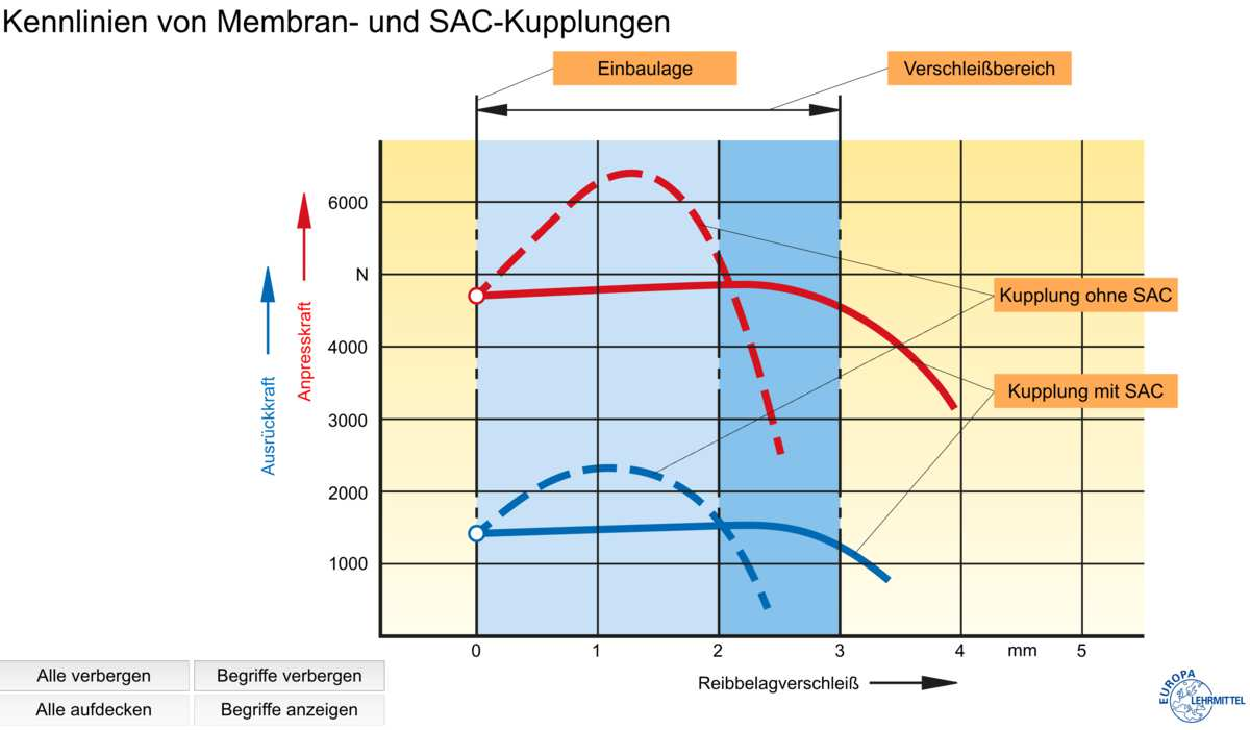
\includegraphics[width=0.7\textwidth]{images/Kupplung/Kupplung-6.pdf}
\caption{Kennlinien von Membran- und SAC-Kupplungen, Quelle:
Europa-Verlag}
%\label{fig:}%% anpassen
\end{figure}

\textbf{Vorteil}

\begin{itemize}
\item
  Schleifpunkt der Kupplung und die erforderliche Ausrückkraft, Pedal-
  und Anpresskräfte bleiben über den Belagverschleiß nahezu gleich.
  Größerer Belagverschleiß möglich.
\item
  die Kupplung stellt sich bei Belagverschleiß selbsttätig nach
\end{itemize}

\begin{figure}[!ht]% hier: !ht
\centering
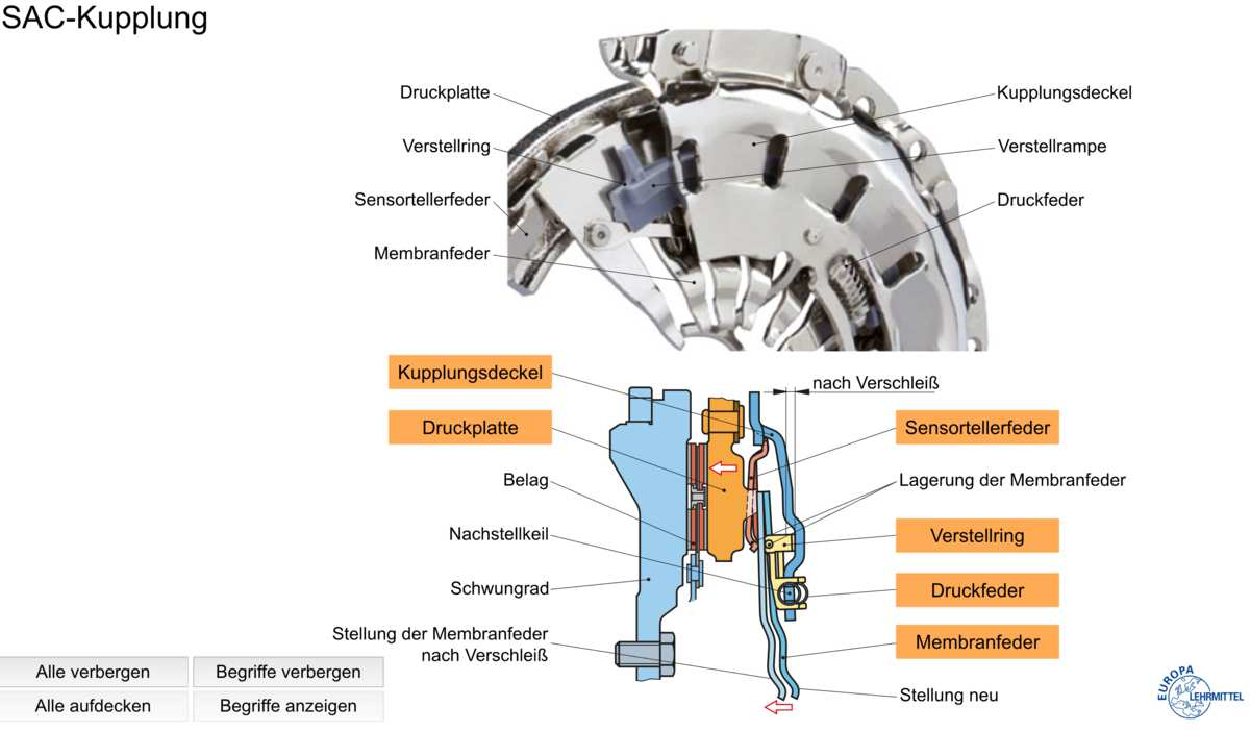
\includegraphics[width=0.7\textwidth]{images/Kupplung/Kupplung-7.pdf}
\caption{Selbsteinstellende Kupplung (SAC), Quelle: Europa-Verlag}
%\label{fig:}%% anpassen
\end{figure}

Durch eine Kombination der Membranfeder mit einer Sensor-Tellerfeder und
einem Verstellring.

\section{Kupplungsscheiben}\label{kupplungsscheiben}

\textbf{Nenne Aufgaben von Kupplungsscheiben}

\begin{enumerate}
\item
  Motordrehmomente übertragen vom Schwungrad auf die
  Getriebeeingangswelle
\item
  weiches und ruckfreies Anfahren ermöglichen
\item
  Drehschwingungen dämpfen
\end{enumerate}

\textbf{Welche Aufgabe haben die Belagfedern einer Kupplungsscheibe?}

\begin{itemize}
\item
  weiches und ruckfreies Anfahren ermöglichen
\item
  gleicht minimale Unebenheiten des Schwungrades und der Druckplatte
  aus, die ein Durchrutschen der Kupplung auslösen würde
\end{itemize}

\textbf{Welche Aufgabe haben die Torsionsfedern in einer
Kupplungsscheibe?}

\begin{itemize}
\item
  gleicht die Drehschwingungen des Motors aus
\item
  mindert Getriebegeräusche und Vibrationen
\end{itemize}

\newpage

\section{Störungssuche Kupplung}\label{stoerungssuche-kupplung}

\begin{figure}[!ht]% hier: !ht
\centering
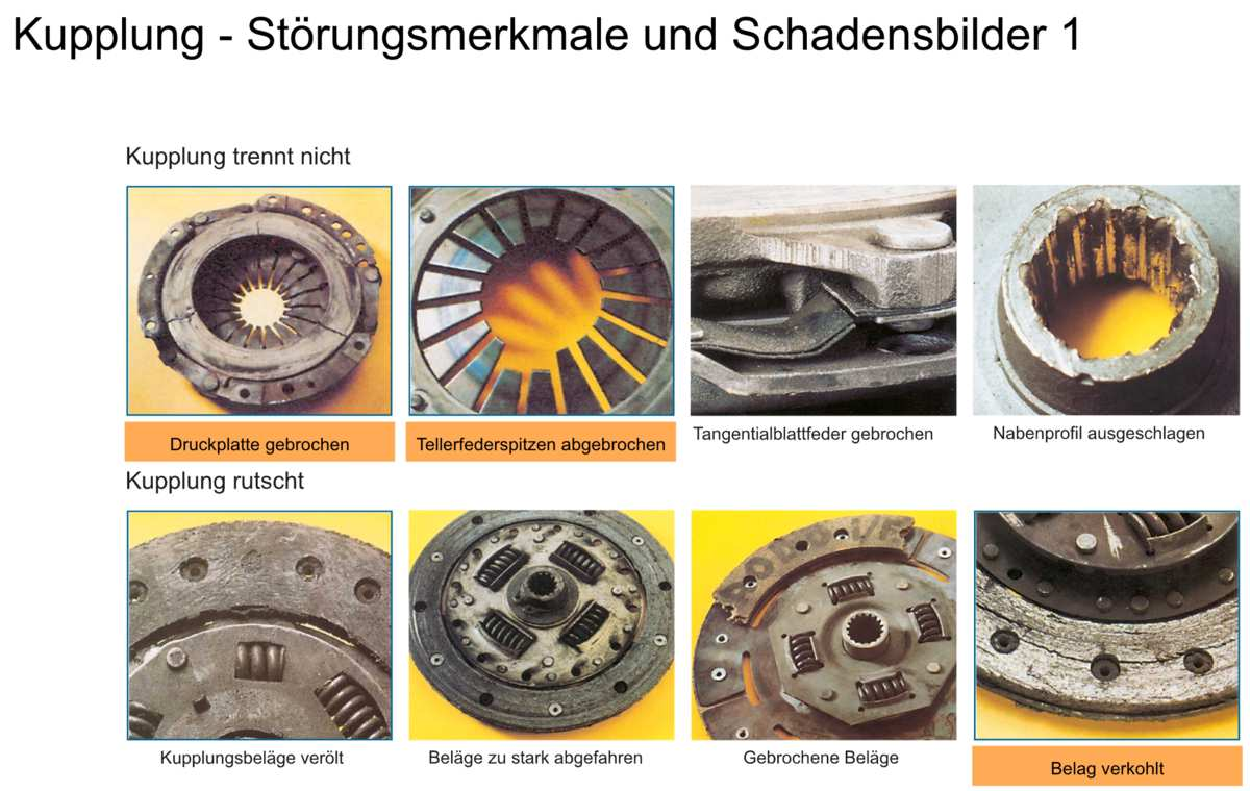
\includegraphics[width=0.7\textwidth]{images/Kupplung/Kupplung-5.pdf}
\caption{Kupplung rutscht oder trennt nicht, Quelle: Europa-Verlag}
%\label{fig:}%% anpassen
\end{figure}

\textbf{Kupplung rutscht}

\begin{enumerate}
\item
  Belag verschlissen
\item
  Belag verölt, verfettet
\item
  Belag überhitzt
\item
  Belag gebrochen
\item
  Schwungrad riefig/überhitzt
\item
  Druckplatte riefig/überhitzt
\item
  Kupplungsbetätigung schwergängig oder falsch eingestellt
\item
  Feder(n) gebrochen
\item
  SAC falsch eingebaut/eingestellt
\end{enumerate}

\textbf{Kupplung trennt nicht}

\begin{enumerate}
\item
  ZMS hat erhöhtes Axialspiel
\item
  Kupplungsbetätigung falsch eingestellt oder defekt
\item
  Nabe hängt auf der Getriebeeingangswelle (Schmutz/Rost/Beschädigung)
\item
  Seitenschlag der Kupplungsscheibe
\item
  Membranfeder/Ausrückhebel eingelaufen, verzogen oder gebrochen
\item
  Pilotlager schwergängig
\item
  Übermäßiges Axialspiel der Kurbelwelle
\item
  Kupplungsscheibe falsch eingebaut (Getriebe-/Motorseite)
\item
  Falsche Kupplungsscheibe eingebaut
\item
  SAC falsch eingebaut/eingestellt
\end{enumerate}

\textbf{Geräusche aus dem Kupplungsgehäuse}

\begin{figure}[!ht]% hier: !ht
\centering
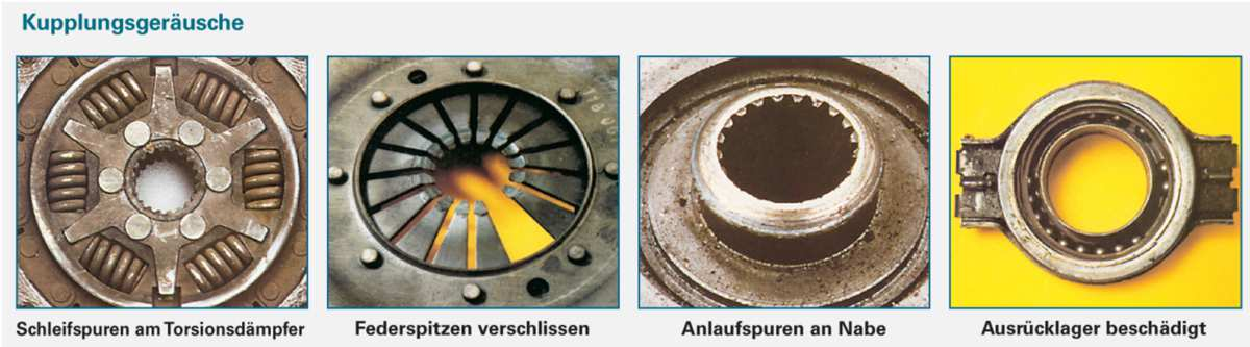
\includegraphics[width=0.7\textwidth]{images/Kupplung/Kupplung-3.pdf}
\caption{Kupplungsgeräusche, Quelle: Europa-Verlag}
%\label{fig:}%% anpassen
\end{figure}

\begin{enumerate}
\item
  ZMS defekt
\item
  Torsionsfeder/-dämpfereinrichtung der Kupplungsscheibe defekt
\item
  Ausrücklager defekt
\item
  Pilotlager defekt (Geräusche nur bei getrennter Kupplung)
\end{enumerate}

\textbf{Kupplung rupft}

\begin{figure}[!ht]% hier: !ht
\centering
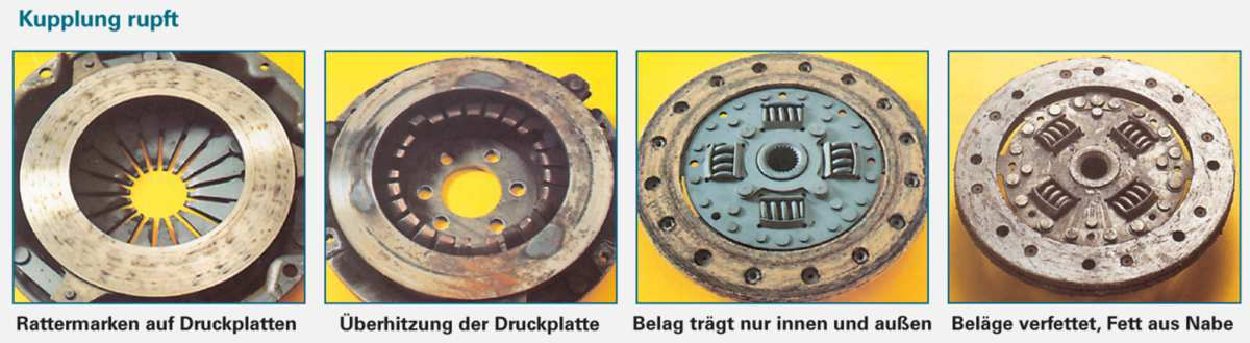
\includegraphics[width=0.7\textwidth]{images/Kupplung/Kupplung-2.pdf}
\caption{Kupplung rupft, Quelle: Europa-Verlag}
%\label{fig:}%% anpassen
\end{figure}

\begin{enumerate}
\item
  Beläge verölt/verfettet
\item
  Schwungrad riefig
\item
  Druckplatte riefig
\item
  Kupplungsgehäuse verzogen
\item
  Erhöhte Torsion im Antriebsstrang (Silentblöcke/Hardyscheibe)
\end{enumerate}

\section{Kupplung prüfen}\label{kupplung-pruefen}

\textbf{Auf Durchrutschen beim Anfahren}

\begin{enumerate}
\item
  Voraussetzung: Motor muss betriebswarm sein
\item
  Fahrzeug durch Feststellbremse sichern
\item
  Auskuppeln und höchsten Vorwärtsgang einlegen
\item
  Motordrehzahl bis zum Drehmomentmaximum erhöhen
\item
  Kupplung schnell einkuppeln und gleichzeitig Gas geben
\end{enumerate}

\textbf{Trennverhalten}

\begin{enumerate}
\item
  Voraussetzung: Motor, Getriebe, Kupplung sollte betriebswarm sein
\item
  Kupplungspedal durchtreten
\item
  3 -- 4 Sekunden warten
\item
  Rückwärtsgang einlegen und auf Geräusche achten
\end{enumerate}

\newpage

\section{Zweimassenschwungrad (ZMS)}\label{zweimassenschwungrad-zms}

\begin{figure}[!ht]% hier: !ht
\centering
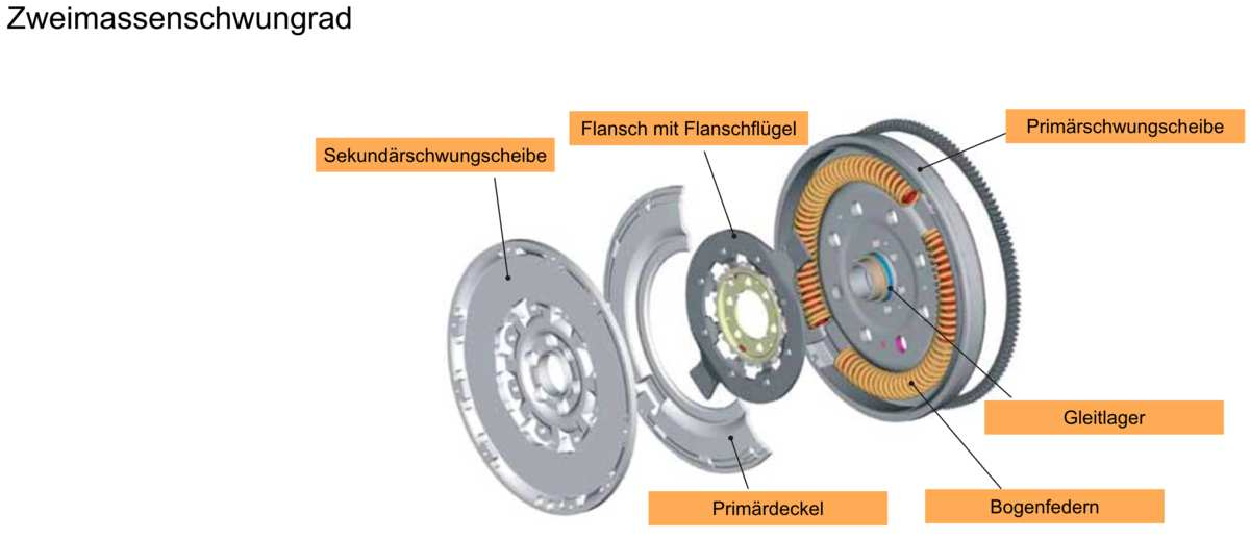
\includegraphics[width=0.7\textwidth]{images/Kupplung/Kupplung-9.pdf}
\caption{Zweimassenschwungrad, Quelle: Europa-Verlag}
%\label{fig:}%% anpassen
\end{figure}

\begin{figure}[!ht]% hier: !ht
\centering
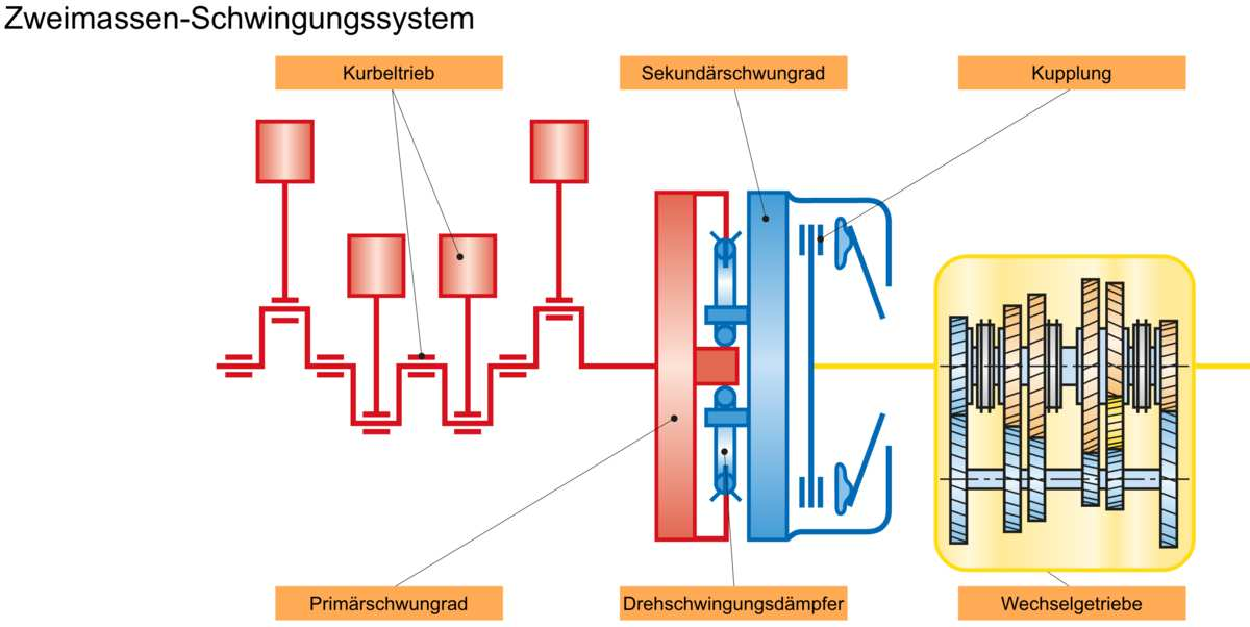
\includegraphics[width=0.7\textwidth]{images/Kupplung/Kupplung-10.pdf}
\caption{Zweimassenschwungrad, Quelle: Europa-Verlag}
%\label{fig:}%% anpassen
\end{figure}

\textbf{Wodurch erfolgt die Dämpfung der Drehschwingungen?}

Durch die Aufteilung der Schwungscheibe in einer Primär- und
Sekundärschwungmasse, die über Bogenfedern verbunden sind.

\chapter{13-Automatikgetriebe}
%%ju 26-Dez-22 13-Automatikgetriebe.tex
\section{Hauptsteuergrößen beim
Automatikgetriebe}\label{hauptsteuergroessen-beim-automatikgetriebe}

\begin{enumerate}
\item
  Fahrgeschwindigkeit
\item
  Fahrpedalstellung (Motorlast)
\item
  Wählhebelstellung
\item
  Motordrehzahl
\end{enumerate}

\textbf{Nebensteuergrößen}

\begin{enumerate}
\item
  Öltemperatur
\item
  Fahrertyp
\item
  Hängeretrieb oder Solo
\item
  Eingriff Fahrdynamikregelung
\end{enumerate}

\section{Arten von
Automatikgetriebe}\label{arten-von-automatikgetriebe}

\begin{enumerate}
\item
  Automatisierte Getriebe (ASG)

  \begin{itemize}
  \item
    Direktschaltgetriebe (DSG)
  \end{itemize}
\item
  gestufte Automatikgetriebe
\item
  stufenlose Automatikgetriebe (CVT)
\end{enumerate}

\begin{figure}[!ht]% hier: !ht
\centering
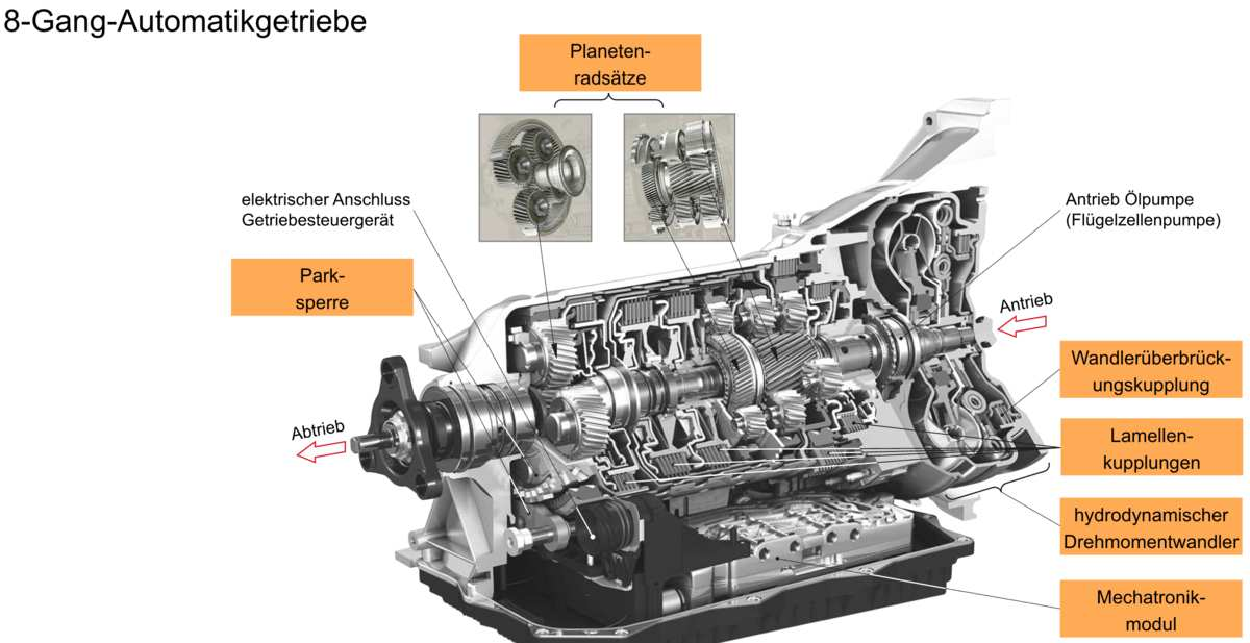
\includegraphics[width=0.7\textwidth]{images/Automatikgetriebe/Automatikgetriebe-1.pdf}
\caption{Automatikgetriebe, Quelle: Europa-Verlag}
%\label{fig:}%% anpassen
\end{figure}

\section{Fragen zum
Automatikgetriebe}\label{fragen-zum-automatikgetriebe}

\textbf{Aufgabe der Ölpumpe im Automatikgetriebe}

\begin{enumerate}
\item
  Wandler-Fülldruck
\item
  Schmierdruck für Planetengetriebe und Wandler
\item
  Arbeitsdruck zum Schalten der Lamellenkupplung
\end{enumerate}

\newpage

\textbf{Aufgabe eines hydrodynamischen Drehmomentwandlers}

\begin{enumerate}
\item
  Drehmoment wandeln und übertragen
\item
  Drehschwingungen vom Motor dämpfen
\item
  weiches und komfortables Anfahren ermöglichen
\end{enumerate}

\textbf{Überbrückungskupplung} Kraftfluss bei hohen Drehzahlen zwischen
Pumpenrad und Turbinenrad $\to$ Schlupf ausgleichen, Kraftstoff
sparen.

\textbf{Leitrad} bei unterer Drehzahl $\to$ Drehmomentverstärkung

\newpage

\textbf{Erklären Sie kurz gefasst die Wirkungsweise des hydrodynamischen
Drehmomentwandlers.}

\begin{figure}[!ht]% hier: !ht
\centering
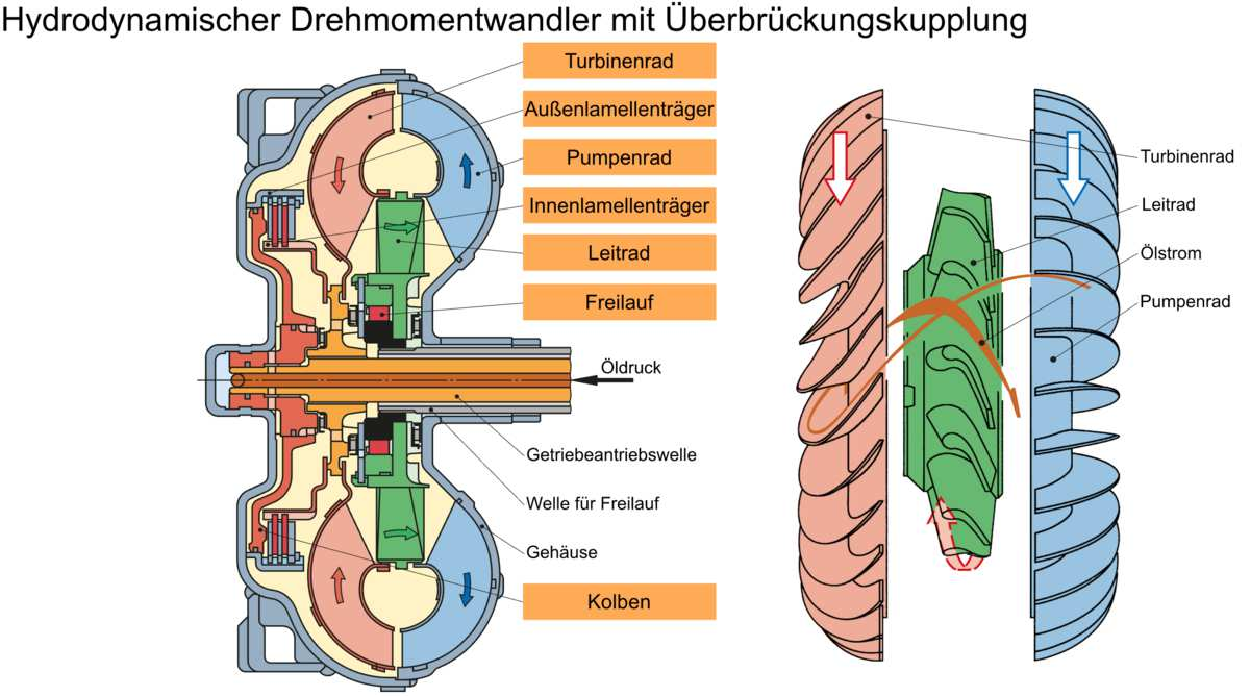
\includegraphics[width=0.7\textwidth]{images/Automatikgetriebe/Automatikgetriebe-2.pdf}
\caption{Hydrodynamischen Drehmomentwandler, Quelle: Europa-Verlag}
%\label{fig:}%% anpassen
\end{figure}

\begin{figure}[!ht]% hier: !ht
\centering
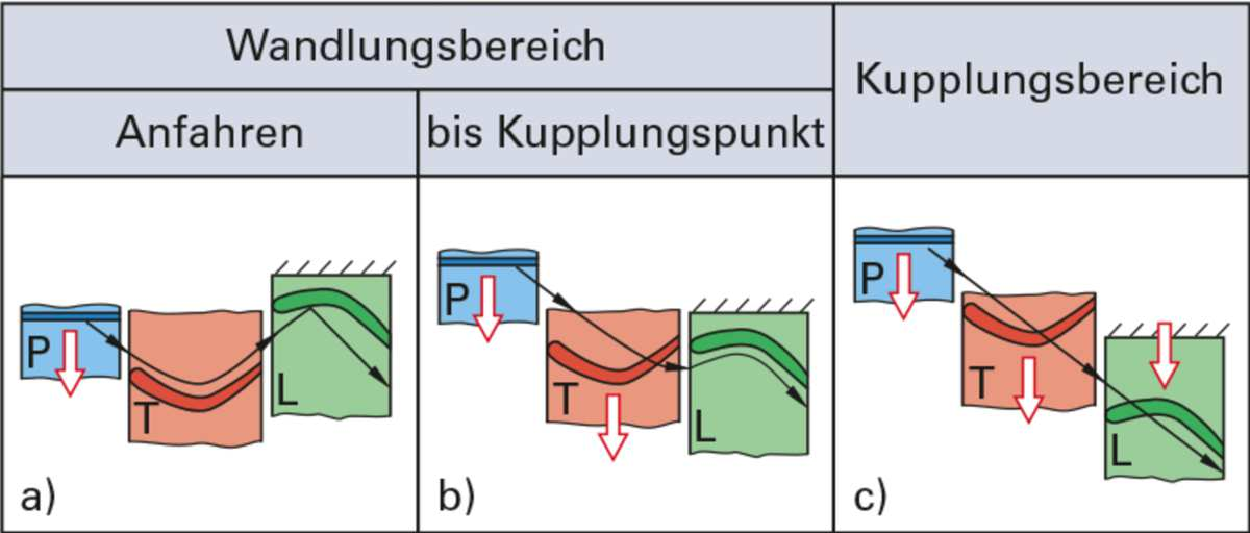
\includegraphics[width=0.4\textwidth]{images/Automatikgetriebe/Automatikgetriebe-3.pdf}
\caption{Drehmomentverstärkung, Quelle: Europa-Verlag}
%\label{fig:}%% anpassen
\end{figure}

\begin{table}[!ht]% hier: !ht 
\centering 
	\caption{}% \label{tab:}%% anpassen 
\begin{tabular}{@{}llll@{}}
\hline
\textbf{Wandlungsbereich} & \textbf{Anfahren} & \textbf{Kupplungspunkt}
& \textbf{Kupplungsbereich} \\
\hline
\textbf{Pumpenraddrehzahl} & Motordrehzahl & Motordrehzahl &
Motordrehzahl \\
\textbf{Turbinenraddrehzahl} & Null & Nimmt zu & > 85 \%
Pumpendrehzahl \\
\textbf{Leitraddrehzahl} & Null & Null & $\sim$ Turbinendrehzahl \\
\textbf{Ablenkwinkel des Ölstroms} & Groß & Klein & Keiner \\
\textbf{Drehmomenterhöhung} & Groß & Klein & Keine \\
\hline
\end{tabular} 
\end{table}

Je größer der Unterschied zwischen Pumpen- und Turbinenraddrehzahl,
desto größer ist die Drehmomenterhöhung.

\begin{figure}[!ht]% hier: !ht
\centering
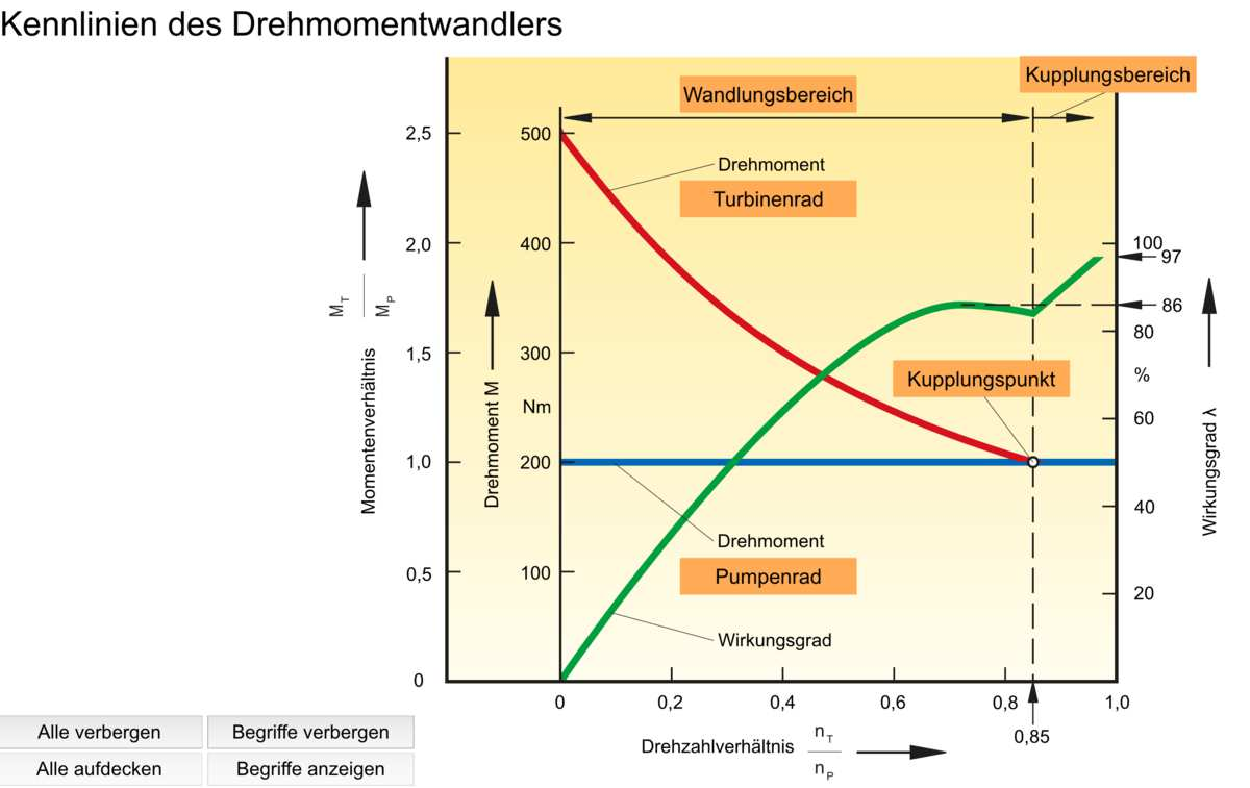
\includegraphics[width=0.7\textwidth]{images/Automatikgetriebe/Automatikgetriebe-4.pdf}
\caption{Kennlinien des Drehmomentwandlers, Quelle: Europa-Verlag}
%\label{fig:}%% anpassen
\end{figure}

Das Pumpenrad, mit der Motorkurbelwelle verbunden, versetzt das
Getriebeöl in strömende Bewegung. Das Turbinenrad, mit der
Getriebeeingangswelle verbunden, wird durch das strömende Getriebeöl
mitgenommen. Das Leitrad stützt sich über einen Freilauf entgegen der
Motordrehrichtung ab und lenkt den Ölstrom strömungsgünstig auf das
Pumpenrad zurück. Hierdurch kommt es zu einer Unterstützung des
Pumpenrades und damit zu einer Drehmomentverstärkung um bis zu 150 \%.
Die Drehmomentverstärkung ist proportional zur Drehzahldifferenz
zwischen Pumpen- und Turbinenrad. Beträgt die Drehzahl des Turbinenrades
etwa 85 \% der Drehzahl des Pumpenrades, ist der Kupplungspunkt
erreicht. Bei weiterem Drehzahlanstieg arbeitet der Wandler nur noch als
hydrodynamische Kupplung, weil sich das Leitrad durch den Freilauf
gelöst hat und frei mit dreht. Die Drehmomentverstärkung entfällt.

\textbf{Was versteht man unter der Festbremsdrehzahl bei einem
Automatikfahrzeug?}

\begin{itemize}
\item
  Es ist, die vom Hersteller angegebene Drehzahl, die ein Motor unter
  Volllaststellung am Fahrpedal bei eingelegter Fahrstufe und betätigter
  Betriebs- und Feststellbremse erreichen muss, ohne sie zu
  überschreiten. Die Prüfzeit darf max. 5 s betragen.
\item
  Mögliche Ursachen bei zu geringer Drehzahl:

  \begin{itemize}
  \item
    Wandlerfreilauf rutscht durch
  \item
    Störung im Motor (Keine Leistung)
  \end{itemize}
\item
  Mögliche Ursachen bei zu hoher Drehzahl:

  \begin{itemize}
  \item
    Wandler stellt keinen vollständigen Kraftschluss her (Ölstand?)
  \item
    Getriebe rutscht durch (Drehzahl Getriebeeingang prüfen)
  \end{itemize}
\end{itemize}

\newpage

\textbf{Wie werden Automatikgetriebe grundsätzlich geschaltet?}

\begin{itemize}
\item
  Automatikgetriebe werden grundsätzlich hydraulisch geschaltet. Das
  Schalten erfolgt durch das Schließen und Öffnen von Lamellenkupplungen
  und --bremsen, sowie, bei älteren Getriebevarianten, Bremsbändern.
\item
  Während ältere Getriebe oftmals hydropneumatisch in Abhängigkeit von
  Motordrehzahl (\textbf{Arbeitsdruck}), Last (\textbf{Modulierdruck})
  und Fahrgeschwindigkeit (\textbf{Reglerdruck}) gesteuert wurden,
  erfolgt die Steuerung heutzutage meistens elektronisch über die
  elektrohydraulische Steuereinheit. Hierbei werden bei der Definition
  der Schaltpunkte nicht nur die Hauptsteuergrößen Motordrehzahl, Last
  und Fahrgeschwindigkeit, sondern auch Nebensteuergrößen, wie z.B.
  Öltemperatur, Fahrertyp (sportlich, defensiv~\ldots),
  Betriebsbedingungen (Solo, Hängerbetrieb~\ldots), Eingriff
  Fahrdynamikregelung usw. berücksichtigt.
\end{itemize}

\newpage

\textbf{Aus welchen Teilen besteht der Planetenradsatz eines
Planetengetriebes und wie sind diese Teile angeordnet?}

\begin{figure}[!ht]% hier: !ht
\centering
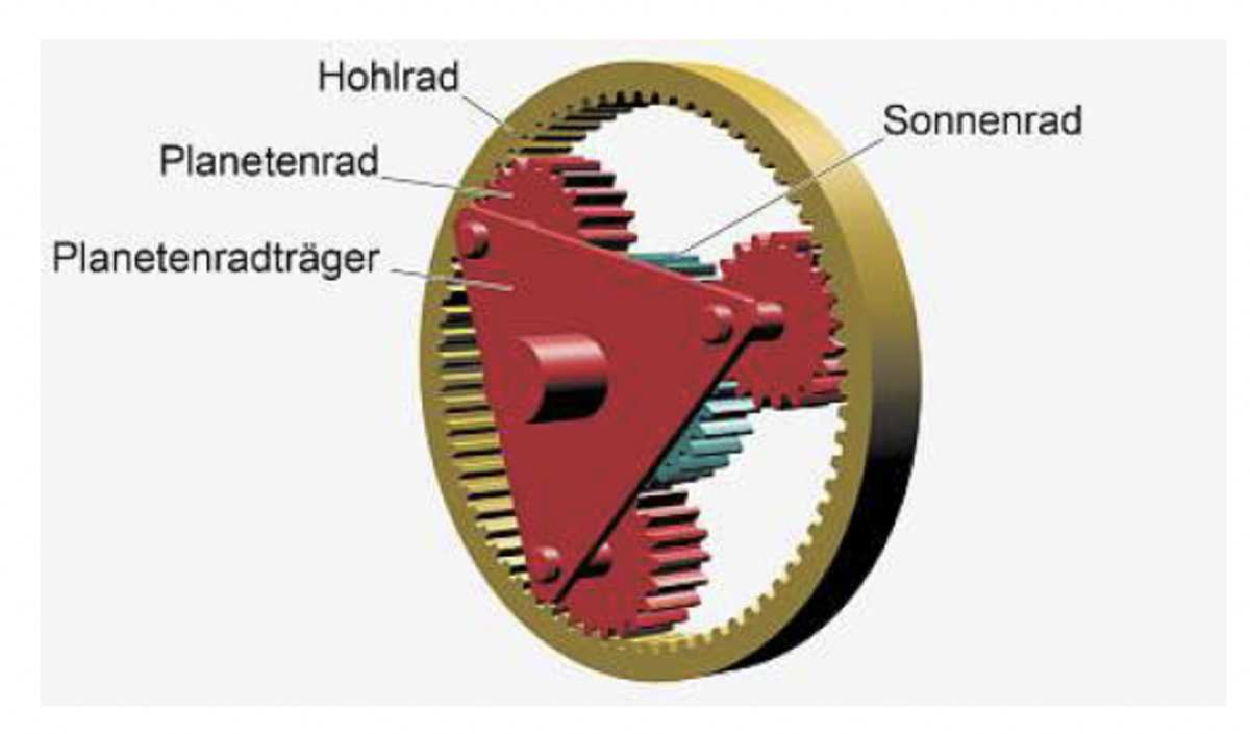
\includegraphics[width=0.3\textwidth]{images/Automatikgetriebe/Automatikgetriebe-6.pdf}
\caption{Planetenradsatz, Quelle: Europa-Verlag}
%\label{fig:}%% anpassen
\end{figure}

Zentrales Bauelement des einfachen Planetenradsatzes ist das Sonnenrad.
Auf diesem laufen Planetenräder, die ihrerseits durch den
Planetenradträger untereinander verbunden sind. Die Planetenräder werden
vom Hohlrad umschlossen, in welchem sie ebenfalls ablaufen können.

\textbf{Welchen Vorteil hat ein Planetengetriebe gegenüber einem
Schaltgetriebe?}

Es lässt sich unter Last schalten, d.h. zum Schalten ist keine
Trennkupplung zwischen Motor und Getriebe erforderlich.

\textbf{Was ist die Voraussetzung für die Kraftübertragung?}

\begin{enumerate}
\item
  Möglichkeit: 1x Antrieb (Antriebskupplungen), 1x fest gebremst
  (Bremskupplungen), 1x Abtrieb
\item
  Möglichkeit: 2x angetrieben, 1x Abtrieb
\end{enumerate}

\begin{figure}[!ht]% hier: !ht
\centering
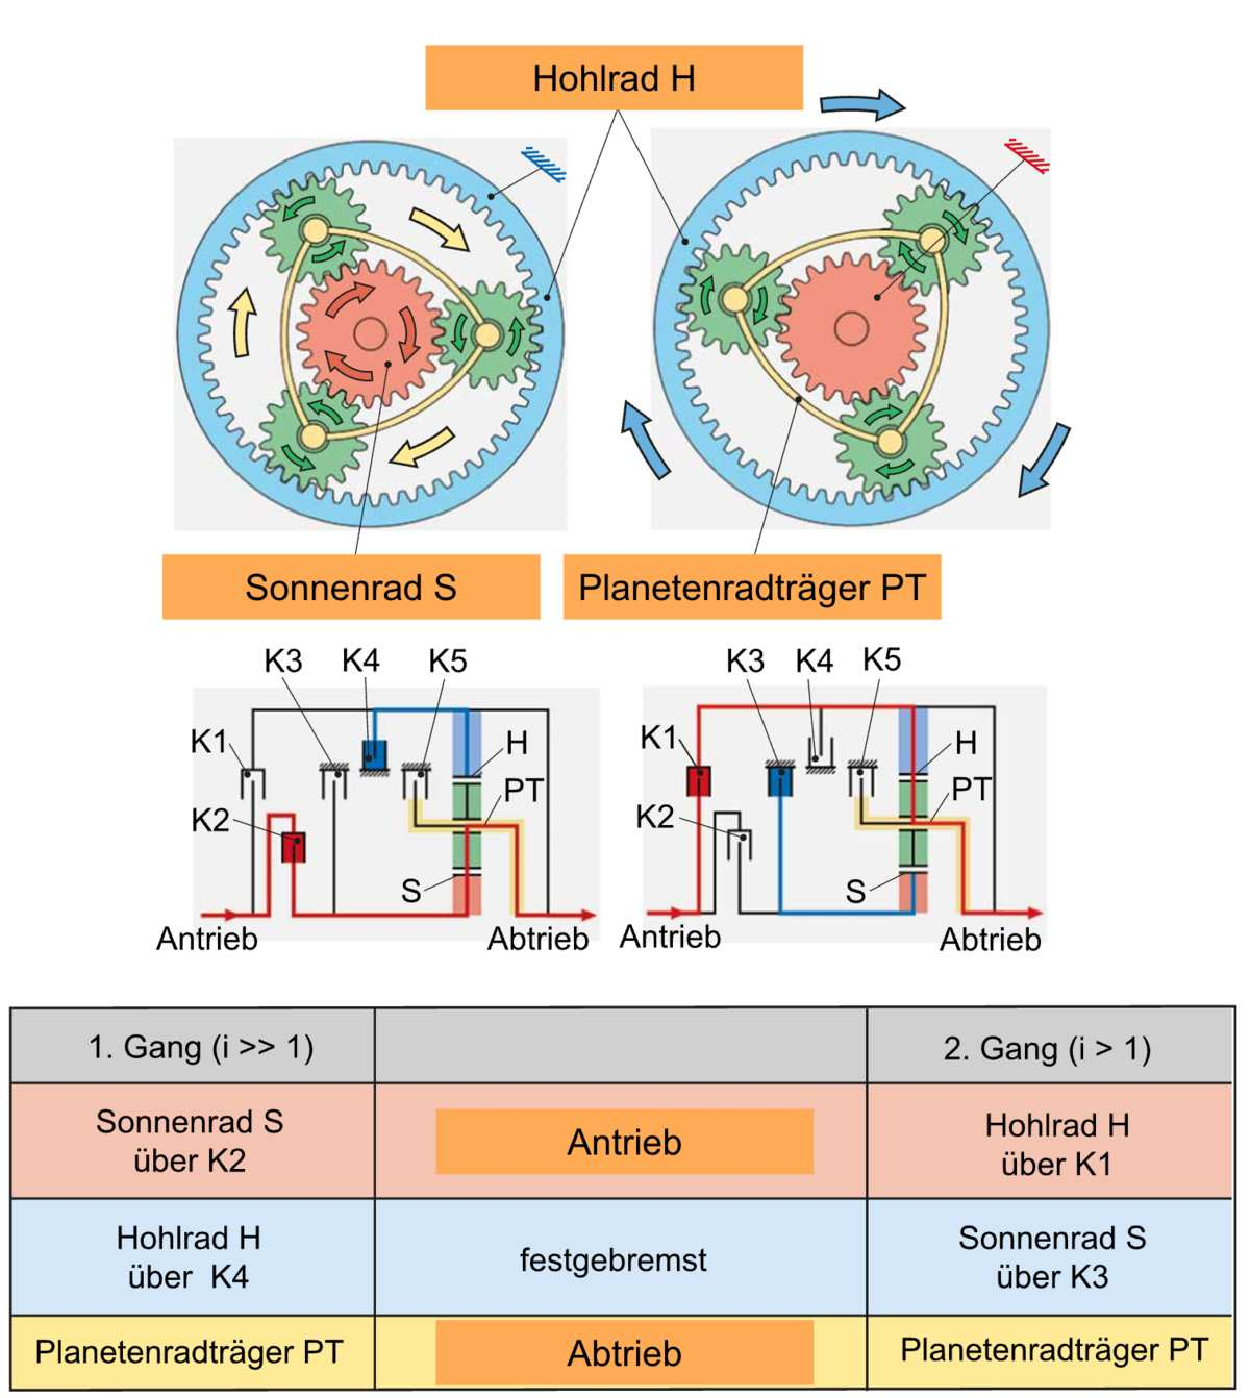
\includegraphics[width=0.4\textwidth]{images/Automatikgetriebe/Automatikgetriebe-5.pdf}
\caption{Kraftübertragung, Quelle: Europa-Verlag}
%\label{fig:}%% anpassen
\end{figure}

\newpage

\textbf{Worin unterscheiden sich die Planetengetriebe Simpson und
Ravigneaux?}

\begin{figure}[!ht]% hier: !ht
\centering
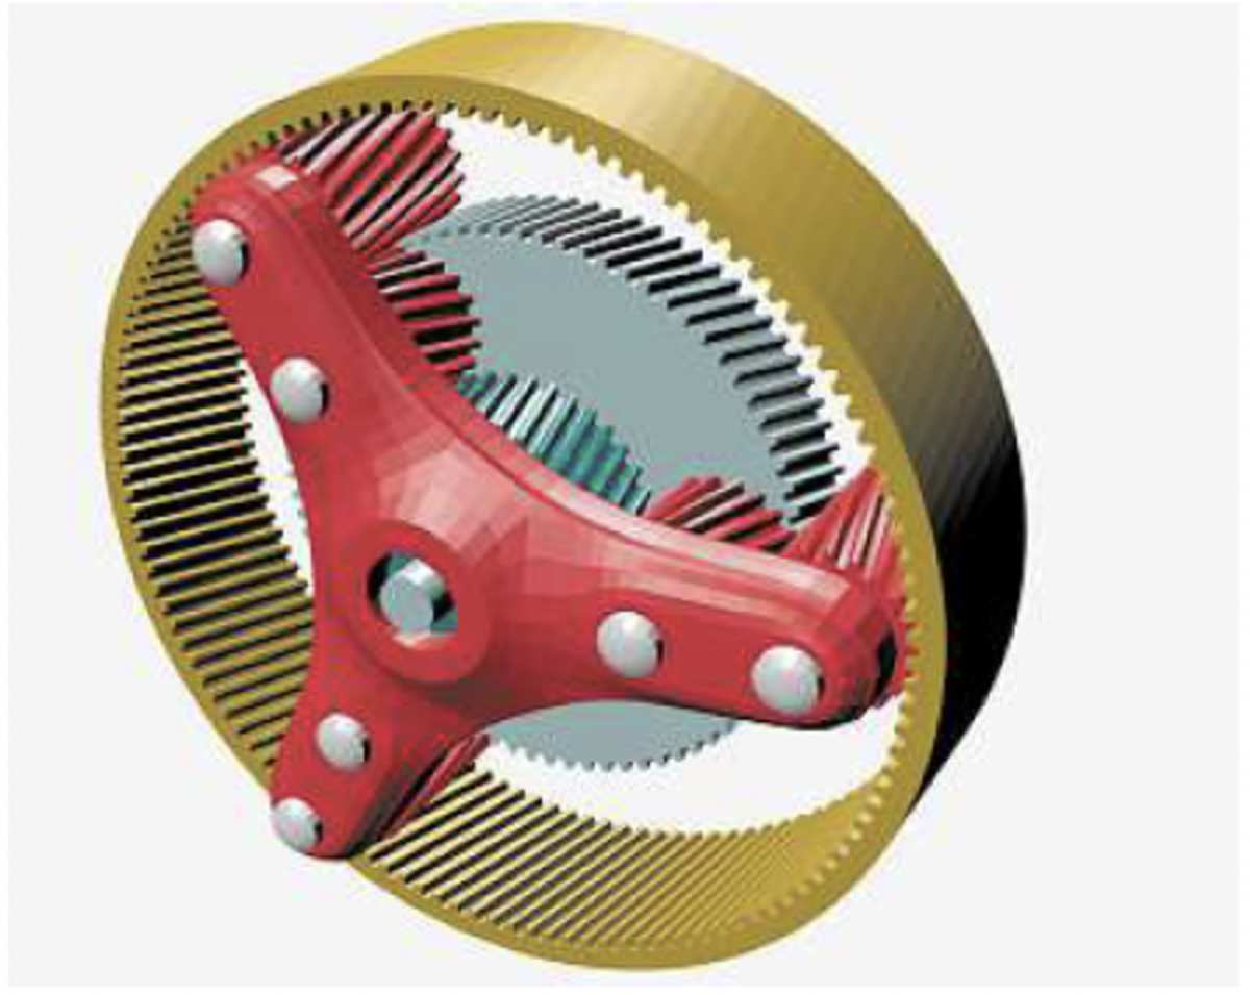
\includegraphics[width=0.3\textwidth]{images/Automatikgetriebe/Automatikgetriebe-7.pdf}
\caption{Ravigneaux-Planetengetriebe, Quelle: Europa-Verlag}
%\label{fig:}%% anpassen
\end{figure}

\begin{figure}[!ht]% hier: !ht
\centering
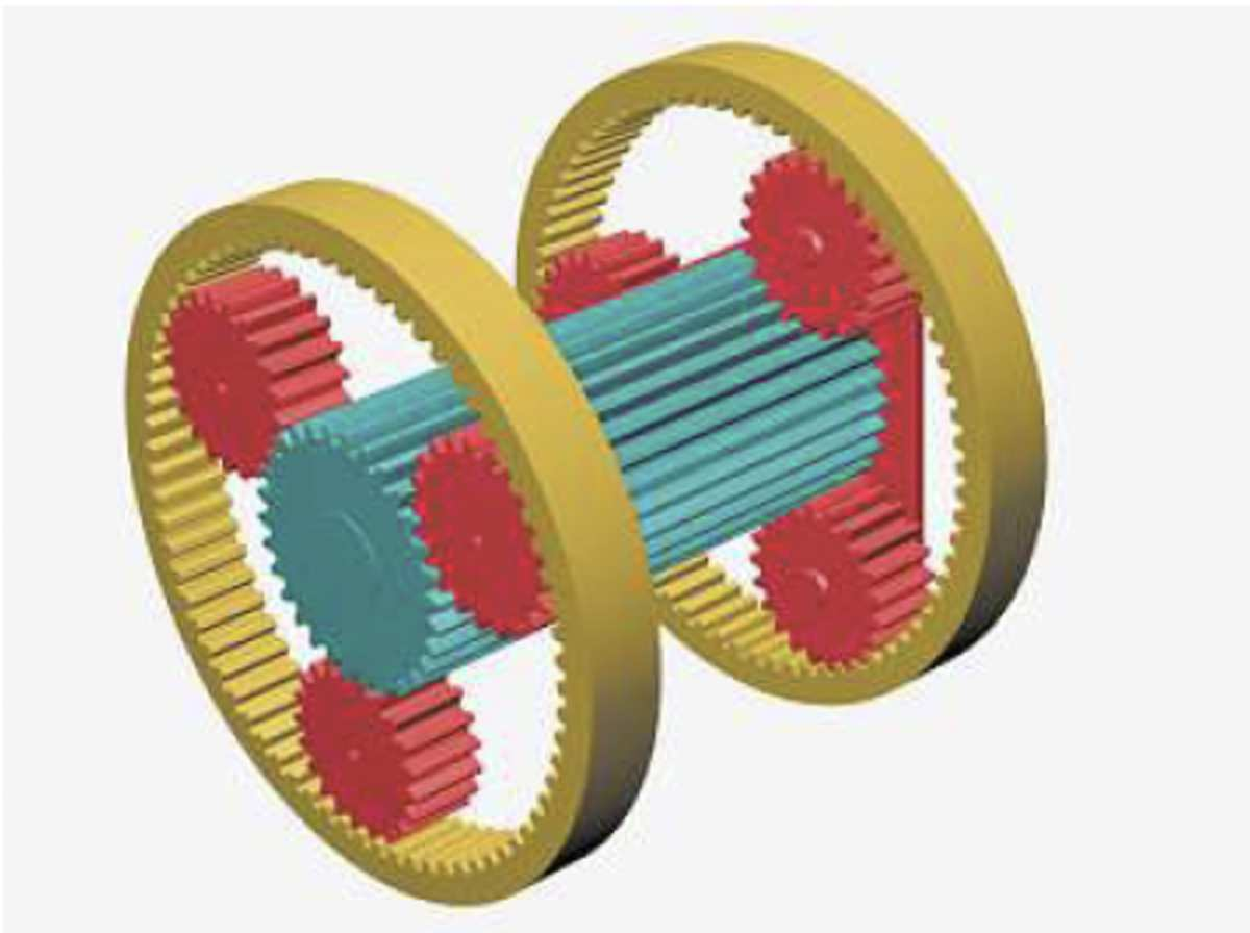
\includegraphics[width=0.3\textwidth]{images/Automatikgetriebe/Automatikgetriebe-8.pdf}
\caption{Simpson-Planetengetriebe, Quelle: Europa-Verlag}
%\label{fig:}%% anpassen
\end{figure}

\begin{itemize}
\item
  Das Simpson-Planetengetriebe besteht aus zwei Planetenradsätzen, die
  sich ein Sonnenrad teilen.
\item
  Beim Ravigneaux-Planetengetriebe teilen sich zwei Planetenradsätze ein
  gemeinsames Hohlrad.
\end{itemize}

\newpage

\textbf{Beschreiben Sie die Wirkungsweise einer Lamellenkupplung in
einem Automatikgetriebe.}

\begin{figure}[!ht]% hier: !ht
\centering
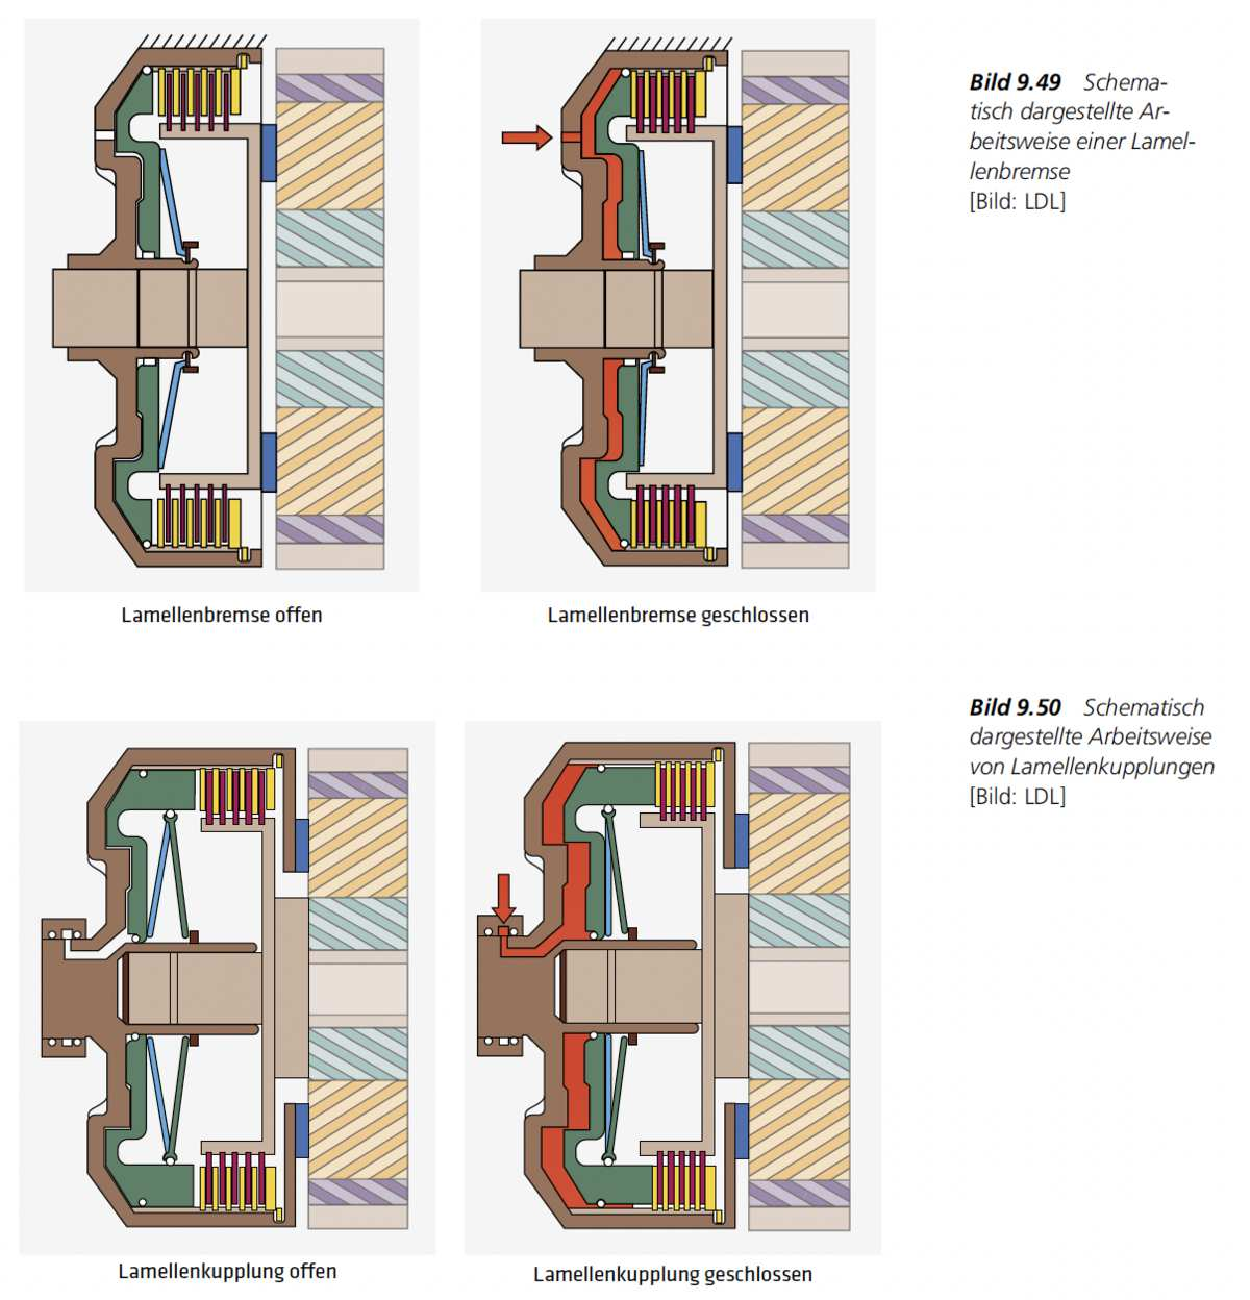
\includegraphics[width=0.7\textwidth]{images/Automatikgetriebe/Automatikgetriebe-12.pdf}
\caption{Lamellenkupplung, Quelle: Europa-Verlag}
%\label{fig:}%% anpassen
\end{figure}

Über eine beidseitig abgedichtete Wellenbohrung gelangt das Getriebeöl
unter Druck hinter den Kolben der Lamellenkupplung. Dieser fährt aus und
presst das Lamellenpaket, welches aus formschlüssig mit dem
Außenlamellenträger verbundenen Außenlamellen und formschlüssig mit dem
Innenlamellenträger verbundenen Innenlamellen besteht zusammen. Beide
Bauteile werden nun kraftschlüssig und drehen sich gleichmäßig oder mit
definiertem Schlupf. Zum Lösen der Kupplung wird der Druck abgebaut,
wodurch der Kolben mithilfe einer Tellerfeder in die Ausgangslage
gedrückt wird. Um zu verhindern, dass es durch das, der Fliehkraft
ausgesetzte Öl im Kolbenraum zu einer Betätigung der Kupplung kommt,
gibt es vor dem Kolben eine Kolbenabdeckung, die als Gegenkolben wirkt
und die Ruhelage des Kolbens sicherstellt.

\newpage

\textbf{Wozu dienen die 1. und falls vorhanden, die 2. Ölpumpe im
Automatikgetriebe?}

\begin{enumerate}
\item
  Aufgaben der 1. Ölpumpe

  \begin{itemize}
  \item
    Befüllung des Wandlers oder der Kupplung mit Getriebeflüssigkeit
  \item
    Schmierölversorgung der Planetengetriebe
  \item
    Belieferung der Steuereinheit mit, unter Druck stehendem Getriebeöl
  \item
    Betätigung der Lamellenkupplungen und -bremsen
  \end{itemize}
\item
  Aufgabe der 2. Ölpumpe

  \begin{itemize}
  \item
    Schmierölversorgung beim Abschleppen
  \end{itemize}
\item
  Aufgabe der elektrischen Ölpumpe

  \begin{itemize}
  \item
    Druckerhalt im Getriebe im Start-Stopp-Betrieb
  \end{itemize}
\end{enumerate}

\textbf{Wie ist die Wirkungsweise einer Parksperre?}

\begin{figure}[!ht]% hier: !ht
\centering
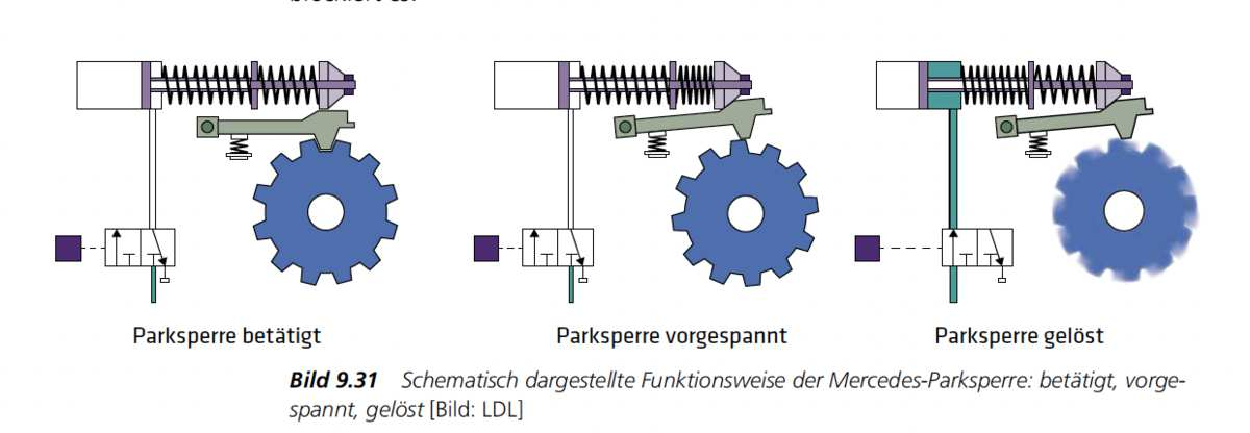
\includegraphics[width=0.7\textwidth]{images/Automatikgetriebe/Automatikgetriebe-9.pdf}
\caption{Parksperre, Quelle: Europa-Verlag}
%\label{fig:}%% anpassen
\end{figure}

Bei Betätigung des Wählhebels in Stellung >>P<<, wird über ein Gestänge,
einen Bowdenzug oder einen Stellmotor, eine mechanische Sperrklinke
freigegeben, die sich in das, mit der Getriebeabtriebswelle verbundene
Parksperrenrad einhakt und so die Getriebeabtriebswelle blockiert.

\textbf{Was versteht man unter einer adaptiven elektrohydraulischen
Getriebesteuerung?}

Darunter versteht man die Anpassung der elektrohydraulischen
Getriebesteuerung an die Einsatzbedingungen des Fahrzeugs, den Fahrstil
des Fahrers und den Verschleiß im Getriebe. Das Steuergerät ist
selbstlernend und passt die Schaltzeitpunkte und die Drücke im Getriebe
so an, dass eine konstant hohe Schaltqualität gewährleistet werden kann.

\textbf{Lassen sich Fahrzeuge mit einem vollautomatischen Getriebe
anschleppen?}

Das Anschleppen ist im Normalfall nicht möglich, da zum Schalten der
Gänge hydraulischer Druck erforderlich ist. Da der Motor nicht läuft,
fördert auch die 1. Ölpumpe nicht. Die Ausnahme besteht bei
Automatikgetrieben mit 2. Ölpumpe, die von der Getriebeabtriebswelle
angetrieben wird.

\chapter{14-Antrieb}
%%ju 31-Dez-22 14-Antrieb.tex
\textbf{Wie ist eine Viscokupplung aufgebaut?}

\begin{itemize}
\item
  Ein zylindrisches, mit dem Antrieb verbundenes Gehäuse
\item
  Gelochte Außenlamellen, drehfest mit dem Gehäuse verbunden
\item
  Innenlamellen, drehfest mit der Abtriebswelle verbunden
\item
  Füllung mit hochviskoser Silikonflüssigkeit.
\end{itemize}

\textbf{Warum sind bei einer Gelenkwelle 2 Kreuzgelenke erforderlich?}

Kreuzgelenke sind nicht homokinetisch. Nach dem ersten gebeugten
Kreuzgelenk ist aus der ursprünglich gleichförmigen Bewegung der Welle
eine ungleichförmige Bewegung geworden.

Um diesen Effekt wieder auszugleichen benötigt man ein zweites
Kreuzgelenk, dessen Gelenkgabel in derselben Ebene, wie die des ersten
liegen muss.

\textbf{Was sind homokinetische Gelenke? Nennen Sie mindestens 3
homokinetische Gelenke mit Ihren spezifischen Eigenschaften.}

Homokinetische Gelenke sind Gleichlaufgelenke. Durch ihren Einsatz kommt
es zu keinerlei Veränderungen in der radialen Bewegung der Welle.

\begin{enumerate}
\item
  \textbf{Kugelgelenk} Beugewinkel bis zu 38° (47°), keine axiale
  Verschiebung möglich
\item
  \textbf{Topfgelenk} Beugewinkel bis zu 22°, axiale Verschiebung um
  max. 45 mm
\item
  \textbf{Tripodegelenk} Beugewinkel bis zu 26°, axiale Verschiebung um
  max. 55 mm
\item
  \textbf{Doppelgelenk} Beugewinkel bis zu 50°, keine axiale
  Verschiebung möglich
\item
  \textbf{Gewebescheibengelenk} (Hardyscheibe) Beugewinkel bis zu 5°,
  axiale Verschiebung um max. 1,5 mm
\end{enumerate}

\textbf{Welcher Unterschied besteht zwischen}

\textbf{a) dem normalen Kegelradantrieb?} \textbf{b) dem Hypoidantrieb?}

\begin{enumerate}
\item
  Beim normalen Kegelradantrieb liegen die Achsen von Teller und
  Kegelrad in einer Ebene.
\item
  Beim Hypoidantrieb ist die Mittellinie des Kegelrades gegenüber der
  Mittellinie des Tellerrades nach unten versetzt.

  \begin{itemize}
  \item
    größere Kraftübertragung, da mehr Zähne im Eingriff
  \item
    Gelenkwelle kann nach unten versetzt werden

    \begin{itemize}
    \item
      $\to$ niedrigerer Schwerpunkt des Fahrzeugs
    \item
      $\to$ flacherer Gelenkwellentunnel
    \end{itemize}
  \end{itemize}
\end{enumerate}

\textbf{Aus welchem Grund ist beim Kraftfahrzeug ein Ausgleichsgetriebe
erforderlich?}

Das Ausgleichsgetriebe ist notwendig, um die Wegunterschiede
auszugleichen, die bei Kurvenfahrt zwischen dem kurveninneren Rad
(kleiner Radius und damit Umfang) und dem kurvenäußeren Rad (großer
Radius und damit Umfang) liegen.

Würde dies nicht geschehen,

\begin{itemize}
\item
  würde das Fahrzeug stark untersteuern
\item
  würden die Räder Schlupf aufweisen und entsprechende Geräusche
  entstehen
\item
  würden Bauteile durch die starken Torsionskräfte zerstört
\end{itemize}

\textbf{Wie ist die Wirkungsweise des Ausgleichsgetriebes bei
Geradeausfahrt?}

Das Tellerrad mit angeflanschtem Ausgleichsgehäuse wird vom Kegelrad
angetrieben. Vom drehenden Ausgleichsgehäuse werden der fest angeordnete
Differentialbolzen bzw. das Differentialkreuz und die, auf ihm
gelagerten Ausgleichskegelräder mitgenommen. Die Ausgleichskegelräder,
die mit den Achswellenkegelrädern im Eingriff sind, treiben diese an,
ohne sich um ihre eigene Achse zu drehen.

\textbf{Wie verhält sich das Ausgleichsgetriebe beim Anfahren mit
Schlupf?}

Das übertragene Antriebsmoment ist an beiden Rädern grundsätzlich gleich
groß. Hat also eines der Räder Schlupf, verringert sich das, an dem
anderen Rad übertragene Antriebsmoment. Liegt der Schlupf bei 100 \%,
das Rad dreht also durch, fällt der Vortrieb des Fahrzeuges weg, da das
andere Rad stehen bleibt.

\textbf{Wie ist die Wirkungsweise eines Selbstsperrdifferentials?}

Das Ausgleichsgehäuse besteht in diesem Differential aus zwei Teilen,
zwischen denen das Differentialkreuz gelagert ist. Kommt es im
Ausgleichsgetriebe zu Drehzahldifferenzen, so drücken die, durch das
Drehen der Ausgleichskegelräder entstehenden Spreizkräfte das
Ausgleichsgehäuse auseinander und pressen damit eine, zwischen den
Gehäusehälften und dem umfassenden Käfig gelagerte Lamellenkupplung
zusammen, die die Antriebswellen mit dem Gehäuse verbindet. Die Sperrung
des Differential ist proportional zur Drehzahldifferenz, wodurch der
maximale Sperrwert bei etwa 70 \% liegt.

\chapter{15-CVT-Automatikgetriebe}
%%ju 26-Dez-22 15-CVT-Automatikgetriebe.tex
\textbf{Worin unterscheidet sich das stufenlose Automatikgetriebe CVT
von den herkömmlichen Automatikgetrieben?}

\begin{itemize}
\item
  Das CVT-Automatikgetriebe (Continuously Variable Transmission) hat
  keine Fahrstufen, sondern über den gesamten Fahrbereich eine
  stufenlose Übersetzung.
\end{itemize}

\textbf{Wie ist die Wirkungsweise des CVT-Automatikgetriebes?}

\begin{itemize}
\item
  Das Drehmoment wird über die Antriebswelle und den Planetenradsatz auf
  die Primärkegelscheibe und von dort über ein Schubgliederband oder
  eine Laschenkette auf die Sekundärkegelscheibe und die Abtriebswelle
  übertragen. Durch das wechselseitige Verändern der wirksamen Radien an
  Primärund Sekundärkegelscheibe wird das Übersetzungsverhältnis
  stufenlos angepasst.
\end{itemize}

\textbf{Wie wird das Übersetzungsverhältnis beim CVT-Automatikgetriebe
verändert?}

\begin{itemize}
\item
  Das Übersetzungsverhältnis lässt sich durch das gegenläufige Verändern
  der Durchmesser von Primär- und Sekundärkegelscheibe stufenlos
  bestimmen. Jeweils eine Scheibenhälfte der Primär- sowie der
  Sekundärkegelscheibe lässt sich durch hydraulischen Druck axial
  verschieben. Wird z.B. eine Primärkegelscheibenhälfte hydraulisch
  beaufschlagt und axial verschoben, so vergrößert sich dadurch der
  wirksame Radius für die Schubgliederlaufbahn. Gleichzeitig wird an der
  Sekundärkegelscheibenhälfte der hydraulische Druck verringert und der
  wirksame Radius verkleinert.
\end{itemize}

\textbf{Wann ist bei einem CVT-Automatikgetriebe das
Übersetzungsverhältnis am größten?}

\begin{itemize}
\item
  Das Übersetzungsverhältnis ist am größten, wenn an der
  Primärkegelscheibe der kleinste und an der Sekundärkegelscheibe der
  größte Durchmesser eingestellt ist.
\end{itemize}

\textbf{Worin unterscheidet sich die stufenlose Multitronic (Audi) von
der herkömmlichen stufenlosen CVT-Automatik?}

\begin{itemize}
\item
  Statt des Schubgliederbandes wird eine Laschenkette verwendet

  \begin{itemize}
  \item
    Größere übertragbare Zugkräfte (bis zu 1,7 t)
  \item
    Durch flachere Bauweise größerer Verstellbereich an den
    Kegelscheiben
  \item
    Größerer Übersetzungsfaktor zwischen der größten und der kleinsten
    Übersetzung (6,05)
  \end{itemize}
\item
  Nach dem Tiptronic -- Muster können 6 feste Gangstufen simuliert
  werden.
\item
  Das dynamische Regelprogramm der Steuerelektronik ist selbstlernend,
  es passt sich dem Fahrstil zwischen >>sportlich<< und
  >>wirtschaftlich<< an.
\end{itemize}

\chapter{16-Direktschaltgetriebe}
%%ju 31-Dez-22 16-Direktschaltgetriebe.tex
\textbf{Woraus besteht das Direktschaltgetriebe?}

\begin{itemize}
\item
  Es besteht im Prinzip aus 2 Teilgetrieben. Jedes Teilgetriebe ist in
  seiner Wirkung wie ein Handschaltgetriebe aufgebaut. Jedem
  Teilgetriebe ist eine Kupplung zugeordnet. Die beiden Eingangswellen
  sind als hohle Außen- und volle Innenwelle ausgeführt. Alle
  Übersetzungsstufen sind, wie bei normalen Schaltgetrieben, als
  Zahnradpaare auf Eingangs- und Nebenwellen untergebracht.
\end{itemize}

\textbf{Wie sind die 6 Gänge im Direktschaltgetriebe angeordnet?}

\begin{itemize}
\item
  Auf der Innenwelle befinden sich die ungeraden Gänge 1, 3 und 5, sowie
  der Rückwärtsgang. Auf der Außenwelle sind die geraden Gänge 2, 4 und
  6 angeordnet.
\end{itemize}

\textbf{Wie werden beim Direktschaltgetriebe die Gänge geschaltet?}

\begin{itemize}
\item
  Die Schaltaktoren verschieben mit Hilfe der Schaltgabeln die
  Schaltmuffen. Dabei sorgen sie für die Synchronisierung, legen die
  Gänge ein und nehmen sie wieder heraus.
\end{itemize}

\textbf{Wie wird die Position der Schaltgabeln im Direktschaltgetriebe
erfasst?}

\begin{itemize}
\item
  Die Position der Schaltgabeln wird mit integrierten Magneten ständig
  über Hallsensoren erfasst.
\end{itemize}

\textbf{Wie arbeiten die beiden Lamellenkupplungen während eines
Schaltvorgangs, z.B. unter Last vom 1. in den 2. Gang?}

\begin{itemize}
\item
  Sobald die, in der Software programmierte Schaltdrehzahl erreicht ist,
  beginnt der Schaltvorgang. Die Hydraulik drückt die Lamellen der
  Kupplung K2 gegen die Federkraft zusammen. Die Kupplung K2 beginnt
  Kraft zu übertragen, dadurch sinkt geringfügig die Motordrehzahl.
  Gleichzeitig wird der Anpressdruck der Kupplung K1 verringert, während
  im gleichen Maße der Druck in der Kupplung K2 erhöht wird. Zur
  Unterstützung der Drehzahlanpassung und zur Erhöhung der
  Schaltgeschwindigkeit wird in der Überschneidungsphase der beiden
  Kupplungen kurzzeitig das Motordrehmoment verringert. Der
  Schaltvorgang ist abgeschlossen, wenn die Kupplung K2 das gesamte
  Drehmoment im 2. Gang überträgt und die Kupplung K1 vollständig
  geöffnet ist.
\end{itemize}

\chapter{17-Wechselgetriebe}
%%ju 31-Dez-22 17-Wechselgetriebe.tex
\textbf{Nennen Sie die Hauptaufgaben des Wechselgetriebes.}

\begin{itemize}
\item
  Drehmomente und Drehzahlen wandeln
\item
  Drehrichtungsänderung ermöglichen
\item
  Leerlauf ermöglichen
\end{itemize}

\textbf{Nennen Sie Merkmale eines gleichachsigen Getriebes.}

\begin{itemize}
\item
  Der Kraftausgang liegt in der gleichen Achse, wie der Krafteingang
\item
  Im direkten Gang ist die Eingangsdrehzahl gleich der Ausgangsdrehzahl
\item
  Das Getriebe hat 3 Wellen (Antriebs-, Vorgelege- und Hauptwelle)
\item
  Alle Gänge außer dem direkten und dem Rückwärtsgang benötigen 2
  Zahnradpaarungen
\item
  Alle Schaltvorgänge erfolgen auf der Hauptwelle
\item
  Die Drehrichtung von Eingangs- und Hauptwelle sind bei Vorwärtsfahrt
  gleich
\end{itemize}

\textbf{Warum sind Getriebezahnräder i.d.R. schrägverzahnt?}

Durch die Schrägverzahnung laufen die Zahnräder leise, da sich die Zähne
ineinander schieben.

\emph{Nachteil}

\begin{itemize}
\item
  Es treten axiale Kräfte auf
\end{itemize}

\textbf{Was versteht man unter der Bezeichnung >>Aphongetriebe<<?}

\begin{itemize}
\item
  Ein Getriebe, bei dem sämtliche Zahnradpaarungen mit Ausnahme des
  Rückwärtsgangs ständig miteinander im Eingriff und schrägverzahnt
  sind. Hierdurch läuft das Getriebe besonders leise.

  \begin{itemize}
  \item
    Aphon:

    \begin{itemize}
    \item
      A = Anti
    \item
      Phon = Laut, Schall
    \end{itemize}
  \end{itemize}
\end{itemize}

\textbf{Was bedeuten die Getriebeübersetzungen 3,31 und 0,78?}

\begin{itemize}
\item
  Diese Angaben geben das Übersetzungsverhältnis zwischen
  Kurbelwellendrehzahl und der Drehzahl des Getriebeausganges an.

  \begin{itemize}
  \item
    3,31:

    \begin{itemize}
    \item
      Kurbelwelle: 3,31 1/min
    \item
      Getriebeausgang: 1 1/min
    \end{itemize}
  \item
    0,78:

    \begin{itemize}
    \item
      Kurbelwelle: 0,78 1/min
    \item
      Getriebeausgang: 1 1/min
    \end{itemize}
  \end{itemize}
\end{itemize}

\textbf{Was versteht man unter einem sperrsynchronisierten Getriebe?}

\begin{itemize}
\item
  Es ist ein Getriebe, bei dem das Einlegen eines Ganges solange
  gesperrt wird, bis das Gangrad (Losrad) und die Getriebewelle auf
  gleiche Drehzahl (Gleichlauf) gebracht sind. Erst dann können die
  Gänge geschaltet werden.
\end{itemize}

\textbf{Bei einem Fahrzeug mit ungleichachsigem Getriebe läuft der Motor
im Leerlauf. Welche Teile im Getriebe drehen sich?}

\begin{itemize}
\item
  Die Antriebswelle mit den Synchronkörpern
\item
  Die Schaltmuffen und die Festräder der Antriebswelle
\item
  Die Losräder der Abtriebswelle
\end{itemize}

\chapter{18-Leistungstest}
%%ju 26-Dez-22 18-Leistungstest.tex
ANTWORT: Vgl. handschriftliche Notizen (verifiziert)

\textbf{1. Nennen Sie die wichtigsten Additive im Dieselkraftstoff und
begründen Sie deren Notwendigkeit.}

\textbf{2. Erläutern Sie die Vorteile, die sich aus dem Einsatz
variabler Ventiltriebe ergeben}

\textbf{3. Nennen Sie verschiedene Möglichkeiten zur Drehung der Ventile
im Fahrbetrieb. Warum ist diese Drehung notwendig?}

\textbf{4. Beschreiben Sie Aufbau und Funktion der Registeraufladung}

\textbf{5. Welche Folgen ergeben sich aus der Umstellung vom Kammermotor
zum Direkteinspritzer?}

\textbf{6. Welche Spannung ist zum Öffnen eines Piezo-Injectors
notwendig? Erläutern Sie, warum diese Spannung benötigt wird.}

\textbf{7. Wozu dient das SCR-Abgasnachbehandlungsystem? Welcher Vorteil
ergibt sich aus dem Einsatz dieses Systems gegenüber anderer Systeme mit
der gleichen Aufgabe?}

\textbf{8. Was versteht man unter dem hydrodynamischen Druckkeil? Wie
entsteht dieser?}

\textbf{9. Wie groß sollte das Spiel einer mechanischen
Kupplungsbetätigung am Pedal und am Ausrücker sein?}

\textbf{10. Ihnen steht folgendes Datenblatt eines Mercedes C63 AMG
Black Series zur Verfügung:}

\begin{itemize}
\item
  Bohrung $102,2~mm$
\item
  Hub $94,6~mm$
\item
  Bauart V8
\item
  Ventile 4/Zyl.
\item
  Verdichtung $11,3 : 1$
\item
  Leistung 380 KW (517PS) bei $6800~min^{-1}$
\end{itemize}

\begin{enumerate}
\item
  \textbf{Berechnen Sie die Größe des Gesamthubraums}
\item
  \textbf{Berechnen Sie die mittlere Kolbengeschwindigkeit bei maximale
  Leistung}
\item
  \textbf{Handelt sich bei diesem Motor um einen Kurz-, Lang- oder
  Quadrathuber?}
\item
  \textbf{Ausgehend von einem atmosphärischen Luftdruck von 1 bar und
  einem theoretischen Liefergrad von 1: Welcher Druck würde sich am Ende
  der Verdichtung im Verdichtungsraum ungefähr einstellen, wenn
  Druckverluste unberücksichtigt bleiben?}
\end{enumerate}

\chapter{19-Bremsen-I}
%%ju 26-Dez-22 19-Bremsen-I.tex
\section{Bremsanlagen}\label{bremsanlagen}

\textbf{Aufgabe einer Betriebsbremsanlage (BBA)}

\begin{enumerate}
\item
  Fahrzeug im Stillstand halten
\item
  Fahrzeuggeschwindigkeit verringern
\item
  Fahrzeug anhalten
\item
  Fahrzeuggeschwindigkeit im Gefälle halten
\end{enumerate}

\textbf{Aufgabe einer Hilfsbremsanlage (HBA)}

\begin{enumerate}
\item
  Bei Ausfall der Betriebsbremsanlage deren Aufgabe ggf. mit
  verminderter Wirkung übernehmen.
\end{enumerate}

\textbf{Aufgabe einer Feststellbremsanlage (FBA)}

\begin{enumerate}
\item
  Fahrzeug gegen wegrollen sichern
\end{enumerate}

\textbf{Aufgabe einer Dauerbremsanlage (DBA, Retarter)}

\begin{enumerate}
\item
  Fahrzeuggeschwindigkeit im Gefälle halten und verringern
\end{enumerate}

\section{Bremsvorgang}\label{bremsvorgang}

doppelte Geschwindigkeit $\to$ 4-facher Bremsweg

Bremsweg
$\boxed{s = \frac{v \cdot t}{2}} \quad \boxed{1~m/s = 3,6~km/h}$

$s_{40~km/h} = \frac{11~m/s \cdot 2,73~s}{2} = 15~m$

$s_{80~km/h} = \frac{22~m/s \cdot 5,5~s}{2} = 60~m$

Doppelte Masse $\to$ doppelte Bremsarbeit

Bremsarbeit
$\boxed{W_B = \frac{m \cdot v^2_\text{konst}}{2000}} \text{ in kJ}$

$W_{B_{1000~kg}} = \frac{1000~kg \cdot \sim 22^2~m/s^2}{2000} = 242~kJ$

$W_{B_{2000~kg}} = \frac{2000~kg \cdot \sim 22^2~m/s^2}{2000} = 484~kJ$

\newpage

\textbf{Nenne Einflussgrößen für den Bremsweg}

\begin{enumerate}
\item
  Fahrgeschwindigkeit (Faktor 2, doppelte Geschwindigkeit $\to$
  4-facher Bremsweg)
\item
  Fahrzeugmasse (Doppelte Masse $\to$ doppelte Bremsarbeit)
\item
  Fahrbahnzustand (trocken, nass, verreist)
\item
  Reifenzustand (Alter, Fülldruck, Profiltiefe)
\item
  Zustand der Bremse (schwergängig, Belag verglast)
\item
  Zustand der Stoßdämpfer
\item
  Bremskraftregelung (ABS)
\end{enumerate}

\textbf{Beispiel Bremskraftleistung eines Lkw}

$\boxed{t = \frac{2 \cdot s}{v_\text{konst}}} \quad \boxed{1~m/s = 3,6~km/h}$

$t_\text{Beschleunigung} = \frac{2 \cdot 660~m}{\sim 22~m/s} = 60~s$

$t_\text{Bremsen} = \frac{2 \cdot 60~m}{\sim 22~m/s} = 5,5~s$

\begin{itemize}
\item
  Beschleunigung 660 m in \textbf{60 s} auf 80 km/h (ca. 22 m/s)
\item
  Negative Beschleunigung (Bremsen) 60 m in \textbf{5,5 s} bis zum
  Stillstand
\end{itemize}

\newpage

\section{Hydraulische Bremse}\label{hydraulische-bremse}

\textbf{Pascalsche Gesetz} der auf eine eingeschlossene Flüssigkeit
ausgeübte Druck überträgt sich in dieser nach allen Richtungen
gleichmäßig.

Die hebelübersetze Pedalkraft wird im Bremskraftverstärker um den Faktor
4 -- 10 verstärkt und wirkt auf die Kolben im Hauptbremszylinder. Die
Bestätigungskraft wird in einen hydraulischen Druck umgewandelt. Diese
liegt bei Vollbremsung im Bereich zwischen 100 -- 160 bar.

\textbf{Zusammenhang Druck, Fläche, Kraft und Weg}

$\boxed{A = \frac{\pi \cdot d^2}{4}} \quad \boxed{F = p_\text{konst} \cdot A} \quad \boxed{W = F \cdot s} \quad \boxed{i = \frac{s_2}{s_1}} \quad \boxed{1~bar = 10~N/cm^2}$

\begin{itemize}
\item
  \textbf{geg:}

  \begin{itemize}
  \item
    $d_1 = 50~mm = 5~cm, d_2 = 71,36~mm = 7,136~cm, p = 10~bar = 100~N/cm^2$
  \end{itemize}
\item
  kleine Fläche und kleine Kraft
  $A_1 = \frac{\pi \cdot 5^2}{4} = 20~cm^2 \quad F_1 = \sim 10~bar \cdot 20~cm^2 = 200~N$
\item
  große Fläche und große Kraft
  $A_2 = \frac{\pi \cdot 7,136^2}{4} = 40~cm^2 \quad F_2 = \sim 10~bar \cdot 40~cm^2 = 400~N$
\end{itemize}

\begin{figure}[!ht]% hier: !ht
\centering
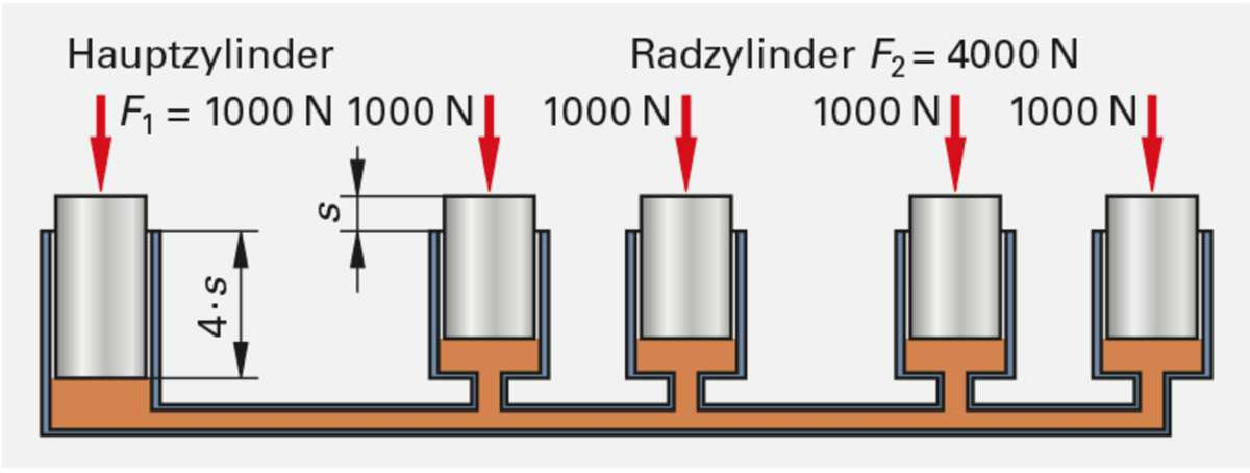
\includegraphics[width=0.5\textwidth]{images/Bremsen/Bremsen-1.pdf}
\caption{hydraulischen Bremse, Quelle: Europa-Verlag}
%\label{fig:}%% anpassen
\end{figure}

\begin{itemize}
\item
  \textbf{geg:}

  \begin{itemize}
  \item
    $p_\text{max} = 180~bar = 1800~N/cm^2, F_\text{Hauptbremszylinder} = 1000~N, F_\text{4x Radzylinder} = 4000~N$,
    $s_\text{Hauptbremszylinder} = 8~mm, s_\text{4x Radzylinder} = 2~mm$
  \end{itemize}
\item
  kleine Kolbenfläche
  $A_\text{Hauptbremszylinder} = \frac{1000~N}{1800~N/cm^2} = 0,55~cm^2$
\item
  große Kolbenfläche
  $A_\text{4x Radzylinder} = \frac{4000~N}{1800~N/cm^2} = 2,22~cm^2$
\item
  übersetzung: 4x Kolbenweg am Hauptbremszylinder
  $i = \frac{2~mm}{8~mm} = 0,25 = 1:4$
\item
  gleiche Arbeit
  $W_\text{Hauptbremszylinder} = 1000~N \cdot 0,008~m = 8~Nm$
\item
  gleiche Arbeit
  $W_\text{4x Radzylinder} = 4000~N \cdot 0,002~m = 8~Nm$
\end{itemize}

\textbf{Nenne Vorteile einer hydraulischen Bremsanlage}

\begin{enumerate}
\item
  Drücke bis 180 bar
\item
  Geringe Flüssigkeitsmengen durch kleine Abmessungen der hydraulischen
  Bremsanlage
\item
  Kleines Lüftspiel
\item
  wartungsarm
\end{enumerate}

\newpage

\section{Bremskraftaufteilung}\label{bremskraftaufteilung}

\textbf{Welche Aufteilung von Bremskreisen gibt es?}

\begin{figure}[!ht]% hier: !ht
\centering
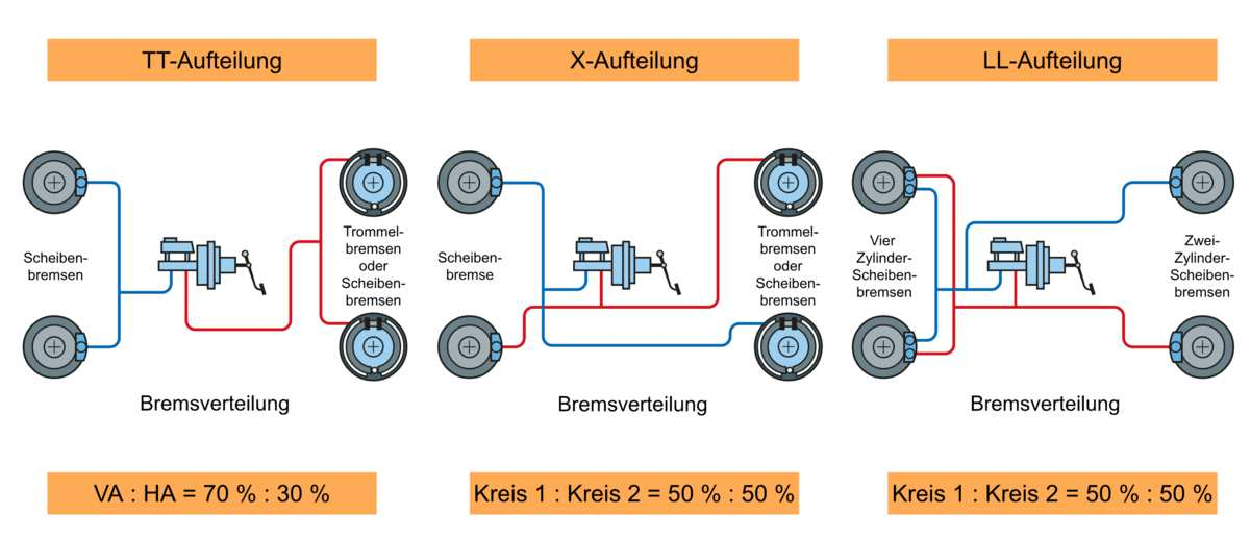
\includegraphics[width=0.5\textwidth]{images/Bremsen/Bremsen-2.pdf}
\caption{Bremskreisaufteilungen, Quelle: Europa-Verlag}
%\label{fig:}%% anpassen
\end{figure}

\begin{enumerate}
\item
  II / TT (Schwarz-weiß) Bremskreis 1 (VA) und Bremskreis 2 (HA)

  \begin{itemize}
  \item
    Bremskraftverteilung VA : HA (70 \% : 30 \%)
  \end{itemize}
\item
  X (Diagonal) Bremskreis 1 (VA links + HA rechts) und Bremskreis 2 (VA
  rechts + HA links)

  \begin{itemize}
  \item
    Bremskraftverteilung Kreis 1 : Kreis 2 (50 \% : 50 \%)
  \end{itemize}
\item
  LL (Dreieck) Bremskreis 1 (VA + HA rechts) und Bremskreis 2 (VA + HA
  links)

  \begin{itemize}
  \item
    Bremskraftverteilung Kreis 1 : Kreis 2 (50 \% : 50 \%)
  \end{itemize}
\end{enumerate}

\textbf{Warum gibt es eine Bremskreisaufteilung?}

Sicheres Abbremsen des Fahrzeugs gewährleisten, bei Ausfall eines
Bremskreises.

\newpage

\section{Hauptbremszylinder}\label{hauptbremszylinder}

\begin{figure}[!ht]% hier: !ht
\centering
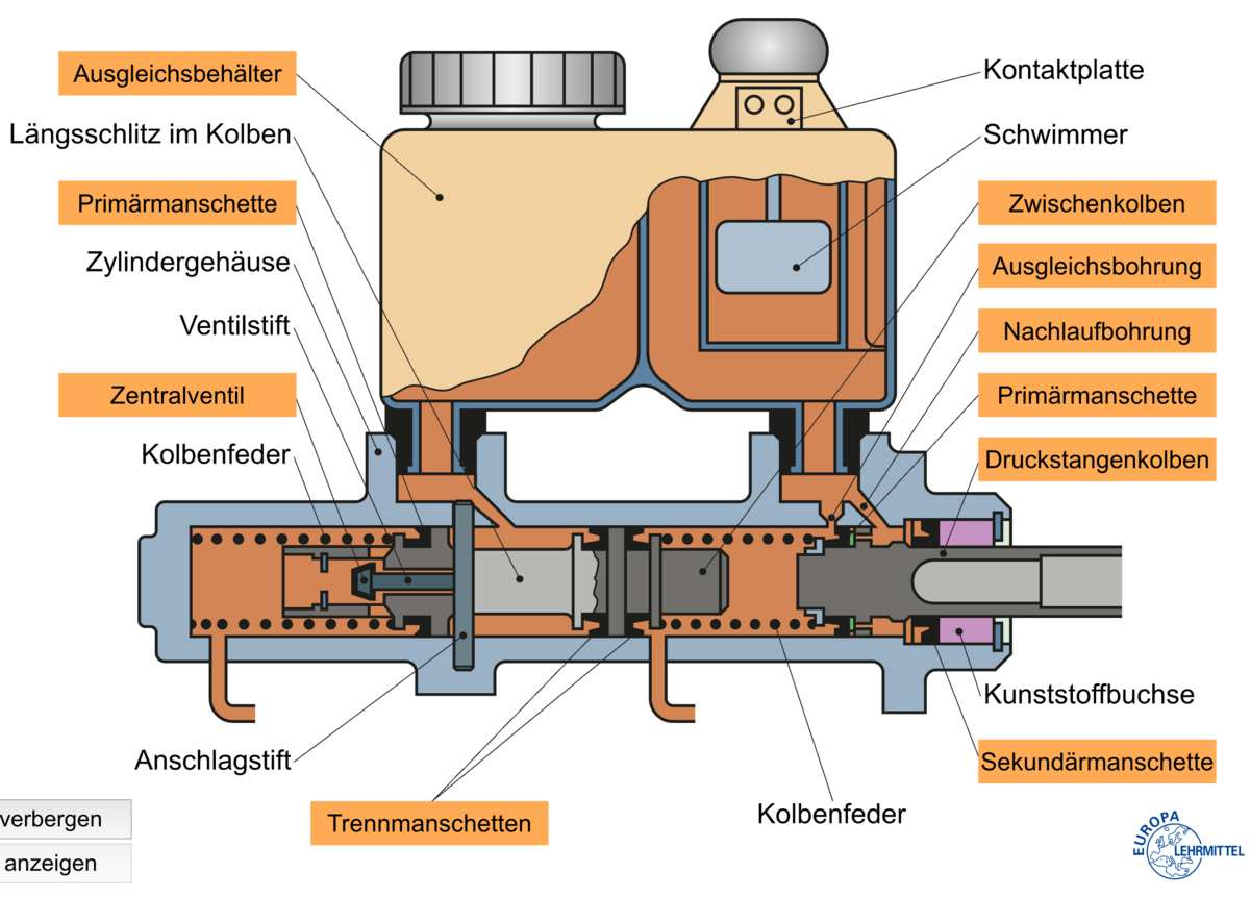
\includegraphics[width=0.5\textwidth]{images/Bremsen/Bremsen-3.pdf}
\caption{Tandem-Hauptbremszylinder, Quelle: Europa-Verlag}
%\label{fig:}%% anpassen
\end{figure}

\textbf{Welche Aufgabe hat der Tandem-Hauptbremszylinder}

\begin{enumerate}
\item
  Umwandeln der Bremskraft in Bremsdruck in der Bremsanlage
\item
  schneller Druckaufbau ermöglichen
\item
  schneller Druckabbau zum Lösen der Bremse
\item
  Absicherung der Bremskreise 1 und 2
\item
  schnelles überwinden der Lüftspiele (Anlegen der Beläge an die
  Scheibe)
\end{enumerate}

\textbf{Primärmanschette} Die Primärmanschette dichtet den Druckraum
beim Bremsvorgang ab, wird beim Schnelllösevorgang als Ventil wirksam
und ermöglicht so das >>Nachsaugen<<.

\textbf{Füllscheibe/Ringscheibe} (Stahl oder Messing) Die Füllscheibe
schützt die Primärmanschette vor Beschädigungen durch die Füllbohrungen
des Kolbens beim Bremsvorgang und wird beim Lösevorgang als Ventil
wirksam.

\textbf{Sekundärmanschette/Ringmanschette} Diese Manschette dichtet den
Ringraum ab. Sie verhindert den Austritt von Flüssigkeit und im
Normalfall auch den Eintritt von Luft

\textbf{Ausgleichsbohrung} ($\varnothing 0,7~mm$) Das
Flüssigkeitsvolumen im Druckraum bei Temperaturschwankungen und beim
Lösevorgang auszugleichen.

\textbf{Nachfüllbohrung} ($\varnothing 3 - 5~mm$) Den Ringraum beim
Lösevorgang auffüllen und einen Lufteintritt in das Bremssystem
verhindern.

\textbf{Zentralventil} verhindert eine Beschädigung der Primärmanschette
des Zwischenkolbenkreises, sobald der dort angeschlossene
Hinterachskreis Blockierneigung aufweist und das ABS dort den
hydraulischen Druck pulsierend regelt.

\textbf{Hochdruckprüfung} 50 -- 100 bar, Prüfdauer 10 Min. (darf max. 10
\% abfallen)

\begin{itemize}
\item
  Undichtigkeit im Bremssystem prüfen
\end{itemize}

\textbf{Niederdruckprüfung} 2 -- 5 bar, Prüfdauer 5 Min. (darf nicht
abfallen)

\begin{itemize}
\item
  Hauptbremszylinder überprüfen

  \begin{itemize}
  \item
    Undichtigkeit am Zentralventil oder an der Primär- oder
    Trennmanschette eines Kolbens
  \end{itemize}
\end{itemize}

\newpage

\section{Trommelbremse}\label{trommelbremse}

\textbf{Nenne Eigenschaften einer Trommelbremse}

\begin{enumerate}
\item
  Selbstverstärkung (Nachteil: keine Dosierbarkeit der Bremskraft)
\item
  Schmutz geschützter Aufbau
\item
  Geringer Bremsbelagverschleiß
\item
  schlechte Wärmeabfuhr
\item
  Neigung zum Fading
\item
  FBA ist einfacher zu integrieren
\end{enumerate}

\textbf{Selbstverstärkung}, die auflaufende Bremsbacke zieht in die
Trommel hinein und verstärkt die Bremswirkung.

\textbf{Bremsfading} Nachlassen der Bremswirkung durch
Temperatureinfluss / Überhitzung. (Bemerkung: Gaspolster entstehen.
Reibzahl des Belags nimmt bei hoher Temperatur ab.)

\textbf{Bremsenkennwert C - Selbstverstärkung} ist abhängig von der
Bauart der Bremse

\textbf{Bauarten einer Trommelbremse}

\begin{figure}[!ht]% hier: !ht
\centering
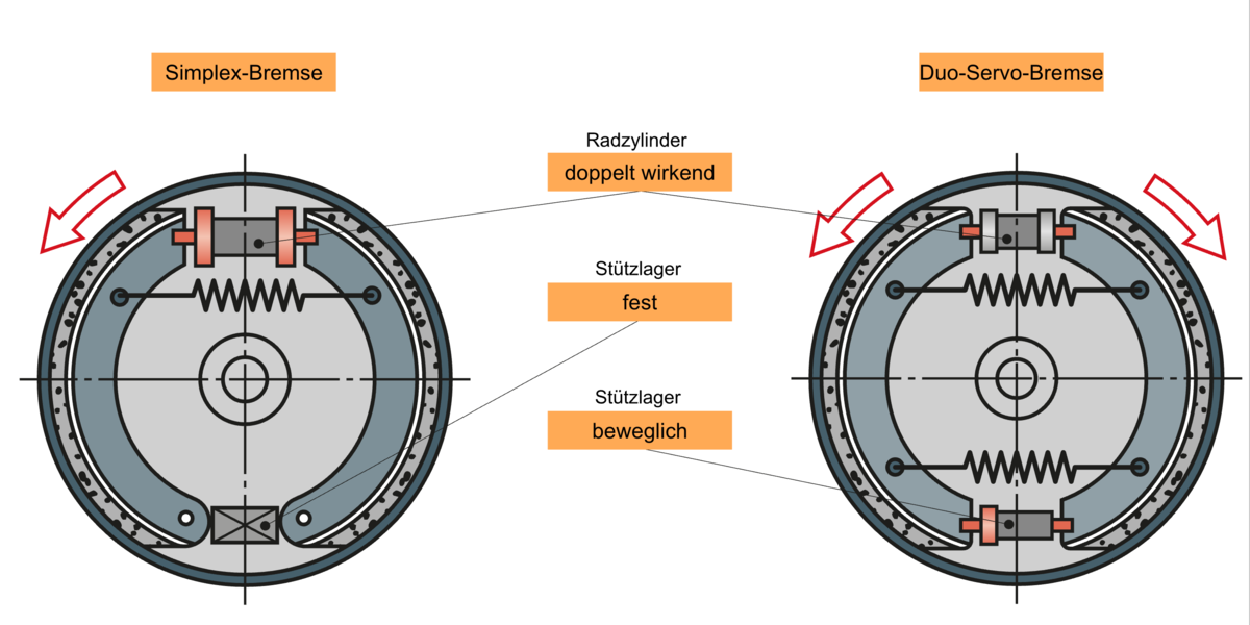
\includegraphics[width=0.5\textwidth]{images/Bremsen/Bremsen-4.pdf}
\caption{Bauarten von Trommelbremsen, Quelle: Europa-Verlag}
%\label{fig:}%% anpassen
\end{figure}

\begin{enumerate}
\item
  \textbf{Duo-Servo-Bremse}

  \begin{itemize}
  \item
    Die untere Abstützung der Bremsbacken nach beiden Seiten beweglich.
  \item
    Es laufen beide Backen bei Vorwärts und Rückwärtsfahrt
    selbstverstärkend auf.
  \end{itemize}
\item
  \textbf{Simplex-Bremse}

  \begin{itemize}
  \item
    Ein Radzylinder mit seinen zwei Kolben betätigt die Bremsbacken.
  \item
    Die Abstützung der Backen erfolgt unten am festen Stützlager.
  \item
    Es gibt bei einer Bremsung in beiden Fahrtrichtungen immer eine
    auflaufende und eine ablaufende Bremsbacke.
  \end{itemize}
\item
  \textbf{Duplex-Bremsen}

  \begin{itemize}
  \item
    Es gibt zwei einseitig wirkende Radzylinder, je Bremsbacke einer.
  \item
    Bei Vorwärtsfahrt wirken beide Bremsbacken auflaufend, also beide
    selbstverstärkend.
  \item
    Bei Rückwärtsfahrt wirken beide Bremsbacken ablaufend, somit ergibt
    sich dann nur eine relativ geringe Bremswirkung.
  \end{itemize}
\end{enumerate}

\textbf{Radbremszylinder} hydraulische Druck wirkt auf einen Kolben und
erzeugt die Spannkraft. Abdichtung durch Nutringmanschette.

\newpage

\section{Scheibenbremse}\label{scheibenbremse}

\textbf{Nenne Eigenschaften einer Schreibenbremse}

\begin{enumerate}
\item
  Verbesserung der Wärmeabfuhr durch innenbelüftete Bremsscheiben
\item
  geringe Neigung zum Fading
\item
  gute Dosierbarkeit der Bremskraft
\item
  höherer Belagverschleiß
\item
  Keine Selbstverstärkung
\item
  gute Kühlung
\item
  Wartung und Belagwechsel einfach
\item
  Selbsttätige Nachstellung des Lüftspiels
\item
  stärkere Erwärmung der Bremsflüssigkeit
\item
  Gefahr der Dampfblasenbildung
\end{enumerate}

\textbf{Bauarten von Scheibenbremsen}

\begin{enumerate}
\item
  \textbf{Festsattel-Scheibenbremse} (mehrere Kolben)
\item
  \textbf{Faustsattel-Scheibenbremse} (ein Kolben)

  \begin{itemize}
  \item
    Geringes Gewicht
  \item
    Kleine Baugröße
  \item
    Gute Wärmeableitung
  \item
    Große Belagflächen
  \item
    Geringer Platzbedarf
  \item
    Geringe Neigung zur Dampfblasenbildung (Bremszylinder ist nur auf
    der Halterseite)
  \item
    Wartungsfreie Gehäuseführung (unempfindlich gegen Schmutz)
  \end{itemize}
\item
  \textbf{Schwimmsattel-Scheibenbremse}
\end{enumerate}

\textbf{Wie erfolgt die Nachstellung bei Scheibenbremsen?
(Kolbenrückstellung)}

\begin{itemize}
\item
  Nach Beendigung des Bremsvorganges und Abbau des Bremsdruckes werden
  die Bremskolben durch das Entspannen des Rechteckringes in ihre
  Ausgangslage gebracht.
\item
  \textbf{Lüftspiel} 0,15 mm.
\item
  Dieser Vorgang kann durch Spreizfedern unterstützt werden.
\end{itemize}

\textbf{Was kann ein Lenkradflattern beim Bremsen verursachen?}

\begin{itemize}
\item
  Radlagerspiel zu groß
\item
  Bremsscheibenschlag zu groß
\end{itemize}

\textbf{Wozu dient eine gelochte oder geschlitzte Bremsscheibe?}

\begin{itemize}
\item
  bei nassen Scheiben schnelle Abfuhr des Wassers
\item
  bessere Kühlung
\item
  bessere Schmutz-, Wasser- und Wärmeabfuhr
\end{itemize}

\textbf{Bremsscheibe}

Die Größe der Bremsscheibe ist ausschlaggebend für das am Rad zur
Verfügung stehende Bremsmoment (ergibt sich aus dem Hebelarm) sowie die
Wärmeabfuhr und Lebensdauer der Scheibe.

Zur besseren Wärmeabfuhr ist sie heutzutage in der Regel innenbelüftet.
Zur besseren Wasser und Schmutzbeseitigung kann sie zudem gelocht oder
geschlitzt sein.

\textbf{Material Kohlefaserverstärkte- oder Keramik-Carbon Bremsscheibe}

\begin{itemize}
\item
  ca. 70 \% leichter
\item
  Hitzebeständigkeit bis zu $1600^\circ\text{C}$ (Vgl. Stahlscheibe
  $800^\circ\text{C}$ Kirschrot)
\item
  nahezu konstanter Reibwert bei Erreichen der Betriebstemperatur
\item
  geringer Verschleiß
\item
  kostenintensiv
\end{itemize}

\textbf{Was bringt es, wenn eine Bremse leichter ist?}

\begin{itemize}
\item
  Weniger \textbf{ungefederte Massen} (alles unterhalb des Stoßdämpfer
  -befestigungspunktes)
\item
  geringere Massenträgheit
\end{itemize}

\textbf{Nenne fünf Anforderungen von Bremsbelägen}

\begin{enumerate}
\item
  Hitzebeständigkeit
\item
  hohe Standzeit
\item
  Wasser und Schmutz unempfindlich
\item
  gleichbleibende hohe Reibungszahl ($\mu$)
\item
  hohe mechanische Festigkeit
\item
  Kein \textbf{Verglasen} (schlechtere Reibungszahl, Scheibe bekommt
  Riefen)
\end{enumerate}

\textbf{Bremsbelag}

\begin{itemize}
\item
  Asbest wurde in Deutschland 1993 verboten und bis 42 \% in Bremsbelag
  enthalten
\item
  mit Prüfzeichen ($E_1$, ECE Genehmigungsnummer) diese belegen, dass
  der Bremsbelag geprüft wurde

  \begin{itemize}
  \item
    gleicher Reibwert wie Original-Beläge des Herstellers
  \item
    Abweichung bis $\pm15 \%$ sind erlaubt
  \item
    Druck- und Scherfestigkeit
  \item
    Asbestfreiheit
  \end{itemize}
\end{itemize}

Eine Prüfnummer mit (E) beginnend, muss am Ersatzteil dauerhaft
identifizierbar vorhanden sein. Die Verpackung der Beläge muss verklebt
oder versiegelt sein, um vorheriges Öffnen klar zu erkennen. Auf der
Verpackung müssen die für den Belag zugelassenen Fahrzeuge gelistet
sein.

\textbf{Arten von Bremskraftverstärkern} (Hilfskraft, Fußkraft des
Fahrers unterstützen)

\begin{enumerate}
\item
  Unterdruck-Bremskraftverstärker

  \begin{itemize}
  \item
    Die geringe \textbf{Druckdifferenz} zwischen Luftdruck 1 bar und
    Saugrohrdruck von etwa 0,2 Bar erfordert große Flächen des
    Arbeitskolbens, um die Druckstangenkraft um den Faktor 4 -- 10 zu
    verstärken.
  \item
    \textbf{Unterdruckerzeugung}

    \begin{itemize}
    \item
      \emph{Dieselmotor:} vom Motor angetriebene Vakuumpumpe
    \item
      \emph{Saug-Ottomotor:} wird dem Ansaugrohr entnommen
    \item
      \emph{Hybridfahrzeug:} Elektrische Vakuumpumpe
    \end{itemize}
  \end{itemize}
\item
  Tandem-Bremskraftverstärker
\item
  Pneumatischer Bremskraftverstärker
\item
  Hydraulischer Bremskraftverstärker
\item
  Elektro-mechanischer Bremskraftverstärker (eBKV, Unterdruck ist nicht
  erforderlich)

  \begin{itemize}
  \item
    Tandem-Hauptbremszylinder mit Vorratsbehälter
  \item
    Elektromotor mit Getriebe und Verstärkungselement
  \item
    Steuergerät
  \item
    Differenzwegsensor
  \end{itemize}
\end{enumerate}

\textbf{Blended Braking} Überlagerung von elektrischem Bremsen
(Rekuperation des Drehstrommotors) + hydraulischem Bremsen = gewünschte
Verzögerung des Fahrers

\textbf{Bremsassistent (BAS)} ab einer bestimmten
Pedalweggeschwindigkeit (Membranwegsensor dient zur Berechnung) wird von
einer Notbremsung ausgegangen, und die Bremsassistentfunktion wird
ausgelöst. Dafür wird im Bremskraftverstärker ein Magnetventil (BAS)
geschaltet, das die Arbeitskammer belüftet und so die maximale
Bremskraftunterstützung gewährleistet. Der Fahrer betätigt das
Bremspedal in einer Gefahrensituation zwar schnell genug, jedoch nicht
stark genug.

\textbf{Feststellbremse}

\begin{enumerate}
\item
  Mechanisch über Bremsseile
\item
  Elektro-mechanische Feststellbremse (Parkbremse, EPB)
\item
  Elektro-mechanischer Aktor
\end{enumerate}

\textbf{Was ist aktive und passive Sicherheit? Nenne jeweils 5x
Beispiele.}

\textbf{Aktive Sicherheit} Maßnahmen zur Vermeidung von Unfällen

\begin{enumerate}
\item
  ABS
\item
  ESP
\item
  Klima
\item
  Scheibenwischer
\item
  ACC (adaptive Geschwindigkeitsregelung)
\item
  Beleuchtungseinrichtung
\item
  Todwinkelassistent
\end{enumerate}

\emph{Klima}: die Raumtemperatur wird runtergekühlt, Aufmerksamkeit
steigt und der Pollenfilter bewirkt eine geringere Last für Allergiker.

\textbf{Passive Sicherheit} Maßnahmen zur Minderung von Unfallfolgen

\begin{enumerate}
\item
  Fahrerairbag
\item
  Beifahrerairbag
\item
  Kopfairbag
\item
  Seitenairbag
\item
  Gurtstraffer
\item
  Batterietrennschalter (Kurzschluss, Brandgefahr)
\item
  Motorhaubenaufsteller
\item
  Nackenstütze
\end{enumerate}

\textbf{Nenne Vorteile und Nachteile einer Scheibenbremse gegenüber
einer Trommelbremse}

\textbf{Vorteile}

\begin{enumerate}
\item
  automatische Nachstellung
\item
  keine Vergrößerung des Bremspedalweges bei erwärmter Bremse
\item
  gleiche Bremswirkung in beiden Fahrrichtungen
\item
  gleiche Bremsbelagbelastung auf einer Achse
\end{enumerate}

\textbf{Nachteile}

\begin{enumerate}
\item
  keine Selbstverstärkung
\item
  starke Erwärmung der Bremsscheiben
\end{enumerate}

\textbf{Welche Siedeanforderung hat DOT4?}

\begin{itemize}
\item
  $\geq 230^\circ\text{C}$
\item
  durch die Wasseraufnahme sinkt der Siedepunkt
\end{itemize}

\chapter{19-Bremsen-II}
%%ju 31-Dez-22 19-Bremsen-II.tex
\section{Grundlagen der
Fahrdynamikregelung}\label{grundlagen-der-fahrdynamikregelung}

\textbf{Kammscher Reibkreis}, die größte auf die Straße übertragbare
Kraft wird als Kreis dargestellt.

Die Kraft, die ein Rad maximal übertragen kann, setzt sich aus der
Aufstandskraft des Rades und der Haftreibung zwischen Reifen und
Fahrbahn zusammen.

\begin{itemize}
\item
  \emph{Innerhalb des Kreises} Kräfte übertragen
\item
  \emph{Außerhalb des Kreises} Schlupf
\item
  $F_\text{max} = F_N \cdot \mu_H$ (Antriebskraft, Bremskraft,
  Normalkraft, Haftreibungszahl)
\item
  $\mu = 0,1$ Eis
\item
  \textbf{stabilen Fahrzustand} Resultierende Kraft aus Umfangskraft und
  Seitenführungskraft muss innerhalb des Kreises liegen
\item
  \textbf{durchdrehende oder blockierende Räder}

  \begin{itemize}
  \item
    Umfangskraft max. und
  \item
    Seitenführungskraft 0
  \item
    Fahrzeug ist nicht mehr lenkbar
  \end{itemize}
\item
  \textbf{max. Kurvengeschwindigkeit}

  \begin{itemize}
  \item
    Seitenführungskraft max.
  \item
    Fahrzeug kann weder gebremst noch beschleunigt werden (würde
    ausbrechen)
  \end{itemize}
\end{itemize}

\textbf{Schlupf}

Das Verhältnis der Fahrgeschwindigkeit zu Radumfangsgeschwindigkeit oder
das Verhältnis der tatsächlich zurückgelegten Wegstrecke zum dynamischen
Abholumfang. (blockiert ein Rad, dann ist der Schlupf 100 \%)

\textbf{dynamischen Abrollumfang}

\begin{itemize}
\item
  Reifenaufstandsfläche = Latsch
\item
  Wenn sich das Rad dreht, verändert sich der Reifenumfang, als wenn das
  Fahrzeug steht.
\item
  Verlängerung des Weges durch Schlupf oder Verformung des Reifens.
\end{itemize}

\textbf{Typgenehmigung} für ABS nein und ESP ja

\section{ABS}\label{abs}

\textbf{ABS-Arbeitsbereich}

\textbf{stabilen Bereich}, um ein ausreichendes Maß an
Seitenführungskraft bereitstellen zu können. Zwischen 8 -- 35 \%
Schlupf.

\textbf{ABS-Aufgaben}

\begin{itemize}
\item
  Erhalt der Seitenführungskraft durch Begrenzung der maximalen
  Bremskraft
\item
  Vermeidung von Bremsplatten
\end{itemize}

\textbf{Maximale Bremskraft} Übergang von Haftreibung zur Gleitreibung

\textbf{ABS-Funktion}

\begin{itemize}
\item
  Erfassen der Raddrehzahlsignale, die miteinander verglichen werden
\item
  weicht ein Rad ab und bei kritischen Schlupfwerten
\item
  wird die Bremskraft begrenzt durch \textbf{3x Regelphasen}
\item
  Regelzyklus 4 -- 10x pro Sekunde (10 Hz)
\end{itemize}

\begin{enumerate}
\item
  \textbf{Druck halten}

  \begin{itemize}
  \item
    Einlassventil wird geschlossen und Druck an Radbremse konstant
    gehalten.
  \end{itemize}
\item
  \textbf{Druck ablassen}

  \begin{itemize}
  \item
    Auslassventil wird geöffnet und Bremsdruck wird gesandt.
  \end{itemize}
\item
  \textbf{Druck aufbau}

  \begin{itemize}
  \item
    Sinkt der Schlupf auf unkritischer Werte, öffnet das Einlassventil
    und wird mit maximaler Bremskraft verzögern.
  \end{itemize}
\end{enumerate}

\textbf{Regelungsarten des ABS}

\begin{enumerate}
\item
  \textbf{Select-Low-Regelung} (HA)

  \begin{itemize}
  \item
    Das Rad mit der geringeren Bodenhaftung bestimmt den gemeinsamen
    Bremsdruck einer Achse.
  \end{itemize}
\item
  \textbf{Individualregelung} (VA)

  \begin{itemize}
  \item
    wird jedem Rad die maximale übertragbare Bremskraft zugeteilt.
  \item
    Unterschiedliche Bremskräfte wirken.

    \begin{itemize}
    \item
      Ein Giermoment entsteht in Richtung des Rades mit der größeren
      Haftung. Kann durch Gegenlenken, ausgeglichen werden. (Vgl.
      Negativer Lenkrollradius)
    \end{itemize}
  \end{itemize}
\end{enumerate}

\textbf{Negativer Lenkrollradius} (Lenkrollhalbmesser) an Vorderachse

Erzeugt ein automatisches Gegenlenken, d.h. der Reifen schwenkt nach
innen an der Vorderachse.

\textbf{ABS-Sensoren}

\begin{itemize}
\item
  Geschwindigkeit von ca. 6 km/h notwendig
\item
  Induktiv-Sensor (Bosch: passiv)

  \begin{itemize}
  \item
    Spule und Magnetfeld $\to$ Wechselspannung
  \end{itemize}
\item
  Hall-Sensor (Bosch: aktiv)

  \begin{itemize}
  \item
    eigene Spannungsversorgung
  \item
    Kabel kann 2-adrig sein (Masseleitung = Signalleitung)
  \item
    Stromsignal an SG
  \item
    Prüfen: Strommessung
  \end{itemize}
\end{itemize}

\textbf{Regelkanäle von ABS}

\begin{enumerate}
\item
  2 Kanal ABS-System (VA und HA)
\item
  3 Kanal ABS-System (VA rechts + links und HA)
\item
  4 Kanal ABS-System (4S4M, Sensoren und Modulatoren)
\end{enumerate}

\section{ASR}\label{asr}

Erfassung des Radschlupfs an den Antriebsrädern durch Abgleichen der
Drehzahlsignale. Bei kritischen Schlupfwerten begrenzen der
Antriebskraft durch Verringern des Motordrehmoments oder Bremseingriff.

\section{FDR / ESP}\label{fdr-esp}

Fahrdynamische Prozesse erfassen und autonom regeln.

\textbf{Systeme}

\begin{enumerate}
\item
  (+) Antiblockiersystem (ABS)
\item
  (+) Elektronische Bremskraftverteilung (EBV)
\item
  (+) Antriebsschlupfregelung (ASR) mit Motorschleppmoment-Regelung
  (MSR)
\item
  (+) Giermomentregelung (GMR)
\item
  (=) Fahrdynamikregelsystem (FDR) = Elektronisches Stabilitätsprogramm
  (ESP)
\end{enumerate}

\textbf{Komponenten}

\begin{enumerate}
\item
  Hydraulikeinheit
\item
  Lenkwinkelsensor
\item
  Tandem-Hauptzylinder mit Drucksensoren
\item
  Querbeschleunigungs- und Gierratensensor
\item
  Raddrehzahlsensor
\item
  Motormanagement
\end{enumerate}

\textbf{Gierratenerfassung}

Erfassen der Drehbewegung des Fahrzeugs um seine eigene Hochachse
mithilfe der Corioliskraft (Piezo-Element wird gestaucht oder gestreckt
$\to$ SG).

\textbf{Bewegungen und Kräfte des Fahrzeugs}

\begin{enumerate}
\item
  Hochachse - Gieren (Schleudern, Drehbewegung)

  \begin{itemize}
  \item
    Radlast, Kräfte durch Fahrbahnunebenheiten
  \end{itemize}
\item
  Längsachse - Wanken (Kippbewegung)

  \begin{itemize}
  \item
    Antriebskraft, Bremskraft, Reibungskraft
  \end{itemize}
\item
  Querachse - Nicken (Drehbewegung)

  \begin{itemize}
  \item
    Fliehkraft, Seitenwindkraft, Seitenführungskraft
  \end{itemize}
\end{enumerate}

\chapter{19-Loesung-Bremse-I}
%%ju 31-Dez-22 19-Loesung-Bremse-I.tex
\textbf{1) Erläutern Sie den Begriff Nass -- Siedepunkt.}

Nass-Siedepunkt ist der Siedepunkt bei 3,5 \% Wasseranteil.

\textbf{2) Beschreiben Sie den Druckaufbau in einem Tandem --
Hauptzylinder.}

\textbf{Druckaufbau}, bei Bremsbetätigung bewegen sich der
Druckstangenkolben und der Zwischenkolben und überfahren die
Ausgleichsbohrungen und drücken Bremsflüssigkeit über die
Druckanschlüsse in die Bremskreise. Mit steigendem Druck wird der
Zwischenkolben nicht mehr von der gefesselten Kolbenfeder, sondern vom
Druck der Bremsflüssigkeit bewegt.

Der Fahrer betätigt mithilfe des Bremspedals und der Unterstützung eines
Bremskraftverstärkers den Druckstangenkolben. Die Primärmanschette
überfährt die Ausgleichsbohrung, wodurch der erste Bremskreis druckdicht
abgeschlossen ist. Durch weiteres Betätigen verdrängt der
Druckstangenkolben die hinter ihm befindliche Flüssigkeit, wodurch sich
der Zwischenkolben verschiebt. Dessen Primärmanschette überfährt die
Ausgleichsbohrung des zweiten Bremskreises, sodass dieser ebenfalls
druckdicht abgeschlossen ist. Jede weitere Betätigung Druckstangenkolben
führt zu einem gleichmäßigen Druckaufbau in beiden Bremskreisen.

\textbf{3) Beschreiben Sie, wie ein Tandem -- Hauptzylinder arbeitet,
wenn der Druckstangenkolbenkreis ausfällt.}

Der Druckstangenkolben durchfährt den undichten Druckraum des ersten
Bremskreises und läuft mechanisch auf dem Zwischenkolben auf. Wird der
Druckstangenkolben weiter verschoben, verschiebt dieser den
Zwischenkolben, wodurch im zweiten Bremskreis Bremsdruck aufgebaut wird.
Längerer Pedalweg.

\textbf{4) Beschreiben Sie den Füllvorgang bei einem Hauptzylinder mit
Zentralventil, Primärmanschette und Füllscheibe.}

Wird das Bremspedsal losgelassen, so werden Druckstangenkolben und
Zwischenkolben durch die Kolbenfedern in ihre Ausgangslage
zurückgeschoben. Ist es durch den Verschleiß von Bremsbelag oder
Bremsscheibe während des Bremsvorganges zu einem Flüssigkeitsverlust
gekommen, so muss dieser ausgeglichen werden. Dies geschieht im ersten
Bremskreis durch Abklappen der Primärmanschette vom Druckstangenkolben.
Die Füllscheibe hebt sich ab und die Nachlaufbohrungen werden frei.
Hierdurch kann Bremsflüssigkeit an der Füllscheibe und der
Primamanschette vorbei nachfließen. Im zweiten Bremskreis geschieht dies
durch Öffnen des Zentralventils, welche so verbaut ist, dass ein
Nachfließen von Bremsflüssigkeit in den Bremskreis jederzeit möglich
ist.

\textbf{5) Beschreiben Sie die Funktionsweise des gestuften
Tandem--Hauptzylinders bei intakten Bremskreisen und bei Ausfall eines
Bremskreises.}

Bemerkung: TT - Bremskreisaufteilung (schwarz-weiß), die
Zylinderdurchmesser sind gestuft. (Druckstangenkolben $\to$ VA-Kreis,
Zwischenkolben $\to$ HA-Kreis), Ausfall VA-Kreises: über HA 30 \%
Bremswirkung, Ausfall HA-Kreises: über VA 70 \% Bremswirkung

\begin{itemize}
\item
  \textbf{intakten Bremskreisen}

  \begin{itemize}
  \item
    Vorteil gegenüber normalen HBZ: ist in der Verdrängung eines
    größeren Flüssigkeitsvolumens im ersten Bremskreis, was zu einem
    schnelleren Ansprechen der vorderen Radbremsen führt.
  \end{itemize}
\item
  \textbf{Ausfall des vorderen Bremskreises}

  \begin{itemize}
  \item
    läuft der Druckstangenkolben direkt auf den Zwischenkolben auf. Da
    dieser eine kleinere Kolbenfläche hat, als der Druckstangenkolben
    kommt es bei gleicher Pedalkraft zu einer Druckerhöhung im hinteren
    Bremskreis.
  \end{itemize}
\item
  \textbf{Ausfall des hinteren Bremskreises}

  \begin{itemize}
  \item
    wird der Zwischenkolben bis an das Gehäuse des Hauptbremszylinders
    geschoben. Es kommt zu einem Druckaufbau im vorderen Bremskreis. Am
    Bremsdruck ändert sich in diesem Fall nichts, da die wirksame
    Kolbenfläche die gleiche ist, wie bei intakten Bremskreisen.
  \end{itemize}
\end{itemize}

\textbf{6) Welche Fehler lassen sich bei einer Niederdruckprüfung an
einer hydraulischen Bremsanlage feststellen?}

\begin{itemize}
\item
  Undichtigkeiten der Dichtungen innerhalb des Hauptbremszylinders
\item
  Undichtigkeiten der Bremsanlage nach außen
\end{itemize}

\textbf{7) Beschreiben Sie, wie im Bremskraftverstärker eine
Teilbremsung gesteuert wird.}

Sobald das Bremspedal betätigt wird, verschiebt sich der, am Ende der
Kolbenstange befindliche Ventilkolben und schließt zunächst das
Trennventil. Unterdruck und Arbeitskammer sind voneinander getrennt.
Durch weiteres betätigen der Kolbenstange wird der Ventilkolben in eine
Reaktionscheibe gepresst und das Außenluftventil öffnet. Der
Arbeitskolben verschiebt sich und unterstützt die Fußkraft des Fahrers
an der Kolbenstange des Hauptbremszylinders. Hält der Fahrer die
Position des Bremspedals konstant, um eine Teilbremsung zu erreichen, so
verschiebt sich der Arbeitskolben noch so lange weiter, bis das
Außenluftventil wieder geschlossen ist. Da das Trennventil bis zum
Loslassen des Pedals ebenfalls geschlossen bleibt, gerät der
Bremskraftverstärker in eine Ruhelage und hält die Position.

\textbf{8) Erläutern Sie den Begriff Bremsenkennwert >>C<<.}

Faktor der Selbstverstärkung einer Trommelbremse

\textbf{9) Beschreiben Sie, wie das Lüftspiel zwischen Bremsbelag und
Scheibe entsteht und wie groß es i.d.R. ist.}

\begin{itemize}
\item
  Die Abdichtung zwischen Bremskolben und Gehäuse erfolgt bei der
  Scheibenbremse mittels eines Rechteckringes.
\item
  Wird die Bremse betätigt, so haftet dieser Rechteckring am
  Bremskolben, wodurch sich der Rechteckring verspannt.
\item
  Wird die Bremse gelöst, entspannt sich der Rechteckring wieder und
  >>zieht<< den Bremskolben zurück.
\item
  Der Vorgang kann durch eine Spreizfeder zwischen den Belägen
  unterstützt werden.
\item
  Lüftspiel ca. 0,15 mm.
\end{itemize}

\textbf{10) Erläutern Sie den Unterschied zwischen Bremsdruckreglern und
lastabhängigen Bremsdruckbegrenzern.}

\begin{itemize}
\item
  \textbf{Bremsdruckregler}

  \begin{itemize}
  \item
    Sorgen dafür, dass der Bremsdruck an der Hinterachse, und
    Bremsvorgängen nur noch verwendet Anstalt. Hiermit wird der
    dynamischen Achslastverlagerung Rechnung getragen.
  \end{itemize}
\item
  \textbf{lastabhängige Bremskraftbegrenzer}

  \begin{itemize}
  \item
    Begrenzen den Bremsdruck an der Hinterachse auf einen definierten
    Wert. Die Höhe des maximalen Bremsdruckes ist von der Beladung des
    Fahrzeuges abhängig und wird durch die Änderung der
    Federvorspannkraft des Begrenzers festgelegt.
  \end{itemize}
\end{itemize}

\chapter{19-Loesung-Bremse-II}
%%ju 31-Dez-22 19-Loesung-Bremse-II.tex
\textbf{1) Was versteht man unter Schlupf?}

Schlupf ist die Differenz zwischen der Fahrgeschwindigkeit und der
Radumfangsgeschwindigkeit.

\textbf{2) Was geschieht während der ABS -- Regelung?}

\begin{itemize}
\item
  Zunächst wird der Druckaufbau gestoppt
\item
  Wenn der Schlupf weiter zunimmt, wird der Druck geringfügig gesenkt
\item
  Wenn der Schlupf wieder abnimmt, wird der Druck erhöht, um im
  optimalen Bremsbereich zu bleiben
\end{itemize}

Bemerkung:

Das ABS-Steuergerät erhält zur Regelung des Bremsvorgangs die
Radgeschwindigkeit von den Raddrehzahlsensoren.

\begin{itemize}
\item
  sinusförmige Wechselspannung (Induktivgeber)
\item
  oder ein Rechtecksignal (Hallgeber)
\end{itemize}

Daraus wird eine Fahrzeug-Referenzgeschwindigkeit gebildet. Das
Steuergerät erkennt Drehzahländerungen an einem oder mehreren Rädern.

Sinkt die Raddrehzahl innerhalb einer Zeitspanne oder in Bezug auf die
Referenzgeschwindigkeit, wird das als Blockiergefahr erkannt.

\textbf{3) Wie viele ABS -- Regelkreise können bei einem Fahrzeug mit
hydraulischer Bremsanlage vorhanden sein? Wie sind diese ggf.
zugeordnet?}

\begin{itemize}
\item
  2 $\to$ je ein Regelkreis pro Vorderrad
\item
  3 $\to$ je ein Regelkreis für jedes Rad der Vorderachse und ein
  gemeinsamer Regelkreis für die Räder der Hinterachse.
\item
  4 $\to$ je ein Regelkreis für jedes Rad der Vorder- und Hinterachse
\end{itemize}

\textbf{4) Wie ist ein aktiver Drehzahlsensor aufgebaut?}

Der Hall-Sensor besteht im Wesentlichen aus einem stromdurchflossen,
Halbleiterbauelement und einem magnetischen, in Nord- und Südpole
unterteilten Impulsring. Ändert sich die Polarität des, auf das
Hall-Element wirkenden Magnetfeldes, ändert sich die Hallspannung
innerhalb des Halbleiters, woraus die integrierte Auswerteelektronik ein
Rechtecksignal formt und dieses an das Steuergerät sendet. Die Frequenz
des Rechteckssignals ist proportional zur Raddrehzahl.

\textbf{5) Warum lässt sich ein Fahrzeug bei Ausfall des ABS noch normal
bremsen?}

In der Ruhelage sind die Magnetventile in der Hydraulikeinheit
einlassseitig geöffnet und auslassseitig geschlossen.

\textbf{6) Wie ist die grundsätzliche Wirkungsweise der
Antriebsschlupfregelung (ASR)?}

Wird an einem der Antriebsräder ein erhöhter Schlupf (> 8
-- 35 \%) erkannt, so wird systemabhängig das Motordrehmoment reduziert
und/oder die durchdrehenden Rad/Räder mithilfe der Betriebsbremse
abgebremst.

\textbf{7) Was wird durch die Motorschleppmomentregelung (MSR)
verhindert?}

Verhindert durch automatische Erhöhung des Motormoments, dass die
Antriebsräder aufgrund der Abbremsung durch den Motor bei plötzlicher
Gaswegnahme oder beim Zurückschalten einen erhöhten Schlupf aufweisen.

\textbf{8) Was versteht man unter dem Begriff >>Giermoment<<?}

\textbf{Giermoment / Drehrate} Drehung des Fahrzeugs um die
Fahrzeughochachse

\textbf{9) Welche Systeme bilden mit ihren Funktionen das eigentliche
elektronische Stabilitätsprogramm (ESP)?}

\begin{enumerate}
\item
  (+) Antiblockiersystem (ABS)
\item
  (+) Elektronische Bremskraftverteilung (EBV)
\item
  (+) Antriebsschlupfregelung (ASR)
\item
  (+) Motorschleppmomentregelung (MSR)
\item
  (+) Giermomentregelung (GMR)
\item
  (=) Fahrdynamikregelsystem (FDR) = Elektronisches Stabilitätsprogramm
  (ESP)
\end{enumerate}

\textbf{10) Wie reagiert das ESP -- Steuergerät beim Übersteuern eines
Fahrzeugs mit Standardantrieb?}

\textbf{ESP-Eingriff beim Übersteuern:}

\begin{itemize}
\item
  \emph{ohne ESP} würde beim Fahrzeug das Heck ausbrechen und der Fahrer
  muss gegenlenken.
\item
  \emph{mit ESP} unterstützt den Fahrer durch einen Bremseingriff,
  vorwiegend am kurvenäußeren Vorderrad. Dadurch entsteht ein
  Giermoment/Drehrate um die Hochachse, das das Auto wieder auf den
  gewünschten Fahrkurs zieht.
\item
  Das Antriebsmoment der Hinterräder gesenkt und deren
  Seitenführungskräfte zu erhöhen
\end{itemize}

Bemerkung:

\textbf{ESP-Eingriff beim Untersteuern:}

\begin{itemize}
\item
  \emph{ohne ESP} würde das Fahrzeug über die Vorderräder aus der Kurve
  schieben.
\item
  \emph{mit ESP} unterstützt die Lenkkorrektur des Fahrers durch einen
  Bremseingriff, vorwiegend am kurveninneren Hinterrad. Dadurch entsteht
  ein Giermoment/Drehrate um die Hochachse, das das Auto in die Kurve
  hineindreht.
\end{itemize}

\chapter{19-Loesung-Bremse-III}
%%ju 31-Dez-22 19-Loesung-Bremse-III.tex
\textbf{1) Was versteht man unter der Bezeichnung >>Betriebsbremse<<
eines Fahrzeuges?}

Ermöglicht dem Fahrzeugführer mit abstufbarer Wirkung, die
Geschwindigkeit eines Fahrzeuges während seines Betriebs zu verringern
oder zum Stillstand zu bringen und zu halten.

\textbf{2) Welche Bremswirkung muss die Dauerbremse haben?}

Die Dauerbremse muss das Fahrzeug in einem niedrigen Gang gemäß
Herstellerangaben, in einem Gefälle von 7 \% und einer Länge von 6 km
auf 30 km/h halten können.

\textbf{3) Erklären Sie die Bezeichnung >>2--Leitungs--Bremsanlage<<.}

Bei der 2-Leitungs-Bremsanlage besteht eine Verbindung der Bremsanlage
vom Motorwagen zu der Bremsanlage des Anhängers durch zwei
Druckluftleitungen. Eine davon dient als Vorratsleitung zur Übertragung
der Vorratsluft, die andere als Bremsleitung zur Übertragung der
Steuerdrücke.

\textbf{4) Was versteht man unter dem >>Elektronischen Bremssystem<<
(EBS) bei der Druckluftbremse?}

Es ist eine Kombination aus einer 2-Kreis-Druckluftbremsanlage mit
Antiblockiersystem (ABS) und Antriebsschlupfregelung (ASR) und
zusätzlich einer elektronischen Steuerung zur schnellen Ansteuerung der
Radbremsen.

\begin{itemize}
\item
  Schnellere Ansprechzeiten
\item
  Kürzere Bremswege
\item
  Geringerer Verschleiß
\item
  verbesserte Lastzugabstimmung
\end{itemize}

\textbf{5) Welche Aufgabe hat die automatische Frostschutzpumpe?}

Die automatische Frostschutzpumpe soll bei Temperaturen um den
Gefrierpunkt und darunter pro Schaltimpuls des Druckreglers ca.
$0,6~cm^3$ Frostschutzmittel in das Leitungssystem der Druckluftanlage
einspritzen.

\textbf{6) Wie wird der Lufttrockner regeneriert?}

\textbf{Einkammer-Lufttrockner}

In der Füllphase wird ein Teil der geförderten Luft in einem
Regenerationsbehälter gespeichert. Mit dem Abschaltimpuls des
Druckregelers wird diese Luft in entgegengesetzte Richtung durch den
Lufttrockner geblasen, wodurch das Granulat getrocknet wird.

\textbf{Zweikammer-Lufttrockner}

In der Füllphase kommt nur eine Trocknerpatrone zum Einsatz. Die zweite
Patrone wird in diese Zeit durch einen Teil der getrockneten Luft aus
der ersten Patrone regeneriert. Alle 60 Sekunden wird zwischen den
beiden Trocknerpatronen umgeschaltet.

\textbf{7) Welche Aufgaben hat das >>4 -- Kreis -- Schutzventil<<?}

\begin{itemize}
\item
  Verteilung der Druckluft auf die einzelnen Bremskreise
\item
  Vorrangige Befüllung der Betriebsbremskreise
\item
  Drucksicherung in den übrigen Bremskreisen bei Druckabfall in einem
  Bremskreis
\item
  Anfahrsperre bei Druckverlust auf Bremskreis 1 (Bleed-Back)
\end{itemize}

\textbf{8) Wozu benötigt man die Kontrollstellung am Handbremsventil?}

Durch die Kontrollstellung kann der Fahrer feststellen, ob sein in
Hanglage abgestellter Lastzug auch dann noch gesichert bleibt, wenn sich
die Bremse des Anhängers infolge von Druckverlust löst.

\textbf{9) Warum ist eine Lastzugabstimmung erforderlich?}

Die Lastzugabstimmung gewährleistet, dass der ziehende Motorwagen und
der gezogene Anhänger oder Auflieger bei allen Bremsdrücken und
Lastzuständen ein etwa gleichmäßiges Bremsverhalten und einen etwa
gleichmäßigen Bremsbelagverschleiß haben.

\textbf{10) Was passiert bei Abriss der gelben Bremsleitung?}

\begin{itemize}
\item
  \textbf{Abriss der Bremsleitung} (Gelb)

  \begin{itemize}
  \item
    Zunächst bleiben die Bremsen gelöst. Beim Betätigen einer Bremse
    entweicht Luft am Anhängersteuerventil, wodurch dieses eine
    Vollbremsung im Anhänger auslöst. Nach dem Lösen der Bremse im
    Motorwagen wird auch die Anhängerbremse wieder frei.
  \end{itemize}
\end{itemize}

Bemerkung:

\textbf{Abriss der Vorratsleitung} (Rot) Anhänger muss automatisch
Bremsen

\chapter{20-Fahrwerk}
%%ju 31-Dez-22 20-Fahrwerk.tex
BEMERKUNG: Vgl. handschriftliche Notizen

\chapter{20-Loesung-Fahrwerk}
%%ju 26-Dez-22 20-Loesung-Fahrwerk.tex
\textbf{1. Was wird als Radsturz bezeichnet?}

\begin{itemize}
\item
  Als Radsturz bezeichnet man die Neigung der Radebene gegenüber einer
  gedachten, senkrecht zur Fahrbahn verlaufenden Ebene

  \begin{itemize}
  \item
    Radstellung geradeaus
  \item
    Blick parallel zur Fahrzeuglängsachse
  \end{itemize}
\end{itemize}

\textbf{2. Was ist ein >>Negativer Lenkrollhalbmesser<<? Welchen
Einfluss hat er auf das Fahrverhalten des Fahrzeugs?}

\begin{itemize}
\item
  Vom negativen Lenkrollhalbmesser spricht man, wenn sich die
  Mittellinien durch das Rad und durch die Spreizachse schon oberhalb
  der Fahrbahn schneiden.
\item
  Durch den negativen Lenkrollhalbmesser wird eine Selbststabilisierung
  des Fahrzeugs erreicht. Das bedeutet, der Fahrer braucht keine
  Kurskorrektur durchzuführen, wenn

  \begin{itemize}
  \item
    beim Bremsen die Bodenhaftung unterschiedlich ist
  \item
    die Bremswirkung an den Rädern unterschiedlich ist
  \item
    die Räder stark unterschiedlichen Reifendruck haben
  \end{itemize}
\end{itemize}

\textbf{3. Was versteht man beim Kfz als Übersteuern?}

\begin{itemize}
\item
  Beim Übersteuern drängt das Fahrzeug bei schneller Kurvenfahrt mit den
  Hinterrädern nach außen. Der Schräglaufwinkel der Hinterräder ist
  größer als der Schräglaufwinkel der Vorderräder.
\item
  Das Fahrzeug durchfährt einen kleineren Kurvenradius, als es der
  Lenkeinschlag vorgibt. Um der Kurve weiter zu folgen, muss
  gegengelenkt werden.
\end{itemize}

\textbf{4. Was zählt beim Kfz zu den ungefederten Massen?}

\begin{itemize}
\item
  Alle Bauteile unterhalb der Fahrzeugfederung, wie zum Beispiel Rad und
  Reifen, Radnabe, Bremsen und Achsschenkel.
\end{itemize}

\textbf{5. Welche Vor- und Nachteile hat eine Starrachse?}

\textbf{Vorteile}

\begin{itemize}
\item
  hohe statische Belastbarkeit
\item
  keine Änderung von Sturz, Spreizung und Spur beim Ein- und Ausfedern
\end{itemize}

\textbf{Nachteile}

\begin{itemize}
\item
  Hohes Gewicht und dadurch große ungefederte Masse
\end{itemize}

\textbf{6. Welche Aufgabe hat der Panhardstab?}

\begin{itemize}
\item
  Er dient zur seitlichen Führung der Karosserie auf der Hinterachse.
\end{itemize}

\textbf{7. Was erreicht man mit einer Raum-Lenker-Hinterachse?}

\begin{itemize}
\item
  Man erreicht mit bis zu 5 Lenkern pro Rad eine exakte Radführung, und
  eine geringfügige Änderung von Sturz und Spur beim Ein- und Ausfedern,
  Beschleunigen und Bremsen
\end{itemize}

\chapter{21-Loesung-Federung}
%%ju 31-Dez-22 21-Loesung-Federung.tex
\textbf{1. Welche Aufgaben muss die Federung im Kfz übernehmen?}

\begin{itemize}
\item
  Sie soll die Stöße, die durch Fahrbahnunebenheiten auf die Karosserie
  einwirken, in Schwingungen umwandeln
\end{itemize}

Dies verbessert

\begin{itemize}
\item
  den Fahrkomfort für die Insassen
\item
  den Schutz des Ladegutes
\item
  die Bodenhaftung zur Erhöhung der Fahrsicherheit
\end{itemize}

\textbf{2. Welche Vorteile haben Schraubenfedern gegenüber Blattfedern?}

\begin{itemize}
\item
  Geringes Gewicht
\item
  Geringerer Bauraumbedarf
\item
  Reibungsarm

  \begin{itemize}
  \item
    Geringe Eigendämpfung

    \begin{itemize}
    \item
      Dämpfungsrate wird überwiegend durch Schwingungsdämpfung bestimmt
      und ist somit besser einstellbar
    \end{itemize}
  \item
    Wartungsfrei
  \end{itemize}
\item
  Auslegung linear und progressiv möglich
\item
  Kopplung mit der >>Active Body Control<< möglich
\end{itemize}

\textbf{3. Wie erreicht man bei Schraubenfedern eine progressive
Kennlinie?}

\begin{itemize}
\item
  Eine progressive Kennlinie, d.h. eine zunehmende Federhärte mit
  zunehmendem Federweg, erreicht man bei der Schraubenfeder durch
  unterschiedliche Windungsdurchmesser (taillierte Feder, Tonnenfeder,
  Minibloc-Feder) oder durch unterschiedliche Drahtdurchmesser in den
  einzelnen Windungen
\end{itemize}

\textbf{4. Welche Vorteile bietet die Luftfederung?}

\begin{itemize}
\item
  Gleichbleibend hoher Federungskomfort
\item
  Fahrzeugniveau unabhängig von Beladungszustand
\item
  Spur und Sturz bleiben unverändert
\item
  Fahrzeugniveau situationsabhängig adaptierbar

  \begin{itemize}
  \item
    Senkung bei Hochgeschwindigkeit
  \item
    Anhebung bei Schlechtwegfahrten
  \item
    Höhenanpassung bei Einstieg und Beladung
  \item
    Dynamischer Nick-- und Wankausgleich
  \end{itemize}
\item
  Keine >>trampelnden<< Achsen bei Leerfahrten
\item
  Kopplung mit Druckluftbremse möglich
\end{itemize}

\textbf{5. Wie ist die grundsätzliche Wirkungsweise der
hydropneumatischen Federung?}

\begin{itemize}
\item
  Beim Einfedern wird die Bewegung der Räder über einen Kolben auf ein
  Ölvolumen übertragen, welches sich wiederum auf ein Gaspolster
  abstützt.
\end{itemize}

\textbf{6. Welche Aufgaben erfüllen Stoßdämpfer am Kfz?}

\begin{itemize}
\item
  Die Stoßdämpfer wandeln die Schwingungen der Federung durch Reibung in
  Wärme um, um die Anzahl der Amplituden nach einem Fahrbahnstoß zu
  reduzieren

  \begin{itemize}
  \item
    Verbesserung der Fahrsicherheit durch gleichbleibend guten
    Bodenkontakt
  \item
    Erhöhung des Fahrtkomforts
  \end{itemize}
\end{itemize}

\textbf{7. Welcher Unterschied besteht zwischen}

\begin{itemize}
\item
  \textbf{a) dem Zweirohr-Stoßdämpfer und}
\item
  \textbf{b) dem Einrohr-Gasdruck-Stoßdämpfer?}
\end{itemize}

\begin{enumerate}
\def\labelenumi{\alph{enumi})}
\item
  Der Zweirohr-Stoßdämpfer besitzt zur Aufnahme des
  Kolbenstangenvolumens bei Einfedern einen Vorratsraum, der rund um den
  eigentlichen Arbeitsraum angeordnet ist. Dieser wirkt isolieren,
  wodurch die, im Arbeitsraum entstehende Wärmemenge nur schlecht
  abgeführt werden kann. Hierdurch hat der Dämpfer eine hohe Tendenz zur
  Ölverschäumung, die durch hochviskoses Öl unterbunden wird, was den
  Dämpfer jedoch im kalten Zustand hart und unkomfortabel macht.
\item
  Beim Einrohr-Gasdruck-Stoßdämpfer wird das Kolbenstangenvolumen durch
  ein Gaspolster aufgenommen. Der Vorratsraum entfällt, die Wärmeabfuhr
  verbessert sich und die Verwendung niedrigviskosen Öls ermöglicht eine
  annähernd temperaturunabhängige Dämpfungsrate.
\end{enumerate}

\textbf{8. Welcher Unterschied besteht bei einem Stoßdämpfer zwischen}

\begin{itemize}
\item
  \textbf{a) der Druckstufe und}
\item
  \textbf{b) der Zugstufe?}
\end{itemize}

\begin{enumerate}
\def\labelenumi{\alph{enumi})}
\item
  Die Druckstufe bezeichnet die Dämpfungsrate beim Einfedern
\item
  Die Zugstufe bezeichnet die Dämpfungsrate beim Ausfedern und ist in
  etwa doppelt so hoch wie die Druckstufe.
\end{enumerate}

\textbf{9. Wie unterscheidet sich ein >>passives<< von einem >>aktiven<<
Fahrwerk?}

\begin{itemize}
\item
  Ein passives Fahrwerk kann ausschließlich auf Karosseriebewegungen
  reagieren, wenn diese bereits vorhanden sind.
\item
  Ein aktives Fahrwerk kann bestimmte Karosseriebewegungen, wie Nicken,
  beim Beschleunigen und Bremsen, sowie Wanken bei Kurvenfahrt
  vorausberechnen und die Nick-- bzw. Wankneigung durch eine optimierte
  Fahrwerkskonfiguration schon vor deren Auftreten minimieren.
\end{itemize}

\textbf{10. Erläutern Sie die Begriffe:}

\begin{itemize}
\item
  \textbf{a) Hydropneumatische Federung}
\item
  \textbf{b) Aktive Fahrwerksstabilisierung}
\item
  \textbf{c) Active Body Control} (ABC)
\item
  \textbf{d) Semi-aktive Luftfederung}
\end{itemize}

\begin{enumerate}
\def\labelenumi{\alph{enumi})}
\item
  Die hydropneumatische Federung verwendet als Federelement ein
  Gaspolster.
\item
  Bei der aktiven Fahrwerkstabilisierung kann die Härte des
  Stabilisators dynamisch verändert werden, wodurch Nick-- und
  Wankneigung minimiert werden.
\item
  Bei einem Fahrzeug mit ABC--Fahrwerk kann das Niveau jedes Rades
  separat geregelt werden, wodurch Fahrzeugbewegungen deutlich reduziert
  werden.
\item
  Die semi-aktive Luftfederung ist eine Kombination aus der
  ABC--Fahrwerk und Luftfederung.
\end{enumerate}

\chapter{22-Loesung-Raeder-Bereifung}
%%ju 26-Dez-22 22-Loesung-Raeder-Bereifung.tex
\textbf{1. Was sind Tiefbettfelgen?}

\begin{itemize}
\item
  Tiefbettfelgen sind einteilige Felgen, bei denen das Bett zum
  Radmittelpunkt hin vertieft ist, um die Montage des Reifens zu
  ermöglichen.
\end{itemize}

\textbf{2. Was bedeutet die Räderbezeichnung >>6J x 14 H2 ET49<<}

\begin{itemize}
\item
  \textbf{6} Maulweite in Zoll
\item
  \textbf{J} Kennbuchstabe für die Abmessungen des Felgenhorns
\item
  \textbf{x} Tiefbettfelgen
\item
  \textbf{14} Felgendurchmesser in Zoll
\item
  \textbf{H2} Doppel--Hump--Felge
\item
  \textbf{ET49} Einpresstiefe in mm
\end{itemize}

\textbf{3. Beschreiben Sie den Unterschied zwischen Diagonal- und
Radialreifen.}

\begin{itemize}
\item
  Beim Diagonalreifen verlaufen die Karkassfäden in einem Fadenwinkel
  von 26 -- 40° diagonal zur Fahrtrichtung.
\item
  Bei Radialreifen verlaufen die Karkassfäden in einem Fadenwinkel von
  90° zur Fahrtrichtung
\end{itemize}

\textbf{4. Erklären Sie folgende Bezeichnung eines Nfz-Reifens: >>315/80
R 22,5 154/149 M<<}

\begin{itemize}
\item
  \textbf{315} Reifenbreite (315 mm)
\item
  \textbf{80} Verhältnis Reifenhöhe zur Reifenbreite (80 \%)
\item
  \textbf{R} Reifenbauart: Radial-- oder Gürtelreifen
\item
  \textbf{22,5} Felgendurchmesser in Zoll
\item
  \textbf{154/149} Tragfähigkeitsindex für Einzel--/Zwillingsbereifung
\item
  \textbf{M} zugelassen für Geschwindigkeiten bis 130 km/h
\end{itemize}

\textbf{5. Was versteht man unter dem dynamischen Halbmesser?}

\begin{itemize}
\item
  Der dynamische Halbmesser ist der Abstand zwischen Fahrbahn und
  Radmitte, wenn der, nach Herstellervorgabe befüllte Reifen, mit der
  zulässigen Traglast belastet, mit einer Radumfangsgeschwindigkeit von
  60 km/h abrollt. Er ist kleiner, als der rechnerische und größer als
  der statische Halbmesser.
\end{itemize}

\textbf{6. Bei einem Pkw müssen 2 neue Reifen aufgezogen werden.}

\begin{itemize}
\item
  \textbf{a) Auf welcher Achse müssen diese Reifen montiert werden?}
\item
  \textbf{b) Mit welcher Begründung?}
\end{itemize}

\begin{enumerate}
\def\labelenumi{\alph{enumi})}
\item
  Die neuen Reifen sind, unabhängig von der Lage des Antriebs auf der
  Hinterachse zu montieren.
\item
  Die Hinterachse ist am Kfz die spurführende Achse. Kommt es hier zu
  unterschiedlichen Haftungsverhältnissen oder gar zu einem Totalausfall
  des Reifens, kann dies zum Verlust der Fahrstabilität führen. An der
  Vorderachse könnte ein solcher Schaden durch Gegenlenken ausgeglichen
  werden. Stark verminderte Haftungsverhältnisse der Hinterachse
  gegenüber der Vorderachse können zudem bei Bremsungen zu einer
  erhöhten Gierneigung des Kfz führen.
\end{enumerate}

\textbf{7. Was bedeutet der Schriftzug >>REGROOVABLE<< auf Nfz-Reifen?}

\begin{itemize}
\item
  Der Schriftzug >>REGROOVABLE<< kennzeichnet Nfz-Reifen, deren Profil
  nachgeschnitten werden kann. Sie haben einen Nachschneidindikator mit
  einer Nachschneidetiefe von 4 mm.
\end{itemize}

\textbf{8. Wie unterscheidet man Unwuchten am Rad und wie machen sich
diese bemerkbar?}

\begin{itemize}
\item
  statische Unwucht, die sich durch vertikale Schwingungen des Rades
  bemerkbar macht und die
\item
  dynamische Unwucht, deren Auswirkungen horizontale Schwingungen sind.
\end{itemize}

\textbf{9. Welche Prüfungen müssen vor dem Auswuchten eines Rades am
Fahrzeug durchgeführt werden?}

\begin{itemize}
\item
  Reifendruck
\item
  Radaufhängung
\item
  Sauberkeit von Rad und Reifen
\item
  Hören-- und Seitenschlag
\item
  Reifenschäden (Flachstellen)
\end{itemize}

\textbf{10. Was versteht man unter dem >>Matchen<< eines Reifens und wie
wird es durchgeführt?}

\begin{itemize}
\item
  Unter >>Matchen<< versteht man den Versuch, den Höhenschlag der Felge
  und den des Reifens gegeneinander aufzuheben. Beim Matchen wird der
  Reifen auf der Felge so gedreht, dass dadurch ein Rundlauf mit
  ausreichender Genauigkeit, d.h. mit einem minimalen Höhenschlag
  hergestellt wird.
\end{itemize}

\textbf{11. Beschreiben Sie die folgenden Reifen-Notlaufsysteme. Was ist
bezüglich der Räder bei den einzelnen Systemen zu beachten?}

\begin{itemize}
\item
  \textbf{a) Den Conti-Support-Ring}
\item
  \textbf{b) Self-Supporting-Tyres}
\item
  \textbf{c) Das PAX-System}
\end{itemize}

\begin{enumerate}
\def\labelenumi{\alph{enumi})}
\item
  Kommt zur Abstützung des Reifens bei Luftverlust ein metallischer
  Stützring zum Einsatz. Eine spezielle Felge ist nicht erforderlich.
\item
  Stützen sich bei Luftverlust auf ihrer verstärkten Flanke ab. Eine
  spezielle Felge ist nicht erforderlich.
\item
  Kommen spezielle Felgen und spezielle Reifen zum Einsatz. Im
  Pannenfall trägt eine, auf der Felge aufgebrachte Elastomereinlage das
  Fahrzeuggewicht.
\end{enumerate}

\textbf{12. Welche gesetzlichen Anforderungen werden an Fahrzeuge
gestellt, die mit einem Reifen-Notlaufsystem ausgestattet werden sollen?
Welche weiteren Hinweise sollten Sie dem Kunden zur Beachtung mitgeben?}

\begin{itemize}
\item
  Für Fahrzeuge mit Reifen--Notlaufsystemen ist gesetzlich eine
  Reifenpannenanzeige vorgeschrieben, die den Fahrer im Pannenfall auf
  den Schaden hinweisen soll.
\item
  Für die Weiterfahrt mit einem defekten Reifen gilt eine zulässige
  Höchstgeschwindigkeit von 80 km/h. Die maximale Fahrstrecke ist
  belastungsabhängig und liegt zwischen 80 und 250 km.
\end{itemize}

\chapter{Datenkommunikation-im-Frg}
%%ju 31-Dez-22 Datenkommunikation-im-Frg.tex
\section{Bordelektrik}\label{bordelektrik}

\subsection{Bordnetz}\label{bordnetz}

\begin{figure}[!ht]% hier: !ht
\centering
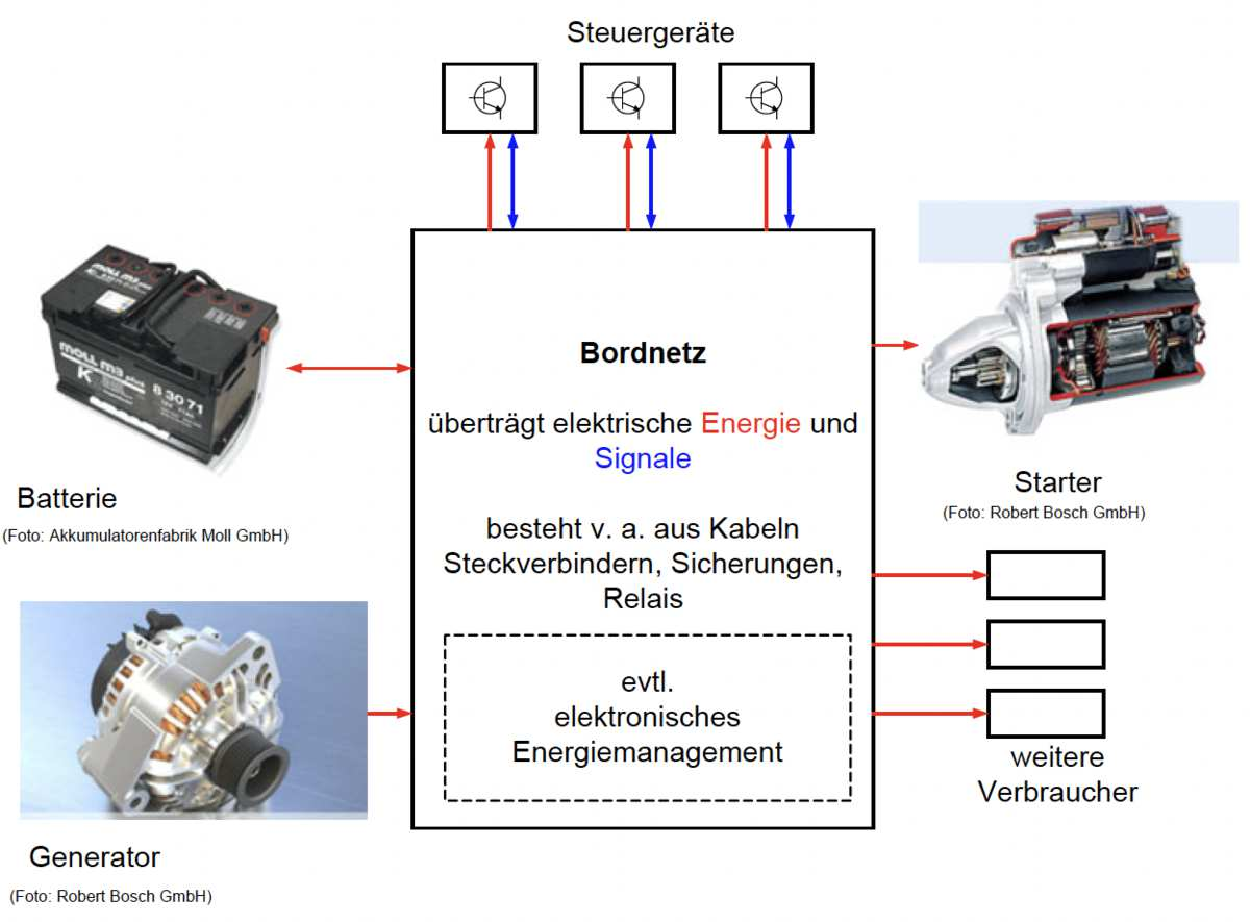
\includegraphics[width=0.7\textwidth]{images/CAN/CAN-1.pdf}
\caption{Überblick über das Bordnetz. (Bild: Kai Borgeest)}
%\label{fig:}%% anpassen
\end{figure}

\textbf{Leitungen}

Um eine unzulässige Erhitzung von Kabeln im normalen Betrieb zu
verhindern, darf die zulässige Stromdichte S nicht überschritten werden.

$S = \frac{I}{A}$ (Stromdichte S, Strom I und dem Leitungsquerschnitt
A)

\textbf{grobe Richtwerte für zulässige Stromdichten}

\begin{itemize}
\item
  Dauerbetrieb $5~A/mm^2$
\item
  kurzzeitige Stromspitzen $10~A/mm^2$
\end{itemize}

Wird die zulässige Stromdichte überschritten, führt die Verlustleistung
$P_V$ in der Leitung zu einer Überhitzung und damit zum Schmelzen, zur
Zersetzung oder zum Brennen des Isoliermaterials oder angrenzender
Strukturen, bei erheblicher Überlast auch zum Schmelzen des Leiters.

\textbf{Verlustleistung beim Strom I}

$P_v = I^2 \cdot R \quad R = \frac{\rho \cdot l}{A}$ (Kupferleitung
$0,0185~\Omega mm^2/m$)

$I = \frac{P}{U}$

\newpage

\textbf{elektrischer Verbraucher 12-V-Bordnetz}

\begin{table}[!ht]% hier: !ht 
\centering 
	\caption{}% \label{tab:}%% anpassen 
\begin{tabular}{@{}lll@{}}
\hline
\textbf{Verbraucher} & \textbf{Leistungsaufnahme P} & \textbf{Strom
I} \\
\hline
Elektro-Kraftstoffpumpe & 250 W & 21 \\
Heckscheibenheizung & 200 W & 17 \\
Innengebläse & 120 W & 10 \\
Kühlerventilator & 120 W & 10 \\
Abblendlicht & 110 W & 9,2 \\
Scheibenwischer & 50 W & 4,2 \\
Bremslicht & 42 W & 3,5 \\
Kennzeichenleuchte & 30 W & 2,5 \\
Standlicht & 8 W & 0,7 \\
\hline
\end{tabular} 
\end{table}

\textbf{Elektro- und Hybridfahrzeugen}

Ab 60 V hat sich der Begriff Hochvoltkabel durchgesetzt. Hochvoltkabel
haben eine geerdete Abschirmung, sind mechanisch besonders stabil und
durch ihre orange Farbgebung auffällig gekennzeichnet.

Hochvoltkomponenten werden durch eine ringförmige Niederspannungsleitung
verbunden (HVIL, High Voltage Interlock Loop), die auf Unterbrechungen
überwacht wird. Wird eine Unterbrechung durch Trennung einer Leitung
oder Öffnung eines Gehäuses erkannt, führt dies zur Abschaltung des
Hochvoltsystems.

\textbf{Klemmenbezeichnungen} (Auswahl)

\begin{table}[!ht]% hier: !ht 
\centering 
	\caption{}% \label{tab:}%% anpassen 
\begin{tabular}{@{}ll@{}}
\hline
\textbf{Nr.} & \textbf{Bezeichnung} \\
\hline
1 & Zündspule (gemeinsame Klemme) \\
4 & Zündspule (Hochspannungsausgang) \\
15 & Positive Batteriespannung, über Schlüsselschalter \\
30 & Positive Batteriespannung \\
31 & Negative Batteriespannung \\
50 & Anlasser (geschaltete Klemme) \\
54 -- 58 & Beleuchtung \\
81 -- 88 & Schalter und Relais \\
B+ & Positive Generatorklemme zur Batterie \\
B & Negative Generatorklemme zur Batterie \\
D+ & Positive Klemme an Generator und Regler für Regelung und Leuchte \\
D & Negative Klemme an Generator und Regler für Regelung und Leuchte \\
DF & >>Dynamo Feld<<, Klemme an Generator und Regler für
Erregerwicklung \\
U, V, W & Drehstromklemmen des Generators \\
\hline
\end{tabular} 
\end{table}

\newpage

\subsection{Mehrspannungsbordnetzes}\label{mehrspannungsbordnetzes}

In Zukunft ist mit neuen Fahrzeugsystemen wie >>Brake-by-Wire<< oder
>>Steer-by- Wire<< zu rechnen, die einen hohen Bedarf an elektrischer
Energie haben. Damit steigen auch die Ströme im Bordnetz an und so
quadratisch die Leitungsverluste. Durch Einsatz einer höheren
Bordnetzspannung kann die gleiche Leistung mit reduzierten Strömen
übertragen werden. Je höher die Spannungen sind, umso geringer werden
die Leitungsverluste.

\begin{figure}[!ht]% hier: !ht
\centering
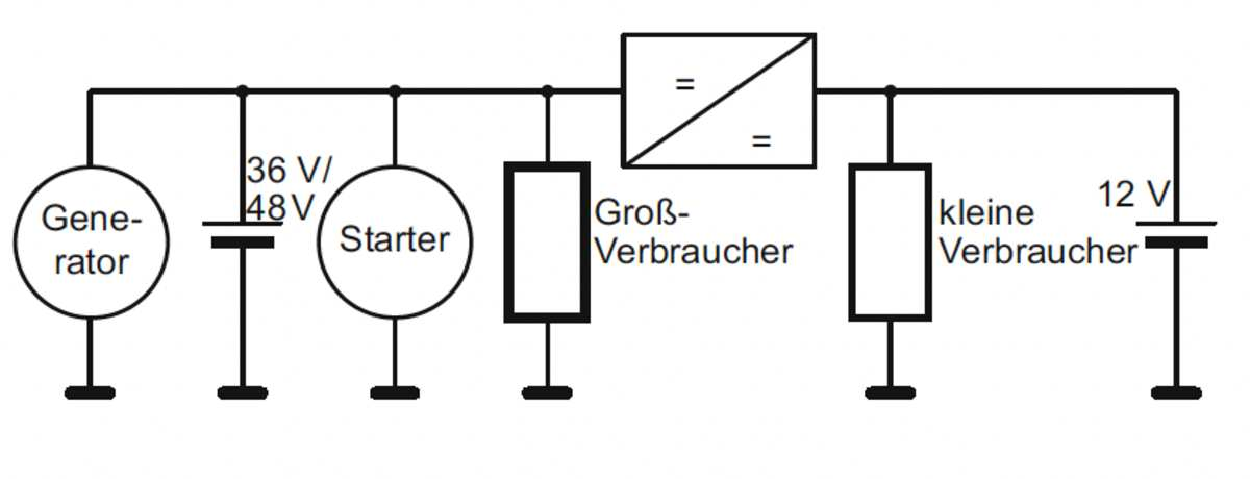
\includegraphics[width=0.7\textwidth]{images/CAN/CAN-2.pdf}
\caption{Struktur eines künftigen Mehrspannungsbordnetzes (Bild: Kai
Borgeest)}
%\label{fig:}%% anpassen
\end{figure}

Kombination aus einem 12-V-Netz für Kleinverbraucher und einem 48-V-Netz
für Großverbraucher. Beide Netze werden über einen Schaltwandler (DC/DC)
gekoppelt.

\newpage

\subsection{Energiemanagement (BMS)}\label{energiemanagement-bms}

\begin{enumerate}
\item
  Batterieüberwachung

  \begin{itemize}
  \item
    Eingriff in die Laderegelung
  \item
    Eingriff in das Motormanagement, um zum Aufladen der Batterie eine
    Mindestdrehzahl zu erzwingen.
  \item
    Ziele

    \begin{enumerate}
    \def\labelenumii{\arabic{enumii}.}
    \item
      Bestimmung des Ladezustandes (State of Charge, SOC)
    \item
      Restlebensdauer der Batterie (State of Health, SOH)
    \item
      Funktionsfähigkeit der Fahrzeugfunktionen, vor allem des Startens
      (State of Function, SOF).
    \end{enumerate}
  \end{itemize}
\item
  automatisch Verbraucher je nach Wichtigkeit und Leistungsbedarf
  abzuschalten oder auch wieder einzuschalten.
\item
  Steuerung eines hybriden Antriebssystems
\end{enumerate}

\textbf{Energiemanagement-Steuergerät / Bordnetzsteuergerät} benötigt
von der Batterie Informationen über Temperatur, Spannung und Strom.

\textbf{Batterietyp} über Diagnosetester dem Energiemanagement
mitteilen, welcher eingebaut wurde.

\textbf{Fremdstartbolzen} der bei Starthilfe anstelle des
Batterie-Minuspols zu verwenden ist, damit das Steuergerät den
Fremdstart registriert und bei seinen Berechnungen berücksichtigt.

\textbf{schweren Unfall} (Signal vom Airbag-Steuergerät) über ein Relais
das Bordnetz spannungsfrei schaltet.

Bei großen Batterien für Hybrid- und Elektrofahrzeuge werden wesentliche
Teile des Energiemanagements in die Batterie integriert.

\newpage

\section{CAN-Bus}\label{can-bus}

CAN-Bus war das erste digitale Bussystem.

\begin{figure}[!ht]% hier: !ht
\centering
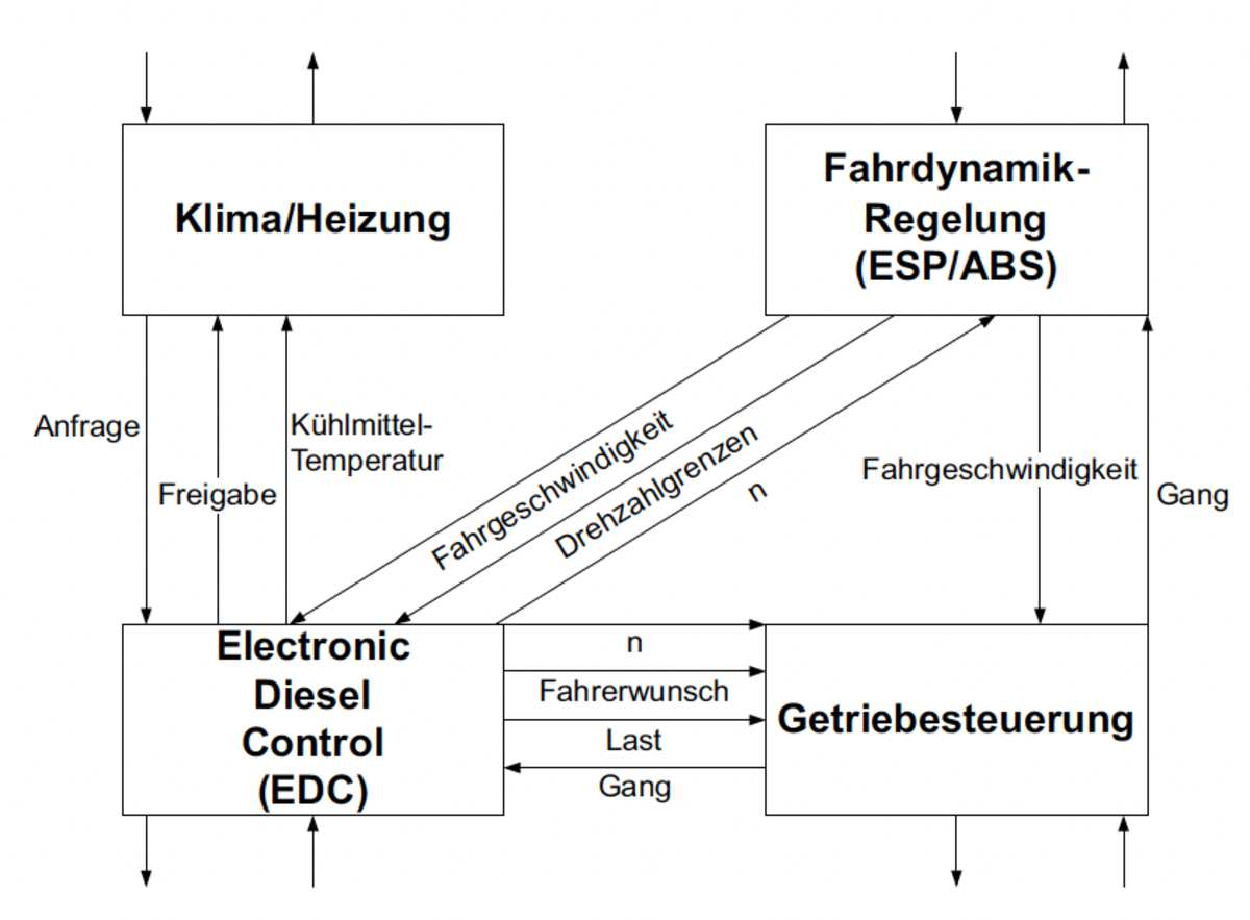
\includegraphics[width=0.7\textwidth]{images/CAN/CAN-3.pdf}
\caption{Ein kleiner Ausschnitt aus der Kommunikationsmatrix zwischen
vier Steuergeräten (Bild: Kai Borgeest)}
%\label{fig:}%% anpassen
\end{figure}

\begin{figure}[!ht]% hier: !ht
\centering
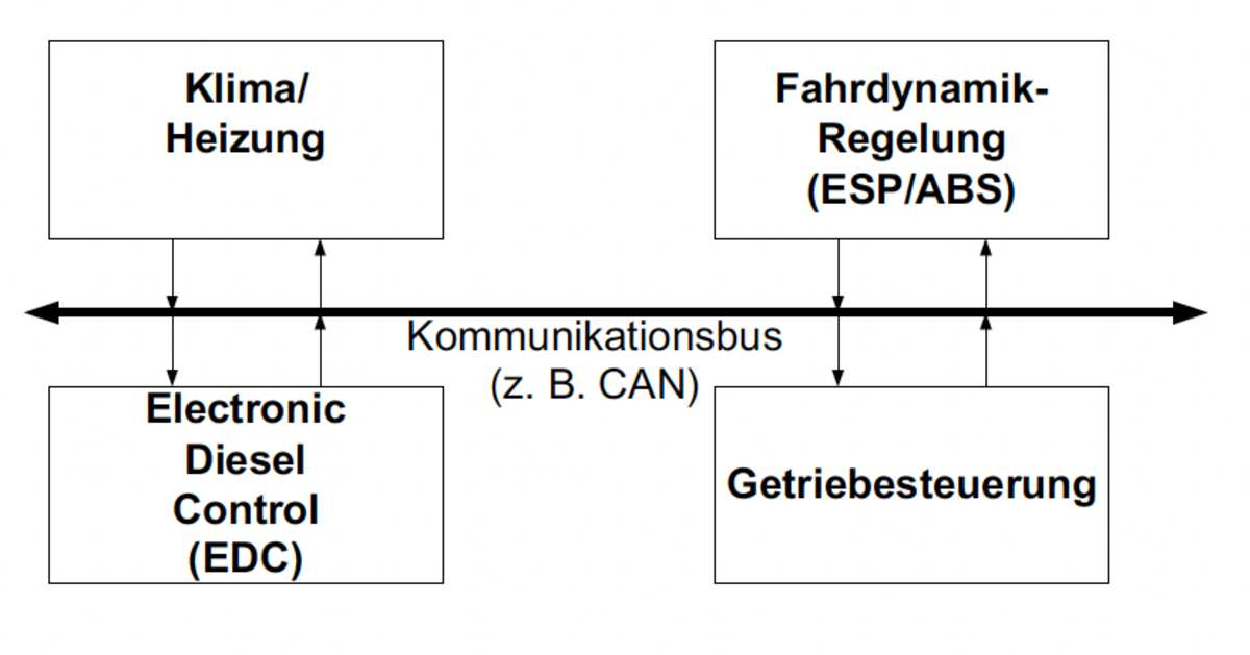
\includegraphics[width=0.7\textwidth]{images/CAN/CAN-4.pdf}
\caption{Vier über einen Bus kommunizierende Steuergeräte (Bild: Kai
Borgeest)}
%\label{fig:}%% anpassen
\end{figure}

\newpage

\textbf{Transceiver} ein Kunstwort aus Transmitter/Receiver, also
Sender/Empfänger

\begin{figure}[!ht]% hier: !ht
\centering
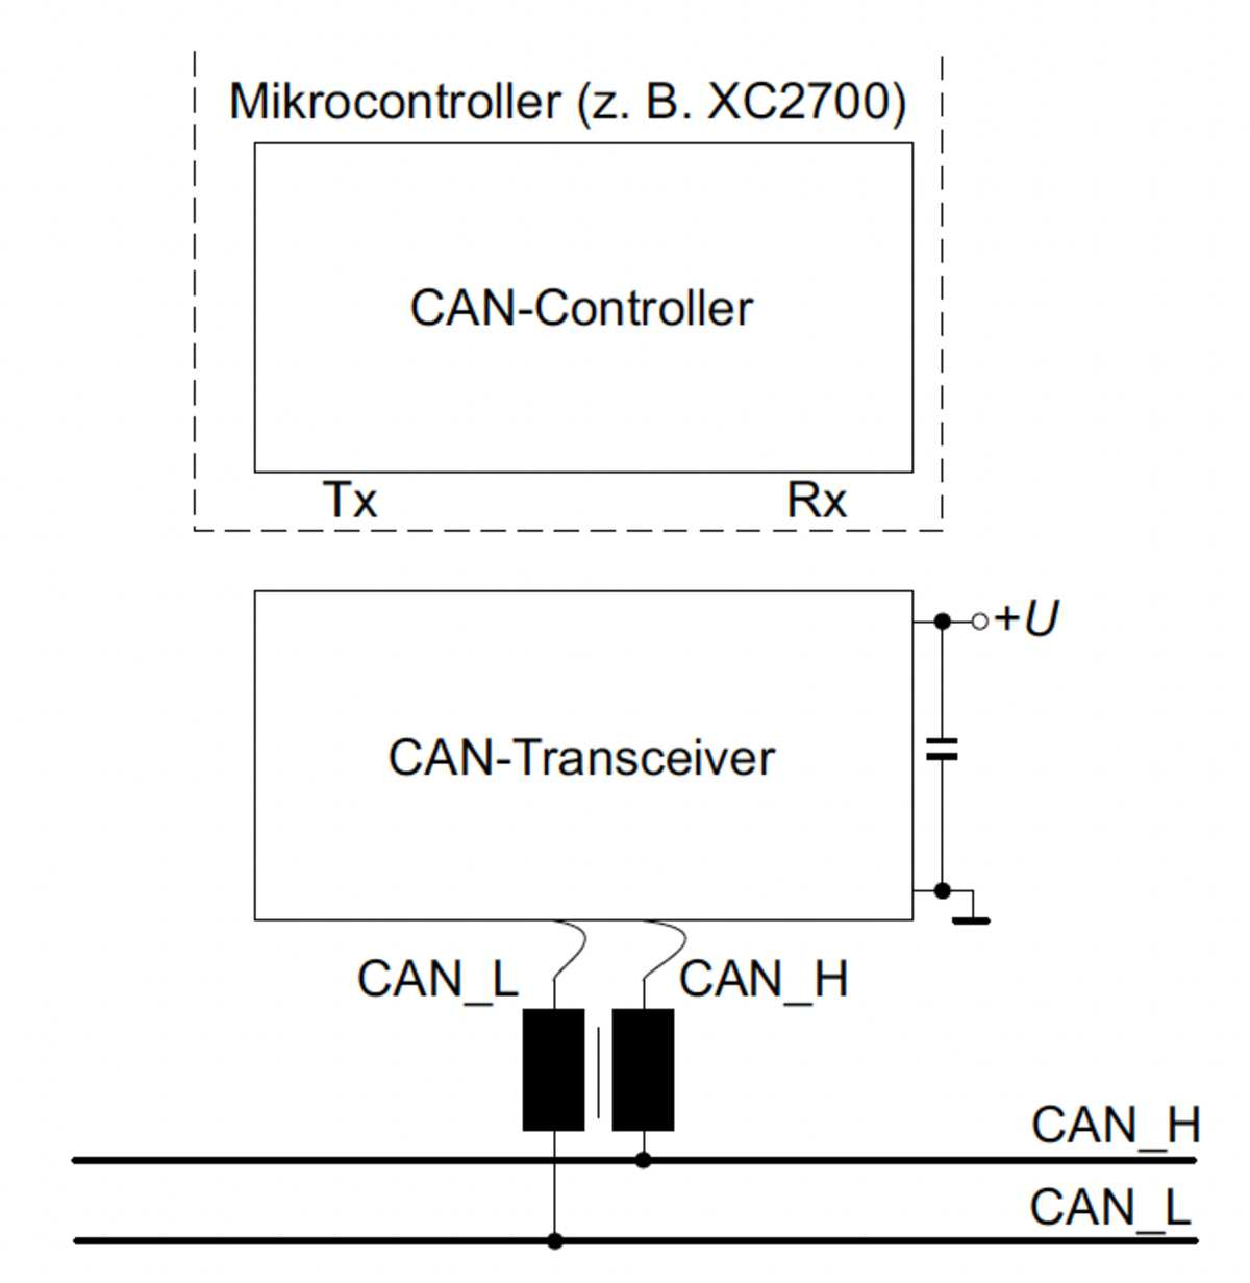
\includegraphics[width=0.5\textwidth]{images/CAN/CAN-5.pdf}
\caption{Umsetzung des OSI-Modells durch die verwendeten Bauelemente.
Der CAN-Controller erzeugt eine Nachricht mit dem gewünschten Inhalt und
sendet sie über die Leitung Tx an den Transceiver. Wenn auf dem Bus eine
Nachricht erscheint, schickt er diese über die Rx-Leitung an den
CAN-Controller, der wiederum Teil eines Mikrocontrollers sein kann, aber
nicht sein muss. Die Bezeichnungen CAN\_H und CAN\_L stehen für >>CAN
high<< und >>CAN low<<. (Bild: Kai Borgeest)}
%\label{fig:}%% anpassen
\end{figure}

\newpage

\subsection{Spannungspegel und
Störsicherheit}\label{spannungspegel-und-stoersicherheit}

Zwei verdrillte Adern stellt einen sinnvollen Kompromiss zwischen
Störfestigkeit und Kosten dar. Das Signal wird über beide Leitungen
entgegengesetzt übertragen.

\textbf{logische 1} soll gesendet werden, wird der Tx-Eingang des
Transceivers vom Controller mit einer Spannung von z. B. 5 V
angesteuert. Der untere PNP-Transistor sperrt, der obere NPN-Transistor
bekommt das invertierte Signal und sperrt ebenfalls. Der Bus behält
seine Ruhespannung von 2,5 V auf beiden Leitungen, die
Spannungsdifferenz zwischen den Busleitungen CAN\_H und CAN\_L ist 0.
Die Sendeschaltung muss nicht wie hier gezeigt mit NPN- und
PNP-Transistoren aufgebaut werden, sondern kann auch mit
Feldeffekt-Transistoren (FET) realisiert werden.

\textbf{logischen 0} leiten beide Transistoren, also wenn der Controller
das Signal am Tx-Eingang auf 0 V legt. In diesem Falle wird die Spannung
auf CAN\_H erhöht, die Spannung auf CAN\_L gesenkt.

\begin{itemize}
\item
  \textbf{CAN\_H} oder >>CAN high<< für Anhebung
\item
  \textbf{CAN\_L} oder >>CAN low<< für Absenkung
\end{itemize}

\newpage

\textbf{High-Speed-CAN}

\begin{itemize}
\item
  3,5 V auf dem CAN\_H und
\item
  1,5 V auf CAN\_L
\item
  Ruhespannung von 2,5V wird über hohe Widerstände (einige 10 -- 100
  $k\Omega$) auf beide CAN-Leitungen gelegt, damit sich die Spannung
  auf den Busleitungen beim Durchschalten der Transistoren verändern
  kann.
\end{itemize}

\begin{figure}[!ht]% hier: !ht
\centering
\includegraphics[width=0.5\textwidth]{images/CAN/CAN-6.pdf}
\caption{Elektrische Ansteuerung und Auswertung des CAN-Busses im
Transceiver (vereinfacht). Links ist der Sender, rechts daneben der
Empfänger eingezeichnet. Ganz rechts ist klein die Erzeugung des
Ruhepotentials von 2,5V (in vielen Highspeed-CAN-Transceivern
integriert) angedeutet (Bild: Kai Borgeest)}
%\label{fig:}%% anpassen
\end{figure}

Der Empfänger vergleicht die Spannungen auf CAN\_H und CAN\_L. Bei einer
logischen 1 liegen beide CAN-Leitungen auf 2,5 V, die Differenz ist 0.
Der nachfolgende Inverter erzeugt aus dieser 0 wieder eine 1. Bei einer
logischen 0 ist zwischen den Spannungen eine Differenz von 2 V
vorhanden. Wenn die Differenzspannung einen sicheren Minimalwert (z. B.
1 V), überschreitet, wird dies zunächst durch eine 1 signalisiert, aus
welcher der Inverter wieder die ursprüngliche 0 erzeugt.

\textbf{Low-Speed-CAN}

\begin{itemize}
\item
  Ruhespannung und rezessive Spannung

  \begin{itemize}
  \item
    5 V am CAN\_L
  \item
    0 V am CAN\_H
  \end{itemize}
\item
  dominante Spannung am

  \begin{itemize}
  \item
    1,4 V oder kleiner CAN\_L
  \item
    3,6 V oder größer am CAN\_H
  \end{itemize}
\end{itemize}

\textbf{Ist eine der beiden Leitungen defekt}, kann sie abgeschaltet
werden (Fault Tolerant CAN). Der symmetrische Betrieb wird dann
verlassen, indem die verbleibende Leitung gegen Masse betrieben wird.

\textbf{Wake-Up} (Aufwecken) Low-Speed-CAN-Transceiver können in einen
Bereitschaftszustand gehen, in dem der Sendeteil abgeschaltet ist, der
Empfangsteil aber bereit bleibt, um ein durch Kommunikation auf dem Bus
oder Aktivierung eines Pins zu ermöglichen.

\textbf{Energieeinsparung} wird ein Teilnetzbetrieb (Partial
Networking), bei dem Steuergeräte, die gerade keine Funktion erfüllen,
ihren Energieverbrauch reduzieren, immer wichtiger. Dieser benötigt ein
selektives Aufwecken einzelner Busteilnehmer.

\newpage

\subsection{Wellenwiderstand und
Abschluss}\label{wellenwiderstand-und-abschluss}

\textbf{Wellenwiderstand} sagt aus, welchen fiktiven Widerstand ein
Signal am Eingang einer Leitung >>sieht<< und damit, welchen Strom die
Quelle in die Leitung einspeist. Ist eine Kenngröße jeder Leitung, also
jedes Leiterpaares.

Wird eine Leitung nicht mit ihrem Wellenwiderstand abgeschlossen, kommt
es zu Reflexionen des Signals an ihren Enden.

\begin{enumerate}
\item
  \textbf{Leitung an den Enden offen zu lassen}

  \begin{itemize}
  \item
    kann vorkommen, wenn am Ende der Leitung sich ein Steuergerät
    befindet, dessen Transceiver einen hohen Eingangswiderstand hat (was
    durchaus üblich ist). In diesem Falle käme es zu einer Reflexion,
    das Signal würde die Leitung wieder zurücklaufen und sich mit
    anderen hinlaufenden Signalen überlagern. Damit würden andere
    Steuergeräte am Bus im schlimmsten Fall einen undefinierten
    Datenzustand empfangen, die Kommunikation auf dem Bus kann
    zusammenbrechen.
  \end{itemize}
\item
  \textbf{Leitung an den Enden kurz zuschließen}

  \begin{itemize}
  \item
    kommt nur bei Fehlern vor
  \end{itemize}
\end{enumerate}

\textbf{High-Speed-CAN} an beiden Enden mit je einem Widerstand von
nominal 120 $\Omega$ abgeschlossen, dies entspricht näherungsweise dem
Wellenwiderstand der verdrillten 2-Draht-Leitung. Um Störströme gezielt
abzuleiten, werden oft zwei Widerstände zu 60 $\Omega$ in Reihe
geschaltet und der Knoten zwischen den beiden Widerständen über einen
Kondensator von wenigen nF auf Masse gelegt.

Zweckmäßigerweise wird man diese beiden Widerstände nicht direkt in den
Kabelbaum einbauen, sondern in die an beiden Busenden sitzenden
Steuergeräte.

\textbf{Low-Speed-CAN} üblich, in jedem Knoten Widerstände jeweils gegen
Masse und Versorgungsspannung vorzusehen. Hersteller empfehlen
Gesamtabschlusswiderstände des Netzwerkes (Parallelschaltung aller
einzelnen Abschlüsse) zwischen 100 $\Omega$ und darüber. Der optimale
Abschlusswiderstand steigt also mit der Anzahl der elektrisch parallel
geschalteten Knoten im Netzwerk.

\newpage

\subsection{Verbindung von
Steuergeräten}\label{verbindung-von-steuergeraeten}

\begin{figure}[!ht]% hier: !ht
\centering
\includegraphics[width=0.5\textwidth]{images/CAN/CAN-7.pdf}
\caption{CAN-Bus mit sternförmiger Anbindung (passiver Stern) (Bild: Kai
Borgeest)}
%\label{fig:}%% anpassen
\end{figure}

\begin{enumerate}
\item
  \textbf{passive Stern}

  \begin{itemize}
  \item
    wird häufig in der Nähe des Armaturenbretts realisiert, evtl.
    existieren auch mehre Sternpunkte.
  \item
    Vorbildlich hat z. B. Audi beim A6 und beim A8 die Sternpunkte
    realisiert. Sämtliche Zugänge treffen sich an den beiden Seiten des
    Armaturenbrettes, die Verbindungen erfolgen über Brückenstecker.
  \end{itemize}
\item
  \textbf{aktiver Stern} bei dem sich ein weiteres Gerät im Sternpunkt
  befände, um jede Verzweigung mit einem eigenen Transceiver
  anzusteuern.

  \begin{itemize}
  \item
    Gateway (aktiver Stern) eines Oberklasse-Fahrzeugs mit vier
    High-Speed-Transceivern (HS) und einem Low-Speed-Transceiver (LS)
    für den langsameren Komfort-CAN. Eine CPU (Mikrocontroller) kann
    gezielt Nachrichten aufarbeiten und an andere Busse weiterleiten.
  \end{itemize}

  \begin{enumerate}
  \def\labelenumii{\arabic{enumii}.}
  \item
    High-Speed-Transceivern (HS)

    \begin{itemize}
    \item
      Antriebs-CAN
    \item
      Kombi-CAN
    \item
      ACC-CAN
    \item
      Diagnose-CAN
    \end{itemize}
  \item
    Low-Speed-Transceiver (LS)

    \begin{itemize}
    \item
      Komfort-CAN
    \end{itemize}
  \end{enumerate}
\end{enumerate}

\begin{figure}[!ht]% hier: !ht
\centering
\includegraphics[width=0.5\textwidth]{images/CAN/CAN-8.pdf}
\caption{Gateway (aktiver Stern) eines Oberklasse-Fahrzeugs mit vier
High-Speed-Transceivern (HS) und einem Low-Speed-Transceiver (LS) für
den langsameren Komfort-CAN. Eine CPU (Mikrocontroller) kann gezielt
Nachrichten aufarbeiten und an andere Busse weiterleiten. (Bild: Kai
Borgeest)}
%\label{fig:}%% anpassen
\end{figure}

Inzwischen ist es üblich, in einem Fahrzeug mehrere elektrisch getrennte
CAN-Busse zu haben, die sich auch in ihren Datenraten unterscheiden
können, aber nicht müssen. Verbunden sind diese dann über einen aktiven
Sternpunkt, der auch als Gateway bezeichnet wird. Während bei Systemen
von geringer Komplexität (bis ca. 5 Steuergeräte im Fahrzeug) evtl. auf
ein Gateway verzichtet wird, besitzen Systeme von mittlerer bis hoher
Komplexität (ab ca. 50 Steuergeräte im Fahrzeug) auf jeden Fall eines.
Das Gateway kann eine zusätzliche Funktion eines möglichst zentralen
Steuergerätes, z. B. des Kombiinstruments sein, mit zunehmender
Komplexität verwendet man als Gateway ein eigenständiges Gerät, welches
nur diese Aufgabe verrichtet.

\chapter{EDC-Elektronische-Dieselsteuerung}
%%ju 31-Dez-22 EDC-Elektronische-Dieselsteuerung.tex
\section{Aufgaben der
Motorsteuerung}\label{aufgaben-der-motorsteuerung}

\begin{enumerate}
\item
  Einspritzung des Kraftstoffes in die Zylinder
\item
  Regelung und Begrenzung von Drehzahl und Geschwindigkeit,
\item
  Regelung des Luftsystems (Abgasrückführung und Ladedruckregelung),
\item
  Abgasnachbehandlung,
\item
  Glühkerzensteuerung und Thermomanagement,
\item
  Zylinderabschaltung,
\item
  Diagnose,
\item
  Wegfahrsperre.
\end{enumerate}

\newpage

\section{Einspritzung}\label{einspritzung}

Quelle: S. 57 \textcite{borgeest:2021:elektronik}.

\begin{figure}[!ht]% hier: !ht
\centering
\includegraphics[width=0.7\textwidth]{images/EDC/EDC-1.pdf}
\caption{Einspritzfunktion eines Dieselsteuergerätes ($\varphi$:
Kurbelwellenwinkel). (Bild: Kai Borgeest)}
%\label{fig:}%% anpassen
\end{figure}

\begin{itemize}
\item
  SG optimalen Zeitpunkt für den Beginn der Einspritzung berechnet und
  die >>richtige<< Menge für die Einspritzung kennt.

  \begin{itemize}
  \item
    Einspritzmenge
  \item
    Zeitpunkt / Spritzbeginn
  \end{itemize}
\item
  Ansteuern der Einspritzventile für jeden Zylinder
\item
  Fahrpedal (Fahrerwunsch)
\item
  Winkeluhr im SG

  \begin{itemize}
  \item
    aktuelle Stellung der Kurbelwelle und Drehzahl
  \item
    zeitlich veränderliche Vorgänge im Motor nicht direkt als Funktion
    der Zeit, sondern als Funktion des Kurbelwellenwinkels
    (winkelsynchron) anzugeben und zu berechnen
  \item
    In der Zeit $\Delta t$ bewegt sich bei der Drehzahl $n$ die
    Kurbelwelle um den Winkel
  \item
    $\Delta \varphi = 6 \cdot n \cdot \Delta t$
    $\quad [^\circ \text{KW} = \text{min}^{-1} \cdot \text{s}]$
  \end{itemize}
\item
  Einspritzung bei

  \begin{itemize}
  \item
    $0^\circ$ bedeutet das der Kolben bei einem als Bezug gewählten
    Zylinder gerade am oberen Totpunkt steht.
  \item
    $-10^\circ$ bedeuten, dass sich die Kurbelwelle noch um
    $10^\circ$ drehen muss, bis der Kolben im Bezugszylinder den OT
    erreicht hat.
  \item
    $+10^\circ$ bedeuten, dass der Kolben schon wieder auf dem Weg vom
    OT nach unten ist.
  \end{itemize}
\end{itemize}

\newpage

\begin{figure}[!ht]% hier: !ht
\centering
\includegraphics[width=0.5\textwidth]{images/EDC/EDC-3.pdf}
\caption{Signale vom Kurbelwellen- und Nockenwellensensor. (Bild: Kai
Borgeest)}
%\label{fig:}%% anpassen
\end{figure}

\textbf{Kurbelwellensensor}

\begin{itemize}
\item
  Impulsgeber, dessen Impulsfrequenz steigt mit der Drehzahl. Durch
  abzählen der Impulse lässt sich der Winkel bestimmen.
\end{itemize}

\textbf{Nockenwellensensor}

\begin{itemize}
\item
  OT-Verbrennung (Bezugsmarke/Referenzmarke) in $^\circ \text{KW}$
\end{itemize}

\begin{figure}[!ht]% hier: !ht
\centering
\includegraphics[width=0.3\textwidth]{images/EDC/EDC-4.pdf}
\caption{Elektromagnetischer Sensor für die Drehzahl der Kurbelwelle.
Die nur im Luftspalt eingezeichneten Magnetfeldlinien schließen sich
über das Zahnrad, dessen Lagerung und über das Gehäuse, welches das
Zahnrad umfasst und den Sensor aufnimmt. Durch Änderung des Feldes wird
in der Spule die Spannung $U_{\text{ind}}$ induziert. (Bild: Kai
Borgeest)}
%\label{fig:}%% anpassen
\end{figure}

\newpage

\textbf{4-Zylinder Motor:}

\begin{itemize}
\item
  $0^\circ (\text{Kolben im OT, Einspritzung Verbrennung}), 180^\circ (\text{UT})$
\item
  und
  $360^\circ (\text{Kolben im OT, Ausstoßen}), 540^\circ (\text{UT})$
\item
  zweideutigkeit (Kolben 2x im OT pro Arbeitsspiel)
\item
  alle 4x-Takte: Ansaugen, Verdichten, Arbeiten/Verbrennen, Ausstoßen
\item
  zwei Kurbelwellenumdrehungen ($720^\circ$), eine
  Nockenwellenumdrehung
\end{itemize}

\begin{figure}[!ht]% hier: !ht
\centering
\includegraphics[width=0.7\textwidth]{images/EDC/EDC-2.pdf}
\caption{Darstellung der vier Takte eines Viertaktmotors von links nach
rechts: a Beginn des Ansaugtaktes ($360-540^\circ$): Bei geöffneten
Einlassventil saugt der sich abwärts bewegende Kolben Luft an. b Ende
des Verdichtungstaktes ($540-720^\circ$): Beide Ventile sind
geschlossen, durch die Aufwärtsbewegung des Kolbens wird die Luft
komprimiert und dadurch erhitzt. c Beginn des Arbeitstaktes
($0-180^\circ$): Der Kraftstoff wird eingespritzt und verbrennt durch
die hohe Lufttemperatur. Dadurch wird der Kolben nach unten gedrückt. d
Ende des Ausstoßtaktes ($180-360^\circ$): Durch das nun geöffnete
Auslassventil drückt der wieder steigende Kolben die Verbrennungsgase
aus dem Zylinder heraus. (Bild: Kai Borgeest)}
%\label{fig:}%% anpassen
\end{figure}

\newpage

\subsection{Berechnung der
Einspritzmenge}\label{berechnung-der-einspritzmenge}

\textbf{Fahrzustände}

\begin{itemize}
\item
  Start, Leerlauf, Fahren
\item
  \textbf{Schubbetrieb} bei Bergabfahrt mit einem niedrigen Gang; in
  diesem Falle bremst der Motor das bergab rollende Fahrzeug.
\item
  \textbf{Teillast und Volllast}
\item
  \textbf{Notlauf} Steuergerät erkennt einen kritischen Zustand oder
\item
  \textbf{Grenzzustände} (z. B. das Abregeln bei Erreichen von Drehzahl-
  oder Geschwindigkeitsgrenzen).
\end{itemize}

Die \textbf{Einspritzmenge} berechnet sich über einen weiten Bereich
näherungsweise proportional aus dem angeforderten Drehmoment
(Fahrerwunsch), bzw. im Leerlauf von der Anforderung des
Leerlaufreglers.

Fahrerwunsch wird vom Gaspedal über einen Pedalwertgeber (PWG, Sensor
der einen Winkel in eine Spannung umsetzt) elektrisch an das Steuergerät
übertragen.

\textbf{weitere Parameter für das Drehmoment bzw. die Einspritzmenge}

\begin{itemize}
\item
  aktuelle Drehzahl
\item
  aktuelle Fahrgeschwindigkeit
\item
  Motorlast
\item
  Temperatur des Motors (gemessen über die Kühlwassertemperatur,
  Öltemperatur),
\item
  Batteriespannung
\item
  Informationen über das Getriebe
\item
  Betriebszustand (z. B. Kaltstart)
\item
  Begrenzungen (z. B. Rauchbegrenzung)
\end{itemize}

\textbf{Mengenberechnung}

\begin{enumerate}
\item
  \textbf{Mengenpfad} oder

  \begin{itemize}
  \item
    berechnet grob die erforderliche Einspritzmenge, passt diese dann
    durch etliche Korrekturrechnungen, Kennfelder, Begrenzungen und
    eventuelle externe Mengeneingriffe auf die exakt benötigte Menge an.
  \end{itemize}
\item
  \textbf{Momentenpfad}

  \begin{itemize}
  \item
    wird zuerst das vom Motor benötigte Drehmoment grob berechnet,
    sämtliche Berechnungen im Steuergerät werden mit Momenten statt mit
    Mengen durchgeführt und erst zum Schluss des Berechnungspfades wird
    die genaue Momentenanforderung in die exakte Einspritzmenge
    umgerechnet.
  \end{itemize}
\end{enumerate}

Bei externen Eingriffen (Signale von anderen Steuergeräten) kann die
Momentenstruktur als >>gemeinsame Sprache<< mehrerer Steuergeräte
vorteilhaft sein, da Getriebesteuergeräte und Fahrdynamiksteuergeräte
intern mit mechanischen Größen und nicht mit Kraftstoffmengen rechnen.

\begin{enumerate}
\item
  \textbf{Voreinspritzung} zur Geräuschminderung

  \begin{itemize}
  \item
    PKW in der Größenordnung von $1 - 2~mm^3$
  \end{itemize}
\item
  \textbf{Haupteinspritzung} Drehmoment

  \begin{itemize}
  \item
    PKW in der Größenordnung von einiger $10~mm^3$
  \end{itemize}
\item
  \textbf{Nacheinspritzung} zur Nachverbrennung von Partikeln im
  Zylinder oder zur Unterstützung der Abgasnachbehandlung.

  \begin{itemize}
  \item
    PKW in der Größenordnung von $1 - 2~mm^3$
  \end{itemize}
\end{enumerate}

Vgl. Wassertropfen ein Volumen von ca. $30~mm^3$

\newpage

\subsection{Berechnung des
Spritzbeginns}\label{berechnung-des-spritzbeginns}

\begin{enumerate}
\item
  \textbf{frühe Einspritzung} führt zu einer zu frühen Verbrennung.
  Dadurch wird bereits eine Kraft von oben auf den Kolben ausgeübt,
  bevor er den OT erreicht. Dies führt zu einem Verlust an Leistung, im
  Extremfall sogar zum Stillstand oder zur Beschädigung des Motors.
  Weiterhin erreicht die Verbrennungstemperatur zu hohe Spitzenwerte,
  die zu einer vermehrten Bildung von Stickoxiden im Abgas führen.
\item
  \textbf{späte Einspritzung} führt dazu, dass der eingespritzte
  Kraftstoff nicht mehr vollständig verbrennt. Dadurch geht ebenfalls
  Leistung verloren und es bildet sich schwarzer Rauch, der Partikel
  enthält. Bei noch späterer Einspritzung wird der Kraftstoff völlig
  unverbrannt ausgestoßen, das Abgas färbt sich bläulich und riecht nach
  Diesel. Im Extremfall, wenn unverbrannter Kraftstoff sich als
  Flüssigkeit in der Kolbenmulde ansammelt, kommt es zum Motorschaden.
\end{enumerate}

Bereits bei einer Abweichung des Spritzbeginns um $1^\circ \text{KW}$
lassen sich die gültigen Abgasgrenzwerte nicht mehr einhalten.

Der \textbf{optimale Spritzbeginn} ist keine Konstante, sondern er hängt
vom Motor und von mehreren Betriebsparametern ab. (leistungsoptimierte,
abgasoptimierte Spritzbeginn)

\textbf{Parameter}

\begin{itemize}
\item
  Drehzahl und die Einspritzmenge

  \begin{itemize}
  \item
    Sowohl mit steigender Drehzahl als auch mit zunehmender Menge wird
    der Spritzbeginn nach früh verschoben.
  \end{itemize}
\item
  Temperatur des Motors
\item
  Temperatur der Ansaugluft
\item
  atmosphärische Druck.
\end{itemize}

Im Steuergerät wird der Zusammenhang zwischen den gemessenen Parametern
und dem daraus ermittelten Spritzbeginn durch Formeln oder über
Kennlinien und Kennfelder, also über Wertetabellen dargestellt. Diese
werden zunächst mit Erfahrungswerten gefüllt, dann erfolgt am Prüfstand
eine experimentelle Optimierung.

\newpage

\subsection{Ansteuerung des
Einspritzsystems}\label{ansteuerung-des-einspritzsystems}

\begin{figure}[!ht]% hier: !ht
\centering
\includegraphics[width=0.5\textwidth]{images/EDC/EDC-5.pdf}
\caption{Überblick über ein Common-Rail-Einspritzsystem. (Bild: Kai
Borgeest)}
%\label{fig:}%% anpassen
\end{figure}

\textbf{Common-Rail-System}

\textbf{Vorteil von Common Rail} ist, dass permanent Kraftstoff
einspritzbereit unter einem hohen, über mehrere Einspritzungen konstant
regelbaren Druck verfügbar ist.

\textbf{Nachteil von älteren Einspritzsystemen} (Reihenpumpen,
Einzelpumpen, Verteilerpumpen, Pumpe-Düse, Pumpe-Leitung-Düse) Druck ist
nur zu bestimmten Zeiten, in denen ein Nocken einen Pumpenkolben
betätigt verfügbar.

\begin{itemize}
\item
  \textbf{Rail} rohrförmiger Druckbehälter mit Kraftstoff
\item
  Über kurze Leitungen ist je ein Injektor (Einspritzventil) pro
  Zylinder mit dem Rail verbunden.
\item
  Der Injektor kann vom Steuergerät (ECU) zu definierten Zeiten zur
  Einspritzung geöffnet werden.

  \begin{itemize}
  \item
    \textbf{Piezo-Injektoren} und \textbf{elektromagnetischen
    Injektoren}
  \end{itemize}
\item
  Die eingespritzte Menge hängt von der elektrischen Ansteuerdauer (die
  ungefähr der Dauer entspricht, in der der Injektor geöffnet ist) und
  vom Druck im Rail ab.
\item
  Den Druck im Rail bis 2700 bar, bei LKW bis 3000 bar, erzeugt eine
  Kolbenpumpe.
\item
  Aufgrund der Systemkosten, des Energieaufwandes und der
  Druckwellenproblematik in den Leitungen bei Drücken oberhalb 2000 bar
  arbeiten einige neue Systeme mit einem Raildruck unterhalb 1000 bar
  und erhöhen erst unmittelbar vor der Einspritzung, idealerweise erst
  im Injektor, den Druck über einen hydraulischen Übersetzerkolben auf
  den Einspritzdruck von z. B. 2500 bar.

  \begin{itemize}
  \item
    APCRS (Amplifier Piston Common Rail System) oder druckverstärktes
    Common Rail. Ein Pilotsystem ist das seit 2011 in LKW-Motoren
    eingesetzte >>X-Pulse<< - System von Daimler.
  \end{itemize}
\end{itemize}

\newpage

\subsection{Ansteuerung der
Injektoren}\label{ansteuerung-der-injektoren}

\begin{figure}[!ht]% hier: !ht
\centering
\includegraphics[width=0.5\textwidth]{images/EDC/EDC-8.pdf}
\caption{Ansteuerschaltung für Common-Rail-Injektoren mit Magnetventilen
(Prinzip). (Bild: Kai Borgeest)}
%\label{fig:}%% anpassen
\end{figure}

\textbf{Injektoren mit Magnetventil}

\begin{figure}[!ht]% hier: !ht
\centering
\includegraphics[width=0.7\textwidth]{images/EDC/EDC-6.pdf}
\caption{Injektors mit Magnetventil (bei Bosch bis zur Generation 2.16),
oben geöffnet, unten geschlossen. 1 Kraftstoff-Rücklauf, 2 elektrischer
Anschluss, 3 Elektromagnet, 4 Kraftstoff-Zulauf, 5 Ventilkugel, 6
Ablaufdrossel, 7 Zulaufdrossel, 8 Steuerraum, 9 Druckkolben, 10
Kraftstoff, 11 Nadel. (Bild: Robert Bosch GmbH)}
%\label{fig:}%% anpassen
\end{figure}

\emph{Wirkungskette:} Injektor öffnen $\to$ Steuergerät $\to$
Bestromung des Elektromagneten $\to$ Anzug des Ankers $\to$ Anheben
der Nadel $\to$ Einspritzung

\newpage

\begin{figure}[!ht]% hier: !ht
\centering
\includegraphics[width=0.5\textwidth]{images/EDC/EDC-7.pdf}
\caption{Zeitlicher Verlauf des Stromes durch einen Common-Rail-Injektor
bei einer Voreinspritzung und einer Haupteinspritzung. 1 Skalenteilung
entspricht vertikal einem Strom von 5 A, horizontal einer Dauer von 400
$\mu s$. (Bild: Kai Borgeest)}
%\label{fig:}%% anpassen
\end{figure}

Das Problem liegt nun darin, möglichst schnell den vollen Strom zu
erreichen, um den Anker hochzureißen. Dies lässt sich wegen der
Leitungsinduktivitäten nicht mit Hilfe der Fahrzeug-Batterie
realisieren. Stattdessen wird ein hinreichend großer Kondensator, auch
Booster-Kondensator genannt, im Steuergerät auf eine Spannung in der
Größenordnung 70 -- 90 V aufgeladen, der die Energie für den Anzug
liefert.

\begin{itemize}
\item
  Das erste Stromniveau von ca. 20 A ist der \textbf{Anzugsstrom}, der
  möglichst schnell den Anker heben soll. Eine sehr kurze Einspritzung
  wie die Voreinspritzung kann bereits während dieser Anzugsphase wieder
  enden. Nach einer Dauer von etwa einer halben Millisekunde kann davon
  ausgegangen werden, dass der Anker angezogen ist.
\item
  Von nun an genügt ein kleinerer Strom von z.B. 13 A, der
  \textbf{Haltestrom}, um den Anker in dieser Position zu halten.
\item
  Der zackige Verlauf der Stromniveaus ist darauf zurückzuführen, dass
  der Strom durch Ein- und Ausschalten von Transistoren um den mittleren
  Wert geregelt wird.
\end{itemize}

\textbf{Piezo-Injektoren}

Deren Aktorelement besteht aus einer piezoelektrischen Keramik die sich
bei Anlegen der Spannung um einige $10~\mu m$ dehnt. Über einen
hydraulischen Übersetzter betätigt das Piezo-Element ein Servoventil,
welches das Öffnen der Nadel ermöglicht.

\textbf{Vorteil} gegenüber einem Magnetventil ist ein kürzerer Verzug
zwischen der elektrischen Ansteuerung und dem Beginn der Einspritzung.

Aus elektrischer Sicht verhält sich ein Piezo-Injektor nicht wie eine
Spule, sondern wie ein Kondensator, der zum Einspritzen aufgeladen und
zum Schließen wieder entladen wird.

\begin{figure}[!ht]% hier: !ht
\centering
\includegraphics[width=0.5\textwidth]{images/EDC/EDC-9.pdf}
\caption{Vergleich zwischen Magnetventil-Injektor (rechts) und
Piezo-Injektor (Mitte). Links wird ein Detail einer Düsennadel gezeigt.
(Foto: Robert Bosch GmbH)}
%\label{fig:}%% anpassen
\end{figure}

\newpage

\subsection{Regelung des Raildrucks}\label{regelung-des-raildrucks}

\textbf{hoher Raildruck} ist wünschenswert, um eine feine Zerstäubung
des Kraftstoffs im Brennraum zu erreichen.

\textbf{Leerlauf} würde man mit einem maximalen Einspritzdruck von fast
3000 bar arbeiten, wäre der Motor unzumutbar laut und es wäre auch
schwierig, bei solchen hohen Drücken mit entsprechend kurzen
Ansteuerdauern kleine Mengen noch präzise darzustellen.

Man wird also zuerst abhängig vom Fahrzustand einen geeigneten Druck
auswählen und dann erst die Ansteuerdauer als Funktion der gewünschten
Menge und des Raildrucks berechnen.

\textbf{Raildrucksensoren} piezoresistive Sensoren, bei denen Änderungen
des Druckes in Änderungen des elektrischen Widerstandes umgesetzt
werden. Sie enthalten eine Metallmembran, die durch den Druck
durchgebogen wird. Auf dieser Membran sind vier Dehnungsmessstreifen so
aufgedampft oder mit Leitpaste aufgedruckt, dass zwei Streifen mit
zunehmender Biegung gestaucht, die anderen beiden gedehnt werden. Die
vier Streifen sind zu einer Wheatstone-Brücke verschaltet, in deren
Diagonalzweig eine zum Druck näherungsweise proportionale Spannung
abgegriffen werden kann. Heutige Sensoren enthalten bereits eine
Auswerteelektronik, welche die Brückenspannung auf die gewünschte
Ausgangsspannung umrechnet und Temperatureinflüsse kompensiert.

\newpage

\section{Drehzahlregelung}\label{drehzahlregelung}

\textbf{Änderung der Drehzahl} ergibt sich aus der

\begin{itemize}
\item
  Einspritzmenge, die wiederum vom Fahrerwunsch abhängt und
\item
  Last, die z. B. vom Fahrzeuggewicht und der Steigung abhängt.
\end{itemize}

\textbf{Sonderfall Leerlauf} wenn der Motor durch das Auskuppeln oder
weil kein Gang eingelegt ist, keinen Kraftschluss mit den Rädern hat und
der Fahrer kein Gas gibt, erwarten wir vom Motor einen ruhigen
gleichmäßigen Lauf ohne hörbare Drehzahlschwankungen.

\textbf{Leerlaufregler} benötigt zunächst eine Solldrehzahl.

\begin{itemize}
\item
  \textbf{zu hohe Leerlaufdrehzahl} würde den Kraftstoffverbrauch, die
  Lautstärke und die Emissionen von Schadstoffen erhöhen.
\item
  \textbf{zu niedrige Deerlaufdrehzahl} würde zu einem trägen
  Anfahrverhalten führen und der Generator könnte nicht mehr die
  benötigte Bordnetzspannung erzeugen.
\item
  Ein typischer Wert liegt bei $750~min^{-1}$.
\end{itemize}

\newpage

\section{Regelung des Luftsystems}\label{regelung-des-luftsystems}

\textbf{motorische Verbrennung} ist auf eine ausreichende Luftzufuhr
angewiesen. Reicht die Luft nicht aus, verbrennt der Kraftstoff
unvollständig. In Folge entstehen Schadstoffe und der Motor kann die
geforderte Leistung nicht bringen.

\textbf{Luftmangel erwünscht} der Verbrennungsprozess des Dieselmotors
ist mit höheren Spitzentemperaturen (zwischen $1000^\circ \text{C}$
und $2000^\circ \text{C}$) als bei Ottomotoren verbunden. Bei solch
hohen Temperaturen reagiert auch der in der Luft enthaltene Stickstoff
mit dem Sauerstoff. Es entstehen Stickoxide, vor allem Stickstoffmonoxid
(NO) und Stickstoffdioxid (NO2).

\textbf{Abgasrückführung (AGR) oder Exhaust Gas Recirculation (EGR)}
indem ein Teil des Abgases wieder zum Einlass des Zylinders rückgeführt
wird.

\textbf{Aufladen} um die Luftversorgung zu verbessern, saugt der Motor
nicht nur selbst Umgebungsluft an, sondern ein Turbolader pumpt
zusätzlich Luft in den Motor.

\newpage

\subsection{Abgasrückführung}\label{abgasrueckfuehrung}

\begin{itemize}
\item
  einen Teil der frischen Verbrennungsluft durch sauerstoffarmes Abgas
  zu ersetzen und damit die NOx-bildende Temperaturspitze bei der
  Verbrennung zu senken.
\item
  das hauptsächlich aus Wasser und Kohlendioxid bestehende Abgas eine
  höhere Wärmekapazität als Frischluft hat und so ebenfalls zur Senkung
  der Spitzentemperatur beiträgt.
\item
  Stickstoff, Sauerstoff, Kohlendioxid

  \begin{itemize}
  \item
    Stickstoff (N2) ist sowohl im Frischgas als auch im Restgas
    enthalten.
  \item
    Sauerstoff-Anteil (O2) ist im Abgas gegenüber dem Frischgas
    zumindest stark reduziert.
  \item
    Erhöht ist im Abgas der Anteil an Kohlendioxid (CO2) und Wasser
    (H2O) im gasförmigen Zustand.
  \end{itemize}
\item
  verschlechtert die Verbrennung künstlich und senkt so nicht nur den
  Stickoxid-Ausstoß, sondern auch die Motorleistung. Gleichzeitig
  entstehen mehr Rußpartikel durch die kältere Verbrennung.
\item
  Hochdruckrückführung und Niederdruckrückführung
\end{itemize}

\textbf{Abgasrückführrate} dient als Regelgröße. - Die maximal bei
PKW-Dieselmotoren eingesetzten Rückführraten liegen in der Größenordnung
um 50 \%, d.~h. die Hälfte der Zylinderfüllung stammt aus dem Abgas, der
Rest ist Frischluft. - Sobald die Rückführrate vom Sollwert abweicht, -
steigt entweder die \textbf{NOx-Emission} wieder drastisch an oder -
verbunden mit einem Leistungsverlust und einer Verkokung des Turboladers
die \textbf{Ruß-Emission}.

\begin{figure}[!ht]% hier: !ht
\centering
\includegraphics[width=0.5\textwidth]{images/EDC/EDC-10.pdf}
\caption{Regelung der Abgasrückführrate. (Bild: Kai Borgeest)}
%\label{fig:}%% anpassen
\end{figure}

\newpage

\subsection{Sensorik}\label{sensorik}

Luftmassenmesser (LMM), auch MAF (Mass Airflow Meter) misst die
angesaugte Frischluftmasse.

\begin{itemize}
\item
  Die \textbf{ältesten Luftmassenmesser} bestanden aus einer Klappe, die
  durch den Luftstrom angehoben wurde. Über ein Potenziometer konnte
  dann der Winkel dieser Klappe gemessen werden.
\item
  \textbf{Hitzdrahtsensoren}
\item
  \textbf{Heißfilm-Sensoren}

  \begin{itemize}
  \item
    in der Mitte des Sensorelements befindet sich eine beheizte Zone
    (4), auf beiden Seiten der Heizung befinden sich Temperatursensoren
    (M1 und M2).
  \item
    \emph{Wenn keine Luft} durch den Sensor strömt, stellt sich eine
    symmetrische Temperaturverteilung um die Heizung ein und beide
    Sensoren messen die gleiche Temperatur.
  \item
    \emph{Wenn nun Luft} (7) über die Oberfläche strömt, dann wird der
    in Strömungsrichtung vordere Sensor durch die Luft abgekühlt. Da die
    Luft über der Heizfläche Wärme aufnimmt, wird der hintere Sensor
    schwächer gekühlt.
  \item
    \emph{Temperaturdifferenz} vor und hinter der Heizfläche wird als
    Maß für die vorbeiströmende Luftmasse und auch für die
    Strömungsrichtung benutzt.
  \item
    Die vorbeiströmende Luft enthält Staub und Öldämpfe aus dem
    Kurbelgehäuse des Motors. Der Sensor muss trotzdem über die gesamte
    Fahrzeuglebensdauer präzise messen. Grobe Abweichungen können die
    Motorsteuergeräte über Plausibilitätsprüfungen selbst erkennen und
    als Defekt melden.
  \end{itemize}
\end{itemize}

\begin{figure}[!ht]% hier: !ht
\centering
\includegraphics[width=0.5\textwidth]{images/EDC/EDC-11.pdf}
\caption{Aufbau und Prinzip des Heißfilm-Luftmassenmessers. (Bild:
Robert Bosch GmbH)}
%\label{fig:}%% anpassen
\end{figure}

\textbf{Lambda-Sonde} misst Restsauerstoff im Abgas

\newpage

\subsection{Aufladung}\label{aufladung}

Die \textbf{Luftmenge}, die ein Motor aufnehmen kann, wenn der Kolben im
Einlasstakt als saugende Pumpe wirkt, ist bei \textbf{Atmosphärendruck}
durch das Volumen des Zylinders begrenzt.

Erhöhen lässt sich die \textbf{Luftmenge}, wenn die Luft mit einem
\textbf{Überdruck} in den Zylinder gepresst wird. Dadurch verbrennt der
Kraftstoff in den Phasen, in denen eine große Menge eingespritzt wird,
besser und so entsteht weniger Rauch. Darüber hinaus lässt mit einer
größeren Luftfüllung auch mehr Kraftstoff verbrennen und mehr Leistung
erzeugen.

Tatsächlich lässt sich mit einer Verdopplung des Ladedrucks der gleiche
Effekt wie mit einer Verdopplung des Hubraums erzielen. Üblich sind
Ladedrücke bis zum 2,5-fachen Atmosphärendruck.

Ein \textbf{Turbolader} besteht aus einem Pumpenrad im Ansaugtrakt, das
über eine Welle von einer Turbine angetrieben wird. Die Turbine wird
durch die Energie im Abgasstrom angetrieben.

\begin{itemize}
\item
  \textbf{Vorteil} das die Abgasenergie sinnvoll genutzt wird und den
\item
  \textbf{Nachteil} das insbesondere bei kleinen Drehzahlen die Energie
  im Abgas nicht ausreicht, um einen nennenswert erhöhten Ladedruck
  aufzubauen. Dieser Drehzahlbereich wird umgangssprachlich auch als
  Turboloch bezeichnet und ist für den Fahrer spürbar.
\item
  \textbf{Aufgabe Motorsteuergerät} Ladedruck zu regeln und eine
  schädliche Drucküberhöhung zu vermeiden.

  \begin{itemize}
  \item
    Da der Ladedruck einen erheblichen Einfluss auf das Fahrverhalten
    und den Kraftstoffverbrauch hat, können Steuergeräte eventuell die
    Führungsgrößen passend zum messbaren Fahrstil auswählen. Selten wird
    die Abgastemperatur vor der Turbine gemessen, um den Turbolader vor
    Überhitzung schützen zu können.
  \end{itemize}
\end{itemize}

\newpage

\section{Abgasnachbehandlung
(Ergänzen)}\label{abgasnachbehandlung-ergaenzen}

\textbf{Maßnahmen zur Absenkung der Stickoxidemissionen}
Abgasrückführung oder späte Einspritzung erhöhen beim Dieselmotor die
Partikelemissionen.

\textbf{Maßnahmen zur Reduktion der Partikelemissionen} zu erhöhten
Emissionen von Stickoxiden.

\textbf{Möglichkeiten um schädliche Abgase zu minimieren}

\begin{enumerate}
\item
  ein Kompromiss zwischen Stickoxiden und Partikeln wird gesucht,
\item
  der Motor wird auf minimale NOx-Emissionen optimiert, die dabei
  zusätzlich entstehenden Partikel werden gefiltert,
\item
  der Motor wird auf minimale Partikelemissionen optimiert, die dabei
  zusätzlich entstehenden Stickoxide werden gefiltert oder
\item
  eine Abgasnachbehandlung reduziert zusätzlich NOx-Emissionen und
  Partikelemissionen.
\end{enumerate}

\begin{figure}[!ht]% hier: !ht
\centering
\includegraphics[width=0.5\textwidth]{images/EDC/EDC-13.pdf}
\caption{Umfangreich ausgestattetes Partikelfiltersystem mit zwei
Oxidationskatalysatoren (OK), Partikelfilter (DPF), Temperatur-,
Differenzdruck- und Rußsensor und zusätzlicher Kraftstoffeinspritzung in
den Abgastrakt. (Bild: Kai Borgeest)}
%\label{fig:}%% anpassen
\end{figure}

\begin{figure}[!ht]% hier: !ht
\centering
\includegraphics[width=0.5\textwidth]{images/EDC/EDC-14.pdf}
\caption{System zur selektiven katalytischen Reduktion (SCR) mit
Harnstoff-Einspritzung, Oxidations-Katalysatoren (OK) und einem
Ammoniak-Sperrfilter (SF). Da beide Steuergeräte über den CAN-Bus
kommunizieren, kann die Zuordnung der Sensoren zu den Steuergeräten auch
anders als im Bild erfolgen. (Bild: Kai Borgeest)}
%\label{fig:}%% anpassen
\end{figure}

\newpage

\section{Abgasskandal}\label{abgasskandal}

2015 wurde die Öffentlichkeit über die Medien informiert, dass
Automobilhersteller bei der Feststellung von Abgaswerten manipulierten,
um Fahrzeuge in den Markt zu bringen, die ohne Manipulationen nicht die
gesetzlichen Grenzwerte einhalten.

In der Vergangenheit wurde auf einem Rollenprüfstand ein genormter
Testzyklus (\textbf{NEFZ}, Neuer Europäischer Fahrzyklus) gefahren, die
Abgase während dieses Zyklus wurden gemessen und mit den gesetzlichen
Grenzwerten verglichen. Dieser Zyklus vermied emissionskritische
Situationen wie realistische Beschleunigungen und hohe
Geschwindigkeiten, außerdem enthielt er hohe Stillstandsanteile.

Der \textbf{Kern des Abgasskandals} lag nicht in der Verwendung eines
unrealistischen Zyklus, sondern darin, dass viele Fahrzeughersteller
Funktionen in der Software des Motorsteuergeräts oder des
Getriebesteuergeräts implementiert haben, die einen derartigen
Testzyklus von einer realen Straßenfahrt unterscheiden können.

Die bloße Erkennung ist \textbf{legal}, so muss z. B. das ABS
deaktiviert werden, wenn auf dem Rollenprüfstand nur die Antriebsräder
drehen, nicht hingegen die anderen Räder.

\textbf{Illegal} ist hingegen, das Verhalten des Motorsteuergerätes so
zu verändern, dass auf dem Prüfstand der Motor mit anderen Parametern
betrieben wird und damit faktisch im Straßenverkehr ein anderer Motor
als bei der Typprüfung eingesetzt wird (>>Cycle Beating<<). Auf dem
Prüfstand werden Abgasrückführung und Abgasnachbehandlung so geregelt,
dass die gesetzlichen Grenzwerte eingehalten werden, im Verkehr werden
diese Einrichtungen abgeschaltet oder vermindert eingesetzt.

Die \textbf{Unterscheidung zwischen Prüfstand und Straße} erfolgt über
die Auswertung von Fahrprofilen, der Umgebungsbedingungen (einige
Fahrzeuge reduzieren abgasreinigende Maßnahmen unterhalb
$17^\circ \text{C}$, weil für den NEFZ eine Mindesttemperatur von
$20^\circ \text{C}$ vorgeschrieben war) oder im einfachsten Fall über
einen Timer, der den Prüfstandsmodus nach Ablauf der Prüfzyklusdauer
abschaltet. Häufige illegale Eingriffe („Abschaltfunktionen>>) ins
Motormanagement sind z. B. unterschiedliche Abgasrückführraten oder
unterschiedliche SCR-Betriebsstrategien am Prüfstand und im
Straßenverkehr.

Für Neuzulassungen wurde 2017 in Europa ein realistischerer Testzyklus
im Rahmen der \textbf{WLTP} (Worldwide Harmonized Light Vehicles Test
Procedure) eingeführt, dieser wurde bereits vor etlichen Jahren
definiert, seine Einführung aber immer wieder verzögert.

Neu eingeführt wurde in der EU eine zusätzliche Straßenfahrt mit
Abgasmessung (Real Driving Emissions, \textbf{RDE}), eine Erkennung der
Abgasmessung wurde so erheblich erschwert.

\newpage

\section{Thermomanagement}\label{thermomanagement}

\textbf{Ziel} nach dem Start schnell die optimale Betriebstemperatur des
Motors von ca. $90^\circ \text{C}$ zu erreichen und dann zu halten.

\textbf{mechanisch angetriebene Wasserpumpe} und über eine
Zweipunktregelung mit Hilfe eines \textbf{Thermostaten}.

\begin{itemize}
\item
  Der Thermostat bewirkt, dass bei noch kaltem Motor das Kühlwasser
  zunächst nicht über den Luftwärmetauscher (Kühler) fließt, sondern nur
  in einem kleinen Kreislauf.
\end{itemize}

\textbf{elektrisch angetriebene Wasserpumpe}

\begin{itemize}
\item
  deren Verbreitung allerdings die hohe Leistung des Elektromotors
  entgegensteht. -
\item
  bei stehendem Motor z. B. um einen überhitzten Motor kontrolliert
  abzukühlen, ohne einen Temperaturschock des Motors zu riskieren.
\item
  Die erwähnte Kühlwassertemperatur von $90^\circ \text{C}$ beinhaltet
  einen großen \textbf{Sicherheitsspielraum}, weil die Flüssigkeit je
  nach Überdruck im Kühlsystem und chemischer Zusammensetzung erst bei
  etwa $110$ bis $120^\circ \text{C}$ zu sieden beginnt. Eine
  geregelte Wasserpumpe ermöglicht eine Verkleinerung des
  Sicherheitsspielraumes zugunsten des Motorwirkungsgrades.
\end{itemize}

\textbf{Thermosiphon-Kühlung} Motoren ohne Wasserpumpe, bei denen die
Konvektion (warmes Kühlmittel steigt aufgrund geringerer Dichte auf)
genügte, das Kühlwasser umzuwälzen. \textbf{Energieeinsparung} bei
schwacher Belastung des Motors die Wasserpumpe stillzulegen und zu
überbrücken, wenn der Kühlkreis so ausgelegt ist, dass durch Konvektion
eine ausreichende Kühlung sichergestellt ist.

\textbf{Gebläse mit einem Lüfterrad} hinter dem Kühler, das den
Luftstrom unterstützt, wenn der Fahrtwind nicht ausreicht.

\begin{itemize}
\item
  Das Gebläse wird vom Motorsteuergerät abhängig von der
  Kühlwassertemperatur gesteuert.
\item
  Eventuell wird es auch nach Abstellen des Fahrzeugs und Ausschalten
  der Zündung noch angesteuert. In diesem Falle muss das Steuergerät
  während des Lüfternachlaufs auch noch seine eigene Spannungsversorgung
  aufrechterhalten.
\item
  Bei größeren Motoren ist die \textbf{Leistung elektrischer Lüfter} zu
  hoch für das Bordnetz, in diesem Fall wird der Lüfter mechanisch über
  eine Ölkupplung (Visco-Kupplung) oder zukünftig evtl. über eine
  Kupplung aus Formgedächtnislegierungen angetrieben.
\end{itemize}

\textbf{elektrisch verstellbare Jalousie} vor dem Kühler, diese öffnet
bei hohem Kühlbedarf, ansonsten schließt sie ganz oder teilweise und
kann so auch die Aerodynamik des Fahrzeugs verbessern.

\textbf{elektrische Zuheizer} um schnell die Betriebstemperatur zu
erreichen, werden bereits heute bei Dieselmotoren mit hohem Wirkungsgrad
(und damit geringer Verlustleistung) im Kühlwasserkreislauf oder auch im
Ansauglufttrakt verwendet.

\begin{itemize}
\item
  \emph{PTC-Heizer} bei Erreichen einer Solltemperatur steigt deren
  Widerstand sprunghaft an und der Heizstrom sinkt.
\end{itemize}

\textbf{Ansteuerung der Glühkerzen} die Glühkerzen ragen bei >>direkt
einspritzenden Motoren<< in den Brennraum, bei >>Vorkammermotoren<<
heizen sie die Vorkammerwände auf.

\begin{itemize}
\item
  sollen eine schnellere Verdampfung des Kraftstoffes beim Kaltstart
  bewirken. Sie erreichen innerhalb weniger Sekunden
  Oberflächentemperaturen von über $1000^\circ \text{C}$.
\item
  lange Vorglühen eines Dieselmotors vor dem Start, einst
  umgangssprachlich als Diesel-Gedenkminute bezeichnet, ist mit heutigen
  Glühkerzen nur noch bei tiefem Frost nötig.
\item
  können einen Strom von über 30 A (pro Kerze, 4-Zylinder ca. 120 A)
  verbrauchen, dies zu einem Zeitpunkt, zu dem auch der Anlasser
  Leistung von der evtl. kälteschwachen Batterie abfordert und der
  Fahrer womöglich Großverbraucher wie die Heckscheibenheizung
  eingeschaltet hat.
\end{itemize}

\textbf{moderne Glühsysteme} bei denen die Kerzen nicht mehr über Relais
geschaltet werden, kann das Steuergerät die Spannung nach Erreichen der
Betriebstemperatur absenken und damit auch den Strom.

\begin{itemize}
\item
  \textbf{Zwischenglühen} können Glühkerzen zugeschaltet werden, um
  insbesondere im Leerlauf die Verbrennung und damit die Abgaswerte zu
  verbessern.
\item
  \textbf{gelbe Kontrollleuchte} wird im Armaturenbrett angesteuert. Um
  den Fahrer nicht zu irritieren, leuchtet sie nicht bei jedem
  Glühvorgang, sondern nur wenn es sinnvoll ist, mit dem Starten zu
  warten.
\end{itemize}

\textbf{Brennraumdruck-Sensoren} können in Glühkerzen integriert werden.

\chapter{Gemischbildung-Ottomotor}
%%ju 26-Dez-22 Gemischbildung-Ottomotor.tex
\section{Gemischbildungssysteme}\label{gemischbildungssysteme}

sollen für jeden Betriebszustand des Motors ein Kraftstoff-Luft-Gemisch
herstellen, das in der \emph{Menge ausreichend} ist und im Motor
möglichst \emph{vollständig verbrannt} wird.

\section{Betriebszustände}\label{betriebszustaende}

\begin{itemize}
\item
  \textbf{Kaltstart}

  \begin{itemize}
  \item
    Kraftstoff kondensiert an kalten Saugrohr- und Zylinderwänden
  \item
    $\to$ sehr fettes Gemisch (bis $\lambda = 0,3$) nötig
  \end{itemize}
\item
  \textbf{Warmlauf}

  \begin{itemize}
  \item
    Kondensationsverluste verringert sich
  \item
    $\to$ Kraftstoffmenge wird temperaturabhängig verringert
  \end{itemize}
\item
  \textbf{Leerlauf}
\item
  \textbf{Übergang, Beschleunigung}

  \begin{itemize}
  \item
    beim Öffnen der Drosselklappe magert das Gemisch kurzzeitig ab
  \item
    $\to$ kurzzeitig mehr Kraftstoff einspritzen
  \end{itemize}
\item
  \textbf{Teillast}
\item
  \textbf{Volllast}

  \begin{itemize}
  \item
    maximale Motorleistung bei voll geöffneter Drosselklappe
  \item
    $\to$ Anreicherung des Gemisches auf $\lambda = 0,85 \dots 0,95$
  \end{itemize}
\item
  \textbf{Schubabschaltung}

  \begin{itemize}
  \item
    Drosselklappe geschlossen bei hoher Drehzahl (Bergab fahren oder Fuß
    vom Gas bei hoher Geschwindigkeit)
  \item
    $\to$ keine Einspritzung von Benzin bis Drosselklappe wieder
    geöffnet
  \end{itemize}
\end{itemize}

\section{Mischungsverhältnis}\label{mischungsverhaeltnis}

beschreibt die \emph{Zusammensetzung des Kraftstoff-Luft-Gemisches}. Man
unterscheidet ein theoretisches und ein praktisches Mischungsverhältnis.

\begin{enumerate}
\item
  \textbf{Theoretisches Mischungsverhältnis} (stöchiometrisches
  Verhältnis):

  \begin{itemize}
  \item
    zur \emph{vollständigen Verbrennung} von $1~kg$ Super werden
    $14,7~Kg$ Luft benötigt
  \end{itemize}
\item
  \textbf{Praktisches Mischungsverhältnis}

  \begin{itemize}
  \item
    weicht je nach Betriebszustand vom theoretischen Verhältnis ab
  \item
    \emph{Fettes Gemisch} (Luftmangel): z. B. $1:13$
  \item
    \emph{Mageres Gemisch} (Luftüberschuss): z. B. $1:16$
  \end{itemize}
\end{enumerate}

\section{Luftverhältnis}\label{luftverhaeltnis}

$\lambda$ ist das Verhältnis zwischen der tatsächlich der Verbrennung
zugeführten Luftmasse und der zur vollständigen Verbrennung theoretisch
erforderlichen Luftmasse

\begin{itemize}
\item
  Luftverhältnis
  $\lambda = \frac{\text{zugeführte Luftmasse in [kg]}} {\text{theoretische Luftmasse in [kg]}}$
\item
  Beim theoretischen Mischungsverhältnis $1:14,7$ ist $\lambda = 1$
\item
  $\lambda = \frac{16~kg}{14,7~kg} > 1$ (mager)
\end{itemize}

\textbf{Mischungsverhältnisse für Super}

\begin{figure}[!ht]% hier: !ht
\centering
\includegraphics[width=0.6\textwidth]{images/skizze/Mischungs-Luftverhaeltnis.pdf}
\caption{Mischungsverhältnis}
%\label{fig:}%% anpassen
\end{figure}

\section{Gemischzusammensetzung}\label{gemischzusammensetzung}

\begin{enumerate}
\item
  \textbf{Homogenes Gemisch}

  \begin{itemize}
  \item
    im gesamten Brennraum ist die Gemischzusammensetzung gleich
  \item
    Einspritzung im Ansaugtakt
  \item
    braucht Zeit für eine gleichmäßige Durchmischung des
    Kraftstoff-Luft-Gemisches
  \end{itemize}
\item
  \textbf{Heterogenes Gemisch}

  \begin{itemize}
  \item
    im Brennraum gibt es Bereiche unterschiedlicher
    Gemischzusammensetzung (\textbf{Schichtladung})

    \begin{itemize}
    \item
      Fettes Gemisch in der Nähe der Zündkerze ($\lambda = 1$)
    \item
      Mageres Gemisch im äußeren Bereich ($\lambda > 1,3$)
    \item
      späte Einspritzung während des Verdichtungstaktes
    \end{itemize}
  \item
    Saugrohrklappe geschlossen
  \item
    man kann sehr mager fahren, um Sprit zu sparen
  \end{itemize}
\end{enumerate}

\textbf{Ort der Gemischbildung}

\begin{enumerate}
\item
  \textbf{Äußere Gemischbildung} Kraftstoff wird in das Saugrohr
  eingespritzt

  \begin{itemize}
  \item
    Homogenes Gemisch
  \end{itemize}
\item
  \textbf{Innere Gemischbildung} Kraftstoff wird direkt in den Brennraum
  eingespritzt

  \begin{itemize}
  \item
    Heterogenes Gemisch

    \begin{itemize}
    \item
      späte Einspritzung während des Verdichtungstaktes kurz vor Zündung
    \item
      Kraftstoff und Luft kann sich nicht gleichmäßig vermischen
    \end{itemize}
  \item
    Homogenes Gemisch

    \begin{itemize}
    \item
      Einspritzung zu Beginn des Ansaugtaktes
    \end{itemize}
  \end{itemize}
\item
  \textbf{Kombi aus äußere und innere Gemischbildung}
\end{enumerate}

\section{Leistungsregelung}\label{leistungsregelung}

\begin{enumerate}
\item
  \textbf{Quantitätsregelung} Motoren mit äußerer Gemischbildung und
  homogenem Gemisch

  \begin{itemize}
  \item
    Je nach Lastzustand ändert sich die Drosselklappe und damit die
    angesaugte Luftmenge.
  \item
    Die Zusammensetzung des Gemisches muss dabei nahezu gleich bleiben
    ($\lambda = 1$)
  \end{itemize}
\item
  \textbf{Qualitätsregelung} Motoren mit innerer Gemischbildung und
  heterogenem Gemisch

  \begin{itemize}
  \item
    Bei geöffneter Drosselklappe wird verschieden viel Kraftstoff
    eingespritzt. Die angesaugte Luftmenge bleibt dabei nahezu gleich
  \item
    Die Zusammensetzung des Gemisches im Brennraum ändert sich somit je
    nach Lastzustand.
  \end{itemize}
\end{enumerate}

\section{Arten der
Benzineinspritzung}\label{arten-der-benzineinspritzung}

\textbf{Vergaser}

Luft wird angesaugt vom Motor, vor der Drosselklappe gibt es eine
Verengung, durch die Verengung erhöht sich die Strömungsgeschwindigkeit
der angesaugten Luft (Venturi-Rohr). Der Kraftstoff im Vergaser gelangt
über eine Düse in Tropfenform in das Ansaugluftgemisch. Durch die hohe
Strömungsgeschwindigkeit der angesaugten Luft wird der Kraftstoff
mitgerissen.

Vorzerstäubung, Feinzerstäubung $\to$ Kraftstoff-Luft-Gemisch

Die Luftdurchflussmenge wird über Luftdruck (Luftdichte) und Temperatur
gemessen. Daraus wird die Düsengröße berechnet und damit die
Kraftstoffmenge.

\textbf{Indirekte Einspritzung}

\emph{Einzelpunkteinspritzung}

\begin{itemize}
\item
  vor der Drosselklappe befindet sich ein Einspritzventil
\item
  die angesaugte Luft wird mit Kraftstoff versetzt, sodass ich hier ein
  Gemisch gebildet habe
\item
  Gemischzusammensetzung war nicht so genau, durch unterschiedliche
  Ansaugwege
\end{itemize}

\begin{table}[!ht]% hier: !ht 
\centering 
	\caption{}% \label{tab:}%% anpassen 
\begin{tabular}{@{}ll@{}}
\hline
\textbf{\#} & \textbf{Beschreibung} \\
\hline
Art der Einspritzung & \textbf{SPI = Single Point Injection} \\
Ort der Einspritzung & Indirekt - vor der Drosselklappe \\
Gemischzusammensetzung & homogen \\
\hline
\end{tabular} 
\end{table}

\emph{Mehrpunkteinspritzung}

\begin{itemize}
\item
  die angesaugte Luft strömt durch die Drosselklappe in das
  Verteilerrohr
\item
  Kraftstoffverteilerrohr mit einzelne Einspitzventilen, die direkt in
  das Saugrohr einspritzen
\item
  Gemischzusammensetzung ist gleich (gleiche Ansaugwege)
\end{itemize}

\begin{table}[!ht]% hier: !ht 
\centering 
	\caption{}% \label{tab:}%% anpassen 
\begin{tabular}{@{}ll@{}}
\hline
\textbf{\#} & \textbf{Beschreibung} \\
\hline
Art der Einspritzung & \textbf{MPI = Multi Point Injection} \\
Ort der Einspritzung & Indirekt - vor das Einlassventil \\
Gemischzusammensetzung & homogen \\
\hline
\end{tabular} 
\end{table}

\textbf{Direkte Einspritzung}

\begin{table}[!ht]% hier: !ht 
\centering 
	\caption{}% \label{tab:}%% anpassen 
\begin{tabular}{@{}ll@{}}
\hline
\textbf{\#} & \textbf{Beschreibung} \\
\hline
Art der Einspritzung & \textbf{MPI = Multi Point Injection} \\
Ort der Einspritzung & Direkt - in den Zylinder \\
Gemischzusammensetzung & homogen oder heterogen \\
\hline
\end{tabular} 
\end{table}

\section{Öffnung der
Einspritzventile}\label{oeffnung-der-einspritzventile}

\begin{itemize}
\item
  Simultane Einspritzung
\item
  Sequenzielle Einspritzung
\item
  Zylinderselektive Einspritzung
\end{itemize}

\section{Zündanlage}\label{zuendanlage}

\textbf{Zündanlage mit Unterbrecherkontakt}

Bat. 12 V $\to$ Zündspannung 40.000 V

Batterie - 30 - Zündschalter - 15 - Zündspule

\begin{itemize}
\item
  1 - Unterbrecherkontakt - Masse wird geschaltet durch Nocken

  \begin{itemize}
  \item
    geschlossen - in Primärspule baut sich Magnetfeld auf
  \item
    offen - Magnetfeld bricht zusammen, es wird eine Spannung in der
    Sekundärspule indiziert - Spannung geht weiter an den Zündverteiler
  \end{itemize}
\item
  4 - Zündverteiler - Zündkerze - Zündfunken - Masse
\end{itemize}

\textbf{Zündanlage mit Einzelfunkzündspule}

\begin{itemize}
\item
  Eingabe - Wann soll gezündet werden?

  \begin{itemize}
  \item
    Positionsgeber an Nockenwelle und Fahrpedal
  \end{itemize}
\item
  Verarbeitung erfolgt im Steuergerät

  \begin{itemize}
  \item
    Kennfeld - abhängig von Drehzahl und Last wird ein Zündwinkel
    berechnet
  \end{itemize}
\item
  Ausgabe an Zündspule
\end{itemize}

\section{Sensoren und Aktoren}\label{sensoren-und-aktoren}

\begin{table}[!ht]% hier: !ht 
\centering 
	\caption{}% \label{tab:}%% anpassen 
\begin{tabular}{@{}lll@{}}
\hline
\textbf{\#} & \textbf{Sensoren} & \textbf{Aktoren} \\
\hline
\textbf{Zentraleinspritzung} & Drehzahlgeber &
Drosselklappenansteller \\
& Motortemperaturfühler & Regenerierventil \\
& Lufttemperaturfühler & Einspritzventil \\
& Drosselklappenpotentiometer & \\
& Lambdasonde & \\
& OT-Geber & \\
\textbf{MED - Motronic} & Luftmassenmesser & Kraftstoffpumpe \\
& Saugrohrdrucksensor & E-Gas Stellmotor \\
& Differenzdrucksensor & Lambdasondenheizung \\
& Fahrpedalsensor & NOx-Sensorheizung \\
& NOx-Sensor & Tankentlüftungsventil \\
& Abgastemperatursensor & Abgasrückführventil \\
& Saugrohrklappenpotentiometer & Kraftstoffdruckregelventil \\
& & Saugrohrklappenventil \\
\hline
\end{tabular} 
\end{table}

\chapter{Kfz-Links}
%%ju 13-Aug-22 Kfz-Links.tex
\textbf{Mathe}

\url{https://mathematrick.de/}

\url{https://www.youtube.com/channel/UCMZgTsrg4GbC7meNeOL86fg}

\url{https://www.youtube.com/channel/UCQZ9qA2fMEXn6kysdywXCdw}

\textbf{Kraftfahrzeugtechnik pur}

\url{https://www.youtube.com/user/kfz4metube/videos}

\textbf{Rebecca Elizabeth}

\url{https://youtube.com/c/RebeccaElizabeth}

\textbf{ccd Car-Diagnostics}

\url{https://www.youtube.com/c/ccdCarDiagnostics}

\textbf{Reynald Hirschi}

\url{https://youtube.com/c/ReynaldHirschi}

\textbf{Fahrzeugakademie}

\url{https://youtube.com/c/FahrzeugakademieDe1}

\textbf{Michael von Werder}

\url{https://www.youtube.com/channel/UCCd9ydGN4dguE_b83b_HrrQ}

\textbf{Motoren Zimmer}

\url{https://motorenzimmer.de}

\url{https://www.youtube.com/channel/UCWAEPOo1hVr_hnSoGvkvJJg}

\textbf{Bloch erklärt}

\url{https://www.youtube.com/channel/UCLINPbYQ9sy6qc-TqtBeVnw}

\textbf{Attractor}

\url{https://www.youtube.com/channel/UCL5DBQu4rk1IoK_shRFXc4w}

\textbf{Die Autodoktoren - offizieller Kanal}

\url{https://www.youtube.com/channel/UCcnmNzv0yEEYPM6Oa86unhQ}

\textbf{Horst Weinkauf}

\url{https://www.horst-weinkauf.de/index.php/downloads}

\textbf{E-Learning Kraftfahrzeugtechnik}

\url{https://www.youtube.com/c/ELearningKraftfahrzeugtechnik}

\chapter{Motoroel}
%%ju 17-Sep-22 Motoroel.tex
\textbf{Aufgabe} Schmieren, Kühlen und vor Korrosion schützen, Reinigen,
Abdichten, Geräusche dämpfen

\textbf{Zusammensetzung}

\begin{enumerate}
\item
  Grundöl $80~\%$

  \begin{itemize}
  \item
    Mineralöl: \emph{Erdöl - Destillieren - schwersiedende Bestandteile
    - Raffinieren (reinigen/veredeln)} z. B. 15W-40, Hochtemperatur
    stabil bis: 130 °C
  \item
    Synthetisches Öl: \emph{Erdöl - Destillieren - Rohbenzin - Cracken}
    z. B. 5W-30, Hochtemperatur stabil bis: 180 °C
  \end{itemize}
\item
  Additive (Eigenschaften verbessern) $20~\%$
\end{enumerate}

\textbf{Viskosität}

\begin{itemize}
\item
  Grad der Zähflüssigkeit (Fließfähigkeit bei niedrigen und hohen
  Temperaturen)
\item
  niedrige Viskosität: dünnflüssig, hohe Viskosität: zähflüssig
\item
  SAE-Viskositätklasse, Mehrbereichsöl, z. B. 5W-30 (Tieftemperatur,
  Winter, Hochtemperatur)
\end{itemize}

\textbf{Hochtemperatur Querstabilität} Schmierfilm nicht abreißen
(Temperatur, Drehzahl abhängig)

\textbf{API - Leistungsklassen (Amerika)}

\textbf{ACEA - Spezifikation (Europa)}

Mindestanforderung an die Qualität von Motorölen

\textbf{Automobilhersteller Spezifikation}

\textbf{Anteil gering} Schwefel, Asche, Phosphor (Abgasnachbehandlung)

\textbf{Ölstand} >>Bei betriebswarmen Motor messen.<<

\begin{enumerate}
\item
  zu wenig
\item
  zu viel (Nachteil)

  \begin{itemize}
  \item
    Öl verbrennen > Motor durchgehen
  \item
    Öl aufschäumen > keine Schmierwirkung
  \end{itemize}
\end{enumerate}

>>Kurzstrecke<< (Wasser, Kraftstoff > Öl)

\begin{itemize}
\item
  Motor kalt: Ölstand hoch
\item
  Motor warm: niedrig
\end{itemize}

\textbf{Haltbarkeit}

\begin{itemize}
\item
  \emph{Altes Öl} ca. drei Jahre haltbar (wenn geöffnet)
\item
  \emph{Neues Öl} ca. fünf Jahre haltbar (original verschlossen)
\end{itemize}

\textbf{Hersteller}

Wolf Öl \footnote{\url{https://www.wolflubes.com/de_de/products/default.aspx}}
5W-30 C1 Produktcode: 65605

Castrol EDGE 5W-30 LL Motorenöl

\chapter{Pruefungstrainer-Kfz-Technik}
%%ju 26-Dez-22 Pruefungstrainer-Kfz-Technik.tex
\section{Kraftfahrzeug, Wartung,
Instandhaltung}\label{kraftfahrzeug-wartung-instandhaltung}

\subsection{Technisches System
Kraftfahrzeug}\label{technisches-system-kraftfahrzeug}

\begin{enumerate}
\item
  Energiefluss\\
\item
  Technik: Energie\\
\item
  Öffnungskraft\\
\item
  Resultierende Kraft\\
\item
  Produkt aus Kraft und Hebelarm\\
\item
  Anzugsmoment\\
\item
  Kettenraddurchmesser\\
\item
  Hubeinrichtung\\
\item
  Kolben im Arbeitstakt\\
\item
  Mechanische Arbeit\\
\item
  Wirkungsgrad\\
\item
  Energie\\
\item
  Hauptfunktion des Kraftfahrzeugs\\
\item
  Systemgrenze\\
\item
  Straßenfahrzeuge\\
\item
  Kraftfahrzeuge\\
\item
  Unterscheidung Straßenfahrzeuge\\
\item
  EVA-Prinzip\\
\item
  Funktionseinheiten des Kraftfahrzeugs
\end{enumerate}

\subsection{Wartung und
Instandhaltung}\label{wartung-und-instandhaltung}

\begin{enumerate}
\item
  Wartungsabstände\\
\item
  Flexible Serviceintervalle\\
\item
  Wartungsplan\\
\item
  Luftfilter\\
\item
  Stark verschmutzter Luftfilter\\
\item
  Kraftstofffilter\\
\item
  Kraftstofffilterbauart\\
\item
  Nassluftfilter\\
\item
  Schleuderluftfilter\\
\item
  Wechselfilter\\
\item
  Kfz-Starterbatterie\\
\item
  Kühlwasser\\
\item
  Schäden an Autoscheiben\\
\item
  Bremsenbauart\\
\item
  Bremsflüssigkeit\\
\item
  Radbremszylinder\\
\item
  Bremse\\
\item
  Scheibenbremsbeläge\\
\item
  Zweikreisbremse\\
\item
  Wartung und Instandhaltung\\
\item
  Wartungsplan\\
\item
  Ölwechselintervall\\
\item
  Verschleißzustand von Bremsbelägen\\
\item
  Servicezeitpunkt\\
\item
  Filterbauarten\\
\item
  Verschmutzter Luftfilter\\
\item
  Boxfilter\\
\item
  Fahrzeuglackierung\\
\item
  Lackzustand\\
\item
  Reinigung mit Hochdruckwascher
\end{enumerate}

\subsection{Betriebsstoffe,
Hilfsstoffe}\label{betriebsstoffe-hilfsstoffe}

\begin{enumerate}
\item
  Motoren-Kraftstoffe\\
\item
  Kettenförmig aufgebaute Kraftstoffmoleküle\\
\item
  Cracken\\
\item
  Ottokraftstoffe\\
\item
  Kohlenwasserstoff-Verbindungen\\
\item
  Superbenzin - Super E10\\
\item
  Oktanzahl\\
\item
  Siedekurven von Ottokraftstoff\\
\item
  Cetanzahl\\
\item
  Dieselkraftstoffe\\
\item
  Eigenschaft des Dieselkraftstoffes\\
\item
  Diesel- und Ottokraftstoff\\
\item
  ROZ 98\\
\item
  Cetanzahlen des Dieselkraftstoffs\\
\item
  Viskosität\\
\item
  Mehrbereichsöl\\
\item
  Additive\\
\item
  SAE-Klassen\\
\item
  API-Klassifikation\\
\item
  Anforderungen an Motorenöle\\
\item
  ACEA-Spezifikation\\
\item
  Öle für Automatikgetriebe\\
\item
  Ölverdickung\\
\item
  Ölnormung\\
\item
  Ölnormung\\
\item
  SAE-Klassifikation\\
\item
  Kühlflüssigkeit\\
\item
  Bremsflüssigkeit\\
\item
  Falscher Kraftstoff\\
\item
  Viskosität\\
\item
  Glykol\\
\item
  Betriebs- und Hilfsstoffe\\
\item
  Kohlenwasserstoff-Moleküle\\
\item
  Vergleich Otto- und Dieselkraftstoffe\\
\item
  Arten von Schmierstoffen\\
\item
  Aufgaben von Schmierölen\\
\item
  Viskosität der Schmieröle\\
\item
  API-Klassifikation von Motorölen\\
\item
  Eigenschaftsänderungen von Motorölen\\
\item
  Getriebeöle\\
\item
  Eigenschaften von Kühlflüssigkeiten\\
\item
  Eigenschaften von Bremsflüssigkeiten\\
\item
  Wechsel von Bremsflüssigkeiten\\
\item
  Altöl
\end{enumerate}

\subsection{Umweltschutz}\label{umweltschutz}

\begin{enumerate}
\item
  Luftverschmutzung\\
\item
  Versickern von Mineralölprodukten\\
\item
  Kreislaufwirtschafts- und Abfallgesetz\\
\item
  Recycling\\
\item
  Recyclate\\
\item
  Weiterverwertbare Abfälle\\
\item
  Wiederverwertbare Abfallstoffe des Kfz-Bereiches\\
\item
  Gefährliche Stoffe\\
\item
  Gefahrenklasse A1\\
\item
  Sammeln und Lagern von Altöl\\
\item
  Altöle bekannter Herkunft\\
\item
  Altöle unbekannter Herkunft\\
\item
  Überwachungsbedürftige Abfälle\\
\item
  Überwachungsbedürftige Abfälle\\
\item
  Nicht besonders überwachungsbedürftige verwertbare Abfälle\\
\item
  Beseitigung besonders überwachungsbedürftiger Abfälle\\
\item
  Abfallgruppe\\
\item
  Verschmutzter Kaltreiniger\\
\item
  Entsorgungsnachweis\\
\item
  Schadstoffe\\
\item
  Typische Abfälle zur Verwertung\\
\item
  Abfälle zur Beseitigung\\
\item
  Wiederverwertbare, nachweispflichtige Abfälle\\
\item
  Gewässerverschmutzung\\
\item
  Recycling von Kunststoffteilen
\end{enumerate}

\subsection{Arbeitsschutz}\label{arbeitsschutz}

\begin{enumerate}
\item
  Umgang mit Benzin\\
\item
  Organisationen\\
\item
  Berufsgenossenschaften\\
\item
  Verbindliche Unfallverhütungsvorschriften\\
\item
  Sicherheitszeichen unterscheiden\\
\item
  Gebotszeichen\\
\item
  Sicherheitszeichen\\
\item
  Gelbgrundige Sicherheitszeichen\\
\item
  Rettungszeichen\\
\item
  Bedeutung von Sicherheitszeichen\\
\item
  Rettungswege\\
\item
  Menschliches Versagen\\
\item
  Hebebühne bedienen\\
\item
  Arbeits- oder Wegeunfälle\\
\item
  Hochvoltkomponenten\\
\item
  Arbeits- oder Wegeunfall - Arzt\\
\item
  Unfallmeldung\\
\item
  Betriebsstoffe und Warnzeichen\\
\item
  Gefahrenklasse Al\\
\item
  Gebotszeichen - Tätigkeiten\\
\item
  Arten von Sicherheitszeichen\\
\item
  Symbol - Bedeutung\\
\item
  Fahrzeugteilen mit Reibbelägen\\
\item
  Verpflichtung zu helfen
\end{enumerate}

\section{Steuern und Regeln, Prüf- und
Fertigungstechnik}\label{steuern-und-regeln-pruef--und-fertigungstechnik}

\subsection{Steuern und Regeln}\label{steuern-und-regeln}

\begin{enumerate}
\item
  Steuern und Regeln\\
\item
  Merkmal einer Steuerung\\
\item
  Aktor\\
\item
  Steuerungs- und Regelungsvorgänge\\
\item
  Stellglieder (Aktoren)\\
\item
  Steuerkette\\
\item
  Regelungsvorgang\\
\item
  Energieträger bei pneumatischen Steuerungen\\
\item
  Regelgröße\\
\item
  Regelkreis\\
\item
  Signalarten\\
\item
  Symbole\\
\item
  Wegeventile\\
\item
  Wegeventil: Anschlüsse und Schaltstellungen\\
\item
  3/2 Wegeventil\\
\item
  Ventil\\
\item
  Einfach wirkendes Rückschlagventil\\
\item
  Bauelement\\
\item
  Schaltung\\
\item
  Steuerglieder (Steuergeräte)\\
\item
  Signalformen\\
\item
  Wegeventile\\
\item
  Rückschlagventil
\end{enumerate}

\subsection{Prüftechnik}\label{prueftechnik}

\begin{enumerate}
\item
  Prüftechnik: Begriffe\\
\item
  Physikalische Größen und Einheiten\\
\item
  1/20 Nonius\\
\item
  Messgerät\\
\item
  Messschraube\\
\item
  Überprüfen einer Ventilführung\\
\item
  Erwärmte Messschraube\\
\item
  Messuhren\\
\item
  Universalwinkelmesser\\
\item
  Fühlerlehre\\
\item
  Planlaufabweichung\\
\item
  Messgerät und Messvorgang\\
\item
  Druckeinheiten\\
\item
  Sl-Basiseinheiten\\
\item
  Längenprüftechnik: Messen\\
\item
  Basiseinheit der Länge\\
\item
  Handhabung des Messgerätes\\
\item
  Messschieber\\
\item
  Messschieber: Messungen
\end{enumerate}

\subsection{Fertigungstechnik}\label{fertigungstechnik}

\begin{enumerate}
\item
  Hauptgruppen der Fertigungsverfahren\\
\item
  Sintern\\
\item
  Zu groß gebohrtes Kernloch\\
\item
  Winkel\\
\item
  Freiwinkel am Schneidkeil\\
\item
  Keilwinkel eines Meißels\\
\item
  Zahnteilung von Sägeblättern\\
\item
  Freischneiden des Sägeblattes\\
\item
  Begriffe zuordnen\\
\item
  Feilenzähne\\
\item
  Schaben\\
\item
  Schneidkeil\\
\item
  Schaber\\
\item
  Reiben\\
\item
  Reibahlen\\
\item
  Handreibahle\\
\item
  Satzgewindebohrer\\
\item
  Gewindeschneiden\\
\item
  ISO-Gewinde\\
\item
  Abgebrochene Gewindebohrer\\
\item
  Spiralbohrer mit ungleichen Hauptschneiden\\
\item
  Spiralbohrer mit ungleichen Schneidenwinkel\\
\item
  Zerteilen\\
\item
  Trennen durch Zerteilen\\
\item
  Fertigungsverfahren\\
\item
  Fügen\\
\item
  Stoffschlüssige Fügeverbindungen\\
\item
  Lösbare Verbindungen\\
\item
  Schraubensicherungen\\
\item
  Schraube\\
\item
  Löten\\
\item
  Flussmittel beim Löten\\
\item
  Lötspalt\\
\item
  MIG/MAG-Schweißen\\
\item
  Stahlkarosserie-Instandsetzung\\
\item
  Schutzgas\\
\item
  Schweißen: Acetyle und Sauerstoff\\
\item
  Kleben\\
\item
  Zweikomponentenkleber\\
\item
  Urformen\\
\item
  Druckgießen\\
\item
  Sintern\\
\item
  Biegen\\
\item
  Richten\\
\item
  Meißel\\
\item
  Handbügelsäge\\
\item
  Reiben\\
\item
  Stiftverbindungen\\
\item
  Werkzeuge für Innen- und Außengewinde\\
\item
  Bohrwerkzeug A\\
\item
  Bohrwerkzeug B\\
\item
  Lösbare Verbindungen\\
\item
  Unlösbare Verbindungen\\
\item
  Gewindebezeichnungen\\
\item
  Festigkeitswerte\\
\item
  Flussmittel beim Löten\\
\item
  Löten\\
\item
  Schweißen\\
\item
  Schutzgasschweißen\\
\item
  Schweißnähte\\
\item
  Klebeverbindungen\\
\item
  Beschichten
\end{enumerate}

\subsection{Werkstofftechnik}\label{werkstofftechnik}

\begin{enumerate}
\item
  Physikalische Werkstoffeigenschaften\\
\item
  Technologische Werkstoffeigenschaften\\
\item
  Chemische Werkstoffeigenschaften\\
\item
  Härte\\
\item
  Dichte\\
\item
  Festigkeit\\
\item
  Hilfsstoffe\\
\item
  Positionsnummern\\
\item
  Zugfestigkeit, Streckgrenze, Bruchdehnung\\
\item
  Stoffeigenschaftänderung\\
\item
  Stahlguss\\
\item
  Nichtmetalle\\
\item
  Metalle\\
\item
  Vergüten und Härten\\
\item
  Vergüten\\
\item
  Vergütungsstahl\\
\item
  Achsteile\\
\item
  Nichteisenmetalle\\
\item
  Leichtmetalle\\
\item
  Legieren\\
\item
  Aluminium\\
\item
  G-AlSi 12\\
\item
  Kolben\\
\item
  Gusseisen mit Lamellengrafit\\
\item
  Kunststoffe\\
\item
  Duroplaste\\
\item
  Elastomere\\
\item
  Thermoplaste\\
\item
  Anwendungsbeispiele für Elastomere\\
\item
  Verbundwerkstoffe\\
\item
  Festigkeit\\
\item
  Elastizität\\
\item
  Härte\\
\item
  Korrosion\\
\item
  Elektrochemische Korrosion\\
\item
  Werkstoffe - Hauptgruppen\\
\item
  Grauguss\\
\item
  Nichteisenmetalle\\
\item
  Kupfer\\
\item
  Kunststoffe - Gruppen\\
\item
  Einscheibensicherheitsglas\\
\item
  Verbundsicherheitsglas\\
\item
  Verbundwerkstoffe
\end{enumerate}

\subsection{Reibung, Schmierung, Lager und
Dichtungen}\label{reibung-schmierung-lager-und-dichtungen}

\begin{enumerate}
\item
  \textbf{Reibungsart >>Ölfilm zwischen Lager und Welle<<:}

  \begin{itemize}
  \item
    Flüssigkeitsreibung
  \end{itemize}
\item
  \textbf{Gleitreibungsarten}

  \begin{itemize}
  \item
    Festkörper-, Misch-, Flüssigkeitsreibung
  \end{itemize}
\item
  \textbf{Lager (Aufgabe)}

  \begin{itemize}
  \item
    Wellen führen und abstützen
  \end{itemize}
\item
  \textbf{Wälzlager}

  \begin{itemize}
  \item
    Außenring, Innenring, Käfig, Wälzkörper
  \end{itemize}
\item
  \textbf{Lagerbenennungen (Bild)}

  \begin{itemize}
  \item
    Schrägkugellager, Nadellager, Kegelrollenlager
  \end{itemize}
\item
  \textbf{Lager >>Belastung eines Schrägkugellagers<<}

  \begin{itemize}
  \item
    Kleine Axialkraft, große Radialkraft
  \end{itemize}
\item
  \textbf{Rollenlager vs.~Kugellager}

  \begin{itemize}
  \item
    Übertragen Radialkräfte auf einer Linie
  \end{itemize}
\item
  \textbf{Lagerung >>Kegelrollenlager<<:}

  \begin{itemize}
  \item
    Radiales Spiel kann nicht beeinflusst werden
  \end{itemize}
\item
  \textbf{Wälzlager vs.~Gleitlager (Vorteile)}

  \begin{itemize}
  \item
    Geringere Reibung
  \end{itemize}
\item
  \textbf{Weichstoffdichtung >>Dichtwirkung erfolgt<<}

  \begin{itemize}
  \item
    Flächenpressung und Verformung des Dichtwerkstoffes
  \end{itemize}
\item
  \textbf{Profildichtungen (Anwendung):}

  \begin{itemize}
  \item
    Türgummi, o-Ring
  \end{itemize}
\item
  \textbf{Dynamische Dichtungen}

  \begin{itemize}
  \item
    Dichtwerkstoff muss Undichtheit gering halten
  \item
    Dichtlippe, Schutzlippe, Feder, Versteifungsring
  \end{itemize}
\item
  \textbf{Reibungsarten}

  \begin{itemize}
  \item
    Gleitreibung, Haftreibung, Rollreibung
  \end{itemize}
\item
  \textbf{Reibungsarten: Schmierzustand}

  \begin{itemize}
  \item
    Flüssigkeitsreibung, Trockenereibung, Mischreibung
  \end{itemize}
\item
  \textbf{Aufgaben: Lager}

  \begin{itemize}
  \item
    Führen und Abstützen von Wellen, Verschleiß verringern
  \end{itemize}
\item
  \textbf{Radlagerung bei Vorderradantrieb}

  \begin{itemize}
  \item
    2x Kegelrollenlager (entgegengesetzt), 2x Schrägkugellager
  \end{itemize}
\item
  \textbf{Fettschmierung von Wälzlagern}

  \begin{itemize}
  \item
    Gehäusehohlräume nur zu Hälfte mit Fett füllen
  \item
    Wälzlagerfett oder Mehrzweckfett
  \end{itemize}
\end{enumerate}

\section{Viertaktmotor}\label{viertaktmotor}

\subsection{Grundlagen
Otto-Dieselmotor}\label{grundlagen-otto-dieselmotor}

\begin{enumerate}
\item
  Otto-Viertaktmotor\\
\item
  Dieselmotor\\
\item
  Verdichtungsverhältnis bei Dieselmotoren\\
\item
  Dieselmotoren\\
\item
  Dieselmotor\\
\item
  Innere Gemischbildung beim Dieselmotor\\
\item
  Zündverzug beim Dieselmotor\\
\item
  Nageln beim Dieselmotor\\
\item
  Verbrennungsmotoren\\
\item
  Gemischbildung Dieselmotor\\
\item
  Arbeitsspiel des Viertaktmotors\\
\item
  Dieselmotor
\end{enumerate}

\subsection{Physikale und chemische
Grundlagen}\label{physikale-und-chemische-grundlagen}

\begin{enumerate}
\item
  Verbrennungsmotoren\\
\item
  Viertaktmotor\\
\item
  Einlassventil\\
\item
  Vergrößerung des Hubes\\
\item
  Druck und Temperatur\\
\item
  Verdichtungsverhältnis\\
\item
  Ansaugtakt\\
\item
  Arbeitsweise des Dieselmotors\\
\item
  Ottomotor/Dieselmotor
\end{enumerate}

\subsection{Motor-Diagramme,-
Kennlinien}\label{motor-diagramme--kennlinien}

\begin{enumerate}
\item
  Zündzeitpunkt im Arbeitsdiagramm\\
\item
  Angaben im Arbeitsdiagramm\\
\item
  Angaben im Steuerdiagramm\\
\item
  Steuerdiagramm\\
\item
  Drehrichtung der Kurbelwelle\\
\item
  Zündreihenfolge\\
\item
  Zylindernummerierung\\
\item
  Takte bestimmen\\
\item
  Kurbelwellenbauformen\\
\item
  Zylinderhubraum\\
\item
  Volllastkennlinien Otto-Viertaktmotor\\
\item
  Drehzahl-Drehmoment-Kennlinien Otto-Viertaktmotor\\
\item
  Drehmoment- Drehzahlverlauf Otto-Viertaktmotor\\
\item
  Kurzhub- und Langhubmotoren\\
\item
  Hubraumleistung\\
\item
  Leistungsgewicht\\
\item
  Ventilüberschneidung\\
\item
  Normgerechte Zylindernummerierung\\
\item
  Zündabstand\\
\item
  Motordiagramm
\end{enumerate}

\subsection{Grundlagen Motor}\label{grundlagen-motor}

\subsubsection{Motormechanik}\label{motormechanik}

\begin{enumerate}
\item
  Motorgehäuse\\
\item
  Verdichtungsverhältnis\\
\item
  Motorbauteil\\
\item
  Zylinderlaufbuchsen\\
\item
  Zylinderkopfdichtung\\
\item
  Kurbelgehäuseentlüftung\\
\item
  Kompressionsdruckverlustprüfung\\
\item
  Kompressionsdruckprüfung\\
\item
  Druckverlustprüfung\\
\item
  Kurbelradius\\
\item
  Kolbenringe\\
\item
  Pleuelstange\\
\item
  Pleuelstange - Bauteile\\
\item
  Pleuelstange - Beanspruchungsarten\\
\item
  Pleuelstange\\
\item
  Kurbelwelle\\
\item
  Beanspruchungen der Kurbelwelle\\
\item
  Bestandteile der Kurbelwelle\\
\item
  Pleuelstangen mit schräg geteiltem Pleuelfuß\\
\item
  Zylinder und Zylinderkopf\\
\item
  Zylinderlaufbuchsen\\
\item
  Zylinderkopfdichtung\\
\item
  Zylinderkopfdichtung auswechseln\\
\item
  Motorlagern\\
\item
  Zylinderkopfschrauben\\
\item
  Prüfung des Kompressionsdruckes (OM)\\
\item
  Kompressionsdruckverlust-Prüfung
\end{enumerate}

\subsubsection{Motorkühlsystem}\label{motorkuehlsystem}

\begin{enumerate}
\item
  \textbf{Aufgabe der Motorkühlung}

  \begin{itemize}
  \item
    Überschüssige Verbrennungswärme aus dem Motor an die Umgebungsluft
    abführen
  \end{itemize}
\item
  \textbf{Verbrennungswärme} Welchen Anteil muss die Kühlung abführen?

  \begin{itemize}
  \item
    25 - 33 \%
  \end{itemize}
\item
  \textbf{Auswirkung der Motorkühlung}

  \begin{itemize}
  \item
    Die Füllung wird verbessert
  \end{itemize}
\item
  \textbf{Flüssigkeitskühlung} (Vorteil)

  \begin{itemize}
  \item
    Gleichmäßige Kühlwirkung
  \end{itemize}
\item
  \textbf{Woraus besteht Kühlflüssigkeit}

  \begin{itemize}
  \item
    Gemisch aus Wasser, Gefrierschutzmittel und Korrosionsschutz
  \end{itemize}
\item
  \textbf{Kühler (Aufgabe)}

  \begin{itemize}
  \item
    Er überträgt die Kühlflüssigkeitswärme auf die Umgebungsluft
  \end{itemize}
\item
  \textbf{Überdruck im Kühlsystem (Welche Auswirkung)}

  \begin{itemize}
  \item
    Die Kühlflüssigkeitstemperatur kann auf 100°C bis 120°C ansteigen
  \end{itemize}
\item
  \textbf{Einfüllverschluss - Warum ist ein Unterdruckventil eingebaut?}

  \begin{itemize}
  \item
    Damit sich der Kühler bei Abkühlung nicht einbeult
  \end{itemize}
\item
  \textbf{Thermostat im Kühlsystem (Aufgabe)}

  \begin{itemize}
  \item
    Er steuert die Kühlflüssigkeitsmenge, die den Kühler durchströmt.
  \end{itemize}
\item
  \textbf{Kühlflüssigkeit immer wieder nachfüllen (mögliche Ursache)}

  \begin{itemize}
  \item
    Das Überdruckventil des Verschlussdeckel ist defekt
  \end{itemize}
\item
  \textbf{Kühlwasserthermostat schließt nicht mehr (Auswirkung)}

  \begin{itemize}
  \item
    Der Motor hat besonders im Winter einen höheren Kraftstoffverbrauch,
    da der Motor seine Betriebstemperatur nicht erreicht.
  \end{itemize}
\item
  \textbf{Siedende Kühlflüssigkeit Welche Fehler kann vorliegen?}

  \begin{itemize}
  \item
    Das Überdruckventil des Kühlerverschlusses ist undicht
  \end{itemize}
\item
  \textbf{Aufgabe der Motorkühlung}

  \begin{itemize}
  \item
    Überschüssige Verbrennungswärme, die auf Modobauteile und auf das
    Motoröl übergegangen ist, an die Umgebungsluft abzuführen.
  \end{itemize}
\item
  \textbf{Kühlung Was muss gekühlt werden?}

  \begin{itemize}
  \item
    Die Hitzebeständigkeit der Werkstoffe ist begrenzt
  \item
    die Schmierfähigkeit des Motoröls ist bei zu hoher Temperatur nicht
    gewährleistet
  \item
    bei Otto-Motoren könnte klopfende Verbrennung auftreten
  \end{itemize}
\item
  \textbf{Ventilator Aufgabe}

  \begin{itemize}
  \item
    Er soll den Kühler und den Motorraum mit ausreichender Kühlluftmenge
    durchströmen, wenn das Fahrzeug langsam fährt oder der Motor bei
    stehenden Fahrzeug läuft.
  \end{itemize}
\item
  \textbf{Aufgabe der Kühler}

  \begin{itemize}
  \item
    Die von der Kühlflüssigkeit im Motor aufgenommene Wärme an die
    Umgebungsluft abführen.
  \end{itemize}
\item
  \textbf{Temperaturregler (Thermostat) Aufgabe}

  \begin{itemize}
  \item
    Er sorgt dafür, dass der Motor schnell seine Betriebstemperatur
    erreicht und während des Betriebs möglichst gleichmäßig hält.
  \end{itemize}
\item
  \textbf{Zu hohe Kühlflüssigkeitstemperatur (Fehlermöglichkeiten)}

  \begin{itemize}
  \item
    Kühlflüssigkeitsverlust
  \item
    Defekter oder nicht ausreichend gespannter Keilriemen
  \item
    Defekter Thermostat
  \item
    Stark verschmutzter Kühler
  \item
    Defekter Lüfter
  \end{itemize}
\item
  \textbf{Prüfschritte, wenn die Kühlflüssigkeit im Fahrzeugbetrieb zu
  heiß wird.}

  \begin{itemize}
  \item
    Kühlmittelstand und Keilriemen prüfen
  \item
    Dichtigkeit prüfen
  \item
    Lüfterfunktion prüfen
  \item
    Thermostat auf Funktion prüfen
  \item
    Durchflussmenge prüfen
  \item
    Fehlerspeicher auslesen
  \end{itemize}
\item
  \textbf{Nachfüllen von Kühlflüssigkeit Was ist zu beachten?}

  \begin{itemize}
  \item
    Kalte Flüssigkeit darf nur in den Ausgleichsbehälter bzw. Kühler
    geschüttet werden, wenn der Motor läuft. Die kalte Flüssigkeit ist
    langsam einzugießen, damit gefährliche Spannungen im Motorblock und
    Zylinderkopf vermieden werden.
  \end{itemize}
\item
  \textbf{Wie kann ein Thermostat auf Funktion überprüft werden?}

  \begin{itemize}
  \item
    Er wird im ausgebauten Zustand im Wasserbad auf Funktion geprüft.
    Das Wasser wird langsam erhitzt. Mit dem Thermometer wird der
    Öffnungsbeginn des Thermostaten überprüft.
  \end{itemize}
\end{enumerate}

\subsubsection{Motorschmierung}\label{motorschmierung}

\begin{enumerate}
\item
  Ölverdünnung\\
\item
  Ölverdickung\\
\item
  Bauart der Motorschmierung\\
\item
  Motorschmierung\\
\item
  Überströmventil des Ölfilters\\
\item
  Druckbegrenzungsventil\\
\item
  Öldruckschalter\\
\item
  Ölpumpe\\
\item
  Bezeichnungen zuordnen\\
\item
  Ölfilteranordnung\\
\item
  Zweck der Schmierung\\
\item
  Aufgabe des Schmieröls\\
\item
  Alterung des Schmieröls\\
\item
  Ölverdünnung\\
\item
  Ölwechsel\\
\item
  Ölkreislauf\\
\item
  Ölkühlung\\
\item
  Ölsensor
\end{enumerate}

\subsubsection{Motorsteuerung}\label{motorsteuerung}

\begin{enumerate}
\item
  Aufgabe der Motorsteuerung\\
\item
  Drehrichtung des Motors\\
\item
  Bauteile der Motorsteuerung\\
\item
  Merkmale eines dohc-Motors\\
\item
  Motorsteuerung\\
\item
  Zylinderkopf eines ohc-Motors\\
\item
  Bimetall-Ventile\\
\item
  Beanspruchung\\
\item
  Zu kleines Ventilspiel\\
\item
  Zu großes Ventilspiel\\
\item
  Ventilfedern\\
\item
  Spielfreie, selbstnachstellende Ventileinstellung\\
\item
  Antriebsarten für Nockenwellen\\
\item
  Gliederketten vs.~Zahnriemen\\
\item
  Undichte Ventilschaftdichtung\\
\item
  Hydraulischer Ventilspielausgleich\\
\item
  Aufgaben der Motorsteuerung\\
\item
  Übersetzung von der Kurbelwelle zur Nockenwelle\\
\item
  Spielfreie, selbstnachstellende Ventilspieleinstellung\\
\item
  Nockenwellenantrieben
\end{enumerate}

\subsubsection{Füllungsoptimierung}\label{fuellungsoptimierung}

\begin{enumerate}
\item
  Aufgeladener Motor\\
\item
  Aufladesystem\\
\item
  Leistung eines Verbrennungsmotors\\
\item
  Vorteile des aufgeladenen Motors\\
\item
  Aufladung von Motoren\\
\item
  Abgasturbolader\\
\item
  Verdichter\\
\item
  Ladeluftkühler\\
\item
  Mehrventiltechnik\\
\item
  Ladermotor\\
\item
  Aufgeladene Motoren\\
\item
  Abgasturbolader
\end{enumerate}

\subsection{Motorbauarten}\label{motorbauarten}

\subsubsection{Otto-Zweitaktmotor}\label{otto-zweitaktmotor}

\begin{enumerate}
\item
  Hauptunterschiede: Otto-Zweitaktmotor vs.~Otto-Viertaktmotor\\
\item
  \begin{enumerate}
  \def\labelenumii{\arabic{enumii}.}
  \setcounter{enumii}{1}
  \item
    Takt\\
  \end{enumerate}
\item
  Ansaug- und Auspuffanlagen von Zweitaktmotoren\\
\item
  Otto-Zweitaktmotor vs.~Otto-Viertaktmotor\\
\item
  Zweitaktmotor\\
\item
  Offener Gaswechsel\\
\item
  Begriffe zuordnen\\
\item
  Kurbelwellenumdrehungen, Kolbenhübe\\
\item
  Gaswechsel\\
\item
  Stark verrußte Auspuffanlage\\
\item
  Motorschmierung\\
\item
  Kurbelkammer des Zweitaktmotors
\end{enumerate}

\subsubsection{Kreiskolbenmotor}\label{kreiskolbenmotor}

\begin{enumerate}
\item
  Hauptteile des Kreiskolbenmotors\\
\item
  Kolbenumdrehung\\
\item
  Kreiskolbenmotor\\
\item
  Bauteile benennen\\
\item
  Vorgänge benennen\\
\item
  Gaswechsel Kreiskolbenmotor\\
\item
  Läuferumdrehung eines Einscheibenkreiskolbenmotors\\
\item
  Umdrehung des Kreiskolbens
\end{enumerate}

\subsubsection{Alternative
Antriebskonzepte}\label{alternative-antriebskonzepte}

\begin{enumerate}
\item
  Alternative Antriebe von Kraftfahrzeugen\\
\item
  Hybridantrieb\\
\item
  Elektromotor\\
\item
  Bivalentes Antriebssystem\\
\item
  Erneuerbare Energien\\
\item
  Elektrische Energie\\
\item
  Wasserstoff\\
\item
  CNG\\
\item
  LPG\\
\item
  Hybridantrieb\\
\item
  Regeneratives Bremsen\\
\item
  Voll-Hybrid-Fahrzeug\\
\item
  Verdampfer
\end{enumerate}

\section{Räder, Reifen}\label{raeder-reifen}

\begin{enumerate}
\item
  \textbf{Räder} (Anforderungen)

  \begin{itemize}
  \item
    geringe Masse, gute Wärmeableitung, formfest
  \end{itemize}
\item
  \textbf{Aufgaben der Bereifung}

  \begin{itemize}
  \item
    Gewichtskraft, übertragen von Antriebs-, Brems- und
    Seitenführungskraft
  \end{itemize}
\item
  \textbf{TWI}

  \begin{itemize}
  \item
    Abriebindikator, Restprofiltiefe
  \end{itemize}
\item
  \textbf{Reifentragfähigkeit $[kg]$ abhängig:}

  \begin{itemize}
  \item
    Druck, Volumen, Sturz, Geschwindigkeit, Bauart
  \end{itemize}
\item
  \textbf{Verschleißbild Profilbild >>Wellenförmige Auswaschungen<<:}

  \begin{itemize}
  \item
    Unwucht, Spiel in Lenkung oder Lager, Dämpfer
  \end{itemize}
\item
  \textbf{Hump-Felge Vorteil:}

  \begin{itemize}
  \item
    Bei niedrigen Reifendruck wird Reifen auf Felgenschulter gehalten
  \end{itemize}
\item
  \textbf{Felgenbezeichnung >>6 1/2<<}

  \begin{itemize}
  \item
    Maulweite in Zoll
  \end{itemize}
\item
  \textbf{Einpresstiefe verkleinern, dann:}

  \begin{itemize}
  \item
    vergrößert sich die Spurweite
  \end{itemize}
\item
  \textbf{Latsch}

  \begin{itemize}
  \item
    Reifenaufstandsfläche
  \end{itemize}
\item
  \textbf{Reifenkennzeichnung >>255/45 R 20 101V<<}

  \begin{itemize}
  \item
    Reifenbreite, Verhältnis, Radial, Felgendurchmesser,
    Reifentragfähigkeit, Vmax
  \end{itemize}
\item
  \textbf{Herstellungsdatum Reifen >>3620<<}

  \begin{itemize}
  \item
    Woche: 36 und Jahr: 2020
  \end{itemize}
\item
  \textbf{Verschleißbild Reifenprofil >>Abrieb Reifenmitte<<}

  \begin{itemize}
  \item
    hoher Reifendruck oder Geschwindigkeit
  \end{itemize}
\item
  \textbf{Felgenkennzeichnung >>7 1/2J x 17, ET40<<}

  \begin{itemize}
  \item
    Maulweite, Felgenhorn, Tiefbett, Felgendurchmesser, Einpresstiefe
  \end{itemize}
\item
  \textbf{Einpresstiefe}

  \begin{itemize}
  \item
    Felgenmitte bis zur Anlagefläche des Rades an Radnabe
  \end{itemize}
\item
  \textbf{Reifeninnendruck zu gering:}

  \begin{itemize}
  \item
    thermisch und mechanische Überbelastung
  \end{itemize}
\item
  \textbf{Reifenkennzeichnung >>XL oder Reinforced<<}

  \begin{itemize}
  \item
    erhöhte Tragfähigkeit
  \end{itemize}
\item
  \textbf{Run-Flat-Reifen (RFT)}

  \begin{itemize}
  \item
    Reifendruckkontrollsystem notwendig
  \item
    weiterfahrt bei Luftverlust möglich, Vmax = 80 Km/h Wegstrecke = 200
    km
  \item
    hat verstärkte Seitenwand gegenüber Normalreifen
  \end{itemize}
\item
  \textbf{Räderkennzeichnung >>LK 5/120<<:}

  \begin{itemize}
  \item
    Lochkreis 120 mm 5x Bohrungen
  \end{itemize}
\item
  \textbf{Montagefülldrücke bei Pkw-Reifen >>Springdruck, Setzdruck<<:}

  \begin{itemize}
  \item
    Springdruck: max. 3,3 bar, Setzdruck: 4 bar
  \end{itemize}
\item
  \textbf{Unwucht/Auswuchten}

  \begin{itemize}
  \item
    springt, taumelt
  \item
    Laufunruhe, Reifenverschleiß
  \end{itemize}
\item
  \textbf{Reifendruckkontrollsysteme (RDKS, Erstzulassung nach 2014)
  >>direkt, indirekt<<:}

  \begin{itemize}
  \item
    direkt: Sensor misst Luftdruck und Temperatur
  \item
    indirekt: Raddrehzahlsensor
  \end{itemize}
\end{enumerate}

\section{Grundlagen Elektrotechnik
Kfz}\label{grundlagen-elektrotechnik-kfz}

\subsection{Elektrische
Grundgrößen}\label{elektrische-grundgroessen}

\begin{enumerate}
\item
  Kleinstes Teilchen einer chemischen Verbindung\\
\item
  Kleinste, chemisch nicht mehr aufspaltbare Teilchen\\
\item
  Atommodell\\
\item
  Ladungszustand\\
\item
  Verhalten von elektrischen Ladungen\\
\item
  Definition der elektrischen Spannung\\
\item
  Minuspol einer Batterie\\
\item
  Formelzeichen und Einheit\\
\item
  Umrechnung\\
\item
  Elektrischer Strom\\
\item
  Schaltung\\
\item
  Technische Stromrichtung\\
\item
  Formelzeichen und Einheit\\
\item
  Umrechnung\\
\item
  Wechselstrom\\
\item
  Stromleitung in metallischen Leitern\\
\item
  Stromdichte\\
\item
  Querschnitt\\
\item
  Aufbau eines Atoms\\
\item
  Bestandteile eines Atomkerns
\end{enumerate}

\subsection{Spannung, Strom,Widerstand}\label{spannung-stromwiderstand}

\begin{enumerate}
\item
  Elektrischer Widerstand\\
\item
  Widerstandswert\\
\item
  Temperaturverhalten von Widerständen\\
\item
  Widerstandsart\\
\item
  PTC-Widerstände\\
\item
  NTC-Widerstände\\
\item
  Temperaturfühler\\
\item
  Temperatur und Widerstandswert\\
\item
  Umrechnung\\
\item
  Schaltzeichen für Heiß- und Kaltleiter\\
\item
  VDR-Widerstände\\
\item
  Widerstandswert eines Fotowiderstandes\\
\item
  Fotowiderstände\\
\item
  Elektrische Spannung\\
\item
  Elektrischer Strom\\
\item
  Elektrische Stromstärke\\
\item
  Stromkreis\\
\item
  Elektrischer Stromkreis\\
\item
  Elektrische Sicherungen\\
\item
  Elektrischer Widerstand\\
\item
  Kaltleiter\\
\item
  Heißleiter\\
\item
  Direkte Widerstandsmessung mit einem Multimeter
\end{enumerate}

\subsection{Ohmsches Gesetz, Leistung, Arbeit,
Wirkungsgrad}\label{ohmsches-gesetz-leistung-arbeit-wirkungsgrad}

\begin{enumerate}
\item
  Ohmsches Gesetz - Formel\\
\item
  Indirekte Widerstandsermittlung\\
\item
  Spannung und Strom im Stromkreis\\
\item
  Strom und Widerstand im Stromkreis\\
\item
  Elektrische Arbeit\\
\item
  Einheiten der elektrischen Arbeit\\
\item
  Elektrische Arbeit - Messgeräte\\
\item
  Elektrische Leistung\\
\item
  Einheiten der elektrischen Leistung\\
\item
  Wirkungsgrad\\
\item
  Ohmsches Gesetz\\
\item
  Elektrische Arbeit\\
\item
  Elektrische Leistung
\end{enumerate}

\subsection{Schaltung von
Widerständen}\label{schaltung-von-widerstaenden}

\begin{enumerate}
\item
  Reihenschaltung - elektrische Größen\\
\item
  Reihenschaltung - Formel\\
\item
  Gesamtwiderstand einer Reihenschaltung\\
\item
  Parallelschaltung - Gesamtstrom\\
\item
  Bauelement\\
\item
  Potentiometer\\
\item
  Unbelasteter Spannungsteiler - Spannung\\
\item
  Schaltung\\
\item
  Beziehung zwischen Widerständen\\
\item
  Reihenschaltung von Widerständen\\
\item
  Parallelschaltung von Widerständen
\end{enumerate}

\subsection{Messungen im elektrischen
Stromkreis}\label{messungen-im-elektrischen-stromkreis}

\begin{enumerate}
\item
  Spannungs- und Strommesser\\
\item
  Messgeräte mit digitaler Anzeige\\
\item
  Multimeter\\
\item
  Messung und Messbereich\\
\item
  Spannungs- und Strommessung\\
\item
  Elektrische Prüfgeräte\\
\item
  Diodenlampe\\
\item
  Multimeter\\
\item
  Oszilloskop
\end{enumerate}

\subsection{Wirkungen, Gefahren elektrischer
Strom}\label{wirkungen-gefahren-elektrischer-strom}

\begin{enumerate}
\item
  Auswirkungen durch Stromwirkungen\\
\item
  Erwärmung von metallischen Leitern\\
\item
  Lichtwirkung in Glühlampen\\
\item
  Lichtwirkung in einer Leuchtstofflampe\\
\item
  Elektrolyte\\
\item
  Stromleitung in Flüssigkeiten und Gasen\\
\item
  Elektrolyse\\
\item
  Galvanisieren\\
\item
  Feldlinienverlauf von Stabmagneten\\
\item
  Pole eines Stabmagneten\\
\item
  Magnetfeld einer stromdurchflossenen Spule\\
\item
  Remanenz\\
\item
  Stromrichtung und Feldlinienrichtung\\
\item
  Feldlinienrichtung und Kraftwirkung\\
\item
  Drehrichtung der stromdurchflossenen Spule\\
\item
  Wirkungen des elektrischen Stromes\\
\item
  Wärmewirkung des elektrischen Stroms\\
\item
  Magnetismus\\
\item
  Selbstinduktion\\
\item
  Spannungserzeugung
\end{enumerate}

\subsection{Spannungserzeugung,
Elektrochemie}\label{spannungserzeugung-elektrochemie}

\begin{enumerate}
\item
  Bauelemente zur Spannungserzeugung\\
\item
  Spannungserzeugung durch Induktion\\
\item
  Höhe der induzierten Spannung\\
\item
  Periodische Änderung des magnetischen Flusses\\
\item
  Induktion in einer Spule\\
\item
  Transformator\\
\item
  Transformator - Spannungswert\\
\item
  Verlustfreier Transformator\\
\item
  Stromleitung im Elektrolyten\\
\item
  Spannung in einem galvanischen Element\\
\item
  Höhe der Spannung in einem galvanischen Element\\
\item
  Spannungshöhe eines Kohle-Zink-Elements bzw. eines
  Kupfer-Aluminium-Elements\\
\item
  Elektrode\\
\item
  Erzeugung elektrischer Spannung\\
\item
  Galvanisches Element\\
\item
  Spannung in einem Fotoelement\\
\item
  Piezoelektrischer Effekt
\end{enumerate}

\subsection{Elektronische Bauelemente, Anwendungen der
Elektrotechnik}\label{elektronische-bauelemente-anwendungen-der-elektrotechnik}

\begin{enumerate}
\item
  Dioden\\
\item
  Diodenkennlinie\\
\item
  Schleusenspannung und Diodentyp\\
\item
  Z-Dioden\\
\item
  Schaltung mit Dioden\\
\item
  Kennziffern zuordnen\\
\item
  Polaritäten\\
\item
  Schaltplan\\
\item
  Transistor als Schalter\\
\item
  Kapazität eines Kondensators\\
\item
  Elektronische Bauelemente\\
\item
  Wichtigste elektronische Bauelemente\\
\item
  Halbleiter\\
\item
  Eigenschaften einer Diode\\
\item
  Transistorbauarten\\
\item
  Halbleiterzonen eines Transistors\\
\item
  Transistor als Schalter\\
\item
  Thyristor\\
\item
  Arten von elektrischen Schaltplänen\\
\item
  Blink- und Signalanlage
\end{enumerate}

\subsection{Beleuchtungsanlage, Spannungsversorgung im
Kfz}\label{beleuchtungsanlage-spannungsversorgung-im-kfz}

\subsubsection{Beleuchtungsanlage}\label{beleuchtungsanlage}

\begin{enumerate}
\item
  Lichttechnische Einrichtungen\\
\item
  Lampenarten\\
\item
  Scheinwerferlampen\\
\item
  Halogenlampen\\
\item
  Gasentladungslampen\\
\item
  Kurvenlicht\\
\item
  Scheinwerfereinstellung - Prüfbilder\\
\item
  Scheinwerfereinstellung\\
\item
  Scheinwerfersysteme für Fern- und Abblendlicht\\
\item
  Aufgaben von Leuchten\\
\item
  Bezeichnungen für die Reflektorgrundformen\\
\item
  Lampen mit Abblend-Fernlicht-Leuchtkörpern\\
\item
  Paraboloidförmiger Reflektor bei Fernlicht\\
\item
  Paraboloidförmiger Reflektor bei Ablendlicht\\
\item
  Halogenlampen vs.~Glühlampen\\
\item
  Halogenlampen - Schwärzung\\
\item
  Gasentladungslampen\\
\item
  Aufgabe der Leuchtweitenregelung\\
\item
  Klemmenbezeichnungen\\
\item
  Scheinwerfersystem\\
\item
  Scheinwerfersystem für Kurvenlicht
\end{enumerate}

\subsubsection{Batterie}\label{batterie}

\begin{enumerate}
\item
  Aufgaben einer Starterbatterie\\
\item
  Bestandteile einer Starterbatterie\\
\item
  Energieumformungen\\
\item
  Batteriekennzeichnung\\
\item
  Kapazität\\
\item
  Starthilfe\\
\item
  Laden/Entladen einer Starterbatterie\\
\item
  Nennspannung\\
\item
  Zellen einer 12-V-Starterbatterie\\
\item
  Separatoren\\
\item
  Aktive Masse einer geladenen Starterbatterie\\
\item
  Aktive Masse einer entladenen Starterbatterie\\
\item
  Säuredichte\\
\item
  Lagerung einer außer Betrieb gesetzten Starterbatterie\\
\item
  Nennkapazität\\
\item
  Kennzeichnung einer Starterbatterie\\
\item
  Spannungswerte\\
\item
  12-V-Starterbatterie\\
\item
  Kälteprüfstrom\\
\item
  Zu niedriger Säurestand\\
\item
  Gesamtspannung und Gesamtkapazität\\
\item
  Gesamtbetriebsspannung und Gesamtkapazität\\
\item
  Normalladung einer Starterbatterie\\
\item
  Ladung einer 12-V-Starterbatterie\\
\item
  Selbstentladung einer Säurebatterie\\
\item
  Gel-Batterie
\end{enumerate}

\subsubsection{Generator}\label{generator}

\begin{enumerate}
\item
  Prinzip der Spannungserzeugung\\
\item
  Gleichrichtung des Ladestromes\\
\item
  Drehstromgenerator\\
\item
  Regelung von Generatoren\\
\item
  Regelzustände\\
\item
  Multifunktionsregler\\
\item
  Technische Daten\\
\item
  Drehstromgenerator\\
\item
  Induktion in einem Drehstromgenerator\\
\item
  Klauenpolläufer\\
\item
  Verbinden von drei Einzelwicklungen zur Sternschaltung\\
\item
  Gleichrichterschaltung\\
\item
  Stromkreise eines Generators\\
\item
  Generatorkontrolllampe - Klemmen\\
\item
  Defekte Generatorkontrolllampe\\
\item
  Regler in einem Drehstromgenerator\\
\item
  Spannungsregelung bei einem Drehstromgenerator\\
\item
  Generatorspannung oberhalb des zulässigen Höchstwerts\\
\item
  Generatorspannung unterhalb der Soll-Spannung\\
\item
  Transistor\\
\item
  Prüfung\\
\item
  Oszillogramm eines Drehstromgenerators\\
\item
  Multifunktionsregler\\
\item
  Leitstückgenerator mit Flüssigkeitskühlung
\end{enumerate}

\subsubsection{Starter}\label{starter}

\begin{enumerate}
\item
  Baugruppen des Starters\\
\item
  Gleichstrommotoren\\
\item
  Aufbau und Funktion des Schub-Schraubtrieb-Starters\\
\item
  Nebenschlussmotor\\
\item
  Startdrehzahlen von Verbrennungsmotoren\\
\item
  Anschlussklemmen im Einrückrelais\\
\item
  Starterbauart\\
\item
  Bauteile\\
\item
  Freilaufsystem eines Starters\\
\item
  Aufgabe des Einrückrelais
\end{enumerate}

\section{Motormechanik}\label{motormechanik-1}

\subsection{Motorsteuerung}\label{motorsteuerung-1}

\begin{enumerate}
\item
  Aufgabe der Motorsteuerung\\
\item
  Obengesteuerte Motoren\\
\item
  Zu großes Ventilspiel\\
\item
  Obengesteuerte Motoren\\
\item
  dohc-Motor\\
\item
  ohc-Motor\\
\item
  Bauteile der Motosteuerung\\
\item
  Ventilteile\\
\item
  Einlassventile bei Mehrventilmotoren\\
\item
  Beanspruchung von Ventilen\\
\item
  Beeinflussung der Ventilsitzbreite\\
\item
  Winkel am Ventilsitz\\
\item
  Ventilsitzbreite\\
\item
  Ventileinstellung\\
\item
  Drehzahl der Nockenwelle\\
\item
  Drehzahl der Kurbelwelle\\
\item
  Nockenform\\
\item
  Hydraulischer Ventilspielausgleich\\
\item
  Undichte Ventilschaftsdichtung\\
\item
  Zahnriementrieb\\
\item
  Aufgaben der Motorsteuerung\\
\item
  Zeitpunkte der Motorsteuerung\\
\item
  Öffnungsdauer eines Ventils\\
\item
  Übersetzung von Kurbelwelle zu Nockenwelle\\
\item
  Anordnung der Nockenwelle\\
\item
  Motorsteuerungsarten\\
\item
  Motorsteuerung\\
\item
  Ventile\\
\item
  Bimetallventile\\
\item
  Vorteile von Bimetallventilen\\
\item
  Natriumgefüllte Auslassventile\\
\item
  Motor mit hydraulischem Ventilspielausgleich\\
\item
  Schadhafte Ventilschaftsabdichtung\\
\item
  Breite des Ventilsitzes\\
\item
  Aufgabe der Ventilfedern\\
\item
  Tassenstößel\\
\item
  Nockenwellenantriebe\\
\item
  Zahnriementriebe\\
\item
  Aufbau eines Ventils\\
\item
  Defekte Ventilschaftabdichtungen\\
\item
  Mehrventiltechnik\\
\item
  Motoren mit Mehrventiltechnik\\
\item
  Hydraulischer Ventilspielausgleich\\
\item
  Ventilführung\\
\item
  Mehrventiltechnik\\
\item
  Zahnriemenantrieb\\
\item
  Kettenantrieb
\end{enumerate}

\subsection{Füllungsoptimierung}\label{fuellungsoptimierung-1}

\begin{enumerate}
\item
  Aufgeladener Motor\\
\item
  Aufladesystem\\
\item
  Vorteile des aufgeladenen Motors\\
\item
  Aufladung von Motoren\\
\item
  Serien-Dieselmotoren\\
\item
  Abgasturbolader\\
\item
  Laufzeug eines Abgasturboladers\\
\item
  Abgasturbolader\\
\item
  Aufbau eines Abgasturboladers\\
\item
  Bauteile eines Aufladesystems\\
\item
  Verwendung von Ladeluftkühlern\\
\item
  Ladeluftkühlung\\
\item
  Ladedruckregelung\\
\item
  Kennlinien von hubraumgleichem Saugmotor und Ladermotor\\
\item
  Verstellbare Leitschaufeln\\
\item
  Motorkennlinien\\
\item
  Verstellbarer Abgasturbolader\\
\item
  Verdichtung der Ladeluft\\
\item
  VTG-Lader\\
\item
  VTG-Lader Bauteile\\
\item
  VTG-Lader Funktionsweise\\
\item
  Laderbauart\\
\item
  Diagramm\\
\item
  Nockenwellenverstellung\\
\item
  Dynamisches Aufladungssystem\\
\item
  Dynamische Aufladung\\
\item
  Saugrohrlänge bei Schwingsaugrohraufladung\\
\item
  Aufladung\\
\item
  Overboost\\
\item
  Schwingsaugrohrsysteme\\
\item
  Drehmomentzuwachs\\
\item
  Variabler hydraulischer Ventiltrieb mit schaltbaren Tassenstößeln\\
\item
  Nockenwellenverstellung\\
\item
  Nockenwellenverstellung\\
\item
  Nockenwellenverstellung\\
\item
  Flügelzellenversteller\\
\item
  Variabler Ventiltrieb\\
\item
  Mechanische Aufladung\\
\item
  Elektrischer Turbolader\\
\item
  Mehrventiltechnik\\
\item
  Vierventiler\\
\item
  Variable Steuerzeiten\\
\item
  Erzeugung variabler Steuerzeiten\\
\item
  Einlasssteuerzeiten\\
\item
  Verstellung der Einlassnockenwelle\\
\item
  Variabler Ventiltrieb und Nockenwellenverstellung\\
\item
  Liefergrad\\
\item
  Laderbauarten\\
\item
  Ladeluftkühlung\\
\item
  Ladedrücke von Ladermotoren\\
\item
  Umluftventil\\
\item
  Leitschaufelverstellung -- VTG-Lader\\
\item
  Doppelaufladung\\
\item
  Registeraufladung\\
\item
  Abgasturbolader und Kompressor\\
\item
  Resonanzaufladung\\
\item
  Resonanzaufladung\\
\item
  Signalfolge\\
\item
  Vollvariabler elektromechanischer Ventiltrieb\\
\item
  Vollvariabler Ventiltrieb\\
\item
  Wirkungsablauf des vollvariablen elektromechanischen Ventiltriebs\\
\item
  Kombination von Abgasturbolader und Kompressor\\
\item
  Vergleich füllungsoptimierter und nicht füllungsoptimierter Motor\\
\item
  Flügelzellenversteller\\
\item
  Doppelaufladungssystem\\
\item
  Registeraufladung\\
\item
  Doppelvanos-System\\
\item
  Nockenwellenverstellung
\end{enumerate}

\section{Motormanagement Ottomotor}\label{motormanagement-ottomotor}

\subsection{Grundlagen der
Gemischbildungssysteme}\label{grundlagen-der-gemischbildungssysteme}

\begin{enumerate}
\item
  Theoretisches Mischungsverhältnis\\
\item
  Luftverhältnis $\lambda$\\
\item
  Kraftstoff-Luft-Gemisch\\
\item
  Benzin-Luft-Gemisch\\
\item
  Homogenes Gemisch\\
\item
  Heterogenes Gemisch\\
\item
  Fettes Kraftstoff-Luftgemisch\\
\item
  Folgen eines zu fetten Kraftstoff-Luft-Gemisches\\
\item
  Betriebsbedinungen\\
\item
  Mischungsverhältnis des Kraftstoff-Luft-Gemisches\\
\item
  Gemischbildung Ottomotor\\
\item
  Qualitätsregelung\\
\item
  Quantitätsregelung
\end{enumerate}

\subsection{Kraftstoffversorgungsanlagen bei
Ottomotoren}\label{kraftstoffversorgungsanlagen-bei-ottomotoren}

\begin{enumerate}
\item
  Kraftstoffversorgungsanlage\\
\item
  Aktivkohlefilter\\
\item
  Schwerkraftventil\\
\item
  Elektrisch angetriebene Kraftstoffpumpen\\
\item
  Saugstrahlpumpen\\
\item
  Kraftstofffördersystem\\
\item
  Kraftstoffpumpenrelais\\
\item
  Funktion des Kraftstoffpumpenrelais überprüfen\\
\item
  Kraftstoffpumpe\\
\item
  Aufgabe der Kraftstoff-Förderanlage\\
\item
  Kraftstoff-Förderanlage\\
\item
  Belüftung des Kraftstoffbehälters\\
\item
  Catch-Tank\\
\item
  Aktivkohlefilter\\
\item
  Kraftstoffleitungen\\
\item
  Regenerierventil\\
\item
  Zuleitung der Saugstrahlpumpe\\
\item
  Kraftstoffförderanlage\\
\item
  Kraftstoffförderanlage\\
\item
  Kraftstoffpumpen
\end{enumerate}

\subsection{Benzineinspritzung}\label{benzineinspritzung}

\subsubsection{Aufbau und Funktion der elektronischen
Benzineinspritzung}\label{aufbau-und-funktion-der-elektronischen-benzineinspritzung}

\begin{enumerate}
\item
  Aufgaben der Benzineinspritzung\\
\item
  Sequentielle Einspritzung\\
\item
  ME-Motronic\\
\item
  ME-Motronic, Sensoren, Aktoren\\
\item
  ME-Motronic, Steuergrößen\\
\item
  Kaltstartanreicherung\\
\item
  ME-Motronic, Leerlauffüllungsregelung\\
\item
  Sensoren in Benzineinspritzanlagen\\
\item
  Steuergerät - $\lambda$-Sondenspannung\\
\item
  Schubabschaltung\\
\item
  Benzindirekteinspritzung, Schichtladungsbetrieb\\
\item
  Benzineinspritzung\\
\item
  Direkte Erfassung der Luftmasse\\
\item
  Benzineinspritzanlage, Bauteil zur Lasterfassung\\
\item
  Benzineinspritzanlage, Luftmassenmesser\\
\item
  Leerlauffüllungsregelung\\
\item
  Motronic\\
\item
  MED-Benzineinspritzanlage\\
\item
  Drehmomentenverlauf eines FSI-Motors\\
\item
  Elektronisches Gaspedal\\
\item
  Funktion des elektronischen Gaspedals\\
\item
  ME-Motronic-System\\
\item
  Benzinmotoren mit Direkteinspritzung\\
\item
  Vergleich Benzindirekteinspritzung - Saugrohreinspritzung\\
\item
  Schichtladung\\
\item
  Spannungsversorgung am Einspritzventil\\
\item
  Strommessung am Einspritzventil\\
\item
  Spannungsmessung am Luftmassenmesser\\
\item
  Schichtladungsbetrieb bei Ottomotoren mit Direkteinspritzung\\
\item
  Ottomotor mit strahlgeführter Direkteinspritzung\\
\item
  Ottomotor mit Direkteinspritzung - Homogenbetrieb\\
\item
  Ottomotor mit Direkteinspritzung\\
\item
  Kraftstoffversorgungsanlage bei Ottomotoren mit Direkteinspritzung\\
\item
  ME-Motronic, Einspritzventil\\
\item
  ME-Motronic, Leerlaufregelung\\
\item
  ME-Motronic, Bauteilzuordnung\\
\item
  ME-Motronic, E-Gas-System\\
\item
  ME-Motronic, Schaltplan\\
\item
  ME-Motronic, Spannungsverlauf Einspritzventil\\
\item
  Duales Benzineinspritzsystem
\end{enumerate}

\subsubsection{Zündanlagen,
Zündkerzen}\label{zuendanlagen-zuendkerzen}

\begin{enumerate}
\item
  Zündanlage\\
\item
  Zündspannungsbedarf\\
\item
  Normaloszillogramm Sekundärkreis einer Zündanlage\\
\item
  Zündspule\\
\item
  Zündzeitpunkt\\
\item
  Schließwinkel\\
\item
  Zündabstand\\
\item
  Impulsverlauf eines Hallgebersignals\\
\item
  Zündkennfeld\\
\item
  Bestimmung des Zündzeitpunkts\\
\item
  Zündaussetzer\\
\item
  Ruhende Hochspannungsverteilung\\
\item
  Ansteuerung Primärstromkreis\\
\item
  Messwiderstand bei Zündanlage mit Einzelfunkenzündspulen\\
\item
  Aufgabe Zündkerze in Ottomotoren\\
\item
  Zündkerzeneinbau\\
\item
  Spulenzündanlage\\
\item
  Zündabstand\\
\item
  Schließwinkel\\
\item
  Zündzeitpunkt\\
\item
  Zündimpulsgeber\\
\item
  Hallgeber\\
\item
  Halleffekt\\
\item
  Klopfregelung\\
\item
  Klopfsensor\\
\item
  Vollelektronische Zündanlage\\
\item
  Zündanlage\\
\item
  Aufgabe der Diode\\
\item
  Anlage mit Einzelfunkenzündspulen\\
\item
  Zylinderselektive Klopfregelung\\
\item
  Zündspannungsbedarf\\
\item
  Zündkerze\\
\item
  Zündkerzen\\
\item
  Zündkerzen-Gesichter
\end{enumerate}

\section{Schadstoffminderung}\label{schadstoffminderung}

\subsection{Abgasanlage}\label{abgasanlage}

\begin{enumerate}
\item
  Bestandteile der Abgasanlage\\
\item
  Undichtigkeiten bei Abgasanlagen\\
\item
  Abänderungen bei Abgasanlagen\\
\item
  Dezibel\\
\item
  Schalldämpferbauart\\
\item
  Schalldämpferbauart\\
\item
  Abgasanlage eines Kraftfahrzeugs\\
\item
  Abgasanlage\\
\item
  Abgasanlage mit Abgasreinigungssystem
\end{enumerate}

\subsection{Schadstoffminderung
Ottomotor}\label{schadstoffminderung-ottomotor}

\begin{enumerate}
\item
  Ungiftige Bestandteile in Abgasen\\
\item
  Schadstoffe im Abgas\\
\item
  Aufgabe Katalysator\\
\item
  Betriebstemperatur für Dreiwege-Katalysatoren\\
\item
  Katalysatorfenster/Lambda-Fenster\\
\item
  Konvertierungsrate Katalysator\\
\item
  Aufgabe der Lambdasonde\\
\item
  Lambdasonde nach Kaltstart des Motors\\
\item
  MI-Lampe\\
\item
  Vollkommene Verbrennung\\
\item
  Schadstoffwert\\
\item
  Verbrennungsprodukte\\
\item
  Dreiwegekatalysator\\
\item
  Geregeltes Gemischbildungssystem\\
\item
  Umwandlung schädlicher Abgasbestandteile\\
\item
  Abgasbestandteil\\
\item
  Lambda-Sonde\\
\item
  Luftverhältnis und Lambdasondenspannung\\
\item
  Rohemissionen des verbrannten Kraftstoff-Luft-Gemisches\\
\item
  Lambdasonde\\
\item
  System zur Minderung von NOx im Abgas\\
\item
  Abgasrückführung bei Verbrennungsmotoren\\
\item
  MIL-Anzeige\\
\item
  Diagnoseprotokoll und Diagnoseaussagen\\
\item
  Vorkatsonde, Nachkatsonde und Katalysator\\
\item
  Kennlinie Vorkatsonde (Gutbild)\\
\item
  Lambdasignal -- Gemischzuordnung\\
\item
  Signalbild Vorkatsonde\\
\item
  Signalbild gealterte Lambdasonde\\
\item
  Regelkreis Lambdasonde\\
\item
  Signalbild Nachkatsonde\\
\item
  Signalbilder Vorkat- und Nachkatsonde\\
\item
  Schadstoffkonzentration und Luftverhältnis vor dem Katalysator\\
\item
  Luftverhältnis Lambda\\
\item
  Aufgabe Katalysator\\
\item
  Katalysator\\
\item
  Signalspannung Lambdasonde\\
\item
  Lambdasonde\\
\item
  System zur Abgasreduzierung\\
\item
  Sekundärluftsystem\\
\item
  Breitbandlambdasonde\\
\item
  AU bei Fahrzeugen mit G-Kat und OBD\\
\item
  Readinesscode
\end{enumerate}

\section{Motormanagement
Dieselmotor}\label{motormanagement-dieselmotor}

\subsection{Gemischbildung und
Verbrennungsablauf}\label{gemischbildung-und-verbrennungsablauf}

\begin{enumerate}
\item
  Arbeitsweise des Dieselmotors\\
\item
  Innere Gemischbildung\\
\item
  Selbstzündung\\
\item
  Beginn des Verbrennungsablaufs\\
\item
  Qualität der Gemischbildung\\
\item
  Innere Gemischbildung bei Dieselmotoren\\
\item
  Einlasskanalsteuerung Dieselmotor\\
\item
  Innere Gemischbildung bei Dieselmotoren\\
\item
  Zündverzug\\
\item
  Nageln des Dieselmotors\\
\item
  Verbrennung Ottomotor - Dieselmotor
\end{enumerate}

\subsection{Starthilfsanlagen und
Einspritzsysteme}\label{starthilfsanlagen-und-einspritzsysteme}

\begin{enumerate}
\item
  Selbstregelnde Glühstiftkerzen\\
\item
  Glühstiftkerzen - Bauarten\\
\item
  Elektronisch geregelte Glühstiftkerze\\
\item
  Glühphasen\\
\item
  Einspritzdruck Dieselmotor\\
\item
  Kraftstoffanlage Dieselmotor\\
\item
  Einspritzanlage Dieselmotor\\
\item
  Einspritzmenge bei Common-Rail\\
\item
  Einspritzsystem Dieselmotor\\
\item
  Einspritzsystem Dieselmotor\\
\item
  Aufgabe der Vorglühanlage\\
\item
  Glühkerzenbauart\\
\item
  Selbstregelnde Glühkerze\\
\item
  Glühzeitsteuerung\\
\item
  Stromaufnahme bei selbstregelnden Glühstiftkerzen\\
\item
  Starthilfsanlagen
\end{enumerate}

\subsection{Common-Rail-Systeme}\label{common-rail-systeme}

\begin{enumerate}
\item
  Common-Rail-System\\
\item
  Common Rail\\
\item
  Raildrucksensor\\
\item
  Raildruckregelventil\\
\item
  Common-Rail-System\\
\item
  Kraftstoffverteilung bei Common-Rail Anlage\\
\item
  Öffnung Magnetventilinjektor\\
\item
  Magnetventil-Injektor\\
\item
  Common-Rail-System\\
\item
  Raildruckregelventil\\
\item
  Kraftstoffmengenregelung\\
\item
  Magnetventil-Injektor
\end{enumerate}

\subsection{Pumpe-Düse-System}\label{pumpe-duese-system}

\begin{enumerate}
\item
  Pumpe-Düse System\\
\item
  Pumpe-Düse-Element\\
\item
  Öffnungsvorgang Pumpe-Düse-Element\\
\item
  Verteilung des Kraftstoffs\\
\item
  Einspritzvorgang Pumpe-Düse Element\\
\item
  Kraftstoffmenge Pumpe-Düse-System\\
\item
  Spritzbeginn Pumpe-Düse-Element\\
\item
  Einspritzsystem
\end{enumerate}

\subsection{Schadstoffminderung bei
Dieselmotoren}\label{schadstoffminderung-bei-dieselmotoren}

\begin{enumerate}
\item
  CO Verbrennung bei Dieselmotoren\\
\item
  Abgaskomponenten\\
\item
  Partikelbildung Diesel\\
\item
  Regeneration eines Partikelfilters\\
\item
  Abgasaufbereitung SCR-System\\
\item
  Partikelbildung\\
\item
  Dieselpartikel\\
\item
  Schadstoffe im Dieselabgas\\
\item
  Reduktion von Stickoxiden\\
\item
  Partikelbildung beim Dieselmotor\\
\item
  Abgasreinigung bei Dieselmotoren\\
\item
  Dieselabgasanlage\\
\item
  Oxidationskatalysator\\
\item
  Schadstoffminderung\\
\item
  Regeneration Partikelfilter
\end{enumerate}

\section{Alternative
Antriebskonzepte}\label{alternative-antriebskonzepte-1}

\subsection{Alternative Energieträger, Teil- und Vollelektrische
Antriebe}\label{alternative-energietraeger-teil--und-vollelektrische-antriebe}

\begin{enumerate}
\item
  Vorteile von Fahrzeugantrieben mit elektrischer Energie\\
\item
  Aufbau Hybridfahrzeug\\
\item
  Regeneratives Bremsen\\
\item
  Sicherheitsregeln HV-Fahrzeug\\
\item
  Aufbau IT-Netz\\
\item
  Biodiesel\\
\item
  Erneuerbare Energien\\
\item
  Hybridsystem\\
\item
  Leistungsverzweigter Hybridantrieb\\
\item
  Serieller Hybridantrieb\\
\item
  Paralleler Hybridantrieb\\
\item
  Leistungsverzweigter Hybridantrieb\\
\item
  Schaltplan HV-Batterie (Schütze)\\
\item
  Hochvolt Vorschrift\\
\item
  Hochvoltqualifizierung\\
\item
  Fünf Sicherheitsregeln laut VDE0105\\
\item
  Sicherheitslinie\\
\item
  Sicherheitslinie\\
\item
  IT-Netz\\
\item
  Wartungsstecker\\
\item
  HV-Leitungen\\
\item
  Isolationsprüfung HV-System\\
\item
  Isolationsprüfung\\
\item
  Potentialausgleich\\
\item
  Potentialausgleich
\end{enumerate}

\subsection{Antriebe mit
Brennstoffzellen}\label{antriebe-mit-brennstoffzellen}

\begin{enumerate}
\item
  Wirkungsweise von Brennstoffzellen\\
\item
  Aufbau Brennstoffzelle\\
\item
  Aufbau Brennstoffzellenantrieb\\
\item
  Energieflüsse Brennstoffzellenantrieb\\
\item
  Funktionsprinzip Brennstoffzelle\\
\item
  Brennstoffzelle Protonentransport\\
\item
  Aufbau Brennstoffzellenstapel\\
\item
  Aufbau Wasserstoffversorgungssystem\\
\item
  Vorgang anodische Halbzelle Brennstoffzelle\\
\item
  Herausforderung anodische Halbzelle Brennstoffzelle\\
\item
  Vorgänge Anode Brennstoffzelle\\
\item
  Luftversorgungssystem Brennstoffzelle\\
\item
  Luftbefeuchter Brennstoffzelle\\
\item
  Temperaturmanagementsystem Brennstoffzelle\\
\item
  Deionisator Brennstoffzelle\\
\item
  Ursachen für Leistungsreduzierung Brennstoffzelle
\end{enumerate}

\subsection{Energiespeicherung, Ladesteckertypen,
Ladebetriebsarten}\label{energiespeicherung-ladesteckertypen-ladebetriebsarten}

\begin{enumerate}
\item
  Hybridantrieb\\
\item
  Bezeichnung Ladestecker\\
\item
  Ladesteckertypen\\
\item
  Signalleitungen Ladestecker\\
\item
  Ladekabelvarianten\\
\item
  Ladearten\\
\item
  Ladeprüfschritte\\
\item
  Laden im Hausnetz\\
\item
  Schnellladung\\
\item
  Lademodi
\end{enumerate}

\subsection{Elektrische
Antriebsmotoren}\label{elektrische-antriebsmotoren}

\begin{enumerate}
\item
  Aufbau elektrischer Antriebsmotoren\\
\item
  Merkmale elektrischer Antriebsmotoren\\
\item
  Drehrichtung Magnetfeld\\
\item
  Asynchronmaschine\\
\item
  Kippmoment Asynchronmaschine\\
\item
  Aufbau asynchroner Drehfeldmaschinen\\
\item
  Vorteile von Fahrzeugantrieben mit elektrischer Energie\\
\item
  Akkumulatoren für elektrische Antriebe
\end{enumerate}

\subsection{Arbeiten an HV-Fahrzeugen}\label{arbeiten-an-hv-fahrzeugen}

\begin{enumerate}
\item
  Sicherheitsregeln HV-Fahrzeug\\
\item
  Fahrzeug mit Hybrid-Antrieb\\
\item
  Verbotszeichen\\
\item
  Hybrid-Fahrzeuge\\
\item
  Reparatur eines HV-Fahrzeugs\\
\item
  Qualifikation eines Kfz-Mechatronikers\\
\item
  Freischaltung\\
\item
  Hybrid-Fahrzeug\\
\item
  Spannungsfreiheit eines HV-Systems\\
\item
  Sofortmaßnahmen bei Stromschlag\\
\item
  Hybridsystem\\
\item
  Austausch eines HV-Kabelstrangs\\
\item
  Auswirkungen hoher Spannungen auf den Menschen\\
\item
  Hochvoltkomponenten\\
\item
  Sicherheitskennzeichnungen\\
\item
  Vollhybrid\\
\item
  Bauteile HV-Fahrzeug\\
\item
  HV-Freischaltung bei Fahrzeug mit Hybrid-Antrieb\\
\item
  Gefahren von Fahrzeugen mit Hochvoltsystemen\\
\item
  Maximale Berührungsspannungen\\
\item
  Schutzmaßnahmen\\
\item
  Stromführende Leitungen\\
\item
  HV-Netz eines Hybridfahrzeugs\\
\item
  Gefahrenhinweise HV-Fahrzeuge\\
\item
  Körperdurchströmung\\
\item
  Strom-Gefährdungs-Kennlinie\\
\item
  Gefährlichkeit von Hochvoltanlagen\\
\item
  Körperdurchströmung\\
\item
  Rettungsmittel\\
\item
  Hybridantriebe\\
\item
  Warnhinweis auf Fahrzeugbauteilen\\
\item
  Gefährlichkeit von Hochvoltanlagen\\
\item
  Aufgabe des Verbrennungsmotors\\
\item
  Hybridantrieb\\
\item
  Nennspannung\\
\item
  Arbeiten an HV-Fahrzeugen\\
\item
  Vorteile der Hybridfahrzeuge\\
\item
  Arbeiten an unter Spannung stehenden HV-Komponenten\\
\item
  HV-Batterie-Messgerät\\
\item
  Qualifikation zum Messen der HV-Batterie\\
\item
  Ziehen des Wartungs-/Sicherheitssteckers (HV-Disconnect)\\
\item
  Hochvoltleitung\\
\item
  IT-Netz\\
\item
  Überprüfung einer HV-Leitung\\
\item
  Ladestrom und Spannung\\
\item
  Abkürzungen der Verbindungspole\\
\item
  Elektrische Innenraumheizung\\
\item
  HV-Lithium-Batterien\\
\item
  Energie-und Leistungsdichte\\
\item
  Vorteile von Lithium-Ionen-Batterien\\
\item
  Komponenten Elektrofahrzeug
\end{enumerate}

\subsection{Erdgasantrieb, Flüssiggasantriebe, Arbeiten an Fahrzeugen
mit
Gasantrieben}\label{erdgasantrieb-fluessiggasantriebe-arbeiten-an-fahrzeugen-mit-gasantrieben}

\begin{enumerate}
\item
  Erdgas\\
\item
  Systemübersicht einer LPG-Anlage\\
\item
  Aufgabe des Gasdruckreglers\\
\item
  Bauteile einer LPG-Anlage\\
\item
  Autogas/LPG\\
\item
  Flüssiggas\\
\item
  Bauteile eines CNG-Systems\\
\item
  Übersicht CNG-System\\
\item
  Flüssiggasanlage mit direkter Einspritzung\\
\item
  Flüssiggasanlage mit direkter Einspritzung (Systemübersicht)\\
\item
  Dichtheitsprüfung\\
\item
  Füllstandsregelung\\
\item
  Sensordaten der LPG-Anlage\\
\item
  Flüssiggastank\\
\item
  Gefährdungen bei Arbeiten an Fahrzeugen mit Gasantrieb\\
\item
  Schutzmaßnahmen bei Arbeiten an Fahrzeugen mit Gasantrieb\\
\item
  Gasanlagenprüfung\\
\item
  Verwendung von Biodiesel\\
\item
  Erneuerbare Energien
\end{enumerate}

\section{Antriebsstrang}\label{antriebsstrang}

\subsection{Antriebsarten}\label{antriebsarten}

\begin{enumerate}
\item
  Antriebsmöglichkeiten bei Personen- und Nutzkraftfahrzeugen\\
\item
  Vorteile von Hinterradantrieben\\
\item
  Vorteile von Mittelmotorantrieben\\
\item
  Unterflurmotor-Antrieb\\
\item
  Allradantriebe\\
\item
  Zentrale Ausgleichsmöglichkeit bei Allradantrieben\\
\item
  Aufgaben des Wechselgetriebes\\
\item
  Hinterradantriebe mit Frontmotor\\
\item
  Antriebsarten
\end{enumerate}

\subsection{Kupplung}\label{kupplung}

\begin{enumerate}
\item
  Arten von Kupplungen\\
\item
  Unterbrechung des Kraftflusses\\
\item
  Einscheiben-Reibungskupplung\\
\item
  Aufgaben der Kupplungsscheibe\\
\item
  Reibungsart\\
\item
  Reibungskraft\\
\item
  Übertragbares Drehmoment einer Reibungskupplung\\
\item
  Weiches Einkuppeln\\
\item
  Eigenschaften von Kupplungsbelägen\\
\item
  Arten von Kupplungsbelägen\\
\item
  Hydraulische Kupplungsbetätigung\\
\item
  Aufgabe des Geberzylinders\\
\item
  Aufgabe des Nehmerzylinders\\
\item
  Störungen bei Kupplungen\\
\item
  Auswechseln einer Kupplungsscheibe\\
\item
  Verölen von Kupplungsbelägen\\
\item
  SAC-Kupplung\\
\item
  Kupplung\\
\item
  Bauteile Membranfederkupplung\\
\item
  Verbindung von Kupplungsscheibe und Getriebeabtriebswelle\\
\item
  Aufgabe der Membranfeder einer Reibungskupplung\\
\item
  Kupplungsbauart von Personenkraftwagen\\
\item
  Lüftungsspiel einer Reibungskupplung\\
\item
  Auskuppeln\\
\item
  Kraftfluss\\
\item
  Erhöhung des übertragbaren Kupplungsdrehmomentes\\
\item
  Membranfederkupplung\\
\item
  Nasse Kupplung\\
\item
  Geberzylinder einer hydraulischen Kupplungsbetätigung\\
\item
  Kupplungsbetätigung\\
\item
  Bauteile der hydraulischen Kupplungsbetätigung\\
\item
  Kupplung trennt nicht
\end{enumerate}

\subsection{Wechselgetriebe, Handgeschaltete
Wechselgetriebe}\label{wechselgetriebe-handgeschaltete-wechselgetriebe}

\begin{enumerate}
\item
  Aufgaben des Wechselgetriebes\\
\item
  Schalten der Gänge in einem Wechselgetriebe\\
\item
  Arten von Wechselgetrieben\\
\item
  Mögliche Fehler eines Wechselgetriebes\\
\item
  Aufgabe der Synchronisiereinrichtung\\
\item
  Vorteile der Mehrfach-Synchronisation\\
\item
  Kraftfluss im Wechselgetriebe\\
\item
  Kraftfluss im 5-Gang-Getriebe\\
\item
  Motordrehmoment bei Verbrennungsmotoren\\
\item
  Maximale Steigung\\
\item
  Geschwindigkeitsbereich Wechselgetriebe\\
\item
  Übersetzung im Wechselgetriebe\\
\item
  Wechselgetriebe\\
\item
  Kraftfluss im Getriebe\\
\item
  Übersetzung der Vorwärtsgänge\\
\item
  Synchronisiereinrichtung (Innensynchronisation)\\
\item
  Stellung der Synchronisiereinrichtung\\
\item
  Gleichlauf im Schaltgetriebe\\
\item
  Borg-Warner-Synchronisiereinrichtung\\
\item
  Schadhafter Synchronring\\
\item
  Synchronisierung\\
\item
  Wechselgetriebe\\
\item
  Schalten des 5. Ganges
\end{enumerate}

\subsection{Automatische Getriebe}\label{automatische-getriebe}

\begin{enumerate}
\item
  Automatische Getriebe\\
\item
  Automatisierte Getriebe (DSG)\\
\item
  DSG - Elektrohydraulische Steuereinheit\\
\item
  Direktschaltgetriebe\\
\item
  Drehmomentwandler\\
\item
  Drehmomentwandler, Kupplungspunkt\\
\item
  Drehmomentwandler, Wandler-Überbrückungskupplung\\
\item
  Planetenradsatz\\
\item
  Schaltelemente in Planetengetrieben\\
\item
  Ölpumpe in Automatikgetrieben\\
\item
  Adaptive Getriebesteuerung (AGS)\\
\item
  Hydraulische Schaltventile\\
\item
  Automatikgetriebe, Haupsteuergrößen\\
\item
  Überschneidungssteuerung\\
\item
  Parksperre\\
\item
  Einfacher Planetenradsatz - Kraftfluss\\
\item
  Planetengetriebe\\
\item
  Planetenradsatz\\
\item
  Ravigneauxsatz\\
\item
  Planetenradsatz\\
\item
  Simpson-Planetenradsatz\\
\item
  Baugruppe Automatikgetriebe\\
\item
  Drehmomentwandler\\
\item
  Drehmomentwandler\\
\item
  Drehmomentwandler\\
\item
  Drehmomentwandler\\
\item
  Drehmomentwandler, Wandler-Überbrückungskupplung\\
\item
  Gestufte vollautomatische Getriebe\\
\item
  Automatikgetriebe, Hauptsteuergrößen\\
\item
  Wählhebel\\
\item
  Elektronisch gesteuerte automatische Getriebe\\
\item
  Funktion Kick-Down\\
\item
  Magnetventil und Schaltventil im Automatikgetriebe\\
\item
  Direktschaltgetriebe\\
\item
  8-Gang-Automatikgetriebe\\
\item
  8- Gang-Automatikgetriebe, Kraftfluss 1. Gang\\
\item
  Stufenloses-Automatikgetriebe\\
\item
  Stufenloses-Automatikgetriebe\\
\item
  Stufenloses Automatik-Getriebe (CVT) mit Schubgliederband
\end{enumerate}

\subsection{Gelenkwellen, Antriebswellen,
Gelenke}\label{gelenkwellen-antriebswellen-gelenke}

\begin{enumerate}
\item
  Teile der Gelenkwelle\\
\item
  Trockengelenke\\
\item
  Einbau von Gelenkwellen und Gelenken\\
\item
  Gelenke\\
\item
  Aufgabe eines Antriebsgelenks\\
\item
  Homokinetisches Gelenk\\
\item
  Beugungswinkel bei Gleichlaufgelenken\\
\item
  Gleichlauf an Gelenkwellen\\
\item
  Gelenkwellen\\
\item
  Gleichlaufgelenke\\
\item
  Antriebswelle
\end{enumerate}

\subsection{Achsgetriebe}\label{achsgetriebe}

\begin{enumerate}
\item
  Aufgaben des Achsgetriebes\\
\item
  Differenziale beim Allradantrieb\\
\item
  Kegelrad-Achsgetriebe\\
\item
  Vorteile von Achsgetrieben mit versetzten Achsen\\
\item
  Einsatz von Getriebeölen\\
\item
  Umlenkung des Kraftflusses\\
\item
  Aufgaben eines Achsgetriebes\\
\item
  Übersetzungen bei Pkw-Achsgetrieben\\
\item
  Bauteile Achsgetriebe/Differenzial\\
\item
  Notwendigkeit des Ausgleichsgetriebes\\
\item
  Funktion Ausgleichsgetriebe\\
\item
  Ausgleichsgetriebe
\end{enumerate}

\subsection{Ausgleichssperren}\label{ausgleichssperren}

\begin{enumerate}
\item
  Sperren\\
\item
  Ausgleichssperren\\
\item
  Sperrwirkung bei Sperrdifferenzialen\\
\item
  Selbstsperrendes Ausgleichsgetriebe\\
\item
  Elektronisches Sperrdifferenzial ESD\\
\item
  Elektromechanisch betätigtes Sperrdifferenzial\\
\item
  Elektromechanisch betätigtes Sperrdifferenzial\\
\item
  Aktives Sperrdifferenzial\\
\item
  Aktives Sperrdifferenzial\\
\item
  Torsen-Differenzial als Längssperre\\
\item
  Ausgleichssperre mit Lamellenkupplung\\
\item
  Kraftfluss bei Ausgleichssperre
\end{enumerate}

\subsection{Allradantrieb}\label{allradantrieb}

\begin{enumerate}
\item
  Vorteile eines Fahrzeuges mit permanentem Allradantrieb\\
\item
  Allrad-Antriebssysteme\\
\item
  Aufgabe eines Verteilergetriebes\\
\item
  Aufgabe des zentralen Ausgleichsgetriebes\\
\item
  Aggregate bei permanentem Allradantrieb\\
\item
  Drehmomentverteilung Mittendifferenzial\\
\item
  Allradsystem mit Haldex-Kupplung\\
\item
  Allradantrieb\\
\item
  Permanenter Allradantrieb\\
\item
  Torsen-Differenzial\\
\item
  Allradantrieb\\
\item
  Aggregate Allradantrieb\\
\item
  Planetengetriebe als Mittendifferenzial\\
\item
  Mittendifferenzial\\
\item
  Mittendifferenzial\\
\item
  Kronenraddifferenzial\\
\item
  Asymmetrische Drehmomentverteilung beim Kronenraddifferenzial\\
\item
  Baugruppen des Allradantriebes\\
\item
  Haldex-Kupplung\\
\item
  Bauteile Haldex-Kupplung\\
\item
  Funktion Haldex-Kupplung\\
\item
  Bauteilbezeichnungen Allradantrieb\\
\item
  Differenzialsperren bei Allradantrieben\\
\item
  Bauteile Differenzialsperre xDrive\\
\item
  Kraftfluss im xDrive- System\\
\item
  Kraftfverteilung im xDrive- System
\end{enumerate}

\section{Fahrwerk}\label{fahrwerk}

\subsection{Fahrdynamik}\label{fahrdynamik}

\begin{enumerate}
\item
  Raumachsen am Fahrzeug\\
\item
  Symmetrieachse\\
\item
  Geometrische Fahrachse\\
\item
  Fahrverhalten Kurvenfahrt\\
\item
  Schwingungsart\\
\item
  Untersteuern\\
\item
  Negativer Sturz\\
\item
  Positiver und negativer Sturz\\
\item
  Sturz\\
\item
  Vorderradaufhängung\\
\item
  Fahrwinkel\\
\item
  Negativer Sturz\\
\item
  Lenkrollradius\\
\item
  Spur
\end{enumerate}

\subsection{Lenkung}\label{lenkung}

\subsubsection{Grundlagen der Lenkung,
Lenkgetriebe}\label{grundlagen-der-lenkung-lenkgetriebe}

\begin{enumerate}
\item
  Lenkung eines Kraftfahrzeugs\\
\item
  Aufgaben der Lenkung\\
\item
  Auswirkung der Verwendung eines Lenktrapezes\\
\item
  Lenkungsbauart\\
\item
  Lenktrapez\\
\item
  Aufgaben des Lenkgetriebes\\
\item
  Lenkung\\
\item
  Aufgabe des Lenkgetriebes\\
\item
  Lenkgetriebe\\
\item
  Bauteile des Lenkgetriebes\\
\item
  Rückstellkräfte\\
\item
  Übersetzung des Lenkgetriebes\\
\item
  Variable Übersetzung\\
\item
  Unterstützungskraft
\end{enumerate}

\subsubsection{Hilfskraftlenksysteme, elektrohydraulische,- elektrische
Servolenkung}\label{hilfskraftlenksysteme-elektrohydraulische--elektrische-servolenkung}

\begin{enumerate}
\item
  Hilfskraftlenksystem\\
\item
  Bauteile elektrische Servolenkung\\
\item
  Servolenkung\\
\item
  Elektronisch geregelte Servolenkung\\
\item
  Lenkkraftunterstützung\\
\item
  Radstellung Kurvenfahrt Lenkung\\
\item
  Lenksystem\\
\item
  Servounterstützung Servoelectric\\
\item
  EVA Prinzip Servoelectric
\end{enumerate}

\subsubsection{Überlagerungs,-
Hinterachs,-Allradlenkung}\label{ueberlagerungs--hinterachs-allradlenkung}

\begin{enumerate}
\item
  Lenkung\\
\item
  Fahrzustände Aktivlenkung\\
\item
  Überlagerungslenkung Lenkübersetzung
\end{enumerate}

\subsubsection{Radstellungen}\label{radstellungen}

\begin{enumerate}
\item
  Spreizung\\
\item
  Lenkrollradius\\
\item
  Spurdifferenzwinkel\\
\item
  Postiver Nachlaufwinkel\\
\item
  Spurdifferenzwinkel\\
\item
  Schräglaufwinkel\\
\item
  Radstellung des Fahrzeugs bei Kurvenfahrt\\
\item
  Radeinstellgröße\\
\item
  Vergrößerung der Spurweite\\
\item
  Bezugsgrößen am Fahrwerk\\
\item
  Achsvermessungsprotokoll\\
\item
  Begriffe am Fahrwerk
\end{enumerate}

\subsubsection{Fahrwerksvermessung}\label{fahrwerksvermessung}

\begin{enumerate}
\item
  Achsvermessung\\
\item
  Spurdifferenzwinkel an den Vorderrädern\\
\item
  Radeinstellungsgröße\\
\item
  Richtig eingestellte Spurwerte\\
\item
  Werkstatteinrichtungen für Achsvermessungen\\
\item
  Bremsenspanner bei Achsvermessungen\\
\item
  Einstellarbeiten bei der Achsvermessung\\
\item
  3D-Achsvermessung
\end{enumerate}

\subsection{Radaufhängungen, Federung, Schwingungsdämpfer,
Federung}\label{radaufhaengungen-federung-schwingungsdaempfer-federung}

\begin{enumerate}
\item
  Achskonstruktionen\\
\item
  Halbstarrachsen\\
\item
  Verbundlenkerachse\\
\item
  Gefederte, ungefederte Massen\\
\item
  Aufgaben von Federung und Dämpfung\\
\item
  Gefederte und ungefederte Massen\\
\item
  Gedämpfte Schwingung\\
\item
  Federarten\\
\item
  Progressive Kennlinie\\
\item
  Luftfederung\\
\item
  Vorteile einer Luftfederung\\
\item
  Schwingungsdämpferbauarten\\
\item
  Vorteile von Einrohr-Gasdruckdämpfern\\
\item
  Überprüfung von Stoßdämpfern\\
\item
  Aktives Fahrwerkssystem\\
\item
  Radaufhängung\\
\item
  Sturzänderung\\
\item
  U-förmiger Stabilisator\\
\item
  Achsbauarten\\
\item
  Verbundlenkerachse\\
\item
  Radaufhängung an einer McPhersonachse\\
\item
  Frequenz der Feder\\
\item
  Progressive Federkennlinie\\
\item
  Ungefederte Massen\\
\item
  Federkennlinie\\
\item
  Fahrzeugfederung\\
\item
  Progressive Federkennlinie\\
\item
  Hydropneumatische Feder\\
\item
  Federbein\\
\item
  Fahrzeug mit Luftfederdämpfer\\
\item
  Hydractives Fahrwerk\\
\item
  Active Body Control\\
\item
  Fahrwerkssystem\\
\item
  Beschleunigungsvorgang beim ABC Fahrwerk\\
\item
  Defekter Stoßdämpfer\\
\item
  Stoßdämpfer\\
\item
  Zweirohr-Gasdruckdämpfer\\
\item
  Einrohr-Stoßdämpfer\\
\item
  Zweirohr-Schwingungsdämpfer\\
\item
  Vorteil des Einrohr-Stoßdämpfers\\
\item
  Magnetic Ride
\end{enumerate}

\subsection{Bremsanlage}\label{bremsanlage}

\subsubsection{Grundlagen, Hauptzylinder,
Radzylinder}\label{grundlagen-hauptzylinder-radzylinder}

\begin{enumerate}
\item
  Aufgaben der Betriebsbremsanlage\\
\item
  Sicherheitsvorteil der Zweikreisbremsanlage\\
\item
  Aufgaben des Hauptzylinders\\
\item
  Zentralventil\\
\item
  Hauptzylinder\\
\item
  Tandemhauptzylinder\\
\item
  Primärmanschette des Hauptzylinders\\
\item
  Bauteile Hauptzylinder\\
\item
  Füllscheibe des Hauptzylinders\\
\item
  Leck im Bremskreis\\
\item
  Bremsbelag\\
\item
  Bremsflüssigkeit\\
\item
  Bremskraftverstärker\\
\item
  Kamm'scher Reibkreis\\
\item
  ABS-Arbeitsbereich\\
\item
  Aktive Raddrehzahlsensoren\\
\item
  Zweikreisbremsanlage\\
\item
  Bremsanlage mit II (TT)-Aufteilung\\
\item
  Bremsbacken\\
\item
  Bremsfading
\end{enumerate}

\subsubsection{Trommel-und Scheibenbremse,
Feststellbremse}\label{trommel-und-scheibenbremse-feststellbremse}

\begin{enumerate}
\item
  Feststellbremse\\
\item
  Merkmale einer Trommelbremse\\
\item
  Arten von Scheibenbremsanlagen\\
\item
  Merkmale einer Scheibenbremse\\
\item
  Bremskolben der Scheibenbremse\\
\item
  Lüftspiel der Scheibenbremse\\
\item
  Vorteil der Scheibenbremse\\
\item
  Nachgebendes Bremspedal\\
\item
  Merkmale von Trommelbremsen\\
\item
  Trommelbremse\\
\item
  Scheibenbremse\\
\item
  Scheibenbremsbeläge\\
\item
  Bremsscheibendicke\\
\item
  Bezeichnungen Scheibenbremse\\
\item
  Beurteilung Bremsscheibenstärke\\
\item
  Beurteilung Belagstärke Scheibenbremse\\
\item
  Beurteilung Belagstärke Trommelbremse
\end{enumerate}

\subsubsection{Hilfskraftbremse}\label{hilfskraftbremse}

\begin{enumerate}
\item
  Hilfskraftbremsanlage\\
\item
  Bremskraftverstärker\\
\item
  Unterdruck-Bremskraftverstärker in Lösestellung\\
\item
  Bremsstellung des Bremskraftverstärkers BKV\\
\item
  Elektro-mechanischer Bremskraftverstärker eBKV\\
\item
  Verzögerung beim Elektro-mechanischem Bremskraftverstärker eBKV\\
\item
  Elektro-mechanischer Bremskraftverstärker eBKV\\
\item
  Blended Braking
\end{enumerate}

\subsubsection{Elektronische Fahrwerk-Regelsysteme, Grundlagen, ABS,
EBV,
ESP,SBC,BAS}\label{elektronische-fahrwerk-regelsysteme-grundlagen-abs-ebv-espsbcbas}

\begin{enumerate}
\item
  Vorteile des Anti-Blockier-Systems\\
\item
  Regelphasen des ABS\\
\item
  Druckaufbau eines ABS-Systems\\
\item
  Aufgabe des Bremsassistents BAS\\
\item
  Fahrdynamikregelung\\
\item
  Wirkung des ESP/FDR-Systems\\
\item
  Fehler an der hydraulischen Bremse\\
\item
  Nieder-Hochdruckprüfgerät\\
\item
  Bremsassistent\\
\item
  Unterdruck-Bremskraftverstärker\\
\item
  Bremssystem\\
\item
  Aufgabe von Anti-Blockier-Systemen\\
\item
  Vorteile des Anti-Blockier-Systems\\
\item
  Anti-Blockier-System\\
\item
  Regelphasen des Anti-Blockier-Systems\\
\item
  Select-low-Prinzip beim Anti-Blockier-System\\
\item
  ABS Regelkreis\\
\item
  Anti-Blockier-System Regelphasen\\
\item
  Magnetventil eines Anti-Blockier-Systems\\
\item
  Funktion der Magnetventile\\
\item
  2/2-Wegeventile in ABS Anlagen\\
\item
  Hydraulikkreislauf Anti-Blockier-System\\
\item
  Druckregelphasen des ABS-Systems\\
\item
  ABS/ASR-Anlage\\
\item
  Schaltplan ABS-System Druckabbau\\
\item
  Sensor\\
\item
  Drehzahlfühler HL\\
\item
  ABS-System\\
\item
  Antriebsschlupfregelungen\\
\item
  Elektronisches Fahrpedal beim ASR-System\\
\item
  Antriebsschlupfregelung ASR\\
\item
  Fahrsituationen FDR / ESP\\
\item
  Übersteuern des Fahrzeugs\\
\item
  Fahrdynamikregelsystem FDR\\
\item
  Verzögerung von Hybrid- und Elektrofahrzeugen
\end{enumerate}

\section{Fahrzeugaufbau}\label{fahrzeugaufbau}

\subsection{Fahrzeugaufbau /
Karosserie}\label{fahrzeugaufbau-karosserie}

\begin{enumerate}
\item
  Rahmen für Lastkraftwagen\\
\item
  Schadensbeurteilung durch Sichtprüfung\\
\item
  Bauweise von Karosserien\\
\item
  Karosseriebauformen\\
\item
  Selbstragende Fahrzeugaufbauten\\
\item
  Stechmaß/Stechzirkel bei der in Karosserievermessung\\
\item
  Verformte Rahmenteile richten\\
\item
  Schadensbeurteilung - Karosserie\\
\item
  Karosserieseitenteil\\
\item
  Richtbank mit mechanischem Messsystem\\
\item
  Karosseriemesssysteme\\
\item
  Karosserievermessung\\
\item
  Richten einer Karosserie 4
\item
  Arbeiten an der Karosserie\\
\item
  Fügen bei der Karosseriereparatur\\
\item
  Spachteln bei der Karosseriereparatur\\
\item
  Sicherheitskarosserie\\
\item
  Pralldämpfer
\end{enumerate}

\subsection{Korrosionsschutz an
Kraftfahrzeugen}\label{korrosionsschutz-an-kraftfahrzeugen}

\begin{enumerate}
\item
  Hohlraumversiegelung\\
\item
  Passiver Korrosionsschutz\\
\item
  Konservierungsverfahren\\
\item
  Korrosionsarten
\end{enumerate}

\subsection{Fahrzeuglackierung}\label{fahrzeuglackierung}

\begin{enumerate}
\item
  Aufgabe der Grundierung\\
\item
  Aufgabe des Füllers\\
\item
  Aufbau einer Fahrzeuglackierung\\
\item
  Reparaturlackierung eines Fahrzeugs\\
\item
  Lackierungen\\
\item
  Kataphorese\\
\item
  Lackierungen - Anforderungen
\end{enumerate}

\section{Komfort- und
Sicherheitssysteme}\label{komfort--und-sicherheitssysteme}

\subsection{Fahrzeugsicherheit}\label{fahrzeugsicherheit}

\begin{enumerate}
\item
  Passive Sicherheit\\
\item
  Frontalaufprall\\
\item
  Aktive Sicherheit\\
\item
  Verbundglas\\
\item
  Windschutzscheibe\\
\item
  Einklemmschutz bei elektrischen Fensterhebern\\
\item
  Belegungserkennung bei Sitzen\\
\item
  Sicherheitsgurte\\
\item
  Gurtstraffer\\
\item
  Aufgaben von Knautschzonen\\
\item
  Aufgabe von Frontairbags\\
\item
  Frontairbag\\
\item
  Fahrzeugrückhaltesystem\\
\item
  Fahrzeugrückhaltesystem - Gurtstraffersystem\\
\item
  Fahrzeugrückhaltesystem -- Wickelfeder\\
\item
  Fahrerairbag\\
\item
  Arbeiten an Fahrzeugrückhaltesystemen\\
\item
  Airbagkontrollleuchte\\
\item
  Diagnose - Fahrzeugrückhaltesystem\\
\item
  Steckverbindungen -- Airbag/Gurtstraffer\\
\item
  Arbeiten an Fahrzeugrückhaltesystemen\\
\item
  Gurtstraffersysteme\\
\item
  Airbaggenerator\\
\item
  Sicherheitslenksäule\\
\item
  Rückhaltesystem\\
\item
  Arbeiten an Airbag und Gurtstraffer\\
\item
  Aktive Sicherheit\\
\item
  Reversibler Gurtstraffer\\
\item
  Fußgängerairbag\\
\item
  Rohrgasgenerator\\
\item
  Endbeschlaggurtstraffer/Beckengurtstraffer\\
\item
  Interaktionsairbag\\
\item
  Pyrotechnische Batteriesicherheitsklemme\\
\item
  Post-Crash-Maßnahmen\\
\item
  Rettungskarte\\
\item
  Abschaltung Beifahrerairbag
\end{enumerate}

\subsection{Fahrerassistenzsysteme}\label{fahrerassistenzsysteme}

\begin{enumerate}
\item
  Adaptive Geschwindigkeitsregelung\\
\item
  Betriebs- und Fahrdatenanzeige\\
\item
  Erkennung des vorausfahrenden Fahrzeugs (Systeme)\\
\item
  Erkennung des vorausfahrenden Fahrzeugs (Sensoren)\\
\item
  Fahrerassistenzsysteme\\
\item
  Einparkhilfe\\
\item
  Einparkassistent\\
\item
  Vollautomatischer Einparkassistent\\
\item
  Anhängerassistent (Knickwinkel)\\
\item
  ACC mit Stop\&Go-Funktion\\
\item
  Spurhalteassistent\\
\item
  Aktiver Spurhalteassistent\\
\item
  Spurwechselassistent\\
\item
  Nachtsichtsystem\\
\item
  Head-Up-Display\\
\item
  Verkehrszeichenerkennung\\
\item
  Kalibrierung des Radarsensors\\
\item
  Kalibrierung\\
\item
  Statische Kalibrierung einer Frontkamera\\
\item
  Dynamische Kalibrierung einer Frontkamera\\
\item
  Kalibrier-Matten
\end{enumerate}

\subsection{Infotainmentsysteme}\label{infotainmentsysteme}

\begin{enumerate}
\item
  Infotainment\\
\item
  Infotainmentsysteme\\
\item
  Beispiele für Infotainmentsysteme\\
\item
  Automatisches Notrufsystem\\
\item
  eCall (Datentransport)\\
\item
  Automatisches Notrufsystem „eCall>> -- Wirkungsweise\\
\item
  eCall-Daten
\end{enumerate}

\subsection{Komfortsysteme}\label{komfortsysteme}

\begin{enumerate}
\item
  Navigationssysteme\\
\item
  GPS\\
\item
  Systembenennung\\
\item
  Navigationssystem: Systemkomponenten\\
\item
  Positionsgenauigkeit\\
\item
  Navigationssystem (Ortung)\\
\item
  Navigationssystem / GPS\\
\item
  Bauarten von Navigationssystemen\\
\item
  Dynamische Zielführung\\
\item
  Navigationssysteme / POI\\
\item
  Koppelortung
\end{enumerate}

\subsection{Belüftung, Heizung,
Klimatisierung}\label{belueftung-heizung-klimatisierung}

\begin{enumerate}
\item
  Heizen des Fahrzeuginnenraums\\
\item
  Aufgabe des Kondensators im Kältemittelkreislauf\\
\item
  Aufgabe des Expansionsventils\\
\item
  Drossel in Klimaanlage\\
\item
  Wagenheizung\\
\item
  Innenraumheizung\\
\item
  Heizleistung\\
\item
  Aufgaben der Klimaanlage\\
\item
  Bauteile der Klimaanlage\\
\item
  Klimaanlage\\
\item
  Aufgabe des Verdampfers der Klimaanlage\\
\item
  Aufgabe des Kompressors der Klimaanlage\\
\item
  Kältemitteldampf im Kondensator\\
\item
  Aufgabe des Expansionsventils in der Klimaanlage\\
\item
  Druck und Aggregatzustand des Kältemittels\\
\item
  Arbeiten an der Klimaanlage
\end{enumerate}

\subsection{Diebstahlschutzsysteme}\label{diebstahlschutzsysteme}

\begin{enumerate}
\item
  Komponenten Diebstahlschutzsystem\\
\item
  Bedienung der Zentralverriegelungsanlage\\
\item
  Wegfahrsperre\\
\item
  Passiver Zugang\\
\item
  Diebstahlschutzsysteme\\
\item
  Aufbau Wegfahrsperre
\end{enumerate}

\section{Elektrische Systeme}\label{elektrische-systeme}

\subsection{Beleuchtungsanlage, Scheinwerfer,
Lichttechnik}\label{beleuchtungsanlage-scheinwerfer-lichttechnik}

\begin{enumerate}
\item
  Lichttechnische Einrichtungen\\
\item
  Lampenarten 4
\item
  Scheinwerferlampen\\
\item
  Halogenlampen\\
\item
  Gasentladungslampen\\
\item
  Kurvenlicht\\
\item
  Scheinwerfereinstellung - Prüfbilder\\
\item
  Scheinwerfereinstellgerät\\
\item
  Reflektorarten\\
\item
  H4 Halogenlampen\\
\item
  Paraboloidförmiger Reflektor\\
\item
  Halogenlampen vs.~Glühlampen\\
\item
  Gasentladungslampen\\
\item
  Leuchtweitenregelung\\
\item
  Klemmenbezeichnungen Lampen\\
\item
  Scheinwerfersystem\\
\item
  Kurvenlicht\\
\item
  Reflektor\\
\item
  Lichtfunktionen LED\\
\item
  Definition Scheinwerfer und Leuchten\\
\item
  Lampenarten\\
\item
  Halogenlampen\\
\item
  Bi-Xenon Scheinwerfer\\
\item
  LED-Scheinwerfer\\
\item
  Laser-Scheinwerfer\\
\item
  Neigungsmaß - Scheinwerfereinstellung\\
\item
  Scheinwerfereinstellung\\
\item
  Blendwert Abblendlicht\\
\item
  Fehlersuche Kennzeichenleuchte\\
\item
  Fehlersuche Blinkanlage\\
\item
  Arbeitsschritte Scheinwerfereinstellgerät\\
\item
  Scheinwerfereinstellung - Prüfvoraussetzungen\\
\item
  Lichttechnik LKW Vorderseite\\
\item
  Lichttechnik LKW Rückseite\\
\item
  Lichttechnik PKW Vorderseite\\
\item
  Lichttechnik PKW Rückseite
\end{enumerate}

\subsection{Elektrische Motoren,
Starter}\label{elektrische-motoren-starter}

\begin{enumerate}
\item
  Baugruppen des Starters\\
\item
  Gleichstrommotoren\\
\item
  Aufbau und Funktion des Schub-Schraubtrieb-Starters\\
\item
  Bauarten von Elektromotoren\\
\item
  Startdrehzahlen von Verbrennungsmotoren\\
\item
  Einrückrelais Starter\\
\item
  Starterbauart\\
\item
  Starterbauteile\\
\item
  Freilaufsystem Starter\\
\item
  Aufgabe des Einrückrelais\\
\item
  Startvorgang\\
\item
  Klemmenbezeichnungen am Starter\\
\item
  Reihenschlussmotor\\
\item
  Starter für PKW/LKW\\
\item
  Kommutator\\
\item
  Freilauf Bauteile\\
\item
  Bauteile eines Starters\\
\item
  Messungen am Starter\\
\item
  Fehlersuche am Starter (1)\\
\item
  Widerstand Starterhauptleitung\\
\item
  Strom durch Starterhauptleitung\\
\item
  Starter Temperaturprobleme
\end{enumerate}

\subsection{Sensoren}\label{sensoren}

\begin{enumerate}
\item
  Aufgabe von Sensoren\\
\item
  Funktion Reed-Kontakt\\
\item
  Aufbau Drosselklappenpotentiometer\\
\item
  Funktion induktiver Drehbewegungssensor\\
\item
  Aufbau induktiver Drehzahlgeber\\
\item
  Diagnose Hall-Bezugsmarkengeber\\
\item
  Aufbau Hall-Drehzahlgeber\\
\item
  Hall-Effekt\\
\item
  Aufbau Aktiver Raddrehzahlgeber\\
\item
  Funktion Hall-Winkelsensor\\
\item
  Funktion Klopfsensor\\
\item
  Temperatursensor\\
\item
  Drucksensor\\
\item
  Luftmassenmesser\\
\item
  Aufbau einer Lambdasonde\\
\item
  Schaltzeichen von Sensoren\\
\item
  Aufbau induktiver Drehbewegungssensor\\
\item
  Aufbau Klopfsensor\\
\item
  Kennlinien von Sensoren\\
\item
  Signalbild Hall-Bezugsmarkengeber\\
\item
  Aktive und passive Sensoren\\
\item
  Potentiometer\\
\item
  Induktive Drehzahlgeber\\
\item
  Temperaturmessung\\
\item
  Klopfsensor\\
\item
  Austausch eines Klopfsensors\\
\item
  Signalbilder von Sensoren
\end{enumerate}

\subsection{Hochvolttechnik}\label{hochvolttechnik}

\begin{enumerate}
\item
  Spannungshöhe Hochvolt\\
\item
  Bauteile Hochvolt-System\\
\item
  Arten elektrischer Maschinen\\
\item
  Elektrische Maschinen\\
\item
  Elektrische Maschine - Bauteile\\
\item
  Funktionsbeschreibung Drehstromasynchronmotor\\
\item
  Drehzahl Drehstromsynchronmotor\\
\item
  Vorteile und Nachteile von Drehstrommotoren\\
\item
  Arten von HV-Batterien\\
\item
  Merkmale von HV-Batterien\\
\item
  Sicherheitsschaltung in HV-Speichern\\
\item
  Lithium-Ionen-Batterie\\
\item
  Aufgabe Leistungselektronik\\
\item
  Leistungselektronik\\
\item
  DC/DC Wandler\\
\item
  Isolationswiderstand\\
\item
  Potentialausgleich\\
\item
  Isolationswiderstand\\
\item
  Netzsystem Hochvolt\\
\item
  Eigensicheres Fahrzeug\\
\item
  Isolationsfehler\\
\item
  Teil- und Vollelektrische Antriebe\\
\item
  Hybridkonzepte\\
\item
  Extended Range Electric Vehicle (EREV)\\
\item
  Stromfluss in elektrischen Maschinen\\
\item
  Energiefluss Leistungselektronik\\
\item
  Sicherheitslinie\\
\item
  Wartungsstecker\\
\item
  Klemme 30c\\
\item
  Hochvolt-Leitungen\\
\item
  Persönliche Schutzausrüstung (PSA)\\
\item
  Komponenten eines vollelektrischen Antriebs\\
\item
  Sicherheitsregeln\\
\item
  Ladezeit\\
\item
  Drehzahl Synchronmotor\\
\item
  Polpaarzahl Synchronmotor\\
\item
  Schlupf Asynchronmaschine\\
\item
  Pilotlinie\\
\item
  HV-Komponenten\\
\item
  Verschaltung der Batteriezellen e-tron\\
\item
  Verschaltung der Batteriezellen e-Golf
\end{enumerate}

\section{Messen, Testen, Diagnose}\label{messen-testen-diagnose}

\begin{enumerate}
\item
  Sporadische Fehlern\\
\item
  Einstellung am Multimeter\\
\item
  Multimeter\\
\item
  Strommessung mit Multimeter\\
\item
  Messung mit dem Oszilloskop\\
\item
  Prüfungen mit Multimeter\\
\item
  Geführte Fehlersuche\\
\item
  Systematische Fehlersuche\\
\item
  Oszilloskop\\
\item
  Spannungsverlauf\\
\item
  Spannung und Periodendauer\\
\item
  Spannung mit Multimeter bestimmen\\
\item
  Messung zur Fehlerbestimmung\\
\item
  Messungen\\
\item
  Schaltung\\
\item
  Widerstand\\
\item
  Messen mit dem Oszilloskop\\
\item
  Signal\\
\item
  Ein- und Ausschaltdauer\\
\item
  Einstellung des Multimeters\\
\item
  Oszilloskop oder Multimeter\\
\item
  Ein- und Ausschaltdauern\\
\item
  Schaltung\\
\item
  Erfassung von Messwerten\\
\item
  Erfassung von Messwerten\\
\item
  Signalbilder im Oszilloskop
\end{enumerate}

\section{Netzwerktechnik}\label{netzwerktechnik}

\subsection{Grundlagen
Informationstechnik}\label{grundlagen-informationstechnik}

\begin{enumerate}
\item
  Oszillogramm eines fehlerfreien CAN Class B Signals\\
\item
  Oszillogramm CAN Class B Signal\\
\item
  Fehler eines CAN-Bus Class B\\
\item
  Fehler im CAN Class B\\
\item
  CAN\\
\item
  Signalart\\
\item
  Digitale Signale\\
\item
  Pegel LIN-Bussystem
\end{enumerate}

\subsection{Datenübertragung im
Kraftfahrzeug}\label{datenuebertragung-im-kraftfahrzeug}

\begin{enumerate}
\item
  Asynchrone Datenübertragung\\
\item
  Fehlerursachen bei der Datenübertragung mit Lichtwellenleitern\\
\item
  Datenübertragungsgeschwindigkeit\\
\item
  Datenübertragungsart\\
\item
  Datenübertragungsgeschwindigkeit\\
\item
  Aufgabe der transparenten Beschichtung des Kerns im
  Lichtwellenleiter\\
\item
  Lichtwellenleiter 2
\item
  Datenübertragungssystem\\
\item
  Aufgabe des Protokolls in der Datenübertragung
\end{enumerate}

\subsection{Datenbussysteme, elektrische,
optische}\label{datenbussysteme-elektrische-optische}

\begin{enumerate}
\item
  Vorteile der Datenbusübertragung\\
\item
  Datenbussysteme\\
\item
  Informationsübertragung\\
\item
  Bestandteile von Knoten in Datenbussystemen\\
\item
  Übertragungsprinzip von LIN-Bussystemen\\
\item
  Aufgaben des Master-Steuergeräts im LIN-Bussystem\\
\item
  Dominanter Spannungspegel LIN-Bus\\
\item
  CAN-high-Leitung\\
\item
  Sleep-Modus\\
\item
  Merkmale von optischen Datenbussystemen\\
\item
  Nachteil Ringstruktur Datenbussystem\\
\item
  Aufgabe Ringbruchdiagnose MOST-Datenbussystem\\
\item
  Eindrahtfähigkeit\\
\item
  Datenbussystem\\
\item
  Funktionsprinzip der LIN-Datenbussysteme\\
\item
  Unterbrechung des Lichtwellenleiters\\
\item
  Fehlerursache eines Ringbruchs\\
\item
  Vorteil durch Verwendung von CAN-Datenbus-Systemen\\
\item
  CAN-Bus\\
\item
  Vorteile der Systemkopplung\\
\item
  Aufgabe des Statusfelds\\
\item
  Aufgabe des Datenfelds
\end{enumerate}

\subsection{Hochfrequenztechnik}\label{hochfrequenztechnik}

\begin{enumerate}
\item
  Sende-/Empfangsanlage\\
\item
  Trägerfrequenz\\
\item
  Empfangsantennen\\
\item
  Funkschatten\\
\item
  Informationsübertragung mit Funkwellen\\
\item
  Hochfrequenz-Sendeanlage\\
\item
  Modulationsart\\
\item
  Amplitudenmodulation\\
\item
  Funktion einer Empfangsstabantenne\\
\item
  Länge einer Empfangsstabantenne\\
\item
  Wellenwiderstand\\
\item
  Mehrwegeempfang\\
\item
  Messung zur Prüfung einer Rundfunk-Empfangsanlage\\
\item
  Antennenleitung\\
\item
  Antenne\\
\item
  Elektromagnetische Verträglichkeit
\end{enumerate}

\section{Nutzfahrzeugtechnik}\label{nutzfahrzeugtechnik}

\subsection{Nutzfahrzeugtechnik}\label{nutzfahrzeugtechnik-1}

\begin{enumerate}
\item
  Stickoxidemission senken bei Dieselmotoren\\
\item
  SCR-Verfahren\\
\item
  Felgenbezeichnung bei Nutzfahrzeugen\\
\item
  Gruppengetriebe\\
\item
  PLD\\
\item
  Bauteile einer NFZ-Einspritzanlage\\
\item
  Einspritzanlage\\
\item
  Pumpe-Leitungs-Düse-System\\
\item
  SCR-Anlage\\
\item
  Starthilfsanlage\\
\item
  Vorteil der Luftfederung\\
\item
  Luftgefederte Achse\\
\item
  Einteilige Felge\\
\item
  Lkw-Radialreifen\\
\item
  Gelenkte Vorderachsen\\
\item
  Zwei-Wellen-Vorgelege-Getriebe\\
\item
  Blattfederung Nfz\\
\item
  Luftfederung Nfz\\
\item
  Reifenbezeichnung Nfz\\
\item
  Felgenarten Nfz\\
\item
  Antriebsachse mit Hypoidantrieb\\
\item
  Common-Rail-System Nfz\\
\item
  Verteilergetriebe Nfz\\
\item
  Common-Rail-Anlage NkW mit X-Pulse
\end{enumerate}

\subsection{Nutzfahrzeugbremsen}\label{nutzfahrzeugbremsen}

\begin{enumerate}
\item
  Aufgaben des Druckreglers\\
\item
  Aufgaben des Vierkreisschutzventils\\
\item
  Aufgaben des Betriebsbremsventils\\
\item
  Aufgaben des Feststell- und Hilfsbremsventils\\
\item
  Bauarten von Dauerbremsen\\
\item
  ASR-Anlage für Druckluftbremsanlagen\\
\item
  Elektronisches Bremssystem EBS\\
\item
  Dauerbremse\\
\item
  Druckluftversorgungsanlage\\
\item
  Höchstdruck in der Druckluftbremsanlage\\
\item
  Betriebsbremsanlage\\
\item
  Betriebsbremsventil\\
\item
  Feststellbremsventil\\
\item
  Kombibremszylinder\\
\item
  Drücke beim Kombibremszylinder\\
\item
  Dauerbremse\\
\item
  Vorteile von Dauerbremsen\\
\item
  Elektronisches Bremssystem\\
\item
  Bremszylinder Nfz\\
\item
  Dauerbremsanlage\\
\item
  Pneumatisch betätigte Scheibenbremse\\
\item
  Lufttrockner\\
\item
  Bremswertgeber der EBS-Anlage\\
\item
  ABS-Magnetventil\\
\item
  Funktion ABS-Magnetventil\\
\item
  Achsmodulator EBS-Anlage\\
\item
  Merkmale EBS-Anlage
\end{enumerate}


%%%%%%%%%%%%%%%%%%%%%%%%%%%%%%%%%%%%%%%%%%%%%%%%%%

% archiv/

%\chapter{Pics-files}
%% ---------------------------------------------
% Alle Abbildungen 'images/' in Latex speichern 
%     * 'archiv/Pics-files.tex' 
%     * Bildgröße: 0.80/1 
% ju 26-Dez-2022 Pics-files.tex
% ---------------------------------------------
%
%\section{01_Anordnung-der-Nockenwelle_Skizze}
%
%01_Anordnung-der-Nockenwelle_Skizze (\autoref{fig:01_Anordnung-der-Nockenwelle_Skizze}).% Referenz
%
\begin{figure}[!hb]% hier: !hb
    \centering
  \includegraphics[width=.80\textwidth]{images/01_Anordnung-der-Nockenwelle_Skizze.pdf}%
  \caption{01_Anordnung-der-Nockenwelle_Skizze}%\label{fig:01_Anordnung-der-Nockenwelle_Skizze}%% anpassen
\end{figure}

%\newpage
%\section{02_Nockenformen_Skizze}
%
%02_Nockenformen_Skizze (\autoref{fig:02_Nockenformen_Skizze}).% Referenz
%
\begin{figure}[!hb]% hier: !hb
    \centering
  \includegraphics[width=.80\textwidth]{images/02_Nockenformen_Skizze.pdf}%
  \caption{02_Nockenformen_Skizze}%\label{fig:02_Nockenformen_Skizze}%% anpassen
\end{figure}

%\newpage
%\section{03_Arten-von-Ventilbetaetigung_Skizze}
%
%03_Arten-von-Ventilbetaetigung_Skizze (\autoref{fig:03_Arten-von-Ventilbetaetigung_Skizze}).% Referenz
%
\begin{figure}[!hb]% hier: !hb
    \centering
  \includegraphics[width=.80\textwidth]{images/03_Arten-von-Ventilbetaetigung_Skizze.pdf}%
  \caption{03_Arten-von-Ventilbetaetigung_Skizze}%\label{fig:03_Arten-von-Ventilbetaetigung_Skizze}%% anpassen
\end{figure}

%\newpage
%\section{04_Ventilspielausgleich_Skizze}
%
%04_Ventilspielausgleich_Skizze (\autoref{fig:04_Ventilspielausgleich_Skizze}).% Referenz
%
\begin{figure}[!hb]% hier: !hb
    \centering
  \includegraphics[width=.80\textwidth]{images/04_Ventilspielausgleich_Skizze.pdf}%
  \caption{04_Ventilspielausgleich_Skizze}%\label{fig:04_Ventilspielausgleich_Skizze}%% anpassen
\end{figure}

%\newpage
%\section{05_Dreiventiltechnik_Skizze}
%
%05_Dreiventiltechnik_Skizze (\autoref{fig:05_Dreiventiltechnik_Skizze}).% Referenz
%
\begin{figure}[!hb]% hier: !hb
    \centering
  \includegraphics[width=.80\textwidth]{images/05_Dreiventiltechnik_Skizze.pdf}%
  \caption{05_Dreiventiltechnik_Skizze}%\label{fig:05_Dreiventiltechnik_Skizze}%% anpassen
\end{figure}

%\newpage
%\section{Mischungs-Luftverhaeltnis}
%
%Mischungs-Luftverhaeltnis (\autoref{fig:Mischungs-Luftverhaeltnis}).% Referenz
%
\begin{figure}[!hb]% hier: !hb
    \centering
  \includegraphics[width=.80\textwidth]{images/Mischungs-Luftverhaeltnis.pdf}%
  \caption{Mischungs-Luftverhaeltnis}%\label{fig:Mischungs-Luftverhaeltnis}%% anpassen
\end{figure}

%\newpage
%\section{Motorzylinder_v2}
%
%Motorzylinder_v2 (\autoref{fig:Motorzylinder_v2}).% Referenz
%
\begin{figure}[!hb]% hier: !hb
    \centering
  \includegraphics[width=.80\textwidth]{images/Motorzylinder_v2.pdf}%
  \caption{Motorzylinder_v2}%\label{fig:Motorzylinder_v2}%% anpassen
\end{figure}

%\newpage

%\chapter{Quellcode-files}
%% ---------------------------------
% Quellcode 'code/' in Latex speichern. 
% 'archiv/Quellcode-files.tex' 
% HTML, Python, Bash, C, C++, TeX 
% ju 17-Sep-2022 Quellcode-files.tex
% ---------------------------------
%

\section{Python_keywords}

%Python_keywords.py (\autoref{code:Python_keywords-1}).% Referenz
%
\lstset{language=Python}% HTML, Python, Bash, C, C++, TeX
\lstinputlisting[% anpassen
    caption={Quellcode in Python: Python_keywords.py}, %label={code:Python_keywords-1}
]{code/Python_keywords.py}% file

\newpage


%%%%%%%%%%%%%%%%%%%%%%%%%%%%%%%%%%%%%%%%%%%%%%%%%%

% Tabellen/

%\chapter{PDFs}
%% ju 28-Nov-2021 PDFs.tex

% -------
\section{Druck - Volumen - Temperatur}\label{sec:Druck-Volumen-Temp}\index{Druck-Volumen-Temp}
\includepdf[pages=-]{Tabellen/PDF/Druck-Volumen-Temp.pdf}

% -------
\section{Motor - Hubraum - Verdichtung}\label{sec:Motor-Hubraum-Verdichtung}\index{Motor-Hubraum-Verdichtung}
\includepdf[pages=-]{Tabellen/PDF/Motor-Hubraum-Verdichtung.pdf}






%%%%%%%%%%%%%%%%%%%%%%%%%%%%%%%%%%%%%%%%%%%%%%%%%%

% content/beispiele/tex/

%\chapter{Aufbau-der-Arbeit}
%%\chapter{Aufbau der Arbeit}

Jede Arbeit besteht in der Regel aus einer \textbf{Problemstellung}, einem \textbf{definitorischen Abschnitt}, der eigentlichen \textbf{Behandlung der Problemstellung} sowie einer \textbf{Zusammenfassung der zentralen Ergebnisse}.

\begin{description}

	\item[Einleitung] Im Zentrum des erstens Teils stehen die Darstellung des Themas der Arbeit und die genaue Auflistung der Fragestellungen (Wieso ist das Thema relevant?). Ebenso sollten schon einzelne Aspekte des Problems herausgearbeitet werden. Dabei ist es hilfreich, die zentralen Fragen aufzulisten, die im Rahmen der Arbeit beantwortet werden sollen.
	
	Außerdem sollte ein knapper Überblick gegeben werden, in welchen Schritten die Problembehandlung erfolgt: Hinführung zum Thema, Herleitung und Ausformulierung der Fragestellung, Abgrenzung des Themas (Angabe von Aspekten, die zum Thema gehören, aber ausgeklammert werden) und Aufbau der Arbeit (Begründung der Gliederung).
	
	\item[Grundlagen (definitorischer Teil)] Im zweiten Teil sollen zentrale Begriffe definiert und eingeordnet werden. Es geht dabei nicht darum, Definitionen aus Lexika zu suchen; stattdessen sollten problemorientierte Definitionen verwendet werden. Häufig können einzelne Begriffe unterschiedlich weit oder eng definiert werden, sodass auch eine Diskussion unterschiedlicher Definitionsansätze hilfreich sein kann, bevor eine für die weitere Arbeit verbindliche Definition gewählt wird. Zudem sollte ein Überblick über die in der Literatur vorhandenen Methoden bzw. Lösungsansätze, der aktuelle Stand der Technik und verwandte Arbeiten gegeben werden.
	
	\item[Hauptteil] Im Hauptteil der Arbeit (der in der Gliederung selbstverständlich nicht so zu benennen ist\ldots) erfolgt die eigentliche eigentliche Auseinandersetzung mit der Problemstellung. In diesem Teil kommt es darauf an, nicht nur Lehrbuchwissen zusammenzutragen, sondern die Problemstellung reflektiert zu bearbeiteten. Aussagen sollten durch herangezogene Literatur gestützt und belegt werden. Bitte darauf achten, in logischen, nachvollziehbaren Schritten vorzugehen.
	
	\item[Schlussbetrachtung] Die Antwort auf die in der Problemstellung aufgeworfenen Fragen soll kurz und prägnant zusammengefasst werden. Ebenso sollte ein Ausblick auf offen gebliebene Fragen sowie auf interessante Fragestellungen, die sich aus der Arbeit ergeben, gegeben werden. Eine kritische Betrachtung der eigenen Arbeit ist an dieser Stelle ebenfalls sinnvoll.

\end{description}

\noindent
Eine Sammlung unserer Tipps für das Schreiben von Ausarbeitungen befindet sich online unter \url{https://www.dcl.hpi.uni-potsdam.de/media/theses/}.

%\chapter{LaTeX-Beispiel-beamer}
%% ju 23-Jul-21
\section*{Einleitung}

\emph{Sonderzeichen}  wie <<\& oder \%>> müssen mit einem Backslash \verb|\& oder \%| maskiert werden, 
damit sie von LaTeX nicht als Befehle missverstanden werden.


\emph{Website} \footnote{\url{https://golatex.de/wiki/Hauptseite}} \verb|\footnote{\url{https://golatex.de/wiki/Hauptseite}}| 

\emph{PDF Datei einbinden} \verb|\includepdf[landscape=false]{images/logo.eps}| 
\includepdf[landscape=false]{images/logo.eps} 

\clearpage
\subsection*{Stand der Forschung}

Während die traditionelle Latexproduktion bereits hinreichend erforscht ist (\autoref{fig:latex}) \\
\verb|(\autoref{fig:latex})|, bleibt das wissenschaftliche Verständnis elektronischer Verarbeitungsprozesse dieses 
vielseitigen Materials weiterhin lückenhaft. 


\begin{figure}[!ht]% hier: !ht
	\centering
	\includegraphics[width=0.25\textwidth]{images/logo.eps}
	\caption{Traditionelle Latexproduktion}\label{fig:latex}%
\end{figure}

\lstset{language=TeX}% C, TeX, Bash, Python 
\begin{lstlisting}[
	%caption={}, label={code:}%% anpassen
]
% Optionen
scale = Wert, Vergrösserungsfaktor
width/height = Wert für die Einstellung der Breite/Höhe
angle = Wert, Winkel (in Grad)
b = bottom - Seitenende 
t = top - Seitenanfang
h = here
p = page - komplette Seite  
% Abbildung
\begin{figure}[!ht]% hier: !ht
	\centering
	\includegraphics[width=0.25\textwidth]{images/logo.eps}
	\caption{Traditionelle Latexproduktion}\label{fig:latex}%
\end{figure}
\end{lstlisting}


\clearpage
\section*{Methodik}

Unter Zuhilfenahme der Formeln \autoref{eq:ekin} \verb|\autoref{eq:ekin}| und \autoref{eq:impuls} \verb|\autoref{eq:impuls}| werden wir 
diese Forschungslücke schließen.  
$E_{kin}$ \verb|$E_{kin}$| ist die kinetische Energie, $m$ \verb|$m$| die Masse und $\vec{v}$ \verb|$\vec{v}$| die Geschwindigkeit.

Wurzel $\sqrt{2}$ \verb|$\sqrt{2}$|

Bruch $\frac{\text{Zähler}}{\text{Nenner}}$ \verb|$\frac{\text{Zähler}}{\text{Nenner}}$|

\begin{equation}
	\label{eq:ekin}% 
	\sum E_{kin} = \sum E'_{kin}
\end{equation}

\begin{equation}
	\label{eq:impuls}% 
	\vec{v_1} - \vec{v_1'} = \frac{m_2}{m_1} (\vec{v_2'} - \vec{v_2})
\end{equation}

\lstset{language=TeX}% C, TeX, Bash, Python 
\begin{lstlisting}[
	%caption={}, label={code:}%% anpassen
]
% Mathe
\begin{equation}
	\label{eq:ekin}% 
	\sum E_{kin} = \sum E'_{kin}
\end{equation}
\end{lstlisting}


\clearpage
\section*{Ausblick}

Daraus ergeben sich gemäß (\autoref{tab:schritte}) \verb|(\autoref{tab:schritte})| folgende nächste Schritte, 
deren sequenzielle Ausführung von essenzieller Bedeutung ist.

\begin{table}[!ht]% hier: !ht
	\centering
	\begin{tabular}{@{}cl@{}}% lcr
		\toprule
		\textbf{Nr.} & \textbf{Vorgehen} \\
		\midrule
		1 & Aktuellen Forschungsstand recherchieren \\
		2 & Methoden entwickeln \\
		3 & Schlussfolgerung aufstellen \\
		\bottomrule
	\end{tabular}
	\caption{Nächste Schritte}\label{tab:schritte}
\end{table}

\clearpage
\lstset{language=TeX}% C, TeX, Bash, Python 
\begin{lstlisting}[
	%caption={}, label={code:}%% anpassen
]
% Tabelle
\begin{table}[!ht]% hier: !ht
	\centering
	\begin{tabular}{@{}cl@{}}% lcr
		\toprule
		\textbf{Nr.} & \textbf{Vorgehen} \\
		\midrule
		1 & Aktuellen Forschungsstand recherchieren \\
		2 & Methoden entwickeln \\
		3 & Schlussfolgerung aufstellen \\
		\bottomrule
	\end{tabular}
	\caption{Nächste Schritte}\label{tab:schritte}
\end{table}
\end{lstlisting}
%\chapter{Latex-install-Ubuntu}
%% letztes Update: 27-Jul-20
Quelle: Dr.~Uwe Ziegenhagen -- Anleitung zur TEX Live Installation

\section{TEX Live Download}\label{tex-live-download}

Download \footnote{\url{http://mirror.ctan.org/systems/texlive/tlnet}}

Download-texlive vgl.~(\autoref{code:Download-texlive}).

\lstset{language=C}% C, TeX, Bash, Python 
\begin{lstlisting}[%% anpassen
caption={Download-texlive},label={code:Download-texlive}
]
cd Downloads
tar xvfz install-tl-unx.tar.gz
cd install-tl-20200114
perl install-tl
perl install-tl -gui
\end{lstlisting}

\section{TeX Version}\label{tex-version}

tex --version

\section{TEX Live Installation}\label{tex-live-installation}

Install-texlive vgl.~(\autoref{code:Install-texlive}).

\lstset{language=C}% C, TeX, Bash, Python 
\begin{lstlisting}[%% anpassen
caption={Install-texlive},label={code:Install-texlive}
]
sudo apt install texlive texlive-latex-recommended texlive-fonts-recommended \
    texlive-latex-base texlive-base texlive-latex-extra texlive-lang-german

# Verbesserte Schriftarten bei T1-Kodierung
sudo apt-get install cm-super 
\end{lstlisting}

\section{Umgebungsvariablen für
Unix}\label{umgebungsvariablen-fuer-unix}

Umgebungsvariable vgl.~(\autoref{code:Umgebungsvariable}).

\lstset{language=C}% C, TeX, Bash, Python 
\begin{lstlisting}[%% anpassen
caption={Umgebungsvariable},label={code:Umgebungsvariable}
]
vi ~/.profile
# Datei 
PATH=/usr/local/texlive/2019/bin/x86_64-linux:$PATH; export PATH
MANPATH=/usr/local/texlive/2019/texmf-dist/doc/man:$MANPATH; export MANPATH
INFOPATH=/usr/local/texlive/2019/texmf-dist/doc/info:$INFOPATH; export INFOPATH

sudo vi /etc/manpath.config
# Datei 
MANPATH_MAP /usr/local/texlive/2019/bin/x86_64-linux \
  /usr/local/texlive/2019/texmf-dist/doc/man  
\end{lstlisting}

%\chapter{Mathe-Aufgaben}
%
\textbf{Aufgabe 1:} \enspace Jasmin hat ihre Freunde Nico, Laura und Anna zum Geburtstag eingeladen. Nico will nicht kommen, wenn Laura nicht kommt. Laura und Anna kommen beide oder kommen beide nicht. Aber Anna sagt: >>Wenn Nico und Laura beide nicht kommen, dann komme ich.<< Wer von den dreien wird unter diesen Bedingungen tatsächlich zum Geburtstag erscheinen?


\textbf{Aufgabe 2:} \enspace In der Anwaltsserie >>Suits<< (Staffel 4, Folge 1) kommt es zu Folgendem Gespräch zwischen Mike und seiner Sekräterin Amy.


\begin{enumerate}[label={\protect\ding{\value*}},start=192]
    \item Amy: >>Und wie lief dein Treffen mit dem geheimnisvollen Harvey Specter?<<
    \item Mike: >>Ein Arsch zu sein macht einen nicht geheimnisvoll.<<
    \item Amy: >>Na dann bist du ja ein ganz offenes Buch.<<
\end{enumerate}

Untersuchen Sie das Gespräch aussagenlogisch und prüfen Sie den Wahrheitswert von Amys Aussage.


\textbf{Aufgabe 3:} \enspace Formalisieren Sie die folgenden Aussagen und verneinen Sie sie anschließend (ohne das Wort nicht davor zu setzen) und übersetzen Sie wieder in Umgangssprache:

\begin{enumerate}[label=(\alph*)]
    \item Volksmund: >>Bei Nacht sind alle Katzen grau.<<
    \item Plakatwerbung: >>Wenn einer hochguckt, dann gucken alle.<<
    \item Gorbatschov: >>Wer zu spät kommt, den bestraft das Leben.<<
\end{enumerate}

\textbf{Aufgabe 4:} \enspace Wurzel

\begin{multicols}{3}
    \begin{enumerate}[label=(\alph*)]
        \item $\sqrt{169}$
        \item $\sqrt{0,36}$
        \item $\frac{\sqrt{45}}{\sqrt{80}}$
        \item $\sqrt{32}$
        \item $\sqrt{2}$
        \item $\sqrt{1,44}$
        \item $\sqrt{\frac{75}{12}}$
    \end{enumerate}
\end{multicols}
%\chapter{Mathe-Latex}
%\section{\textbf{Text Unterstreichen}}
    \underline{wichtiger Text} und \emph{kursiver Text} und \textbf{fetter Text}

 
\section{\textsc{Kapitaelchen}}  
    Text in Grossbuchstaben setzen durch \LaTeX
    \begin{itemize} % \item[] avoids bullet
        \item[] Einen längeren Satz\\ einrücken.
    \end{itemize}

\section{Vor- und Nachteile}
    \begin{tabular}[h]{ll}
        {\textbf{Vorteile}}   &  {\textbf{Nachteile}} \\
        Argument 1            &  Argument 2 \\
        Argument A            &  Argument B \\
    \end{tabular} 

\section{Summe}
    \begin{tabular}[h]{clrr}
        & Betrag &               &  $1.000,00$ \\
    $-$ & Skonto & $2\%$         &     $20,00$ \\
        \hline
    $=$ & $\sum$ &               &    $980,00$  
    \end{tabular} 
    
\section{Division Zinsen}
    $
        \frac{\text{ Betrag } \cdot \text{ Prozentsatz } \cdot \text{ Zeit } }{100 \cdot \text{ Zeitgröße }} 
        = \frac{12.597,90 \cdot 12 \cdot 20 \text{ T } }{100 \cdot 360} 
        = 83,99 \text{ \euro }
    $

    \begin{align*}
        \frac{\text{ Betrag } \cdot \text{ Prozentsatz } \cdot \text{ Zeit } }{100 \cdot \text{ Zeitgröße }} 
        = \frac{12.597,90 \cdot 12 \cdot 20 \text{ T } }{100 \cdot 360} 
        = 83,99 \text{ \euro }
    \end{align*} 

\section{Tabelle 2}
    \begin{table}[!ht]% hier: !ht 
        \begin{tabular}{@{}lcr@{}}
        \toprule 
        \textbf{Großbuchstaben} & \textbf{Kleinbuchstaben} & \textbf{Name}\\
        \midrule
        21 \euro & 22000 & 230.000 \\
        $31$ \euro & $32000$ & $330.000$ \\
        \bottomrule
        \end{tabular}
    \end{table}

\section{Checkliste}
    Meine Liste
    \begin{itemize} \itemsep -2pt  % reduce space between items
        \item[$\Box$]   Punkt 1
        \item[$\Box$]   Aufgabe 2 
    \end{itemize}

    \begin{itemize}[label=\checkmark] \itemsep -2pt
        \item Check 1
        \item Check 2   
    \end{itemize}

\section{\textcolor{rot5}{Nenne 4x Lerzielstufen (Taxonomien)}}
    \begin{enumerate}[label={\protect\ding{\value*}},start=192]
        \item Reproduktion
        \item Reorganisieren
        \item Transfer
        \item Kreativ
    \end{enumerate}

\section{Wurzel berechnen}
    \begin{multicols}{3}
        \begin{enumerate}[label=(\alph*)]
            \item $\sqrt{169}$
            \item $\sqrt{0,36}$
            \item $\frac{\sqrt{45}}{\sqrt{80}}$
        \end{enumerate}
    \end{multicols}

\section{Aufgabe Logik}
    Formalisieren Sie die folgenden Aussagen und verneinen Sie sie anschließend (ohne das Wort nicht davor zu setzen) und übersetzen Sie wieder in Umgangssprache:

    \begin{enumerate}[label=(\alph*)]
        \item Volksmund: >>Bei Nacht sind alle Katzen grau.<<
        \item Plakatwerbung: >>Wenn einer hochguckt, dann gucken alle.<<
        \item Gorbatschov: >>Wer zu spät kommt, den bestraft das Leben.<<
    \end{enumerate}

\section{Quotientenregel}
    \begin{itemize} % \item[] ohne bullet
        \item[] $\left(\frac{u}{v}\right)^{\prime} = \frac{u^{\prime} \cdot v-u \cdot v^{\prime}}{v^{2}}$
        
        \item[] $\frac{\text{ Ableiten } \cdot \text{ Stehen lassen } - \text{ Stehen lassen } \cdot \text{ Ableiten }}{\text{ Nenner}^2}$
    \end{itemize}

    
\section{Logarithmus}
    \begin{align}
        ln(a \cdot b)   &= ln(a) + ln(b) \\
        ln(\frac{a}{b}) &= ln(a) - ln(b) \\
        ln(a^b)         &= b \cdot ln(a)
    \end{align}

    \newpage
\section{\LaTeX - Assistent}
    Formeleditor~\footnote{\url{https://www.matheretter.de/rechner/latex}}
    \begin{align}
        \text{ Matrix }       &= \begin{pmatrix} a & b \\ c & d \end{pmatrix} \\
        \text{ Vektor }       &= \begin{pmatrix} x\\y \end{pmatrix} \\
        \text{ Vektorbuchstabe } &= \vec{x} \\
        \text{ Wurzel }       &= \sqrt[n]{a} \text{ Potenz } a^{b} \\
        \text{ Bruch }        &= \frac{a}{b} \\
        \text{ Log }          &= \log_{b}{a} \\
        \text{ Summe }        &= \sum \limits_{n=0}^{\infty} \\
        \text{ Index }        &= x_{1,2} \\
        \text{ Klammern }     &= \left\{x, y\right\} \\
        \text{ Alphabet kl. } &= +\\%α β γ δ ε ζ η θ ι κ λ μ ν ξ ο π ρ σ τ υ φ χ ψ ω \\
        \text{ Alphabet gr. } &= +\\%Α Β Γ Δ Ε Ζ Η Θ Ι Κ Λ Μ Ν Ξ Ο Π Ρ Σ Τ Υ Φ Χ Ψ Ω \\
        \text{ Element }      &= \in \notin \sum \quad \prod \quad () \quad \to \quad \infty\\
        \text{ Mengen }       &= \mathbb{N} \mathbb{Z} \mathbb{Q} \mathbb{R} \mathbb{I} \mathbb{C} \mathbb{L} \\
        \text{ Relation }     &= < > \geq \leq \neq \subset \subseteq \approx \in \supset \supseteq \notin \\
        \text{ Pfeile }       &= +\\%\rightarrow \leftarrow \Longleftrightarrow \Longrightarrow \Longleftarrow \\
    \end{align}

\section{Formeln in einer Zeile}
    $
        u = \bar{u} + \epsilon \cdot u_1 \quad
        v = \bar{v} + \epsilon \cdot v_1 \quad
        w = \bar{w} + \epsilon \cdot w_1 \quad
    $

    $
        \left( \begin{array}{rrr}
            1 & 0 & 0 \\                                              
            0 & 1 & 0 \\
            0 & 0 & 1 \\                                              
        \end{array}\right)
    $

\section{Sonderzeichen}
    \textbackslash \{...\} \$ \& \# \textdegree \^{} \_ \textasciitilde \%

\section{Währungszeichen}
    \euro 100 \textdollar 100 \textsterling 100 $1.000,00 \text{ \euro }$ 1.000,00 \euro

\section{Leerzeichen}
\begin{itemize} % \item[] avoids bullet
    \item[] [a\,b] ($0.16667em$)
    \item[] [a\:b] ($0.2222em$)
    \item[] [a\enspace b] ($0.5em$)
    \item[] [a\quad b] ($1em$)
    \item[] [a\hspace{5em} b] (5em)
\end{itemize}

\newpage
\section{Griechisches Alphabet}
    \begin{table}[!ht]% hier: !ht 
        \begin{tabular}{@{}ccl@{}}
        \toprule 
        \textbf{Großbuchstaben} & \textbf{Kleinbuchstaben} & \textbf{Name}\\
        \midrule
        A & $\alpha$ & Alpha\\
        B & $\beta$ & Beta\\
        $\Gamma$ & $\gamma$ & Gamma \\
        $\Delta$ & $\delta$ & Delta\\
        E & $\epsilon$, $\varepsilon$ & Epsilon\\
        Z & $\zeta$ & Zeta\\
        H & $\eta$ & Eta\\
        $\Theta$ & $\theta$, $\vartheta$ & Theta\\
        I & $\iota$ & Iota\\
        K & $\kappa$, $\varkappa$ & Kappa\\
        $\Lambda$ & $\lambda$ & Lambda\\
        M & $\mu$ & My\\
        N & $\nu$ & Ny\\
        $\Xi$ & $\xi$ & Xi\\
        O & o & Omikron\\
        $\Pi$ & $\pi$, $\varpi$ & Pi\\
        P & $\rho$, $\varrho$ & Rho\\
        $\Sigma$ & $\sigma$, $\varsigma$ & Sigma\\
        T & $\tau$ & Tau\\
        Y & $\upsilon$ & Ypsilon\\
        $\Phi$ & $\phi$, $\varphi$ & Phi\\
        X & $\chi$ & Chi\\
        $\Psi$ & $\psi$ & Psi\\
        $\Omega$ & $\omega$ & Omega\\
        \bottomrule
        \end{tabular}
    \end{table}

\section{Tabelle 3}
    Tabellengenerator~\footnote{\url{https://www.tablesgenerator.com/}} 
    und Rechner~\footnote{\url{https://www.matheretter.de/rechner/latex}}

    \begin{multicols}{2}
        \begin{tabular}[h]{ll|l}
            &  A     & B     \\ 
        \hline
        1)* &  $a_1$ & $b_1$ \\
        2)  &  $a_2$ & $b_2$ \\
        3)  &  $a_3$ & $b_3$ 
        \end{tabular}
        
        \columnbreak% Spalte
        *Beachte: $\sqrt[n]{x} = x^\frac{1}{n}$       
    \end{multicols}

\section{Tabelle und Grafik}
    \begin{multicols}{2}
        \begin{tabular}[h]{l|c|r}
            Spalte 1 & Spalte 2 & Spalte 3 \\
            \hline
            heise & tipps & tricks \\
        \end{tabular}    

        \columnbreak% Spalte

        \includegraphics[width=2.0cm]{images/logo.eps}% Logo   
    \end{multicols}  

\newpage
\section{Farben}
    \begin{testcolors}[rgb,cmyk,HTML,gray]
        \testcolor{black}
        \testcolor{white}
        \testcolor{darkgray}
        \testcolor{gray}
        \testcolor{lightgray}
        \testcolor{red}
        \testcolor{green}
        \testcolor{blue}
        \testcolor{cyan}
        \testcolor{magenta}
        \testcolor{yellow}
        \testcolor{brown}
        \testcolor{lime}
        \testcolor{olive}
        \testcolor{orange}
        \testcolor{pink}
        \testcolor{purple}
        \testcolor{teal}
        \testcolor{violet}
        \testcolor{rot5}
        \testcolor{blau5}  
        \testcolor{grau2}    
        \testcolor{orange}                       
    \end{testcolors}
    
\section{Farbenfolgen}
    \definecolorseries{test}{rgb}{step}[rgb]{.95,.85,.55}{.17,.47,.37}
    \definecolorseries{test}{hsb}{step}[hsb]{.575,1,1}{.11,-.05,0}
    \definecolorseries{test}{rgb}{grad}[rgb]{.95,.85,.55}{3,11,17}
    \definecolorseries{test}{hsb}{grad}[hsb]{.575,1,1}{.987,-.234,0}
    \definecolorseries{test}{rgb}{last}[rgb]{.95,.85,.55}[rgb]{.05,.15,.55}
    \definecolorseries{test}{hsb}{last}[hsb]{.575,1,1}[hsb]{-.425,.15,1}
    \definecolorseries{test}{rgb}{last}{red!50}{blue}
    \definecolorseries{test}{hsb}{last}{yellow!50}{black}
    \definecolorseries{test}{cmy}{last}{orange!50}{green}

    \resetcolorseries[12]{test}
    \rowcolors[\hline]{1}{test!!+}{test!!+}
    \setlength{\tabcolsep}{5mm} % Abstände zwischen den Spalten
    \begin{tabular}[h]{c||c||c||c||c||c||c||c||c||c}
        $S_1$ & $S_2$ & $G_1$ & $G_2$ & $L_1$ & $L_2$ & $L_3$ & $L_4$ & $L_5$ \\
        \hline \hline
        \number\rownum & \number\rownum & \number\rownum & \number\rownum & \number\rownum & \number\rownum & \number\rownum & \number\rownum & \number\rownum \\
        \number\rownum & \number\rownum & \number\rownum & \number\rownum & \number\rownum & \number\rownum & \number\rownum & \number\rownum & \number\rownum \\
        \number\rownum & \number\rownum & \number\rownum & \number\rownum & \number\rownum & \number\rownum & \number\rownum & \number\rownum & \number\rownum \\
        \number\rownum & \number\rownum & \number\rownum & \number\rownum & \number\rownum & \number\rownum & \number\rownum & \number\rownum & \number\rownum \\
        \number\rownum & \number\rownum & \number\rownum & \number\rownum & \number\rownum & \number\rownum & \number\rownum & \number\rownum & \number\rownum \\
        \number\rownum & \number\rownum & \number\rownum & \number\rownum & \number\rownum & \number\rownum & \number\rownum & \number\rownum & \number\rownum \\
        \number\rownum & \number\rownum & \number\rownum & \number\rownum & \number\rownum & \number\rownum & \number\rownum & \number\rownum & \number\rownum \\
        \number\rownum & \number\rownum & \number\rownum & \number\rownum & \number\rownum & \number\rownum & \number\rownum & \number\rownum & \number\rownum \\
        \number\rownum & \number\rownum & \number\rownum & \number\rownum & \number\rownum & \number\rownum & \number\rownum & \number\rownum & \number\rownum \\
        \number\rownum & \number\rownum & \number\rownum & \number\rownum & \number\rownum & \number\rownum & \number\rownum & \number\rownum & \number\rownum \\
        \number\rownum & \number\rownum & \number\rownum & \number\rownum & \number\rownum & \number\rownum & \number\rownum & \number\rownum & \number\rownum \\
        \number\rownum & \number\rownum & \number\rownum & \number\rownum & \number\rownum & \number\rownum & \number\rownum & \number\rownum & \number\rownum \\
        \number\rownum & \number\rownum & \number\rownum & \number\rownum & \number\rownum & \number\rownum & \number\rownum & \number\rownum & \number\rownum \\
        \number\rownum & \number\rownum & \number\rownum & \number\rownum & \number\rownum & \number\rownum & \number\rownum & \number\rownum & \number\rownum \\
        \number\rownum & \number\rownum & \number\rownum & \number\rownum & \number\rownum & \number\rownum & \number\rownum & \number\rownum & \number\rownum \\ 
    \end{tabular}
%\chapter{Sprachlich-formale-Aspekte}
%%\chapter{Sprachlich-formale Aspekte}

Wissenschaftliche Ausarbeitungen dienen der Wissensvermittlung -- es ist überaus wichtig, Lesenden die Informationsaufnahme möglichst einfach zu machen, Inhalte logisch zu gliedern und in guter sprachlicher Form darzustellen.


\section{Textverständlichkeit}

Der Text ist logisch aufzubauen und so zu formulieren, dass er auch für den nicht an der Durchführung der Arbeit beteiligten Lesenden verständlich und nachvollziehbar ist. Die behandelten Themen müssen leicht erkennbar sein. Größere Abschnitte sollten einen kurzen Überblick über ihre Inhalte geben. Die Verständlichkeit des Textes kann durch die Verwendung von kurzen Sätzen, einer einfachen, aber fachsprachlich korrekten Wortwahl und durch die Vermeidung von Füllworten und überflüssigen Fremdworten wesentlich erhöht werden.

\begin{itemize}
\item Keine Prosa, sondern präzise Begriffe und Sätze!
\item Eine einheitliche Terminologie verwenden, damit Begriffe wiedererkannt werden können.
\item Zentrale Begriffe klären und die Arbeit für interessierte Laien verständlich halten.
\item Pure Textblöcke, die sich über mehrere Seiten erstrecken, sind ein Zeichen für mangelnde strukturelle Leseunterstützung. Weiter unterteilen oder variantenreichere Inhaltsarten (Schriftarten, Listen, Diagramme, Tabellen, \ldots) einsetzen.
\item Das schnelle überfliegen des Textes und das Springen in der Arbeit muss aktiv unterstützt werden. Lesende müssen jederzeit die wesentlichen gerade diskutierten Themen schnell erkennen und auch bestimmte vorher schon einmal gelesene Fakten schnell wiederfinden können.
\item Kurz einen Gesamtüberblick (Einordnung ins >>große Bild<<, eine Tabelle) geben und dann tiefer in die Details. Z. B. vor dem Start einer Reihe von Subsections die verschiedene Ausprägungen eines Sachverhalts diskutieren, diese Sachverhalte vorher alle aufzählen und kurz erläutern.
\item Fremdworte/Fachbegriffe nicht einfach ohne weitere Erläuterung verwenden und als bekannt voraussetzen. Selbst wenn der Begriff etabliert und bekannt scheint -- das ist oft auch nur in einem Teilgebiet (der Informatik) so. Deshalb generell Fachbegriffe und Fremdworte erläutern.
\item Die einzelnen Abschnitte sollten entsprechend auf einander verweisen. Überleitungen und Zusammenfassungen zwischen Kapiteln sind hilfreich.
\item Zu Beginn eines Kapitels ist eine Übersicht über dessen Inhalt sinnvoll. Am Ende eines Kapitels kann eine Überleitung zum nächsten Kapitel helfen, den roten Faden aufzuzeigen.
\item Gute Überschriften, vielseitige Präsentation der Inhalte (Diagramme, Tabellen, Auflistungen, \ldots) und aussagekräftige Inhaltsunterschriften verwenden.
\item Durch eine Kombination aus Text und Bild lassen sich komplexe Sachverhalte vereinfacht darstellen und verständlich vermitteln.
\item Verwendet sprechende Titel für Kapitel/Sections/\ldots! Nicht einfach nur >>Aufbau<<, >>Mechanismen<<, >>Dritter Schritt<<, etc. Man sollte nicht erst den Text lesen müssen, um den Kontext zu verstehen. Viel besser: >>Aufbau einer Ausführungsumgebung für Microservices<<, >>Mechanismen zur Fehlervermeidung und Fehlerbeseitigung<<, >>Dritter Schritt: Implementierung der Schnittstellen zwischen Diensten<<.
\item Statt in der Textform z. B. >>mittels einerseits \ldots andererseits<<,\\>>erstens\ldots zweitens\ldots drittens<< o. ä. lieber Aufzählungszeichen verwenden. Dies unterstützt die Lesbarkeit teilweise enorm.
\item Möglichkeiten zur Hervorhebung (z. B. Fettdruck) und Textstrukturierung (Gedankenstriche, Klammern, Semikolon, Doppelpunkt, \ldots) nutzen.
\end{itemize}



\section{Ausdruck \& Stil}

Eine wissenschaftliche Ausdrucksweise ist sachlich, präzise und bemüht sich um Objektivität. Die Verwendung umgangssprachlicher Ausdrücke, schwammiger Formulierungen und übertriebener literarischer Stilmittel (z. B. Verwendung von Synonymen) stören die wissenschaftliche Ausdrucksweise.

\begin{itemize}
\item Umgangssprachliche Formulierungen vermeiden (>>von vorneherein<<, >>wird es richtig teuer<<, >>ziemlich simpel<<, >>Gehen wir das ganze einmal durch<<, >>zum Laufen zu bringen<<, >>sprich\ldots<<, >>Fazit: \ldots<<, >>Ich habe mir gedacht,\ldots<<)
\item Komponenten nicht personifizieren (>>der JBoss/er<<, >>die Apaches<<, >>JBosse<<).
\item    Vermeidet das Wort >>offensichtlich<<. Das wirkt, als hieltet ihr die Lesenden für dumm.
\item    Vermeidet Füllwörter wie >>sehr<<. Wenn etwas >>sehr wichtig<< ist, dann sind in der Schriftsprache Worte wie >>zentral<<, >>fundamental<<, >>essentiell<<, etc. eleganter.
\item    Worte wie >>sehr<<, >>relativ<<, >>ziemlich<<, >>quasi<<, >>gewissermaßen<< sind in den allermeisten Fällen überflüssig und ungenau.
\item    Die Begriffe, für die Demonstrativpronomen (dieser/jener/welcher) Stellvertreter sind, müssen eindeutig erkennbar sein.
\item    Nicht zu umständliche Stellvertreterausdrücke verwenden (>>der zur Diskussion stehende Sachverhalt<<, >>die vorbezeichneten Gegenstände<<, etc.) -- da müssen Lesende viel zu viel nachdenken (und erstmal den Lesefluss stoppen und nachgucken, welche drei Sachen eigentlich gemeint sind).
\item    Nicht verschiedenste Synonyme für ein und denselben Begriff verwenden -- insbesondere, wenn der Begriff etabliert ist (Negativbeispiel: >>künstliche neuronale Netze<<, >>artifizielle Netze<<, >>die in Rede stehenden Netze<<, >>ebenjene Netze<<, >>die beschriebenen Netze<<)
\end{itemize}



\section{Rechtschreibung \& Grammatik}

Mindestens ebenso wichtig wie die Verständlichkeit ist die sprachliche Korrektheit. Ausarbeitungen müssen hinsichtlich Rechtschreibung, Grammatik, Satzbau und Zeichensetzung ohne Fehler sein. Ein nennenswerter Fehleranteil wird oft als Indikator für mangelnde Sorgfalt und Ernsthaftigkeit der Arbeit gewertet. Solche Arbeiten werden nicht anerkannt auch nicht als Vor-Version!).

\begin{itemize}
\item Alles, was die Rechtschreibkontrolle nicht kennt, ist entweder falsch geschrieben oder muss als Fremdwort, Eigenname, \verb|\code| etc. hervorgehoben sein.
\item Es empfiehlt sich generell, Freunde, Kommilitonen, und eine Software zur Prüfung der Rechtschreibung \& Grammatik nochmal auf den Text schauen zu lassen. Als Autor bekommt man schnell einen Tunnelblick und sieht die Fehler nicht mehr.
\item Beachtet schwierige Wörter. >>zum einen<<, >>zum anderen<<, >>des Weiteren<<
\item Regeln für das Setzen von Bindestrichen: Deutsch > immer (>>Hasso-Plattner-Institut<<), Englisch > in der Regel nicht (>>Hasso Plattner Institute<<), Deutsch+Englisch > kombiniert (>>Java EE-Sicherheitsmodell<<). Im Deutschen kommt es äußerst selten vor, dass Worte weder Bindestrich haben noch zusammengeschrieben werden können. Es heißt z. B. nicht >>Download Modus<<, sondern >>Download-Modus<< oder (da Download im Duden steht) >>Downloadmodus<<.
\item Zu einem >>einerseits<< muss es ein >>andererseits<< geben, zu einem >>erstens<< auch ein >>zweitens<<, zu einem >>sowohl<< auch ein >>als auch<<, usw.
\end{itemize}

Schreibung von Zahlen (deutsch):

\begin{itemize}
\item Zahlen von eins bis zwölf werden in der Regel ausgeschrieben. Ansonsten nur ein- und zweisilbige Zahlwörter (hundert, tausend, \ldots)
\item Vor Zeichen, Abkürzungen von Maßen, Gewichten, Geldsorten usw. ist die Zahl in Ziffern zu schreiben: 3 km; 7,4 kg; 6 EUR. Steht statt der Abkürzung die entsprechende Vollform, kann man sowohl in Ziffern als auch in Buchstaben schreiben: 11 Kilometer/elf Kilometer; 2 Euro/zwei Euro.
\item Die Zahlen von 13 an können -- sofern sie Übersichtlich sind -- auch ausgeschrieben werden.
\item Im IT-Bereich gibt es sehr oft einen Unterschied zwischen 0 (dem Zahlenwert) und null (dem Nullwert/NIL, Fehlen eines Wertes)!
\item Zahlen sollten zur besseren Lesbarkeit in Dreiergruppen gegliedert werden, und zwar sowohl links als auch rechts des Dezimaltrennzeichens. Laut ISO 80000 soll das Tausendertrennzeichen ein schmales Leerzeichen sein, niemals ein Komma, Punkt oder irgendein anderes Zeichen. Zahlen sollten (außer bei tabellarischer Darstellung) erst ab fünf Stellen untergliedert werden.
\item Sätze nie mit Konjunktionen (>>und<<, >>oder<<, >>aber<<, sondern) beginnen. Konjunktionen sind -- wie der Name schon sagt -- Verbindungswörter und stellen die syntaktische Verbindung zwischen Wörtern, Satzteilen oder Sätzen her.
\end{itemize}


\section{Grafiken, Tabellen \& Codeausschnitte}

Jede Fließumgebung (Grafiken, Graphen, Diagramme, Tabellen, Codeausschnitte, \ldots) muss beschriftet sein (>>captions<<).

\begin{itemize}
\item Die Beschreibungen der Abbildungen, Tabellen, Diagramme, Quellcode, etc. müssen jene auch ohne Kontext beschreiben -- erläutern, was man alles sehen und erkennen kann. So muss man beim Betrachten nicht zurück in den Fließtext springen.
\item In jeder Beschriftung müssen folgende Fragen beantwortet werden: Was ist dargestellt? Welche Besonderheiten sind zu erkennen? Welche Rückschlüsse ergeben sich daraus für den momentan behandelten Sachverhalt?
\item Die Achsen von Diagrammen ordentlich beschriften (Metrik und Einheiten). Bei Vergleichen angeben, ob große oder ob kleine Werte besser sind. Fehlerbalken verwenden.
\item Wenn Text in den Abbildungen auf Englisch ist, man aber einen deutschen Text schreibt: Entweder den Text in der Abbildungen übersetzen, oder die Bildunterschrift so gestalten, dass man das auch verstehen kann, wenn man kein Englisch kann.
\item Bilder so skalieren, dass die Textgrößen verschiedener Abbildungen etwa konsistent sind und nicht sehr viel größer (oder kleiner) als die normale Textschriftgröße.
\item Grafiken, Tabellen etc. müssen auch im Text referenziert werden um die Verbindung zwischen Text und Abbildungen herzustellen.
\end{itemize}

\section{weitere wichtige Formalien}

Bei den Formalien gibt es verschiedene Möglichkeiten -- die Grundregel sollte jedoch sein: Hauptsache einheitlich, Übersichtlich und systematisch!

\begin{itemize}
\item Fachbegriffe, Produkt-/Eigennamen und fremdsprachlichen Begriffen (z. B. Java EE, Java Virtual Machine, Enterprise Services, Application Client Container) bei der ersten Verwendung kenntlich machen (z. B. mittels \verb|\emph|) und auch eine kurze Erläuterung mit hinzufügen. Oft lässt sich das Erläutern eines Fremdworts/Fachbegriffs leicht durch eine Übersetzung implementieren; manchmal aber auch nicht: Dann muss ein Nebensatz, eine Fußnote o. ä. investiert werden, um den Fachbegriff/das Fremdwort genauer zu erklären. Danach kann auch das Fremdwort normal verwendet werden.
\item Bei englischen Begriffen, die leicht durch deutsche Begriffe ersetzt werden können, dies bitte auch tun (z. B. >>Interface<< vs. >>Schnittstelle<<, >>Button<< vs. >>Schaltfläche<<).
\item Abkürzungen sind grundsätzlich bei ihrer ersten Verwendung einmal aufzuschlüsseln. Auch Begriffe, die im Glossar erwähnt sind, sind bei der ersten Verwendung in der Arbeit noch einmal kurz zu erläutern (z. B. Pan- und Pitch-Gesten).
\item Bei Verwendung von Unterpunkten müssen mindestens zwei Unterpunkte vorhanden sein (also >>2.<< >>2.1<< >>2.2<< \ldots >>3.<< statt >>2<< >>2.1<< >>3<<).
\item Eine Section, auf die sofort eine Subsection (ohne Text dazwischen) folgt, ist unschön.
\item Bei Nennung von Produkten die URL der Bezugsquelle als Fußnote angeben.
\item URLs nicht in den Fließtext integrieren, sondern als Fußnote oder ggf. als Referenz darauf verweisen (sonst unterbrechen sie durch ihre Länge den Lesefluss). Bei Verwendung von LaTeX die URLs immer auch in die \verb|\url|-Umgebung einfügen.
\item Schreiben in der ersten Person Singular vermeiden. >>Ich<< ist üblicherweise nur akzeptabel, wenn es um eigene Leistungen/Beiträge geht.
\item Aufzählung einzelner Begriffe nur machen, wenn sie in der Auflistung noch etwas genauer erklärt werden. Ansonsten einfach als Fließtext hintereinander aufschreiben.
\item Sind Subsections wirklich immer nötig? Oder tut es vielleicht auch eine einfache Auflistung?
\item Keine zusätzlichen Formatierungen in Überschriften verwenden.
\end{itemize}



\section{spezielle Hinweise für Ausarbeitungen, die mit LaTeX bearbeitet werden}

\begin{itemize}
\item Absätze nicht mit \verb|\\| trennen, sondern durch eine Leerzeile. Die beiden Sachen sehen im erstellten Dokument unterschiedlich aus (sonst werden z. B. die Absätze nicht eingerückt).
\item Für Gedankenstriche bitte \verb|--| benutzen (doppeltes Minus).
    Mithilfe einer \verb|~| (Tilde) kann ein geschütztes Leerzeichen (engl. no-break space) eingefügt werden, dass einen automatischen Zeilenumbruch an dieser Position verhindert (bzw. verzögert) und dadurch die Lesbarkeit verbessert (z. B. \verb|123~kg|, \verb|3~Liter|, \verb|DB~Systel|, \verb|S.~42~ff.| oder auch zur Umbruchsteuerung bei Titel-Angaben).
\item Bei allen Quellen, die im Quellenverzeichnis auftauchen sollen, muss irgendwo eine Referenz darauf existieren (kein \verb|\NoCite|!).
\item URLs bitte in die \verb|\url|-Umgebung einfügen, möglichst in eine Fußnote (\verb|\footnote|) packen, den Seitentitel nennen und ggf. das Abrufdatum angeben.
\item Kein \verb|\emph| o. ä. in Überschriften verwenden.
\item Literaturverzeichnis: Als *.bib-Datei!
\item Bei Firmen-/Organisationsbezeichnungen im author-Feld die sich aus mehreren Wörtern zusammensetzen (und die keine Vornamen/Nachnamen sind) diese separat in \verb|{}| packen. Zum Beispiel \verb|{{Microsoft Corporation}}| (damit sie nicht als Vor-/Nachname formatiert werden).
\item Bei mehreren Autoren diese nicht mit Komma voneinander trennen, sondern mit and.
\end{itemize}



\section{Korrektur \& Abgabe}

Eine gute schriftliche Ausarbeitung braucht eine gute Argumentation und eine gute Schlussüberarbeitung. Diese sind jedoch nicht nach ersten Niederschrift fertig -- daher sind mehrere Überarbeitungen vor Abgabe der Endfassung unbedingt notwendig. Kurze und präzise Formulierungen entwickelt man nicht beim ersten Nachdenken über ein Problem. Logikfehler oder fehlende Argumente fallen nicht sofort auf.

\begin{itemize}
\item Den Text mehrfach lesen und überarbeiten.
\item Wiederholungen beseitigen, Abschnitte eventuell umstellen, umformulieren, Brüche glätten, Teile verbinden, Aussagen präzisieren, an der Sprache feilen.
\item Den roten Faden durchgängig kenntlich machen, die Fragestellung und Argumentation schärfen, deren Nachvollziehbarkeit überprüfen.
\item Möglichst auch noch einmal eine (externe) Rechtschreibkontrolle zu Rate ziehen -- eine korrekte Rechtschreibung und Grammatik sind ein Muss!
\item Ebenfalls solltet ihr vor der Abgabe eines Dokuments noch einmal (gründlich) nachschauen, ob alles so aussieht, wie es soll passt das Layout, wurden alle (gravierenden) overfull-Boxes beseitigt, sind die Referenzen ordentlich gesetzt, ist das Literaturverzeichnis vorhanden usw.
\item Wichtig ist auch, dass ihr euch jeden einzelnen Eintrag im Literaturverzeichnis noch einmal anschaut -- sind notwendigen Angaben alle dargestellt, ist die Autorenliste korrekt, sieht man bei Online-Quellen auch die Adresse etc.
\end{itemize}

\section{Drucken \& Binden}

Nach dem Schreiben der Abschluss-Arbeit muss diese noch gedruckt und gebunden werden. Damit das möglichst hochwertig, schnell und preiswert geschehen kann, solltet ihr folgende Dinge beachten:

\begin{itemize}
\item \emph{Papierstärke} Für den Ausdruck bitte ordentliches Papier verwenden (so, dass man die Rückseite nicht durchschimmern sieht). Um professionell zu wirken, sollte Papier mit mind. $100~g/m^2$ gewählt werden.
\item \emph{Bindung} Wir raten dazu, beim Binden ein >>Softcover mit Aufdruck auf der Vorderseite<< zu wählen; ein Hardcover geht natürlich auch, ist allerdings etwas teurer. Beide Bindungsmöglichkeiten haben ein professionelles Aussehen und sind sehr langlebig. Falls zum Binden ein Plastikbinderücken verwendet werden sollte -- bitte auch einen Binderücken wählen, der zur Papierstärke passt. Das sieht sonst lächerlich aus. Die Plastikbindung ist eine günstige Lösung; im Gegensatz zu anderen Bindungsmöglichkeiten wirkt es allerdings weniger professionell. Denkt schon vor dem Drucken ggf. an eine Bindungskorrektur (diese kann in der Vorlage \emph{praeambel.sty} mittels \verb|\bcor| eingestellt werden).
\end{itemize}

%\chapter{Text-Formatierungen}
%%\chapter{Beispiel für Formatierungen}

Dieses Kapitel demonstriert die üblichsten Formatierungsmöglichkeiten. Hierbei sollte der \LaTeX-Quellcode (anstatt des resultierenden Dokuments) als zu Rate gezogen werden. :-)


\verb|\textbf| \textbf{Ein formatierter Text} normaler Text \verb|\emph|  \emph{Ein formatierter Text} normaler Text \verb|\footnote| \footnote{Fussnote}. \verb|\enquote| \enquote{Anführungszeichen} oder >>Anführungszeichen<<

12~Byte, 6~kg, 100~EUR, 1--12, 299~792~458~m/s, 3~Liter, von \ldots bis \ldots

$12~Byte, 6~kg, 100~EUR, 299~792~458~m/s, 3~Liter$

\verb|12~Byte|, \verb|6~kg|, \verb|100~EUR|, \verb|1--12|, \verb|299~792~458~m/s|, \verb|3~Liter|, \verb|von \ldots bis \ldots|

Liste der recht­schreib­lich schwieri­gen Wörter\footnote{\url{https://www.duden.de/Liste-der-rechtschreiblich-schwierigen-Woerter}}.

Rechtschreibkontrolle - eine korrekte Rechtschreibung und Grammatik sind ein Muss!\footnote{\url{https://languagetool.org/de/}}.



\section{Aufzählungen}

\begin{itemize}
	\item a
	\item b
\end{itemize}

\begin{enumerate}
	\item eins 
	\item zwei
\end{enumerate}


\begin{description}
	\item[Beschreibung...] xyz 
	\item[Beschreibung...] zyx
\end{description}


\section{Gliederung -- Abschnitte, Unterabschnitte \& Absätze} \label{sec:structure}
Ein (Latex-)Dokument lässt je nach Dokumentenklasse (nicht jede Klasse unterstützt jede Untergliederung) unterteilen bzw. gliedern. In diesem Dokument stehen folgende Befehle zur Verfügung:
\begin{itemize}
	\item \verb|\chapter{...}|
	\item \verb|\section{...}      \label{sec:...}|
	\item \verb|\subsection{...}   \label{subsec:...}|
	\item \verb|\subsubsection{...}\label{subsubsec:...}|
	\item \verb|\paragraph{...}    \label{par:...}|
	\item \verb|\subparagraph{...} \label{subpar:...}|
\end{itemize}

\section{Referenzen}

\paragraph{Verweise (label + autoref)}
\verb|\autoref| \& \verb|\label| Text (\autoref{code:one}). Text (\autoref{fig:Chicken1}) Text \autoref{tab:tabneu} Text \autoref{sec:structure}.

\paragraph{Quellenangaben (cite)}
\verb|\cite| Text\cite{monk:2014:raspberry} Quelle: ~\cite{kofler:2015:raspberry}

\paragraph{Quellenangaben (textcite)}
\verb|\textcite| Text \textcite{monk:2014:raspberry} Quelle: ~\textcite{kofler:2015:raspberry}

\paragraph{Quellenangaben (footfullcite)}
\verb|\footfullcite| Text\footfullcite{monk:2014:raspberry} Quelle: ~\footfullcite{kofler:2015:raspberry}

\emph{Aplpe TV}\footnote{\url{http://www.aplpe.cmo}}


\section{Abbildungen}

Text (\autoref{fig:Chicken1}).
\begin{figure}[!hb]% hier: !hb
	\centering
	\includegraphics[width=0.4\linewidth]{images/logo}
	\caption{Chicken chien}\label{fig:Chicken1}%% anpassen
\end{figure}

Text (\autoref{fig:Chicken2} und \autoref{fig:Chicken1}).

\begin{figure}[!hb]% hier: !hb
	\centering
	\includegraphics[height=0.4\linewidth,angle=90]{images/logo}
	\caption{Bild 90 Grad drehen.}\label{fig:Chicken2}%% anpassen
\end{figure}


\section{Quelltext}
\verb|\lstinline| oder \verb|\verb|.

\paragraph{verb}
Bsp. \verb|int|, \verb|bool| (\autoref{code:one}).

\paragraph{lstlisting}

\lstset{language=C++}% C, TeX, Bash, Python
\begin{lstlisting}[%% anpassen
caption={Es ist eine alte Tradition, eine neue Programmiersprache mit einem Hello-World-Programm einzuweihen. Auch dieses Buch soll mit der Tradition nicht brechen, hier ist das Hello-World-Programm in C++}, label=code:one]
// Ein- und Ausgabebibliothek
#include <iostream>

int main(){// Hauptfunktion
	std::cout << "Hallo Welt!" << std::endl;// Ausgabe
	return 0;
}
\end{lstlisting}

\section{Tabellen neu}

(\autoref{tab:tabneu}).
\begin{table}[!ht]% hier: !ht
	\centering 
	\caption{Tabelle neu, gute Beschreibung einfügen}\label{tab:tabneu}%% anpassen
	\begin{tabular}{@{}rlc@{}}
	\toprule 
    \textbf{Nr.} & \textbf{Begriffe} & \textbf{Erklärung}\\
	\midrule
    1 & a1 & a2\\
    2 & b1 & b2\\
    3 & c1 & c2\\
    4 & a1 & a2\\
	\bottomrule
 	\end{tabular}
\end{table}


\section{Gleichungen}

$x$--$y$, \( x^2 + y^2 = 1 \)

(\autoref{eq:summe}).
\begin{equation}\label{eq:summe}%% anpassen
	\sum \limits_{i=1}^n i = \frac{n(n+1)}{2}
\end{equation}




%\chapter{vorlage-abbildungen}
%\textbf{Vorlage -- Abbildungen}

Abbildung1 (\autoref{fig:Abbildung1}).
%
\begin{figure}[!hb]% hier: !hb
	\centering
	\includegraphics[width=.60\textwidth]{images/Chili-1.pdf}%
	\caption{Abbildung1}\label{fig:Abbildung1}%% anpassen
\end{figure}

Abbildung2 (\autoref{fig:Abbildung2}).
%
\begin{figure}[!hb]% hier: !hb
	\centering
	\includegraphics[width=.95\textwidth]{images/Logo-Details.eps}%
	\caption{Abbildung2}\label{fig:Abbildung2}%% anpassen
\end{figure}


Logo in Neg, Grau, Schwarz (\autoref{fig:logoneggrauschwarz}).
%
\begin{figure}[!hb]% hier: !hb
	\centering
	\begin{minipage}[b]{0.40\textwidth}
		\includegraphics[width=\textwidth]{images/Logo-negativ.eps}%
	\end{minipage}
	\hfill
	\begin{minipage}[b]{0.30\textwidth}
		\includegraphics[width=\textwidth]{images/Logo-Grau.eps}%
	\end{minipage}
	\hfill
	\begin{minipage}[b]{0.20\textwidth}
		\includegraphics[width=\textwidth]{images/Logo-SW.eps}%
	\end{minipage}
	\caption{Logo in Neg, Grau, Schwarz}\label{fig:logoneggrauschwarz}%% anpassen
\end{figure}



%\chapter{vorlage-literaturangabe-kfz}
%% letztes Update: 28-Jul-20
\textbf{Zitat -- KFZ}

Quelle: ~\textcite{schmidt:2015:klima}

Quelle: ~\textcite{sternbeck:2015:bremsen}

Quelle: ~\textcite{schneehage:2018:aktoren}

Quelle: ~\textcite{frei:2017:hochvolt}

Quelle: ~\textcite{frei:2013:elektrik}

Quelle: ~\textcite{gunther:2019:commonrail}

Quelle: ~\textcite{peter:2015:benzindirekt}

Quelle: ~\textcite{schneehage:2014:sensoren}

Quelle: ~\textcite{frei:2018:vernetztesysteme}

Quelle: ~\textcite{bosch:2020:training}

%\chapter{vorlage-literaturangabe-sport}
%% letztes Update: 28-Jul-20
\textbf{Zitat -- Sport}

\textbf{Kraft}

Quelle: ~\textcite{lauren:2014:fit90tage}

Quelle: ~\textcite{lauren:2016:fitkraftstoff}

Quelle: ~\textcite{lauren:2017:fit}

\textbf{Laufen}

Quelle: ~\textcite{marquardt:2015:laufbibel}

Quelle: ~\textcite{steffny:2006:laufbuch}

Quelle: ~\textcite{zeller:2017:hindernis}

\textbf{Lauftechnik verbessern}

Quelle: ~\textcite{marquardt:2018:laufstil}

\textbf{Fußtraining}

Quelle: ~\textcite{marquardt:2018:fusstraining}

Quelle: ~\textcite{marquardt:2018:fusstrainingsplan}

\textbf{Trainingsrechner}

\begin{itemize}
\item
  Tempo und die Durchgangszeiten Wettkampf
\item
  Schrittfrequenz
\item
  Zeit/Gewicht
\item
  Lauftempo in Min/km, km/h und m/s umrechnen
\item
  Wettkampfzeit
\item
  Pulsbereiche
\item
  Intervallzeiten
\item
  BMI
\item
  Kalorien/Energie
\end{itemize}

Quelle: ~\textcite{marquardt:2018:trainingsrechner}

\textbf{Trainingspuls finden}

Quelle: ~\textcite{marquardt:2018:pulspace}

\textbf{Trainingspläne für Läufer}

Quelle: ~\textcite{marquardt:2018:trainingsplan5km}

Quelle: ~\textcite{marquardt:2018:trainingsplan10km}

Quelle: ~\textcite{marquardt:2018:trainingsplan21km}

Quelle: ~\textcite{marquardt:2018:trainingsplan42km}

\textbf{Athletik}

Quelle: ~\textcite{marquardt:2018:koordinationstrainingeinsteiger}

Quelle: ~\textcite{marquardt:2018:koordinationstraininglaufen}

Quelle: ~\textcite{marquardt:2018:rueckenuebung}

Quelle: ~\textcite{marquardt:2018:knieuebung}

Quelle: ~\textcite{marquardt:2018:fussuebung}

\textbf{Sport Verletzung}

Quelle: ~\textcite{marquardt:2018:schmerzendesknie}

Quelle: ~\textcite{marquardt:2018:verletzteachilles}

\textbf{Sport Check-up}

Quelle: ~\textcite{marquardt:2018:sportmedizinischertest}

Quelle: ~\textcite{marquardt:2018:bewegungsanalyse}

Quelle: ~\textcite{marquardt:2018:leistungsdiagnostik}

Quelle: ~\textcite{marquardt:2018:laufschuhberatungssysteme}

%\chapter{vorlage-literaturangabe}
%% letztes Update: 28-Jul-20
\textbf{Zitat}

Quelle: ~\textcite{monk:2014:raspberry}

Quelle: ~\textcite{monk:2016:action}

Quelle: ~\textcite{monk:2013:elektronikhacks}

Quelle: ~\textcite{weigend:2018:python}

Quelle: ~\textcite{weigend:2016:raspberry}

Quelle: ~\textcite{schlosser:2016:latex}

Quelle: ~\textcite{homofaciens:2018:projekt}

Quelle: ~\textcite{bartmann:2018:bastelseite}

Quelle: ~\textcite{bartmann:2017:arduino}

Quelle: ~\textcite{joos:2018:windows}

Quelle: ~\textcite{joos:2012:win7}

Quelle: ~\textcite{kofler:2018:infoseite}

Quelle: ~\textcite{kofler:2015:raspberry}

Quelle: ~\textcite{kofler:2017:linux}

Quelle: ~\textcite{kofler:2018:hacking}

Quelle: ~\textcite{kofler:2016:shellbefehle}

Quelle: ~\textcite{kuveler:2009:inf}

Quelle: ~\textcite{loviscach:2018:videos}

Quelle: ~\textcite{riesinger:2017:mathe}

Quelle: ~\textcite{riesinger:2006:inf}

Quelle: ~\textcite{schwichtenberg:2017:ps}

Quelle: ~\textcite{heiderich:2016:technprobleme}

Quelle: ~\textcite{will:2014:einfuehrungcpp}

Quelle: ~\textcite{will:2018:handbuchcpp}

Quelle: ~\textcite{preisel:2017:git}

Quelle: ~\textcite{theis:2017:einstiegcpp}

Quelle: ~\textcite{theis:2017:einstiegc}

Quelle: ~\textcite{theis:2017:einstiegphp}

Quelle: ~\textcite{theis:2017:einstiegpython}

Quelle: ~\textcite{gaicher:2012:programmierenc}

Quelle: ~\textcite{gaicher:2015:avrc}

Quelle: ~\textcite{plotzeneder:2013:powerprojektec}

Quelle: ~\textcite{kuhlee:2012:forensik}

Quelle: ~\textcite{erickson:2008:hacking}

Quelle: ~\textcite{ernesti:2015:python}

